\documentclass[a4]{report}
\usepackage[a4paper, total={6.5in, 10in}]{geometry}
\usepackage[utf8]{inputenc}
\usepackage[IL2]{fontenc}
\usepackage[czech]{babel}

\usepackage{amsmath}
\usepackage{amsthm}
\usepackage{amssymb}
\usepackage{amsfonts}
\usepackage{calligra}
\usepackage{calrsfs}
\usepackage{graphicx}
\usepackage[unicode]{hyperref}
\usepackage{float}
\usepackage{pdfpages}
\usepackage{bm}
\usepackage{mathrsfs}


\newcommand{\T}{\mathbb{T}}
\newcommand{\R}{\mathbb{R}}
\newcommand{\eps}{\varepsilon}
\newcommand{\dif}{\mathrm{d}}
\newcommand{\fce}{\text{funkce }}
\newcommand{\dd}{\mathrm{d}}
\newcommand{\fz}{$f(z)$ }
\newcommand{\CC}{\mathbb{C}}
\newcommand{\fA}{\underset{^\sim}A}
\newcommand{\fB}{\underset{^\sim}B}
\newcommand{\fC}{\underset{^\sim}C}
\newcommand{\muA}{\mu_{\fA}}
\newcommand{\muB}{\mu_{\fB}}
\newcommand{\muC}{\mu_{\fC}}
\newcommand{\fa}{\underset{^\sim}a}
\newcommand{\fb}{\underset{^\sim}b}
\newcommand{\fc}{\underset{^\sim}c}
\newcommand{\mua}{\mu_{\fa}}
\newcommand{\mub}{\mu_{\fb}}

\newtheorem{theorem}{Věta}
\theoremstyle{definition}
\newtheorem{definition}{Definice}[section]

\newtheorem{notes}{Poznámka}[section]
\newtheorem{dusledek}{Důsledek}[section]
\newtheorem{predpoklady}{Předpoklady}[section]
\newtheorem{remark}{Poznámka}[section]
\newtheorem{proposition}{Proposition}[section]
\newtheorem{example}{Příklad}[section]


\begin{document}

\title{Štátnice VUTBR - Mating}
\maketitle

\tableofcontents

%%terka was here


\chapter{Teorie grafu, logika, matematické struktury}
Reprezentace grafů, podgrafy, stupeň uzlu, cesty a cykly, souvislost grafů, izomorfizmus grafů\\
\section{Grafy}
Alenka ... Naleznete-li zde chybu, tak máte mé svolení opravit ji :D
\subsection{Reprezentace grafů}

\textbf{Reprezentace grafů}:
\begin{itemize}
    \item Obrázkem,
    \item Kroužky na klíče a provázkem
    \item Maticí sousednosti: Čtvercová matice zachycující, které vrcholy spolu sousedí. Sousedí = 1, nesousedí = 0. Pro neorientované grafy je matice symetrická, pro orientované nesymetrická,
    \item Maticí incidence: Matice reprezentující vztah mezi vrcholy a hranami. Řádky jsou vrcholy, sloupce hrany. Je-li vrchol incidentní s hranou píšeme 1, v opačném případě 0.
    \item Maticí vzdálenosti: Stejně jako matice sousednosti, jen místo jedniček obsahuje vzdálenosti mezi uzly (délky hran, váhu oblouků),
    \item Laplaceovou maticí,
    \item Seznamem sousedů.
\end{itemize}
%% -----------------------------------------------------------------------------------------------------------------------------

\subsection{Prostý graf, graf, podgraf}

\begin{definition}
\textbf{Prostý (jednoduchý) graf} $G$ se skládá z konečné množiny \textbf{vrcholů (uzlů, nodes)} $n(G)$ a z konečné množiny \textbf{hran (vertices, edges)} $e(G)  \subseteq \{ \{ u, v \} | u,v \in n(G), u \neq v \}$. Řekneme, že hrana $e = \{ u, v \}$ je incidentní s vrcholy $u,v \in n(G)$ nebo že spojuje vrcholy $u,v$.
\end{definition}

\begin{definition}
\textbf{Graf} nebo také \textbf{multigraf} je trojice $G = (n(G), e(G), \varepsilon_G)$, je definován konečnou množinou uzlů $n(G)$, konečnou množinou hran $e(G)$ a zobrazením $\varepsilon_G : e(G) \rightarrow  { n(G) \choose 2 }  \cup n(G)$, kde ${ n(G) \choose 2 }$ označuje množinu všech neuspořádaných párů vrcholů. Hrany, které se zobrazí na $n(G)$ se nazývají \textbf{smyčky}. Graf tedy může mít vrcholy spojené několika hranami a hrany spojující pouze jeden vrchol.
\end{definition}

\begin{definition}
Mějme graf $G$. Graf $G'$ se nazývá \textbf{podgraf} grafu $G$, jestliže $n(G') \subseteq n(G)$, $e(G') \subseteq e(G)$ a zobrazení $\varepsilon_{G'}$ je restrikcí zobrazení $\varepsilon_G$. Pokud $\{ u, v \} \in n(G')$ jsou spojeny hranou v $G$ implikuje, že $\{ u, v \}$ je spojené hranou v $G'$, pak $G'$ je podgraf $G$ \textbf{indukovaný} jeho vrcholy.
\end{definition}
%% -----------------------------------------------------------------------------------------------------------------------------

\subsection{Sled, tah, cesta, kružnice}

\begin{definition}
V grafu $G$ definujeme \textbf{sled (walk)} mezi vrcholy $u,v$ jako alternující posloupnost vrcholů a hran $(u = u_0, e_1, u_1, e_2, \ldots, u_{n-1}, e_n, u_n = v), n > 0$ takovou, že $\varepsilon_G (e_i) = {u_{i-1}, u_i}, 1 \leq i \leq n$. Číslo $n$ pak nazveme \textbf{délkou} sledu.
\end{definition}

\begin{definition}
\textbf{Tah (stopa, cesta, trail)} v grafu $G$ je sled, kde $i\neq j \Rightarrow e_i \neq e_j, 1 \leq , j \leq n $. Neopakují se hrany.
\end{definition}

\begin{definition}
\textbf{Cesta (jednoduchá cesta, path)} v grafu $G$ je sled, kde $i \neq j \Rightarrow u_i \neq u_j, 1 \leq , j \leq n $. Neopakují se vrcholy.
\end{definition}

V celém textu jsou použity pojmy tah a cesta. (Ne cesta a jednoduchá cesta).

\begin{definition}
\textbf{Kružnice (circle)} délky $n$ v grafu $G$ je cesta $(u_0, e_1, u_1, e_2, \ldots, u_{n-1}, e_n, u_n)$, ve které $u_0 = u_n$.
\end{definition}
%% -----------------------------------------------------------------------------------------------------------------------------

\subsection{Souvislý graf, kompletní graf, komponenta grafu, most, stupeň uzlu}

\begin{definition}
Řekneme, že graf je \textbf{souvislý (propojený, connected)}, jestliže zde existuje cesta mezi libovolnými dvěma uzly $u,v$. V opačném případě je graf \textbf{nesouvislý}.
\end{definition}

\begin{definition}
Graf je \textbf{kompletní (úplný, complete)}, jestliže mezi každými dvěma vrcholy existuje hrana. 
\end{definition}

\begin{definition}
Graf $K$ je \textbf{komponentou (částí)} grafu $G$, jestliže $K$ je maximální souvislý podgraf grafu $G$.
\end{definition}

\begin{theorem}
Graf je souvislý právě tehdy, když má jen jednu komponentu.
\end{theorem}

\begin{definition}
Řekneme, že hrana $e$ v grafu $G$ je \textbf{most}, jestliže se po odstranění hrany $e$ zvýší počet komponentů grafu $G$.
\end{definition}

\begin{definition}
\textbf{Stupeň} uzlu $u$ v grafu $G$: $deg(u) = | \{e \in e(G) | \varepsilon_G (e) = \{ u, v \} |$.
\end{definition}

\begin{theorem}
Nechť $G$ je graf a $|e(G)| = m$. Potom
$$ \sum_{u \in n(G)} deg(u) = 2m.$$
\end{theorem}
%% -----------------------------------------------------------------------------------------------------------------------------

\subsection{Orientovaný graf, indegree, outdegree, další orientované pojmy}

\begin{definition}
\textbf{Orientovaný graf (directed graph, digraph)} $D$ se skládá z konečné množiny vrcholů $n(D)$, konečné množiny \textbf{oblouků (arcs)} $a(D)$ a zobrazení $\varepsilon_D : A \rightarrow \{ (u, v) | u,v \in n(D) \}$, které přiřazuje uspořádanou dvojici uzlů $(u,v)$ každému oblouku $a \in a(D)$. Řekneme, že oblouk $a$ jde z uzlu $u$ do uzlu $v$.
\end{definition}

\begin{definition}
Nechť $D$ je orientovaný graf. Pro uzel $u \in n(D)$ definujeme množiny:
$$ A_{in} = \{ a \in a(D) | \exists v \in n(D) : \varepsilon_D (a) = (v, u) \},$$
$$A_{out} = \{ a \in a(D) | \exists v \in n(D) : \varepsilon_D (a) = (u, v) \}.$$
Pak \textbf{vstupní stupeň (indegree)} uzlu $u$ je definováno jako $deg_+ (u) = |A_{in}|$, a \textbf{výstupní stupeň (outdegree)} uzlu $u$ $deg_- (u) = |A_{out}|$. Tedy indegree je počet oblouků vedoucí do uzlu, outdegree počet oblouků vedoucí z uzlu.
\end{definition}

\begin{definition}
Je-li $deg_- (u) = 0$, nazveme $u$ \textbf{koncovým uzlem}, je-li $deg_+ (u) = 0$, nazveme $u$ \textbf{počátečním uzlem} orientovaného grafu $D$.
\end{definition}

\begin{definition}
Podobně jako u neorientovaných grafů definujeme \textbf{orientovaný sled, orientovaný tah, orientovanou cestu, orientovanou kružnici = cyklus}. Jediným rozdílem je to, že místo hran používáme oblouky.
\end{definition}
%% -----------------------------------------------------------------------------------------------------------------------------

\subsection{Zorientování grafu, symetrizace digrafu, souvislý digraf}

\begin{definition}
Mějme prostý graf $G$. Orientovaný graf $D$ definujeme tak, že pro každou hranu $\{ u, v\} \in e(G)$ jsou v $D$ právě dva oblouky $a, a'$ takové, že $\varepsilon_D (a) = (u, v)$ a $\varepsilon_D (a') = (v,u)$ a $a(D)$ neobsahuje žádné další oblouky. Řekneme, že takový graf $D$ byl vytvořen \textbf{ symetrickým zorientováním} grafu $G$. Tedy každá hrana je nahrazena dvěma oblouky.
\end{definition}

\begin{definition}
Mějme prostý graf $G$. Definujeme orientovaný graf $D$ tak, že pro každou hranu $\{ u, v \} \in e(G)$ je v a(D) jeden oblouk $a$ takový, že $\varepsilon_D (a) = (u, v)$ nebo $\varepsilon_D (a) = (v,u)$ a $a(D)$ neobsahuje žádné další oblouky. Řekneme, že takový graf $D$ byl vytvořen \textbf{zorientováním} grafu $G$. Každá hrana je tedy nahrazena jedním obloukem. Takto vytvořený graf neobsahuje cykly délky dva.
\end{definition}

\begin{definition}
Nechť $D$ je orientovaný graf. Pak zde existuje jediný prostý graf $G$, který je symetrizací digrafu $D$. Položme $a(D) = \{ \{ u, v \} | u, v \in n(G), u \neq v, \exists a \in A : \varepsilon_D (a) = (u,v) \vee \varepsilon (a) = (u, u) \}$. Tedy oblouky i smyčky jsou nahrazeny jednou hranou mezi uzly.
\end{definition}

\begin{definition}
Řekneme, že digraf je \textbf{souvislý}, jestliže je souvislá jeho symetrizace.
\end{definition}

\begin{definition}
Řekneme, že digraf $D$ je \textbf{silně souvislý}, jestliže pro jakékoli dva vrcholy $u, v \in n(D)$ je v $D$ orientovaná cesta z $u$ do $v$. Zřejmě každý silně souvislý graf je souvislý, naopak to platit nemusí.
\end{definition}
%% -----------------------------------------------------------------------------------------------------------------------------

\subsection{Izomorfismus}

\begin{definition}
Dva grafy $G$ a $G'$ nazýváme \textbf{izomorfní}, jestliže existuje bijektivní zobrazení $f: n(G) \rightarrow n(G')'$ tak, že platí:
$\{ x, y \} \in e(G)$, právě když $\{f(x), f(y) \} \in e(G')$. Tedy grafy $G$ a $G'$ se liší pouze očíslování vrcholů. (Existuje bijektivní zobrazení mezi vrcholy, které zachovává hrany.)
\end{definition}

\begin{theorem}
Nutné (nikoliv postačující) podmínky pro dva izomorfní grafy:
\begin{itemize}
    \item Mají stejný počet uzlů.
    \item Mají stejný počet hran.
    \item Jejich stupně uzlů seřazené do neklesající posloupnosti jsou shodné.
    \item Každý uzel grafu má sousedy stejného stupně jako odpovídající uzel v grafu izomorfním.
\end{itemize}
\end{theorem}


\section{Speciální grafy}
Stromy, planární grafy, barevnost grafu, hamiltonovské a eulerovské grafy
%% -----------------------------------------------------------------------------------------------------------------------------

\subsection{Strom, kostra, kořenový strom, binární strom}

\begin{definition}
Souvislý graf neobsahující kružnice nazýváme \textbf{strom (tree)}. Strom může mít maximálně jednu hranu spojující dva vrcholy.
\end{definition}


\begin{theorem}
Několik tvrzení o stromech:
\begin{itemize}
    \item V grafu existuje právě jedna cesta mezi každými dvěma uzly právě tehdy, když je graf strom.
    \item Každá hrana je most právě tehdy, když je graf strom.
    \item Souvislý graf $G$ má $n$ uzlů a $n-1$ hran právě tehdy, když je to strom.
    \item Jakýkoli graf $G$ s $n$ uzly, $n-1$ hranami, který neobsahuje kružnice a je souvislý je strom.
    \item Nechť $T$ je strom. Vytvoříme-li graf $T'$ přidáním nové hrany do grafu $T$, pak graf $T'$ obsahuje právě jednu kružnici.
    \item Jestliže přidání nové hrany do grafu $G$ (který neobsahuje žádnou kružnici) implikuje vznik právě jedné kružnice, pak je graf $G$ strom.
\end{itemize}
\end{theorem}

\begin{definition}
Podgraf $T$ grafu $G$ s $n$ vrcholy nazveme \textbf{kostra (spanning tree)} grafu $G$, jestliže je $T$ strom s $n$ vrcholy.
\end{definition}

\begin{theorem}
Nechť $G$ je prostý graf s $n$ vrcholy. Jestliže podgraf $H$ grafu $G$ má $n$ uzlů a jestliže platí dvě z následujících vlastností, pak platí i třetí vlastnost.
\begin{itemize}
    \item $H$ je souvislý,
    \item $H$ má $n-1$ hran,
    \item $H$ neobsahuje kružnici.
\end{itemize}
\end{theorem}

\begin{theorem}
Ve stromu $T$ s alespoň dvěma vrcholy jsou nejméně dva vrcholy se stupněm uzlu rovno jedné.
\end{theorem}

\begin{theorem}[Cayley]
Nechť $K_n$, $n \geq 2$, je kompletní graf. Pak $K_n$ má $n^{n-2}$ koster.
\end{theorem}

\begin{definition}
Vrchol stromu může být specifikovaný jako jeho kořen. Z nějakého důvodu se takové stromy kreslí s kořenem nahoře. Strom s kořenem nazveme \textbf{kořenový strom (rooted tree)}.
\end{definition}

\begin{definition}
Hrany kořenového stromu jsou často uvažovány jako orientované. Každý nekořenový vrchol má právě jednu hranu vedoucí směrem ke kořenu. \textbf{Potomek (descendant)} uzlu v orientovaném grafu je definován jako jakýkoli uzel dosažitelný z tohoto uzlu. Často se vrcholy blíže ke kořenu označují jako \textbf{rodiče (parents)}, vrcholy dále od kořenu jako \textbf{děti (children)}. Vrcholy, které mají jen jednu hranu (jsou tedy na opačném konci než kořen), se nazývají \textbf{listy (leaves)}.
\end{definition}

\begin{definition}
\textbf{Binární strom (binary tree)} je kořenový strom, ve kterém má každý uzel nejvýše dva potomky. \textbf{Výška (hloubka, depth)} binárního stromu je číslo říkající, kolik uzlů musíme projít od kořene k nejvzdálenějšímu listu.
\end{definition}

\begin{definition}
\textbf{Vyvážený binární strom (balanced binary tree)}: Výška jeho listů se liší nejvýše o jeden. U takového stromu lze předpovědět jeho výšku, ta je rovna celé části $log_2 n$, kde $n$ je počet uzlů binárního vyváženého stromu.
\end{definition}

\begin{definition}
\textbf{Binární vyhledávací strom (binary search tree)}: Binární strom, jehož uzlům jsou přiřazeny klíče z uspořádané množiny. Levý podstrom obsahuje pouze klíče, které jsou menší než klíč uzlu. Pravý podstrom obsahuje klíče které jsou větší než klíč uzlu.
\end{definition}

\begin{definition}
\textbf{Halda (heap)} je vyvážený vyhledávací strom, kde každý potomek má menší (nebo větší) číslo než rodič. Tedy kořen má vždy největší (nejmenší) číslo.
\end{definition}

\subsection{Planární grafy}

\begin{definition}
Graf $G$ je \textbf{planární}, jestliže jeho vrcholy mohou být reprezentovány body v rovině, hrany mohou být reprezentovány spojitou čárou spojující tyto body a žádné dvě hrany se nesmí protínat. Takovou reprezentaci grafu nazveme \textbf{rovinnou reprezentací (plane embedding)}.
\end{definition}

\begin{definition}
Nechť $H$ je rovinná reprezentace grafu $G$. Dvoudimenzionální oblasti obraničené hranami v $e(H)$ se nazývají \textbf{stěny (buňky, faces)}, vrcholy a hrany okolo stěn nazýváme \textbf{hranice (boundaries)}.
\end{definition}


\begin{theorem}[Euler]
Nechť $H$ je rovinná reprezentace souvislého planárního grafu který má $n$ vrcholů, $m$ hran a $f$ stěn. Pak $n - m + f = 2$.
\end{theorem}

\begin{theorem}
Nechť $G$ je prostý souvislý planární graf s $n$ vrcholy a $m$ uzly. Pak $m \leq 3n - 6$.
\end{theorem}

\begin{definition}
Dva grafy $G_1$ a $G_2$ jsou \textbf{homeomorfní (homeomorphic)} (nebo identické do vrcholu stupně 2), pokud je můžeme obdržet z grafu $G_3$ vložením nových vrcholů stupně $2$ do jeho hran. (Existuje zobrazení, které nemusí být bijektivní, mezi vrcholy, které zachovává hrany.)
\end{definition}

\begin{theorem}
Dva grafy $G_1$ a $G_2$ jsou homeomorfní, jestliže jsou izomorfní až na uzly stupně dva.
\end{theorem}

\begin{theorem}
Homeomorfismus zachovává planaritu.
\end{theorem}

\begin{theorem}
Graf je planární právě tehdy, když neobsahuje $K_5$ nebo $K_{3,3}$ jako podgrafy.
\end{theorem}

\begin{theorem}
Každý planární graf je $5$-obarvitelný. A dokonce každý planární graf je i $4$-obarvitelný. (Ne každý. Graf musí mít alespoň 4 uzly, aby byl 4-obarvitelný)
\end{theorem}
%% -----------------------------------------------------------------------------------------------------------------------------

\subsection{Barevnost grafu, chromatické číslo, diskrétní graf, kompletní graf, bipartita}

\begin{definition}
Graf (neorientovaný!) bez smyček je \textbf{obarvitelný}, jestliže každému jeho vrcholu lze přiřadit barvu tak, aby jakékoli dva sousedící vrcholy (vrcholy spojené hranou) měly jinou barvu.
\end{definition}

\begin{definition}
Jesliže je $G$ obarvitelný $k$ barvami řekneme, že je \textbf{$k$-obarvitelný}. Nejmenší takové $k$ se nazývá \textbf{chromatické číslo} grafu $G$ a píšeme $\chi(G) = k$.
\end{definition}

\begin{definition}
Graf $D_n$ nazveme \textbf{diskrétní}, jestliže $|n(D_n)| = n > 0$ a $e(D_n) = \emptyset$. 
\end{definition}

\begin{definition}
prostý graf $K_n$ s $n$ vrcholy, $n >0$, bez smyček takový, že jakékoli dva jeho uzly jsou spojené hranou se nazývá kompletní.
\end{definition}

\begin{definition}
prostý graf $K_{p,q}$ s $n(K_{p,q}) = P \cup Q, |P| = p, |Q| = q$ a $e(K_{p,q})$ obsahující pouze dvojice $(r,s)$ vrcholů takové, že $r \in P, s \in Q$, se nazývá \textbf{bipartita}. Pokud navíc $e(K_{p,q})$ obsahuje všechny dvojice $(r,s)$ takové, že $r \in P, s \in Q$, pak $K_{p,q}$ nazveme \textbf{kompletní bipartitou}.
\end{definition}

\begin{theorem}
Je jednoduché ukázat:
\begin{itemize}
    \item $\chi(G)=1$ právě tedy, když $G=D_n$.
    \item $\chi(K_n)=n$
    \item $\chi(K_{p,q})=2$ jestliže $e(K_{p,q}) \ne \emptyset$
\end{itemize}
\end{theorem}

\begin{theorem}
Kružnice je $2$-obarvitelná právě tehdy, když má sudý počet uzlů. Tedy graf neobsahující žádnou lichou kružnici je $2$-obarvitelný a graf obsahující lichou kružnici není $2$-obarvitelný. Strom je také $2$-obarvitelný.
\end{theorem}
%% -----------------------------------------------------------------------------------------------------------------------------

\subsection{Hamiltonovské a Eulerovské grafy}

\begin{definition}
Graf $G$ nazveme \textbf{Hamiltonovským}, pokud obsahuje kružnici procházející každým uzlem v $G$ právě jednou.
\end{definition}

\begin{theorem}[Ore]
Nechť $G$ je graf s $n$ uzly a nechť $deg(u) + deg(v) \geq n$ pro každé dva uzly $u,v$, které nejsou spojeny hranou v $G$. Pak $G$ je Hamiltonský graf.
\end{theorem}

\begin{theorem}[Dirac]
Nechť $G$ je graf s $n$ uzly a nechť $deg(u) \geq \frac{n}{2}$ pro každý uzel $u \in n(G)$. Pak $G$ je Hamiltonský graf.
\end{theorem}

Obě věty jsou postačujícími podmínkami. Diracova věta je víc nadbytečnější.

\begin{definition}
Graf $G$ je \textbf{Eulerovský}, jestliže existuje v $G$ uzavřený tah obsahující všechny hrany $G$. Graf $G$ je \textbf{semi-Eulerovský}, jestliže existuje v $G$ tah obsahující všechny hrany $G$.
\end{definition}

\begin{theorem}
Nechť $G$ je souvislý graf. Pak $G$ je Eulerovský právě tehdy, když každý jeho uzel má sudý stupeň. Graf $G$ je semi-Eulerovský právě tehdy, když jsou v $G$ právě dva uzly lichého stupně.
\end{theorem}
%% -----------------------------------------------------------------------------------------------------------------------------

\subsection{Turnaj, Hamiltonovské a Eulerovské orientované grafy}

\begin{definition}
Digraf $D$ nazveme \textbf{turnaj (tournament)}, jestliže pro jakékoli dva vrcholy $u, v \in n(D)$ existuje jeden oblouk $a \in a(D)$ takový, že platí $\varepsilon_D (a) = (u,v)$ nebo $\varepsilon_D (a) = (v,u)$. Tedy ke každému páru různých vrcholů zde existuje pouze jeden oblouk, který je spojuje.
\end{definition}

\begin{theorem}
Nechť $T$ je turnaj a $v$ je jeho vrchol s maximálním outdegree. Pak pro každý uzel $w \in n(D)$, $w \neq v$, existuje orientovaná cesta z $v$ do $w$ přes nejvýše dva oblouky. (Buď ho porazil a nebo porazil někoho, kdo ho porazil.)
\end{theorem}

\begin{theorem}
V každém turnaji existuje orientovaná Hamiltonská cesta.
\end{theorem}

\begin{theorem}
Jestliže je $T_n$ silně souvislý turnaj s $n$ vrcholy, $n >2$, pak $T_n$ obsahuje cykly délky $3,4, \ldots, n$.
\end{theorem}

\begin{theorem}
Turnaj $T_n$ je Hamiltonský právě tehdy, když je silně souvislý.
\end{theorem}

\begin{definition}
Orientovaný graf $D$ nazveme \textbf{Eulerovským}, jestliže v $D$ existuje uzavřený orientovaný tah procházející všechny jeho oblouky.
\end{definition}

\begin{theorem}
Souvislý digraf $D$ je Eulerovský právě tehdy, když $deg_- (u) = deg_+(u)$ pro každý vrchol $u \in n(D)$.
\end{theorem}

\section{Optimalizační úlohy na grafech}
Algoritmy pro úlohy řešitelné v polynomiálním čase (minimální kostra grafu, nejkratší cesty v grafu, maximální tok v síti)
\subsection{Vážený graf, minimální kostra grafu, Kruskal, Prim}

\begin{definition}
Nechť $G$ je prostý graf. Jestliže je dáno zobrazení $w: e(G) \rightarrow \mathbb{R}$, pak řekneme, že graf $G$ je \textbf{vážený (weighted)}. Reálná čísla přiřazená každé hraně nazveme \textbf{váhy (ceny, délky, weight, price, length)}. Jestliže $G'$ je podgraf grafu $G$, pak váhu (délku, cenu) grafu $G'$ definujeme jako $w(G') = \sum_{e \in e(G')} w(e)$.
\end{definition}

\begin{definition}
Nechť $S$ je kostra jednoduchého grafu $G$. Řekneme, že $S$ je minimální kostra grafu $G$, jestliže $w(S) \leq w(T)$ pro každou kostru $T$ grafu $G$.
\end{definition}

\begin{theorem}
Nechť $G$ je prostý vážený graf s váhami $W$ a nechť $C = (v_0, e_1, v_1, e_2, v_2, \ldots, v_{p-1}, e_p, v_p = v_0$ je kružnice v $G$. Jestliže $w(e_1) > w(e_i)$ pro $2\leq i \leq p$, kde hrana $e_1$ nemůže být obsažena v žádné minimální kostře $G$.
\end{theorem}

\begin{theorem}
Nechť $G$ je prostý vážený graf s váhami $W$ a nechť $(v_0, e_1, v_1, e_2, v_2, \ldots, v_{p-1}, e_p, v_p = v_0$ je kružnice v $G$. Pokud $w(e_1) > w(e_i)$ pro $2\leq i \leq p$, pak je zde alespoň jedna minimální kostra v $G$ která neobsahuje $e_1$.
\end{theorem}
\textbf{Kruskalův-Borůvkův algoritmus}\\
Nechť $G$ je vážený prostý souvislý graf s $n$ uzly a $k$ hranami. Označme $A = [e_1, e_2, \ldots, e_k ]$ matici hran v $G$, ve které jsou váhy v rostoucím pořadí. Indexování začínáme od 0. Pro matici $A$ délky $k$, $m<k$, definujme $A[m:] := [A[m], A[m+1], \ldots, A[k+1]]$. Krok po kroku pak vytváříme grafy $S_1, S_2, \ldots, S_m$, kde $S_m$ je hledaná minimální kostra grafu. Každý z grafů má stejnou množinu vrcholů $n(G)$ a množinu hran následující:
\begin{enumerate}
    \item $e(S_1) := [A[0]], A = A[1:]$,
    \item Jestliže $S_i$ je souvislá a je to kostra a algoritmus končí. Jinak pokračujte na krok $3$.
    \item Jestliže přidání hrany $A[0]$ do $S_i$ vytvoří kružnici, pak $A := A[1:]$, jinak položme $e(S_{i+1}) := e(S_i) \cup \{ A[0] \}, A:= A[1:]$. A jdi na krok 2.
\end{enumerate}

Tedy Kruskalův algorismus vytváří kostru krok po kroku přidáváním hran z posloupnosti hran, které jsou uspořádány v rostoucím pořadí dle jejich vah. Jestliže přidáním hrany má vzniknout kružnice, pak tuto hranu vyřadíme.
\\

\textbf{Primův-Jarníkův algoritmus}\\
Nechť $G$ je vážený prostý souvislý graf s $n$ uzly. Pro podgraf $S$ grafu $G$, který neobsahuje kružnici, označme $S^+$ graf vytvořený přidáním vrcholu $v$ a hrany $e$ do $S$ tak, že $e$ je hrana s poslední váhou $w(e)$ spojující vrchol $v$ s jiným vrcholem ve $V$. V následujících krocích jsou grafy $S_1, S_2, \ldots, $ utvořeny následovně.
\begin{enumerate}
    \item $n(S_1)=\{u,v\},e(S_1)=\{e=\{u,v\}\})$ s $e=\{u,v\}$ mající poslední váhu,
    \item Jestliže $|e(S_i)|=n-1$, $S_i$ je minimální kostra, algoritmus skončí,
    \item jinak klademe $S_{i+1}:=S^{+}_{i}$, jdi na 2.
\end{enumerate}

\subsection{Délka orientované cesty, nejkratší cesta, Dijkstra, Warshall-Floyd}

V následujícím textu bude grafem vždy myšlen prostý orientovaný graf $G$. 

\begin{definition}
Každému obloku $c \in a(G)$ přiřadíme reálné číslo $l(c)$, které nazýváme \textbf{délka} $c$. \textbf{Délka orientované cesty} $p$ v $G$ je definována jako suma délek všech oblouků v $p$ a značíme ji $l(p)$.
\end{definition}

\begin{definition}
Pro dva vrcholy $u,v \in n(G)$ uvažujme množinu $P(u,v)$ všech orientovaných  cest z $u$ do $v$. Položme $d(u,v) = \min_{p \in P(u,v)} \{ l(p)\}$. Pokud je $d(u,v)$ konečné číslo, pak je nezveme \textbf{vzdáleností (distance)} z $u$ do $v$. Cesta, pro kterou platí $l(p) = d(u,v)$, se nazývá \textbf{minimální cesta (minimal path)} z $u$ do $v$. Pokud žádná taková cesta neexistuje, tak píšeme $d(u,v) = \infty$, a pokud minimum neexistuje, píšeme $d(u,v) = -\infty$.
\end{definition}

Délka oblouků může být i záporná, ale hledání minimální cesty v grafu s cyklem záporné délky nedává smysl. Některé algoritmy proto pracují jen s kladnými cestami (Dijkstra).

Definice problému: Nechť $G$ je prostý orientovaný graf, k jehož obloukům jsou přiřazeny jen kladné délky a nechť $s \in n(G)$. Pro každé $v \in n(G)$ najděte vzdálenost, minimální cestu $p(s,v)$ a její délku.

Horní odhad vzdálenosti $d(s,v)$ je nějaké číslo $D(v)$ takové, že $D(v) \geq d(s,v)$. 

Pro každé $v \in n(G)$ označíme $\pi(v)$ vrchol bezprostředně předcházející $v$ v minimální cestě z $s$ do $v$ konstruované Dijkstrovým algoritmem. Pokud taková cesta ještě nebyla konstruována, klademe $\pi(v) = \emptyset$.

Pro každé $u \in n(G)$ označuje $N(u) = \{ v \in n(G) | (u,v) \in a(G) \}$ množinu všech vrcholů do nichž vede oblouk z $u$.

Symbol $S$ označuje množinu všech vrcholů, pro které Dijkstrův algoritmus už našel minimální cestu. Klademe $Q = n(G) - S$.

\textbf{Dijkstrův algoritmus}
\begin{enumerate}
    \item Inicializace: Pro každé $u\in n(G)$, klademe $\pi(u)=\emptyset$, $D(s)=0$, $D(u)=\infty$ pro $u\neq s$, $S=\emptyset$, $Q=n(G)$.
    \item Test pro ukončení: Jestliže $S=n(G)$, jdi na 5.
    \item Určení pevného uzlu: V $Q$, najdi vrchol $v$ s posledním $D(v)$ a přidej ho k $S$. Jestliže $D(u)=\infty$ pro všechna $u\in Q$, jdi na 5.
    \item Zlepšení horního odhadu: Položme $D(w)=D(v)+l((v,w))$ a
$\Pi(w)=v$ pro každé $w \in \mathcal{N} (v)  \cap Q$ tak, že $D(w)> D(v)+l((v,w))$. Jdi na 2.
    \item Generování minimální cesty: Žádná cesta neexistuje z $s$ do vrcholů zbývajích v $Q$. Pro všechny další vrcholy položme $d(s,v)=D(v)$ a generujeme cestu $p$ z $s$ do $v$ otočením cesty 
$v\rightarrow\pi(v)\rightarrow\pi(\pi(v))\rightarrow\pi(\pi(\pi(v)))\rightarrow\cdots\rightarrow s$.
\end{enumerate}


\textbf{Warshall-Floydův algoritmus}\\
Dijkstrův algoritmus nefunguje pro grafy obsahující cykly záporných délek. Pro takové grafy lze použít Warshall-Floydův algoritmus. Máme-li dané délky oblouků, pak tento algoritmus najde minimální cestu mezi jakýmikoli dvěma uzly. Pokud taková cesta neexistuje (z důvodu záporného cyklu), tento algoritmus ji zdetekuje. Tj. na diagonále matice $A$ se objeví záporné číslo.

Uvažujme prostý orientovaný graf $G$ s $n$ vrcholy. Algoritmus pracuje se dvěma $n \times n$
maticemi $A$ a $P$. Do matice $A$ na pozici $a_{i,j}$ zapíšeme délky oblouku vedoucího z vrcholu $i$ do vrcholu $j$. V matici $P$ položíme prvek $p_{i,j} = j$.

Algoritmus má vždy $n$ kroků. Začínáme s maticemi $A_0$, $P_0$. V $i$-tém kroku jsou matice $A_i$, $P_i$ vytvořeny z matic $A_{i-1}$, $P_{i-1}$. Po $n$ krocích obdržíme matice $A_n$, $P_n$, které mají následující význam: V prvku $a_{i,j}$ je délka minimální cesty z vrcholu $i$ do vrcholu $j$. Je-li $p_{i,j} = k$, pak $(i,k)$ je první oblouk minimální cesty z $i$ do $j$.

Známe-li prvky $a^{i-1}_{i,j}$ a $p^{i-1}_{i,j}$ matic $A^{i-1}$ a $P^{i-1}$,
můžeme spočíst prvky $a^{i}_{i,j}$ a $p^{i}_{i,j}$ matic $A^{i}$ a $P^{i}$ následovně: Pokud $a^{k-1}_{i,k}+a^{k-1}_{k,j} \leq a^{k-1}_{i,j}$, pak $a^k_{i,j}=a^{k-1}_{i,k}+a^{k-1}_{k,j}$,  $p^k_{i,j}=k$. Jinak $a^k_{i,j}=a^{k-1}_{i,j}$,  $p^k_{i,j}=p^{k-1}_{i,j}$.

\subsection{Maximální tok v síti, Ford-Fulkerson}

\begin{definition}
\textbf{Síť (network)} je čtveřice $N = (G, s, t, c)$, kde $g$ je prostý orientovaný graf. Každé uspořádané dvojici vrcholů $(u,v)$ je přiřazena nenegativní \textbf{kapacita} $c(u,v)$. A pro každou dvojici $(u,v) \notin a(G)$ přiřadíme $c(u,v) = 0$. Písmena $s$ a $t$ značí \textbf{zdroj (source)} a \textbf{cíl (target)}.
\end{definition}

V následujícím předpokládáme, že každý vrchol leží na orientované cestě ze zdroje do cíle.

\begin{definition}
\textbf{Tok (flow)} v síti $N=(G,s,t,c)$ je zobrazení $f:n(G) \times n(G) \rightarrow \mathbb{R}$, které splňuje následující tři podmínky:
\begin{enumerate}
    \item $f(u,v) \leq c(u,v), \forall u, v, \in n(G),$
    \item $f(u,v) = -f(u,v), \forall u,v \in n(G),$
    \item $\sum_{v \in n(G)} f(u,v) = 0, \forall u \in n(G) - {s,t}.$
\end{enumerate}
Hodnota, která může být pozitivní, nulová nebo negativní, se nazývá \textbf{tok z uzlu $u$ do uzlu $v$}. Hodnota $|f| = \sum_{v \in n(G)} f(s,u)$ se nazývá \textbf{totální tok (total flow)} sítě $N$.
\end{definition}

Pár poznámek:
\begin{itemize}
    \item Z podmínky $2$ plyne, že $f(u,u) = 0, \forall u \in n(G)$. Tedy tok z uzlu do toho samého uzlu je nula.
    \item Z podmínky $3$: totální tok z každého uzlu (různého od zdroje a cíle) je roven jedné. Dle podmínky $2$ lze zapsat: $\sum_{v \in n(G)} f(u,v) = 0 \forall v \in V - {s,t}$, tedy totální tok do každého uzlu (různého od zdroje a cíle) je nula.
    \item Jestliže neexistuje oblouk mezi uzly $u$ a $v$, nemůže zde být ani tok, protože $c(u,v) = c(v,u) = 0$ a tak $f(u,v) \leq 0$ a $f(v,u) \leq 0$. Z podmínky $2$ pak máme: $f(u,v) = f(v,u) = 0$.
\end{itemize}

V dalším použijeme označení: $f(X,Y)=\sum\limits_{x\in X}\sum\limits_{y\in Y}f(x,y)$ a $n(G) - s$ bude označení pro $n(G) - \{ s \}$.

\begin{theorem}
Nechť $N = (G,s,t,c)$ je síť, kde $G$ je prostý orientovaný graf. Nechť $X, Y, Z \subseteq n(G)$ a nechť $f$ je tok v $N$. Pak
\begin{itemize}
    \item $f(X,X)=0$,
    \item $f(X,Y)=-f(Y,X)$,
    \item jestliže $X\cap Y=\emptyset$, pak $f(X\cup Y,Z)=f(X,Z)+f(Y,Z)$
a $f(Z,X\cup Y)=f(Z,X)+f(Z,Y)$
\end{itemize}
\end{theorem}

\begin{definition}
Nechť $f$ je tok v síti $N = (G, s, t, c)$, kde $G$ je prostý orientovaný graf. Pro každou uspořádanou dvojici vrcholů $(u,v), u,v \in n(G)$ definujeme \textbf{zbytkovou kapacitu (residual capacity)} jako $c_f (u,v) = c(u,v) - f(u,v)$.
\end{definition}
\begin{definition}
Nechť $N = (G, s, t, c)$ je síť a $G$ je prostý orientovaný graf. Nechť $f$ je tok v $N$ a pro každé $u, v \in n(G)$ nechť $c_f (u,v)$ je reziduální kapacita $(u,v)$ v $N$ definována $f$. Pak definujeme prostý orientovaný graf $G_f$, kde $a(G_f) = \{ (u,v) | c_f (u,v) > 0, u,v \in n(G)\}$. Síť $S_f = (G_f, s, t, c_f)$ se nazývá \textbf{zbytkovou síť (residual network)} sítě $N$ vzhledem k toku $f$.
\end{definition}

\begin{theorem}[2]
Nechť $N = (G,s,t,c)$ je síť a $f$ je tok v $N$. Nechť $S_f = (G_f, s, t, c_f)$ je zbytková síť v $N$ vzhledem k $f$ a nechť $f^*$ je tok v $S_f$. Pak zobrazení $(f+f^*) : n(G) \times n(G) \rightarrow \mathbb{R}$ definované jako $(f+f^*) (u,v) = f(u,v) + f^*(u,v)$ je tok v síti $N$.
\end{theorem}

\begin{definition}
Nechť $N = (G, s, t, c)$ je síť. Definujme tok $f$ v $N$ a zbytkovou kapacitu $c_f$ vzhledem k tomuto toku. Nechť $G_f$ je orientovaný graf zbytkové sítě $S_f$ vzhledem k $f$. Nechť $p$ je cesta v $G_f$ ze zdroje $s$ k cíli $t$. Taková cesta se nazývá \textbf{vylepšující cesta (augmenting path)} v $N$ vzhledem k $f$. Nechť $p '(s = u_0, u1, u2, \ldots, u_{k-1}, u_k = t)$. je vylepšující cesta v $n$ vzhledem k $f$. Definujme \textbf{zbytkovou kapacitu (residual capacity)} $c_f (p)$ z $p$ vzhledem k $f$ jako $c_f (p) = \min \{ c_f (u_i, u_{i+1} | 0 \leq i  < k\}$.
\end{definition}

\begin{theorem}[3]
Nechť $N=(G,s,t,c)$ je síť, definujme tok $f$  v $\mathcal{N}$ a zbytkovou síť $S_f=(G_f,s,t,c)$. Nechť
$p=(s=u_0,u_1,u_2,\ldots,u_{k-1},u_k=t)$ je vylepšující cesta v $S_f$ a $c_f(p)$ její zbytková kapacita vzhledem k $f$. Definujme zobrazení $f_p: n(G)\times n(G)\mapsto \mathbb{R}$ následovně:
\begin{itemize}
    \item $f_p(u_i,u_{i+1})=c_f(p),0 \leq i < k$,
    \item $f_p(u_{i+1},u_i)=-c_f(p),0 \leq i < k$,
    \item $f_p(u,v)=0$ jinak.
\end{itemize}
Pak $f_p$ je tok v $G_f$ s $|f_p|=c_f(p) > 0$.
\end{theorem}

\begin{theorem}
Nechť $N=(G,s,t,c)$ je síť, $f$ je tok definovaný v $N$, $S_f=(G_f,s,t,c)$ je zbytková síť vzhledem k $f$ a $p$ je vylepšující cesta v $G_f$ s $c_f (p)$ jako jeho zbytková kapacita. Nechť zobrazení $f_p : n(G) \times n(G) \rightarrow \mathbb{R}$ je definováno stejně jako ve větě 3. Definujme zobrazení $f^{*} = f + f_p : N \times N \rightarrow \mathbb{R}$ jako ve větě 2. Pak $f^{*}$ je tok v $N$ s $ | f^{*} | = |f| + |f_p | > | f |$.
\end{theorem}

\begin{definition}
    Nechť $N=(G,s,t,c)$ je síť, kde $G$ je jednoduchý orientovaný graf. Nechť $(S,T)$ je rozklad $n(G)$ takový, že $s \in S$ a $t \in T$. Pak $(S,T)$ nazveme \textbf{řez (cut)} sítě $N$. Pro rozklad $(S,T)$ tedy máme $S \cup T = n(G)$ a $S \cap T = \emptyset$. Nechť $f$ je tok v $N$, pak lze definovat \textbf{tok přes řez (flow over cut)} $(S,T)$ vzhledem k $f$, značíme $f(S,T)$, a také \textbf{kapacitu řezu (capacity of cut)} $(S,T)$, značíme $c(S,T)$.
\end{definition}

\begin{theorem}
Nechť $N=(G,s,t,c)$ je síť, $f$ je tok definovaný v $N$, a nechť $(S,T)$ je řez $N$. Pak tok přes řez $(S,T)$ vzhledem k $f$ je roven hodnotě $f$, tedy $f(S,T) = |f|$.
\end{theorem}

\begin{theorem}
Hodnota toku v síti není větší než kapacita jakéhokoli řezu v této síti.
\end{theorem}

\begin{theorem}
    Nechť $N=(G,s,t,c)$ je síť a $f$ je tok definovaný v $N$, pak jsou následující tvrzení ekvivalentní:
    \begin{itemize}
        \item $f$ je maximální tok v $N$,
        \item zbytková síť $N_f = (G_f, s, t, c)$ neobsahuje žádnou vylepšující cestu,
        \item $|f| = c(S,T)$ pro řez $(S,T)$ sítě $N$.
    \end{itemize}
\end{theorem}

\textbf{Ford-Fulkersonův algoritmus}\\
Nechť $N=(G,s,t,c)$ je síť, kde $G$ je jednoduchý orientovaný graf.
\begin{enumerate}
    \item Inicializace: Pro každé $u, v \in n(G)$, klademe $f(u,v) = 0$.
    \item Zbytková síť: Pro každé $u, v \in n(G)$ spočteme zbytkovou síť $c_f(u,v) = c(u,v) - f(u,v)$ a získáme zbytkový graf $G_f$ s $a(G_f) = \{ (u,v) | u,v \in n(G), c_f(u,v) > 0 \}$.    
    \item Hledání vylepšující cesty: Neexistuje-li ve zbytkovém grafu $G_f$ žádná vylepšující cesta, algoritmus končí, aktuální celkový tok je maximální. Existuje-li, označíme vylepšující cestu $p = (s = u_0, u_1, \ldots, u_k = t$ a pokračujeme dalším krokem.
    \item Vylepšení aktuálního toku: Spočteme zbytkovou kapacitu $p$ jako $\min \{ c_f(u_i, u_{i+1}) | 0 \leq i < k \}$. Položme $f(u_i,u_{i+1})=f(u_i,u_{i+1})+c_f(p);\quad f(u_{i+1},u_i)=f(u_{i+1},u_i)-c_f(p)$, $1 \leq i < k$. Jdi na krok 2.
\end{enumerate}

\subsection{Zdroje}
\begin{itemize}
    \item https://visualgo.net/ 
    \item http://teaching.mikulasek.net/Lectures/graphs.html Heslo: 81828
    \item http://mi21.vsb.cz/sites/mi21.vsb.cz/files/unit/skriptum\_teorie\_grafu\_interaktivne.pdf
    \item Chcete-li jednoduše zjistit, jak fungují ty algoritmy, tak doporučuji youtube.
\end{itemize}

\newpage

\section{Výroková logika}
% zakomentovano, protože byl vložen LaTeX kod primo... pro jistotu ponechano jako koment
% 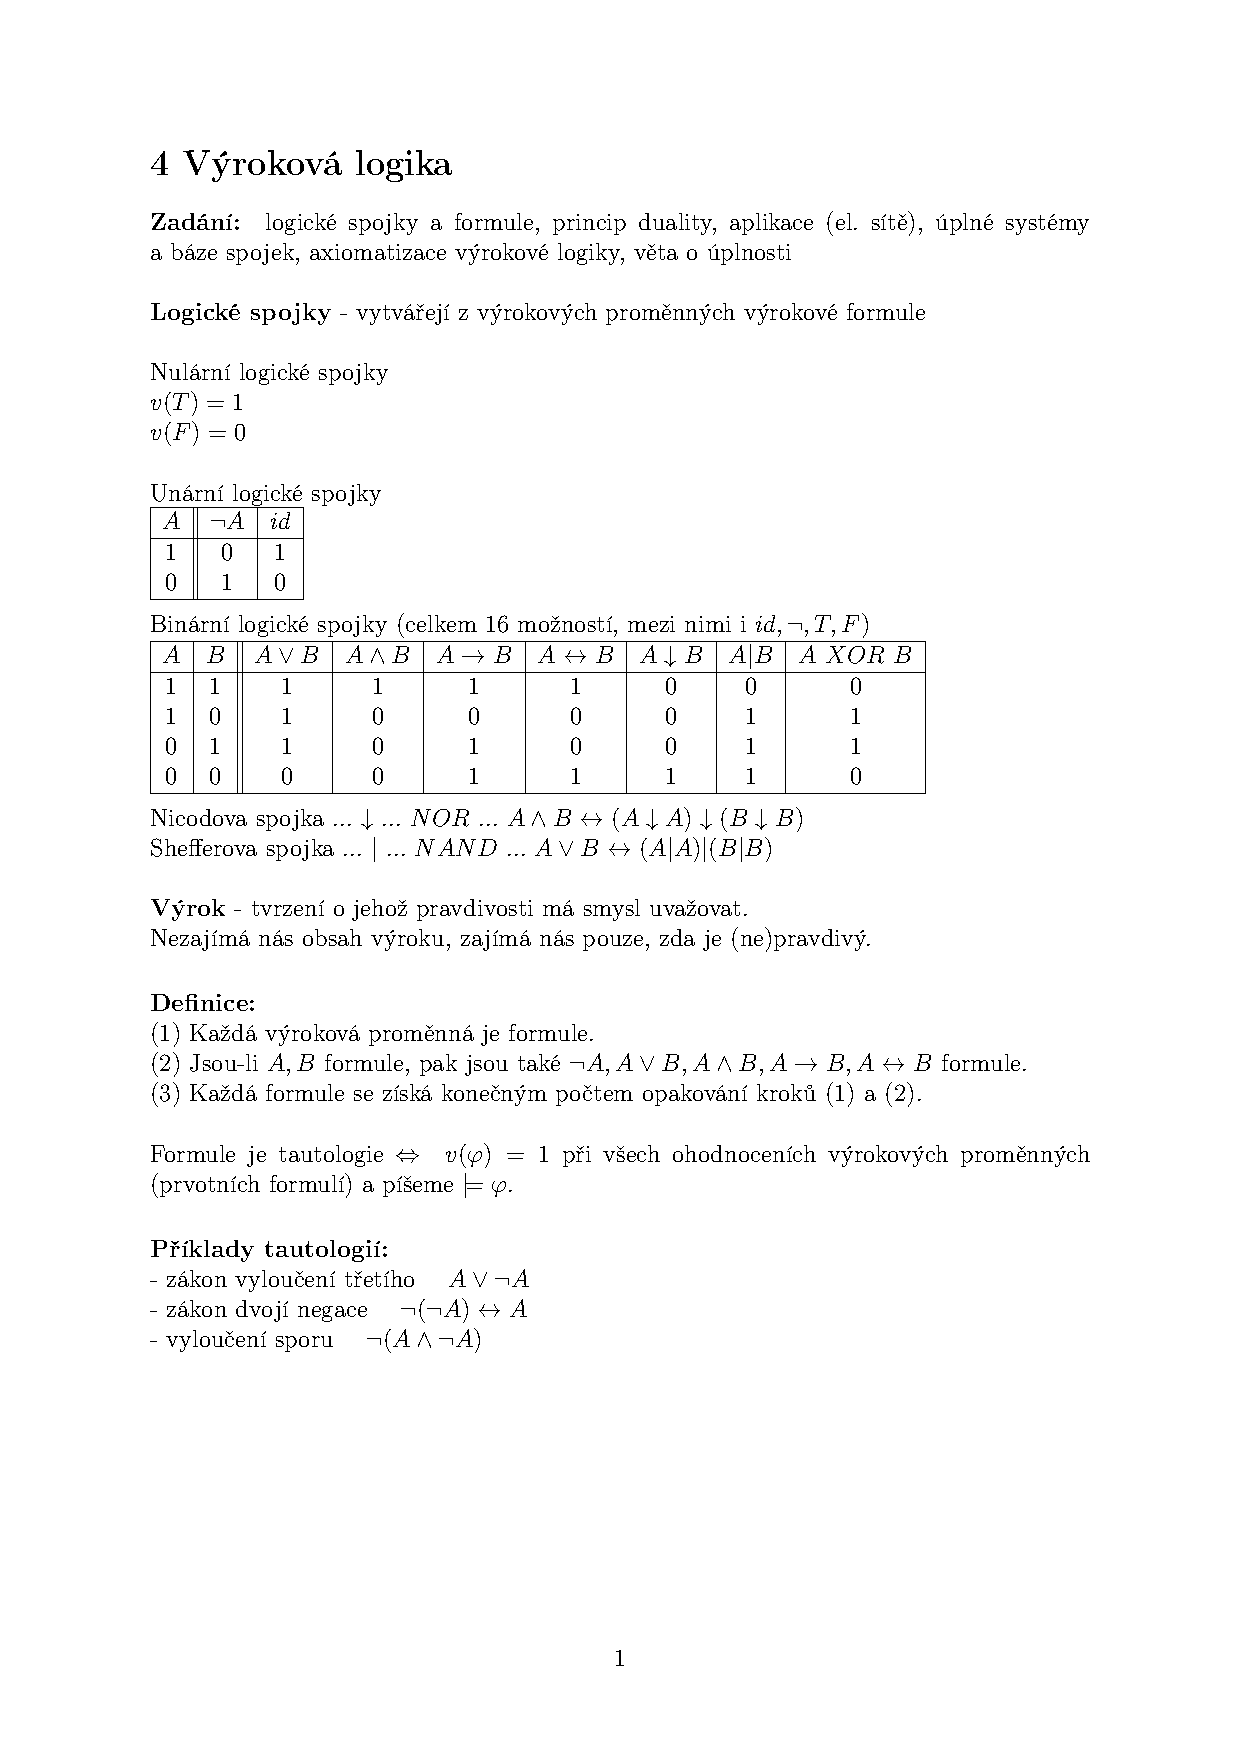
\includepdf[pages={1}]{logic_0506.pdf}
% \includepdf[pages={2}]{logic_0506.pdf}
% \includepdf[pages={3}]{logic_0506.pdf}
\paragraph*{Zadání:}
logické spojky a formule, princip duality, aplikace (el. sítě),
úplné systémy a~báze spojek, axiomatizace výrokové logiky, věta o úplnosti\\
~\\
\textbf{Logické spojky} - vytvářejí z výrokových proměnných výrokové formule\\~\\
Nulární logické spojky\\
$v(T) = 1$\\
$v(F) = 0$\\~\\
%
Unární logické spojky\\
\begin{tabular}{|c||c|c|}
\hline 
$A$ & $\neg A$ & $id$ \\ 
\hline 
1 & 0 & 1 \\ 
0 & 1 & 0 \\ 
\hline 
\end{tabular} ~\\~\\
%
Binární logické spojky (celkem 16 možností, mezi nimi i $id$ tj. identita, $\neg$, $T$ tj. tautologie, $F$ tj. negace tautologie)\\
\begin{tabular}{|c|c||c|c|c|c|c|c|c|}
\hline 
$A$ & $B$ & $A \vee B$ & $A \wedge B$ & $A \rightarrow B$ & $A \leftrightarrow B$ & $A\downarrow B$ & $A\vert B$ & $A~XOR~B$ \\ 
\hline 
1 & 1 & 1 & 1 & 1 & 1 & 0 & 0 & 0 \\ 
1 & 0 & 1 & 0 & 0 & 0 & 0 & 1 & 1 \\ 
0 & 1 & 1 & 0 & 1 & 0 & 0 & 1 & 1 \\ 
0 & 0 & 0 & 0 & 1 & 1 & 1 & 1 & 0 \\ 
\hline 
\end{tabular} ~\\~\\
Nicodova spojka ... $ \downarrow $ ... $NOR$ ... $A\wedge B \leftrightarrow (A\downarrow A)\downarrow (B\downarrow B)$\\
Shefferova spojka ... $ \vert $ ... $NAND$ ... $A\vee B \leftrightarrow (A\vert A)\vert (B\vert B)$\\~\\
%
\textbf{Výrok} - tvrzení o jehož pravdivosti má smysl uvažovat.\\
Nezajímá nás obsah výroku, zajímá nás pouze, zda je (ne)pravdivý.

\paragraph*{Definice:} ~\\
(1) Každá výroková proměnná je formule.\\
(2) Jsou-li $A, B$ formule, pak jsou také $ \neg A, A \vee B, A \wedge B, A \rightarrow B, A \leftrightarrow B $ formule.\\
(3) Každá formule se získá konečným počtem opakování kroků (1) a (2).\\
~\\
Formule je tautologie $\Leftrightarrow ~ v(\varphi ) = 1$ při všech ohodnoceních výrokových proměnných (prvotních formulí) a píšeme $\models \varphi $.
%
\paragraph*{Příklady tautologií:}~\\
- zákon vyloučení třetího ~~ $ A \vee \neg A $\\
- zákon dvojí negace ~~ $ \neg ( \neg A) \leftrightarrow A$\\
- vyloučení sporu ~~ $ \neg ( A \wedge \neg A ) $
%\newpage
\subsection*{Princip duality}
\paragraph*{Věta:}
Buď $A$ formule, v níž se vyskytují jen spojky $\neg , \vee , \wedge $.
Označme $ A ' $ formuli, která vznikne z $A$ nahrazením spojek $ \vee $, $ \wedge $
spojkami k nim duálními. Pak:\\
- $A$ tautologie $ \Leftrightarrow ~~ \neg A ' $ je tautologie\\
- je-li $(A \rightarrow B)$ tautologie, pak je také $(B' \rightarrow A')$ tautologie\\
- je-li $(A \leftrightarrow B)$ tautologie, pak je také $(A' \leftrightarrow B')$ tautologie

\paragraph*{Definice:}
Buď $A$ formule. Pak duální formulí k $A$ rozumíme $A^*$, která vznikne z $A$ záměnou spojek $ \vee , \wedge $ za spojky k nim duálními a nahrazením jednotlivých proměnných jejich negacemi.

\paragraph*{Věta:}
Buďte $A, B$ formule obsahující jen spojky $\neg , \vee , \wedge $.\\
Je-li $(A \rightarrow B)$ tautologie, pak je také $(B^* \rightarrow A^* )$ tautologie.\\
Je-li $(A \leftrightarrow B)$ tautologie, pak je také $(A^* \leftrightarrow B^* )$ tautologie.

\subsection*{Aplikace}
Spínačové obvody\\
disjunkce ... paralelní zapojení\\
konjunkce ... sériové zapojení\\
~\\
Sítě jsou ekvivalentní $\Leftrightarrow $ proud prochází oběma zároveň.\\
Minimalizace sítě\\
- minimální sít má mezi všemi sítěmi s ní ekvivalentními nejméně spínačů\\
- řešení - síť převedeme na formuli a tu upravíme na logicky ekvivalentní formuli\\
- můžeme použít Carnaughovu mapu

\paragraph*{Definice:}~\\
- \textbf{Úplným systémem spojek} výrokové logiky rozumíme takovou množinu spojek, že každou spojku výrokové logiky můžeme vyjádřit pomocí spojek z této množiny.\\
- Minimální úplný systém spojek - \textbf{báze spojek} výrokové logiky. (minimální vzhledem k množinové inkluzi)

\paragraph*{Věta:}
Jedinými bázemi spojek tvořenými jednou binární spojkou jsou $ \{ \downarrow \} $ a $ \{ \mid \} $.
%\newpage
\subsection*{Formální axiomatický systém výrokové logiky}
Abeceda\\
- množina $P$ prvotních formulí\\
- symboly pro logické spojky\\
- pomocné symboly pro závorky\\~\\
Formule\\
- všechny prvotní formule jsou formule\\
- jsou-li $A, B$ formule, pak také $\neg A, (A \rightarrow B)$ (konečná kombinace) jsou formule\\~\\
Axiomy výrokové logiky\\
(A1) $A \rightarrow (B \rightarrow A)$\\
(A2) $(A \rightarrow (B \rightarrow C)) \rightarrow (( A\rightarrow B) \rightarrow (A\rightarrow C)) $\\
(A3) $ (\neg B \rightarrow \neg A) \rightarrow (A\rightarrow B)$ ... toto je důkaz sporem\\~\\
Odvozovací pravidlo - modus ponens (pravidlo odloučení)\\
Z formulí $A, (A \rightarrow B)$ (předpoklady) se odvodí formule $B$ (závěr).

\paragraph*{Definice:}
Důkazem ve formální výrokové logice rozumíme libovolnou konečnou posloupnost $A_1 ,... A_n $ výrokových formulí takovou, že pro každé $i \leq n$ je formule $A_i$ buď axiomem nebo závěrem pravidla modus ponens.\\
$\vdash A$ ... formule $A$ je dokazatelná

\paragraph*{Věta (o dedukci):}
Nechť $T$ je množina formulí, nechť $A, B$ jsou formule.\\
Potom $T \vdash A \rightarrow B$ právě když $T \cup \{ A \} \vdash B$.

\paragraph*{Věta (o korektnosti):}
$\vdash \varphi \rightarrow \models \varphi$\\
tj. když je něco dokazatelné, tak je to tautologie

\paragraph*{Věta (o úplnosti):}
$\models \varphi \rightarrow \vdash \varphi $

\paragraph*{Lemma:} ~\\
(a) $\vdash \neg A \rightarrow (A \rightarrow B)$\\
(b) $\vdash \neg \neg A \rightarrow A$\\
(c) $\vdash A \rightarrow \neg \neg A$\\
(d) $\vdash (A\rightarrow B) \rightarrow (\neg B \rightarrow \neg A)$\\
(e) $\vdash A \rightarrow (\neg B \rightarrow \neg(A\rightarrow B)) $\\
(f) $\vdash (\neg A \rightarrow A) \rightarrow A $

\section{Predikátová logika}
% zakomentovano, protože byl vložen LaTeX kod primo... pro jistotu ponechano jako koment
% \includepdf[pages={4}]{logic_0506.pdf}
\paragraph*{Zadání:}
jazyk (termy, atomické formule a formule) a sémantika (realizace jazyka a~ohodnocení proměnných), logicky platné formule\\
~\\
Jazyk\\
- proměnné ($x$, $y$,...)\\
- speciální symboly (predikátové, funkční)\\
- výrokové spojky\\
- kvantifikátory $\forall , \exists$\\
- pomocné symboly (závorky)

\paragraph*{Term} je\\
(i) každá proměnná (i každá konstanta)\\
(ii) n-tice termů $f(t_1,t_2,...,t_n)$\\
(iii) každý term vznikne konečným počtem užití (i) a (ii)
\paragraph*{Atomická formule} ~\\
- jeden predikátový symbol $p$ aplikovaný na n-tici prvků $p(t_1,t_2,...,t_n)$
\paragraph*{Formule predikátové logiky} ~\\
(i) každá atomická formule je formule\\
(ii) jsou-li $\varphi , \psi$ formule, pak také jejich spojení pomocí spojek výrokové logiky jsou formule\\
(iii) je-li $x$ proměnná a $ \varphi $ formule, pak také $\forall x \varphi , \exists x \varphi$ jsou formule\\
(iiii) každá formule vznikne konečným počtem užití (i), (ii) a (iii)\\~\\
%
Proměnné ve formuli\\
- vázané - nachází-li se v nějaké podformuli\\
- volné - ty, které nejsou vázané\\~\\
%
Formule s čistými proměnnými\\
- otevřená formule - neobsahuje žádnou vázanou proměnnou\\
- uzavřená formule - neobsahuje žádnou volnou proměnnou

\paragraph*{Realizace $ \mathcal{R} $ jazyka} ~\\
(i) neprázdná podmnožina $M$ - univerzum\\
(ii) pro $\forall $ funkční symbol $f$ četnosti $n$ je dáno zobrazení $f_r : M^n \rightarrow M$\\
(iii)pro $\forall $ predikátový symbol $p$ četnosti $n$ ($n$-ární), kromě "$=$", je dána relace $p_r \subseteq M^n$\\~\\
%
\textbf{Ohodnocení proměnných} je libovolné zobrazení $e$ množiny všech proměnných do univerza $M$ dané realizace $\mathcal{R} $ jazyka L.\\~\\
%
Formule je \textbf{logicky platná}, jestliže pro $\forall $ realizaci $\mathcal{R} $ jazyka L je $M \models \varphi $. Píšeme $\models \varphi $.\\
Formule je pravdivá při ohodnocení $e$ v $\mathcal{R} $ ... $\mathcal{R} \models \varphi / e$\\
Formule je splněna v $\mathcal{R} $ ... $\mathcal{R} \models \varphi $

\section{Axiomatický systém predikátové logiky}
% zakomentovano, protože byl vložen LaTeX kod primo... pro jistotu ponechano jako koment
% \includepdf[pages={5}]{logic_0506.pdf}
\paragraph*{Zadání:}
axiomy a odvozovací pravidla, dokazování formulí, věta o dedukci, věty o úplnosti a bezespornosti\\~\\
%
\textbf{Axiomy výrokové logiky}\\
(A1) $A \rightarrow (B \rightarrow A)$\\
(A2) $(A \rightarrow (B \rightarrow C)) \rightarrow (( A\rightarrow B) \rightarrow (A\rightarrow C)) $\\
(A3) $ (\neg B \rightarrow \neg A) \rightarrow (A\rightarrow B)$\\~\\
%
\textbf{Axiom kvantifikátoru}\\
pokud $\varphi $ nemá volný výskyt proměnné $x$, pak $\forall x (\varphi \rightarrow \psi ) \rightarrow (\varphi \rightarrow \forall x \psi )$\\
%
\textbf{Axiom substituce}\\
pokud $t$ je term substituovatelný za $x$ do $\varphi $, pak $\forall x \varphi \rightarrow \varphi x [t]$\\
%
Je-li $L$ jazyk s rovností: \textbf{Axiom rovnosti}\\
$x_1 = y_1 \rightarrow ( ... (x_n = y_n \rightarrow (p(x_1,...,x_n)\rightarrow p(y_1,...,y_n))) ... )$\\
%
\textbf{Pravidlo odloučení} - modus ponens (MP)\\
$A, (A \rightarrow B) \vdash B$\\
%
\textbf{Pravidlo zobecnění} - modus generalis (MG)\\
$\varphi \vdash \forall x \varphi $

\paragraph*{Věta (o dedukci):}
Nechť $T$ je množina formulí, $\varphi $ je uzavřená, pak\\
$T \vdash \varphi \rightarrow \psi$ právě když $T, \varphi \vdash \psi$.\\~\\
%
Pravidlo $\forall $: Nemá-li $\varphi $ volnou proměnnou $x$: $\vdash \varphi \rightarrow \psi ~ \Rightarrow ~ \vdash \varphi \rightarrow \forall x \psi $\\
%
Pravidlo $\exists $: Nemá-li $\varphi $ volnou proměnnou $x$: $\vdash \varphi \rightarrow \psi ~ \Rightarrow ~ (\exists x \varphi ) \rightarrow \psi $

\paragraph*{Prenexní tvary formulí (dokazování formulí)} ~\\
Formule $A$ je v prenexním tvaru, jestliže má tvar $Q_1 x_1 ... Q_n x_n B$, kde\\
(i) $n \geq 0 $ a pro $\forall i=1,...,n $ je $Q_i $ buď $\forall $ nebo $\exists $\\
(ii) $x_1,...,x_n$ jsou navzájem různé proměnné\\
(iii) $B$ je otevřená formule (bez kvantifikátorů)

\paragraph*{Věta:}Ke každé formuli $A$ lze sestrojit prenexní formuli $A'$ tak, že $\vdash A \leftrightarrow A'$.% \\~\\
%Postup:\\
%bude doplněno ???

\paragraph*{Definice:} Důkaz je konečná posloupnost formulí, kde každá formule je buď axiom nebo závěr pravidla MP nebo MG.

\paragraph*{Věta o korektnosti:}
$T \vdash \varphi \Rightarrow T \models \varphi $

\paragraph*{Věta o úplnosti:}
Jestliže je $T$ teorie s jazykem $L$ a $\varphi $ je lib. formule jazyka $L$, potom $T \vdash \varphi \Leftrightarrow T \models \varphi $.\\
~\\
Teorie $T$ je bezesporná právě tehdy, když má model.



\section{Vícehodnotová logika}

\subsection{Łukasiewiczova logika}
Množinu logických hodnot budeme značit $L=\langle 0,1 \rangle$, což vyjadřuje pravdivost. Logickou proměnnou budeme nazývat takovou proměnnou, která nabývá hodnot z L. Množina logických spojek je následující:
$$S=\{\wedge, \vee,  \Rightarrow, \& \}$$
 Poslední spojka se jmenuje "odvážné a". Ve dvouhodnotové logice $\wedge$ a $\&$ splývají. Spojka \& se smí použít pouze v případě, kdy výroky, mezi které ji dáváme, jsou nezávislé co se zdroje týče (to se dá pouze předpokládat). 


\begin{definition}
\begin{itemize}
    \item Je-li $\alpha\in L \Rightarrow  \alpha $ je formule
    \item Je-li $x\textrm{ logická proměnná} \Rightarrow x$ je formule
    \item Jsou-li  $\phi$ a $\psi$ formule a $*\in S\Rightarrow (\phi * \psi )$ je logická formule
    \item Každá formule vznikla konečným použitím předešlých pravidel
\end{itemize}

\end{definition}

Dále definujeme další (pomocné) logické spojky, které umožní zjednodušit zápis.

\begin{definition}
\begin{itemize}
\item  biimplikace, oboustranná implikace: $\Leftrightarrow$ budeme psát místo $(A\Rightarrow B) \wedge (B\Rightarrow A) $
\item  Negace: $\neg$ budeme psát místo $A\Rightarrow 0$
\end{itemize}
\end{definition}

Interpretace formule nazýváme dosazení konkrétních logických hodnot do všech logických proměnných formule.

\begin{definition}
Pravdivostní ohodnocení $V(\phi)$ formule $\phi$ je zobrazení, které každé interpretaci formule $\phi$ přiřazuje logickou hodnotu z $L$.
\end{definition}


Axiomy Łukasiewiczovy logiky
\begin{itemize}
\item  $V(\alpha)=\alpha \ \ \ \forall \alpha\in L$
\item  $V(\phi \wedge \psi)=min\{ V(\phi),V(\psi)  \}$
\item  $V(\phi \vee \psi)=max\{ V(\phi),V(\psi)  \}$
\item  $V(\phi \Rightarrow \psi)=min\{1,1- V(\phi)+V(\psi)  \}$
\item  $V(\phi \& \psi)=max\{0,V(\phi)+V(\psi)-1  \}$
\end{itemize}

Klasická dvojhodnotová logika je speciálním případem výše uvedené (axiomy 2 a 5 jsou totožné).

Axiomy vícehodnotové logiky od Łukasiewicze nejsou jediné možné. Byl sestaven obecně přijímaný seznam požadavků, který by mělo splňovat pravdivostní ohodnocení. Požadavek, který je kladený na operaci, která provádí pravdivostní ohodnocení konjukce, zní, že by měla být t-normou. Požadavek kladený na disjunkci zní, že by měla být t-konormou. U implikace neexistují jednotně přijímané požadavky. Dále si uvedeme některé zobecněné implikace

\begin{itemize}
\item $I(x,y)=max\{1-x,y \}$ (Kleene-Dienes)
\item  $I(x,y)=1-x+xy$  (Rechenbach)
\item  $I(x,y)=min\{1,1-x+y\}$  (Łukasiewicz)
\item  $I(x,y)=1$ pro $x\leq y$ a $I(x,y)=y$ pro $x>y$  (Gödel)
\end{itemize}


\subsection{T-norma (trojúhelníková norma)}

\begin{definition}
Zobrazení $t:\langle 0,1\rangle \times \langle 0,1\rangle \rightarrow \langle 0,1\rangle$ se nazývá t-norma, splňuje-li následující podmínky:

\begin{itemize}
\item  t je neklesající v obou argumentech
\item  $t(x,y)=t(y,x)$  $\forall x,y\in \langle 0,1 \rangle$ (komutativita)
\item  $t(x,t(y,z))=t(t(x,y),z) $  $\forall x,y,z\in \langle 0,1 \rangle$ (asociativita)
\item $t(1,x)=x$  $\forall x\in \langle 0,1 \rangle$ (hraniční podmínka)
\end{itemize}
\end{definition}

Základní t-normy:
\begin{itemize}
\item Minimová: $T_M (x,y)=min\{x,y\}$,
\item Součinová: $T_P (x,y)=xy$,
\item Łukasiewiczova: $T_L (x,y)=max\{0,x+y-1\}$,
\item Drastický součin: $T_D(x,y)=min\{x,y\}$ pokud $max\{x,y\}=1$ jinak $T_D(x,y)=0$.
\end{itemize}



\subsection{T-konorma (trojúhelníková konorma)}

\begin{definition}
Zobrazení $s:\langle 0,1\rangle \times \langle 0,1\rangle \rightarrow \langle 0,1\rangle$ se nazývá t-konorma, splňuje-li následující podmínky:
\begin{itemize}
\item  t je neklesající v obou argumentech
\item  $s(x,y)=s(y,x)$  $\forall x,y\in \langle 0,1 \rangle$ (komutativita)
\item  $s(x,s(y,z))=s(s(x,y),z) $  $\forall x,y,z\in \langle 0,1 \rangle$ (asociativita)
\item $s(0,x)=x$  $\forall x\in \langle 0,1 \rangle$ (hraniční podmínka)
\end{itemize}
\end{definition}

Příklady t-konormy:
\begin{itemize}
\item Maximová: $S_M (x,y)=max\{x,y\}$, 
\item Pravděpodobnostní součet: $S_P(x,y)=x+y-xy$, 
\item Łukasiewiczova: $S_L (x,y)=min\{1,x+y\}$,
\item Drastický součet: $S_D(x,y)=max\{x,y\}$ pokud $min\{x,y\}=0$ jinak $S_D(x,y)=1$.
\end{itemize}







\section{NP úplné úlohy}

\section{Slovní modely}

\begin{definition}
Formule
\end{definition}

\begin{definition}
Nechť $X_1,...,X_n$ jsou slovní proměnné, $\Theta(t_1,...,t_n)$ je formule, $L_1,...,L_n$ slovní hodnoty $X_1,...,X_n$. $\mu_{L_1}(y_1),...,\mu_{L_n}(y_n)$ jsou sémantické interpretace těchto slovních hodnot. Položme $t_1=\mu_{L_1}(y_1),...,t_n=\mu_{L_n}(y_n)$, pak $\Theta(t_1,...,t_n)$ je \textbf{slovním modelem}. 
\end{definition}

\begin{definition}
$X_1,...,X_n$ jsou nezávislé slovní proměnné a $L_1,...,L_n$ jejich slovní hodnoty. Nechť $y$ je závislá slovní proměnná a $K$ její slovní hodnota.\textbf{CI-prohlášením} nazveme slovní model když $$x_1=L_1,...,x_n=L_n \quad \Longrightarrow \quad y=K$$
\end{definition}

\begin{definition}
Nechť $P_1,...,P_n$ jsou CI prohlášení, pak $P_1\wedge P_2\wedge...\wedge P_n$ nazveme \textbf{CIC} modelem a $P_1 \& P_2 \&... \& P_n$ \textbf{CI\& modelem}.
\end{definition}

\begin{definition}
Nechť $X_1,...,X_n$ jsou slovní proměnné, které definujeme, že jsou známé a slovní proměnnou $Y$, kterou definujeme, že je neznámá. $L_1,...,L_n$ nechť jsou slovní hodnoty známých proměnných. $K$ slovní hodnota neznámé proměnné. $$x_1=L_1\wedge...\wedge x_n=L_n \quad \wedge \quad Y=K$$ nazveme \textbf{CC prohlášením}
\end{definition}

\begin{definition}
Nechť $Q_1,...,Q_n$ jsou CC prohlášení. Pak $Q_1 \vee...\vee Q_n$ nazveme \textbf{CCD modelem}.
\end{definition}

Shrnutí vlastností slovních modelů:
\begin{center}
 \begin{tabular}{|| c ||c c c c||} 
 \hline
  & interpretace pravdy & citlivost na spory & citlivost na redund. info. & přezdívka \\ [0.5ex] 
 \hline\hline
 CCD & pravda je to, co tvrdí alespoň jedno prohlášení & ne & ne & naivní hazardér \\ 
 \hline
 CIC & pravda je to, co není v rozporu s libovolným prohlášením & ano & ne & zbabělý inteligent \\
 \hline
 CI\& & pravda je to, co není v rozporu s libovolným prohlášením & ano & ano & Göbbels \\ [1ex] 
 \hline
 \end{tabular}
\end{center}

\section{Matematické struktury}


\chapter{Funkce komplexní proměnné, DR, geometrie}

\section{Funkce komplexní proměnné}

\begin{definition}
Nechť $M\subseteq \overline{\mathbb{C}}=\mathbb{C}\cup \{\infty\}$ a $N\subseteq \mathbb{\overline{C}}$. Surjekci $f:M\rightarrow N$    (zobrazení na množinu = obor hodnot je celá množina N) budeme nazývat \textbf{komplexní funkcí komplexní proměnné} (dále jen funkce).
\end{definition}

\begin{definition}
$\ell\in\mathbb{\overline{C}}$ nazveme \textbf{limitou funkce $f(z)$ pro $z\rightarrow z_0$}, kde $z_0\in\mathbb{\overline{C}}$ platí-li: $$\forall O(\ell) \exists O(z_0): \forall z\in O(z_0)\backslash\{z_0\}: f(z)\in O(\ell)$$
Píšeme $$\lim_{z\to z_0}f(z)=\ell$$
\end{definition}

\begin{definition}
Řekneme, že funkce $f(z)$ je \textbf{spojitá v bodě $z_0\in\mathbb{\overline{C}}$} platí-li:
$$\lim_{z\to z_0}f(z)=f(z_0), z_0\in\mathbb{\overline{C}}$$
Tedy $$\forall O(f(z_0)) \exists O(z_0): \forall z\in O(z_0): f(z)\in O(f(z_0))$$
\end{definition}

\begin{definition}
Nechť $M\subseteq \overline{\mathbb{C}}$. Řekneme, že $f(z)$ je \textbf{spojitá v $z_0\in\overline{\mathbb{C}}$ vzhledem k množině $M$} platí-li: $$\forall O(f(z_0)) \exists O(z_0): \forall z\in O(z_0)\cap M: f(z)\in O(f(z_0))$$ 
\end{definition}

\begin{definition}
Nechť $M\subseteq \overline{\mathbb{C}}$. Řekneme, že funkce $f(z)$ je \textbf{spojiitá na množině $M$}, pokud je spojitá v každém bodě množiny $M$ vzhledem k množině $M$.
\end{definition}

\begin{definition}
Řekneme, že funkce $f(z)$ je \textbf{ohraničená na množině $M\subseteq \overline{\mathbb{C}}$}, když
$$\exists O(0): f(z)\in O(0) \forall z\in M$$
\end{definition}

\begin{theorem}[1. Weierstrass]
Nechť funkce $f(z)$ je spojitá na kompaktní množině $M$, pak je na této množině ohraničená.
\end{theorem}

\textit{Kompaktní množina = množina ohraničená a uzavřená}

\begin{theorem}[2. Weierstrass]
Nechť funkce $f(z)$ je spojitá a ohraničená na kompaktní množině $M$, pak funkce $|f(z)|$ nabývá na této množině svého maxima a minima.
\end{theorem}

\subsection{ELEMENTÁRNÍ FUNKCE}

\subsubsection{Polynomy}
$$f(z)=a_nz^n+a_{n-1}z^{n-1}+..+a_2z^2+a_1z+a_0$$
$$a_0,a_1,..,a_n\in\mathbb{C}; a_n\neq0$$
$n$ - stupeň polynomu
$f(\alpha)=0 \Rightarrow \alpha$ - kořen polynomu

rozklad na kořenové činitele: $f(z)=a_n(z-z_1)^{l_1}(z-z_2)^{l_2}..(z-z_k)^{l_k}$, $l_1,l_2,..,l_k$ - násobnosti kořenů $z_1,z_2,..,z_k$; $l_1+l_2+..+l_k=n$

\subsubsection{Racionální funkce}
$$f(z)=\frac{P_n(x)}{Q_m(z)}$$
$P_n(z)$ - polynom stupně $n$

$Q_m(z)$ - polynom stupně m

$n<m$ - ryzí funkce

$n\geq m$ - neryzí funkce

\begin{theorem}
Nechť $f(z)=\frac{P_n(x)}{Q_m(z)}$ je neryzí racionální funkce. Pak tuto funkci lze zapsat ve tvaru: $$\frac{P_n(x)}{Q_m(z)}=R_{n-m}(z)+\frac{S_k(z)}{Q_m(z)}; k<m$$
$R_{n-m}$ - polynom stupně $n-m$
$\frac{S_k(z)}{Q_m(z)}$ - ryzí racionální funkce
\end{theorem}

%
% ^.

\begin{theorem}[O rozkladu na parciální zlomky]
Nechť $\frac{P_n(x)}{Q_m(z)}$ je ryzí racionální funkce. Nechť $Q_m(z)=a_m(z-z_1)^{l_1}(z-z_2)^{l_2}..(z-z_k)^{l_k}$ je rozklad polynomu $Q_m(z)$ na kořenové činitele. Pak lze funkci $\frac{P_n(x)}{Q_m(z)}$ zapsat v součtu m parciálních zlomků, přičemž každému z kořenů $z_1,z_2,..,z_k$ přísluší postupně $l_1,l_2,..,l_k$ parciálních zlomků tvaru: $\frac{b_1}{z-z_s},\frac{b_2}{(z-z_s)^2},..,\frac{b_{l_s}}{(z-z_s)^{l_s}}; s=1,2,..,k$
\end{theorem}

\subsubsection{Exponenciální funkce}
Ozn. $e^z$, $\exp(z)$, $\exp z$
\begin{definition}
Nechť $z=x+iy$. Pak $e^z=e^x(\cos y +i\sin y)$.
\end{definition}

\textit{Vlastnosti funkce $e^z$:} 
\begin{enumerate}
\item $Im z= 0 \Rightarrow e^x$
\item $e^z$ - periodická funkce s periodou $2\pi i$
\item $e^z=0$ - neřešitelná v $\mathbb{C}$
\item $e^{z_1}\cdot e^{z_2}=e^{z_1+z_2}$
\item $\lim_{z \to \infty}e^z$ - neexistuje (protože platí 2.)
\item $|\mathrm{e}^{z}|=\mathrm{e}^x$ 
\end{enumerate}

Pozor $e^z$ není $e^z$, na komplexní číslo nelze umocňovat!

\subsubsection{Goniometrické funkce}

$$\sin z = \frac{1}{2i}(e^{iz}-e^{-iz})$$
$$\cos z = \frac{1}{2}(e^{iz}+e^{-iz})$$
$$\tan z = \frac{\sin z}{\cos z}$$
$$cotg z = \frac{\cos z}{\sin z}$$

\textit{Vlastnosti funkcí $\sin z$ a $\cos z$:} 
\begin{enumerate}
\item periodické funkce s periodou $2\pi$
\item neexistují limity těchto funkcí pro $z\rightarrow +\infty$
\item oborem hodnot těchto funkcí je celé $\mathbb{C}$
\end{enumerate}

\textit{Vzorce pro práce s goniometrickými funkcemi platné v reálném oboru zůstávají platné i pro práci v komplexním oboru.}

\section{Derivace funkce v komplexním oboru} 

\begin{definition}
Derivací funkce $f(z)$ v bodě $z_0\in\mathbb{C}$, značíme $f'(z_0)$ , nazveme $$\lim_{z\to z_0}\frac{f(z)-f(z_0)}{z-z_0},$$pokud je tato limita konečná. Pokud tato limita neexistuje nebo je rovna $\infty$, řekneme, že neexistuje derivace funkce $f(z) $ v bodě $z_0$
\end{definition}

\textit{Veškeré vzorce pro výpočet derivací včetně derivací elementárních funkcí, které platí v reálném oboru, platí i v komplexním oboru.}

\begin{definition}
Řekneme, že funkce $f(z)$ je \textbf{holomorfní v bodě} $z_0\in\mathbb{C}$, pokud existuje takové okolí $O(z_0)$ bodu $z_0$, že existuje derivace funkce $f(z)$  $\forall z \in O(z_0)$.
\end{definition}

\begin{definition}
Řekneme,  že funkce $f(z)$ je \textbf{holomorfní na otevřené množině} $M\subseteq\mathbb{\overline{C}}$, když je holomorfní v každém bodě množiny $M$.
\end{definition}

\textit{Holomorfnost nelze definovat na množině, která není otevřená. \\ Problém lze obejít, když se definuje derivace vzhledem k množině.}

\subsection{Geometrická interpretace derivace}
Význam derivace:
\begin{enumerate}
\item $|f'(z_0)|$ - koeficient homometrie (zvětšení, zmenšení okolí) ($k \doteq |f'(z_0)|$ - viz. obrázek s kontrolním chroustem)
\item $arg f'(z_0)$ - úhel otočení ($\varphi \doteq arg f'(z_0)$ - viz. obrázek s kontrolním chroustem - v případě infinitezimálního chrousta "=")
\end{enumerate}
\begin{theorem}
    Nechť funkce $f(z)$ je holomorfní v bodě $z_0\in\mathbb{C}$. 
    
    Nechť $O(z_0)$ je okolí, na kterém je funkce $f(z)$ holomorfní. 
    
    Nechť $\varphi(t)$, $t\in\langle a,b\rangle$ je křivka taková, že $[\varphi]\subseteq O(z_0)$, $z_0\in\varphi$ je bod, kterým křivka $\varphi$ prochází a $z_0\neq\varphi(a)$, $z_0\neq\varphi(b)$.
    
    Nechť $p$ je orientovaná tečna ke grafu $[\varphi]$ v bodě $z_0$ a $q$ je orientovaná tečna ke grafu $[f(\varphi)]$ v bodě $f(z_0)$.
    
    Pak platí, že $\sphericalangle (p,q) = \arg f'(z_0)$.
\end{theorem}

\begin{theorem}
Zachovejme označení z předešlé věty. Navíc označme $z_0=\varphi(t_0)$, dále $\Delta_h\varphi=|\varphi(t_0+h)-\varphi(t_0)|$, $\psi = f(\varphi)$, $\Delta_h\psi=|\psi(t_0+h)-\psi(t_0)|$.

Potom platí $$\lim_{h\to 0}\frac{\Delta_h\psi}{\Delta_h\varphi}=|f'(z_0)|$$
\end{theorem}

\subsection{Funkce holomorfní v $\infty$}
\begin{definition}
Řekneme, že funkce $f(z)$ je holomorfní v bodě $\infty$, pokud je v bodě $\infty$ spojitá a funkce $f(\frac{1}{z})$ je holomorfní v bodě $0$.
\end{definition}

\begin{definition}
Nechť funkce $f(z)$ je holomorfní v bodě $\infty$, pak definujeme, že $f'(\infty)=\frac{1}{f'(\frac{1}{z})}|_{z=0}$
\end{definition}

\subsection{Cauchy-Riemannovy podmínky}
\begin{definition}
Každou funkci $f(z)$ lze zapsat ve tvaru: $$f(z)=u(x,y)+i v(x,y)$$ kde $z=x+iy$. 

$u(x,y)$ - $Re f$ - reálná část funkce $f$
$v(x,y)$ - $Im f$ - imaginární část funkce $f$
\end{definition}

\begin{theorem}
Mějme funkci $f(z)=u(x,y)+i v(x,y)$. Nechť $z_0=x_0+i y_0$, nechť $O(z_0)$ je okolí bodu $z_0$ a $O([x_0,y_0])$ je totéž okolí chápáno v $\mathbb{R^2}$.

Potom platí, že funkce $f(z)$ je holomorfní v bodě $z_0$ právě, když obě funkce $u$ a $v$ jsou diferencovatelné na $O([x_0,y_0])$ a platí pro ně současně následující podmínky:
\begin{enumerate}
\item $\frac{\partial u(x_0,y_0)}{\partial x}=\frac{\partial v(x_0,y_0)}{\partial y}$
\item $\frac{\partial u(x_0,y_0)}{\partial y}=-\frac{\partial v(x_0,y_0)}{\partial x}$
\end{enumerate}
\end{theorem}

\subsection{Křivky a oblasti}
\begin{definition}
Křivka $\varphi(t), t\in\langle a,b\rangle$ se nazývá \textbf{jordanova}, pokud splňuje:
\begin{enumerate}
\item $\varphi$ je uzavřená (tj. má totožný počáteční i koncový bod)
\item $\varphi$ je prostá (tj. platí: 
\begin{enumerate}
\item $t_1\neq t_2 \Rightarrow\varphi(t_1)\neq\varphi(t_2)$, $\forall t_1,t_2\in(a,b)$
\item $\varphi$ nelze rozložit na dvě nebo více křivek splňujících podmínku (a))
\end{enumerate}
\item $\infty\notin[\varphi]$ = neprochází nekonečnem
\end{enumerate}
\end{definition}

\subsection{Taylorovy řady}
\begin{theorem}[Taylorova]
Nechť funkce $f(z)$ je holomorfní v bodě $z_0\in\mathbb{C}$. Pak  existuje takové okolí $O(z_0)$ bodu $z_0$, že platí $$f(z)=\sum_{n=0}^\infty a_n(z-z_0)^n,$$ pro každé  $ z\in O(z_0)$, přičemž  $a_n=\frac{f^{(n)}(z_0)}{n!}=\frac{1}{2\pi i}\int_{\varphi}\frac{f(z)}{(z-z_0)^{n+1}}dz$(z Cauchy. int. vzorce)

$\varphi$ - lib. hladká jordanova křivka s vlastností: $z_0\in int\varphi$, $[\varphi\in O(z_0)]$.

Tj. Taylorova řada.
\end{theorem}

\begin{theorem}
Nechť $$f(z)=\sum_{n=0}^{\infty}a_n(z-z_0)^n$$ je Taylorova řada funkce $f(z)$ v bodě $z_0\in\mathbb{C}$. 

Poloměr konvergence je: 
\begin{itemize}
\item $r=\infty$, v případě, že $f(z)$ je holomorfní v $\mathbb{C}$
\item $r=\inf_{w\in P}\rho(z_0,w)$, kde $P$ je množina všech bodů, ve kterých $f(z)$ není holomorfní.
\end{itemize}
\end{theorem}


\textit{\begin{enumerate} 
\item Je-li funkce $f(z)$ holomorfní v celém $\mathbb{C}$, pak tuto funkci lze ztotožnnit s její Taylorovou řadou (mocninnou řadou).
\item Pokud $f(z)$ je holomorfní v celé Gaussově rovině s vyjímkou některých bodů či oblastí. Pak ji s mocninnou řadou ztotožnit  nemůžeme. Můžeme ji s ní ztotožnit pouze na okolí lib. bodu, ve kterém je taot funkce holomorfní. Je zřejmé, že k pokrytí celého $\mathbb{C}$ potřebujeme nekonečně mnoho Taylorových řad. (viz. Laurentovy řady). 
\end{enumerate}}

\begin{theorem}{O rozvoji holomorfní funkce v mocninou řadu}
Funkce $f(z)$ je holomorfní v bodě $z_0  \in \mathbb{C}$, právě když existuje takové okolí $O(z_0)$ bodu $z_0$, že funkci $f(z) $ lze vyjádřit na tomto okolí ve tvaru součtu Taylorovy řady a koeficienty jsou jednoznačně určeny předpisem pro $a_n$ .

\end{theorem}
\subsection{Laurentovy řady}
\begin{definition}
$$\sum_{n=-\infty}^{\infty}a_n(z-z_0)^n$$ nazýváme \textbf{Laurentova řada se středem $z_0\in\mathbb{C}$}

$...,a_{-2},a_{-1},a_0,a_1,a_2,...\in\mathbb{C}$ - \textbf{koeficienty Laurentovy řady}

Laurentovu řadu musíme rozdělit na 2 nekonečné řady:
\begin{align*}
\underbrace{\sum_{n=1}^{\infty}\frac{a_{-n}}{(z-z_0)^n}}_{\text{hlavní část Laurentovy řady}}+\underbrace{\sum_{n=0}^{\infty}a_n(z-z_0)^n}_{\text{regulární část Laurentovy řady}}
\end{align*}
Konverguje-li  v bodě $z \in \mathbb{C}$ (respektive  konverguje bodově/absolutně/stejnoměrně/skoro stejnoměrně na množině $M\subset \mathbb{C}$ ) současně hlavní i regulární část Laurentovy řady, řekneme, že konverguje samotná Laurentova řada v bodě $z \in \mathbb{C}$  (respektive  konverguje bodově/absolutně/stejnoměrně/skoro stejnoměrně na množině $M\subset \mathbb{C}$ ) a definujeme $$\sum_{n=-\infty}^{\infty}a_n(z-z_0)^n=S=S_H+S_R$$

$S_H$ - součet hlavní řady

$S_R$ - součet regulární řady
\end{definition}

\begin{definition}
Laurentova řada se středem v bodě $\infty$ má tvar:
\begin{align*}
\sum_{n=-\infty}^{\infty}a_nz^n=\underbrace{\sum_{n=0}^{\infty}\frac{a_{-n}}{z^n}}_{\text{regulární část Laurentovy řady}}+\underbrace{\sum_{n=1}^{\infty}a_nz^n}_{\text{hlavní část Laurentovy řady}}
\end{align*}
\end{definition}

\textit{\textbf{Pozor!} Člen $a_0$ patří vždy do regulární části.}

\begin{theorem}
Nechť Laurentova řada má netriviální obor konvergence. Pak funkce 
$$
f(z)=\sum_{n=-\infty}^{\infty} a_n (z-z_0)^n
$$
definovaná jako součet Laurentovy řady je holomorfní na mezikruží konvergence $M(u_0,r,R)$ této řady.
\end{theorem}
\begin{theorem}[Laurentova]
Nechť funkce $f(z)$ je holomorfní na mezikruží $M(z_0,r,R)$, pak existuje Laurentova řada v bodě $z_0$, která konverguje k funkci $f(z) $ na množině $M(z_0,r,R)$ absolutně a skoro stejnoměrně. Tedy tuto funkci lze zapsat ve tvaru Laurentovy řady $$f(z)=\sum_{n=-\infty}^{\infty}a_n(z-z_0)^n,$$přičemž platí $a_n=\frac{1}{2\pi i}\int_{\varphi}\frac{f(z)}{(z-z_0)^{n+1}}dz$, kde $\varphi$ je libovolná po částech hladká kladně orientovaná Jordanova křivka taková, že $[\varphi]\subseteq M(z_0,r,R)$ a $z_0\in int\varphi$.

Koeficienty této Laurentovy řady jsou určeny jednoznačně.
\end{theorem}

Poznámka: Na rozdíl od Taylorovy řady, může mít funkce $f(z)$ více různých Laurentových řad se středem v bodě $z_0$. Každá z těchto řad ovšem bude mít jiné mezikruží konvergence. Na každém mezikruží už je pak Laurentova řada určena jednoznačně.

\subsection{Singulární body}
\begin{definition}
Řekneme, že bod $z_0\in \overline{\mathbb{C}}$ je \textbf{singulárním bodem} (izolovaným singulárním bodem) funkce $f(z)$, pokud platí:
$\exists O(z_0)$ takové, že $f(z)$ je holomorfní na $O(z_0)\diagdown \{z_0\}$ a v bodě $z_0$ holomorfní není. 

Bod $z_0=\infty$ budeme vždy nazývat singulárním bodem (i když funkce $f(z)$ je holomorfní v $\infty$).
\end{definition}

\begin{definition}
Nechť $z_0\in \overline{\mathbb{C}}$ je izolovaný  singulární bod $f(z)$, nechť $\sum_{n=-\infty}^{+\infty}a_n(z-z_0)^n$ je Laurentova řada funkce $f(z)$ v bodě $z_0$ na mezikruží $M(z_0,0,R), R>0$. Řekneme, že bod $z_0$ je: 
\begin{enumerate}
\item \textbf{odstranitelný} singulární bod funkce $f(z)$, pokud hlavní část uvedené Laurentovy řady má všechny koeficienty $=0$.
\item \textbf{pól}, má-li hlavní část uvedené Laurentovy řady nenulový konečný počet nenulových koeficientů.
\item \textbf{podstatně} singulární bod, má-li hlavní část uvedené Laurentovy řady nekonečný počet nenulových koeficientů.
\end{enumerate}
\end{definition}

\begin{definition}
Řekneme, že funkce $f(z)$ má v bodě $z_0=\infty$ podstatně singulární bod, pokud hlavní část Laurentovy řady má nekonečný počet nenulových koeficientů, v opačném případě řekneme, že v bodě $z_0=\infty$ je pól.
\end{definition}

\begin{theorem}
Nechť $z_0\in \overline{\mathbb{C}}$ je izolovaný singulární bod funkce $f(z)$. pak platí
\begin{enumerate}
\item nechť $z_0\in\mathbb{C}$, pak platí, že $z_0$ je podstatně singulární bod právě tehdy, když $\lim_{z\rightarrow z_0}f(z)$ neexistuje.
\item nechť $z_0\in\mathbb{C}$, pak platí, že funkce $f(z)$ má v bodě $z_0$ pól právě, když $\lim_{z\rightarrow z_0}f(z)=\infty$
\item nechť $z_0\in\mathbb{C}$, pak platí, že funkce $f(z)$ má v bodě $z_0$ odstranitelný singulární bod právě tehdy, když $\lim_{z\rightarrow z_0}f(z)\in\mathbb{C}$ (=je konečná).
\end{enumerate}
\end{theorem}

\subsubsection{Odstranitelné singulární body}
Nechť v bodě $z_0\in\mathbb{C}$ je odstranitelný singulární bod. Pak na $M(z_0,0,R)$ má Laurentova řada funkce $f(z)$ tvar $\sum_{n=0}^{\infty}a_n(z-z_0)^n$, tj. je to mocninná řada, jejíž součet je holomorfní v bodě $z_0$. 

To je možné jedině v těchto 2 případech:
\begin{itemize}
\item funkce $f(z)$ není definovaná v $z_0$ nebo
\item funkce $f(z)$ byla původně v $z_0$ holomorfní a nějaký "sabotér" změnil v bodě $z_0$ hodnotu.
\end{itemize}

\begin{theorem}
Nechť funkce $f(z)$ má v bodě $z_0\in\mathbb{C}$ odstranitelný singulární bod, pak funkce
\begin{align*}
g(z) = 
\begin{cases}
	f(z) & z \neq z_0 \\
    \lim_{z\rightarrow z_0}f(z) & z=z_0
\end{cases}
\end{align*}
je holomorfní v bodě $z_0$.
\end{theorem}

\begin{definition}
Funkci $g(z)$ z předešlé věty budeme nazývat funkcí $f(z)$ s odstranitelným singulárním bodem.
\end{definition}

Z předešlého plyne, že odstranitelné singulární body můžeme dále ignorovat, protože je lze vždy odstranit.

\subsubsection{Póly}
\begin{definition}
Nechť funkce $f(z)$ má v bodě $z_0\in\mathbb{C}$ pól. Nechť $k\in\mathbb{N}$ má vlastnost: $a_{-k}\neq 0$, kde $$\sum_{n=-k}^{\infty}a_n(z-z_0)^n$$ je Laurentova řada funkce $f(z)$ na mezikruží $M(z_0,0,R), R>0$. Nechť platí $a_{-n}=0 \forall n > k$, pak řekneme, že $z_0$ je pól řádu $k$.
\end{definition}

\begin{definition}
Nechť $z_0=\infty$ je pól funkce $f(z)$. Platí-li $$\lim_{z\rightarrow\infty}\frac{f(z)}{z^k}\in\mathbb{C}\diagdown\{0\},$$ pak řekneme, že $z_0$ je pól řádu $k$.
\end{definition}

$k$ v předešlé definici je definováno jednoznačně, protože platí: $$\lim_{z\rightarrow \infty}\frac{f(z)}{z^k}=\infty$$ v případě, že $k$ je příliš malé. $$\lim_{z\rightarrow \infty}\frac{f(z)}{z^k}=0$$ v případě, že $k$ je příliš velké. Existuje pouze jedno $k$, pro které nenastane ani jeden z těchto 2 případů.

\begin{theorem}
Nechť funkce $f(z)$ má v bodě $z_0\in\mathbb{C}$ pól řádu $k$, pak funkce $\frac{1}{f(z)}$ má v bodě $z_0$ $k-$násobný kořen.
\end{theorem}

$k-$násobný kořen $\alpha$: $f(\alpha)=0,f'(\alpha)=0,f^{(k-1)}(\alpha)=0,f^{(k)}(\alpha)\neq 0$

\begin{theorem}
Nechť funkce $f(z)$ má v bodě $z_0\in\mathbb{C}$ pól řádu $k$. Nechť $$\sum_{n=-k}^{\infty}a_n(z-z_0)^n$$ je Laurentova řada funkce $f(z)$ na $M(z_0,0,R)$. Pak funkce $(z-z_0)^kf(z)$ má v bodě $z_0$ odstranitelný singulární bod a po odstranění tohoto bodu je holomorfní na $K(z_0,R)$.
\end{theorem}

\subsubsection{Podstatně singulární body}
\begin{theorem}[Picard]
Nechť funkce $f(z)$ má v bodě $z_0\in\overline{\mathbb{C}}$ podstatně singulární bod. Nechť $O(z_0)$je libovolné okolí bodu $z_0$. Pak na $O(z_0)$ funkce $f(z)$ nabývá všech komplexních hodnot s případnou výjimkou jediné.
\end{theorem}

\begin{figure}[H]
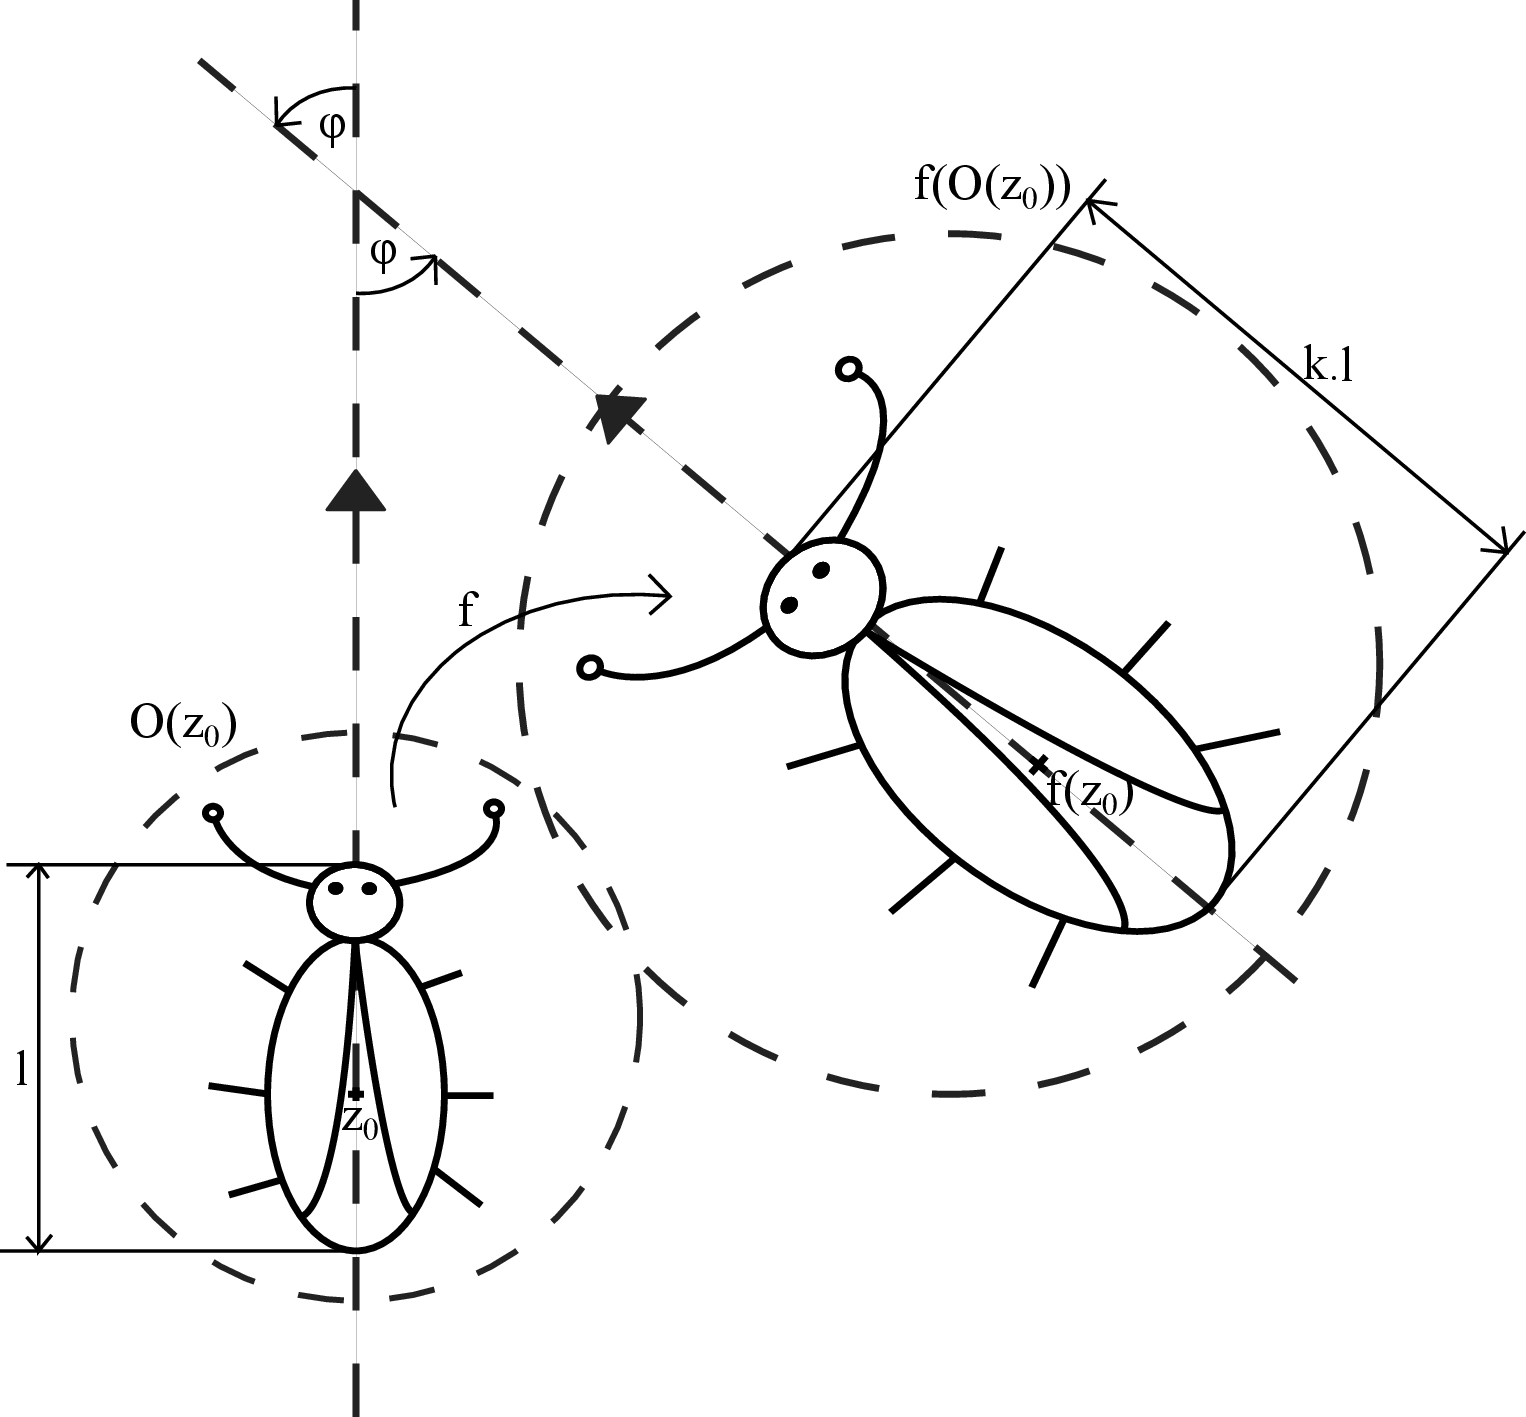
\includegraphics[scale=0.25]{Obrazky/Chroust.png}
\caption{Infinitezimální chroust}
\end{figure}


\section{Integrál v komplexním oboru}
\begin{definition}
	Mějme funkci $f(z)$, která má definiční obor $M \subseteq \mathbb{C}$. Nechť $\varphi(t), t \in \langle a,b \rangle$ je po částech hladká křivka taková, že její graf je podmnožina $M$ ($[\varphi] \subseteq M$). Pokud existuje $\int_a^b f(\varphi(t))\varphi'(t)\, \mathrm{d} t$, řekneme, že $f(z)$ je integrovatelná po křivce $\varphi$ a tento integrál značíme$\int_{\varphi} f(z)\, \mathrm{d} z$.
\end{definition}

\begin{definition}
	Nechť $\varphi(t), t \in \langle a,b \rangle$ je po částech hladká křivka. Délkou křivky nazýváme hodnotu integrálu $\int_a^b |\varphi'(t)|\, \mathrm{d} t$
 \end{definition}

\begin{definition}
(\textbf{Primitivní funkce)} Mějme funkci $f(z)$, která je definovaná na jednoduše souvislé oblasti $D \subseteq \mathbb{C}$. Řekneme, že funkce $F(z)$ je primitivní funkcí k $f(z)$, pokud $F'(z)=f(z), \forall z \in D$. Primitivních funkcí je nekonečně mnoho.
\end{definition}

\begin{theorem}
	Nechť \fce  $f(z)$ je holomorfní na $D$. Pak $\int_{\varphi}f(z) \, \dd z $ nezávisí na integrační cestě v $D$. Zapisujeme jej $\int_{z_1}^{z_2}f(z) \, \dd z = F(z_2)-F(z_1)$.
\end{theorem}

\begin{theorem}
	Následující 3 tvrzení jsou ekvivalentní na libovolné jednoduše souvislé oblasti $D \subseteq \mathbb{C}$
	\begin{itemize}
		\item Funkce $f(z)$ je holomorfní na $D$
		\item K funkci $f(z)$ existuje $F(z)$ na $D$
		\item $\int_{\varphi} f(z)\,  \dd z$ nezávisí na integrační cestě v $D$ 
	\end{itemize}
\end{theorem}

\begin{theorem}
\textbf{(Cauchyova věta- 1.verze)} Nechť $D \subseteq \mathbb{C} $ je jednoduše souvislá oblast a nechť $f(z)$ je funkce holomorfní na oblasti $D$ $\varphi$. Potom pro každou po částech hladkou Jordanova křivu takovou, že graf $[\varphi]\subset D $,  platí $\int_{\varphi} f(z)\, \dd z = 0.$
\end{theorem}



\begin{theorem}
\textbf{(Cauchyova věta- 2.verze)} Nechť $\varphi$ je po částech hladká Jordanova křivka a \fce $f(z)$ nechť je holomorfní na int$\varphi$ a je spojitá a ohraničená na $\overline{int\varphi}$. Pak platí, že $\int_{\varphi} f(z)\, \dd z=0.$  
\end{theorem}




%%%%%%%%%%%%%%%%%%%%%%%%%%%%%%%%%%%%%%%%%%%%%%%%%%%%%%%%%%%%%%
\textbf{Cauchyův integrální vzorec:}
Nechť $\varphi$ je po částech hladká kladně orientovaná Jordanova křivka. Nechť \fce\footnote{K výpočtu stačí znát funkcí jen na křivce $\varphi$} \fz je holomorfní na int$\varphi$, spojitá a ohraničená na $\overline{int\varphi}$. Potom platí $$f(z)=\frac{1}{2\pi 
i }\int_{\varphi}\frac{f(w)}{w-z}\, \dd w, \forall z \in \text{int}\varphi$$


\textbf{Cauchyův integrální vzorec pro n-tou derivaci:}
Nechť platí předpoklady předchozí věty. Potom platí:
$$f^{(n)}(z)=\frac{n!}{2\pi i}\int_{\varphi}\frac{f(w)}{(w-z)^{n+1}}\, \dd w, \forall z \in \text{int}\varphi$$

\begin{theorem}
	\textbf{(O jednoznačnosti holomorfní \fce)}
	Mějme \fce $f(z),g(z)$, které jsou holomorfní na oblasti $D \subset \CC$. Označme $M$ množinu všech bodů $z$, pro které platí $f(z)=g(z)$ tzn. $M=\{ z \in D | f(z)=g(z)\}$. Existuje-li v množině $M$ hromadný bod, pak pro každé $z\in D$ platí $f(z)=g(z)$.
	
\begin{dusledek}
	Zadám holomorfní funkci na reálné ose, libovolném kousku Gauss. roviny s nenulovou plochou, grafu libovolné křivky $\Rightarrow$ \fce je zadána v celém $\CC$.
\end{dusledek}
\end{theorem}

\begin{definition}
	\textbf{Rezidua}
	Nechť \fce \fz je holomorfní v nějakém okolí $O(z_0)$ bodu $z_0 \in \overline{\CC}$  s případnou výjimkou bodu $z_0$.
    \begin{itemize}
    \item Nechť $z_0 \in \CC$. Nechť   $\sum_{n=-\infty}^{\infty}a_n(z-z_0)^n$ je Laurentova řada funkce \fz, která konverguje k funkci \fz na množině $O(z_0)\setminus \{z_0\}$. Reziduem funkce \fz v bodě $z_0$ nazveme koeficient $a_{-1}$ Laurentovy řady a zavedem označení $\mathrm{Res}_{z=0} f(z)=a_{-1}$  
\item  Nechť $z_0=\infty$. Nechť  $\sum_{-\infty}^{\infty} a_nz^n$ je Laurentova řada funkce \fz se středem v bodě $\infty $, která kon verguje k funkci \fz na množině $O(\infty)\setminus \{\infty\}$. Reziduem funkce \fz v bodě $\infty $ nazveme koeficient $-a_{-1}$ Laurentovy řady a zavedeme označení $Res_{z=\infty} \, f(z)=-a_{-1}$.
    \end{itemize}
\end{definition}

\begin{theorem}
Nechť $z_0\in \CC$ a nechť funkce \fz je holomorfní na nějakém okolí $O(z_0)$ bodu $z_0$ s případnou výjimkou bodu $z_0$. Pak platí 
\begin{equation*}
\mathrm{Res}_{z=z_0}f(z)=\frac{1}{2\pi i}\int_{\varphi_{\rho}}f(z) \, \mathrm{d} z,
\end{equation*}
 kde $\varphi_{rho}(t)=z_0+\rho\mathrm{e}^{it}, t \in \langle 0,2\pi \rangle$ a $\rho$ je voleno tak, aby $[\varphi_{\rho}] \subset O(z_0) \setminus \{z_0\}$.
 
 A nechť  $z_0=\infty $ a nechť funkce \fz je holomorfní na nějakém okolí $O(\infty)$ bodu $\infty$ s případnou výjimkou bodu $\infty$. Pak platí 
\begin{equation*}
\mathrm{Res}_{z=\infty}f(z)=-\frac{1}{2\pi i}\int_{\varphi_{\rho}}f(z) \, \mathrm{d} z,
\end{equation*}
 kde $\varphi_{rho}(t)=\rho\mathrm{e}^{it}, t \in \langle 0,2\pi \rangle$ a $\rho$ je voleno tak, aby $[\varphi_{\rho}] \subset O(\infty) \setminus \{\infty\}$.
 \end{theorem}

\begin{theorem}
	Nechť \fce \fz má v bodě $z_0 \in \CC$ pól řádu $k$, tak platí, že 
	$$Res_{z=z_0} \, f(z)=\frac{1 }{(k-1)!} \lim_{z\rightarrow z_0}[(z-z_0)^k \, f(z)]^{(k-1)}$$
\end{theorem}
\begin{theorem}
	Nechť \fce \fz má v bodě $\infty$ pól řádu $k$, kde $k \geq -1$, potom platí, že 
	$$Res_{z=\infty} f(z) = \frac{(-1)^k}{(k+1)!} \lim_{z \rightarrow \infty} z ^{k+2}f(z)^{(k+1)}$$
	Pokud $k<-1$, pak $Res_{z=\infty}(f)=0$
\end{theorem}
%%%%%%%%%%%%%%%%%%%%%%%%%%%%%%%%%%%%%%%%%%%%%%%%%%%%%%%%%%%%%%


%%%%%%%%%%%%%%%%%%%%%%%%%%%%%%%%%%%%%%%%%%%%%%%%%%%%%%%%%%%%%%
\begin{theorem}
	Nechť \fce \fz je holomorfní v celém $\CC$ s výjimkou konečného počtu singulárních bodů $z_1,z_2,\ldots, z_n. $ Označme $z_{n+1}=\infty$, pak platí  $\sum_{k=1}^{n+1}\text{Res}_{z=z_k}\, f(z)=0$.  
\end{theorem}

\begin{theorem}
\textbf{(Reziduální věta I)}
Nechť \fce \fz je holomorfní na jednoduše souvislé oblasti $D \subseteq \CC $ s výjimkou konečného počtu singulárních bodů $z_1,z_2,\ldots, z_k \in D.$ Nechť $\varphi$ je po částech hladká kladně orientovaná Jordanova křivka taková, že $[\varphi] \subseteq D $ a její graf neprochází žádným singulárním bodem. Označme $z_1,z_2,\ldots z_n$ všechny singulární body ležící v int$\varphi$. Pak platí, že $\int_{\varphi} f(z) \,  \dd z= 2\pi i\sum_{l=1}^{n}Res_{z=z_l} f(z)  $ 

%%%%%%%%%%%%%%%%%%%%%%%%%%%%%%%%%%%%%%%%%%%%%%%%%%%%%%%%	
\end{theorem}

\begin{theorem}
\textbf{(Reziduální věta II)}
Nechť \fce \fz je holomorfní v $\CC$ s výjimkou konečného počtu singulárních bodů $z_1,z_2,\ldots, z_k$. Nechť $\varphi$ je po částech hladká, kladně orientovaná Jordanova křivka taková, že $[\varphi]$ neprochází žádným singulárním bodem. Označme $z_1,z_2,\ldots, z_n$ všechny singulární body ležící v ext$\varphi$ a označme $z_{n+1}=\infty$. Poté platí, že $\int_{\varphi} f(z) \, \dd z = -2\pi i \sum_{l=1}^{n+1}Res_{z=z_l} f(z)$
\end{theorem}

%\begin{figure}[H]
%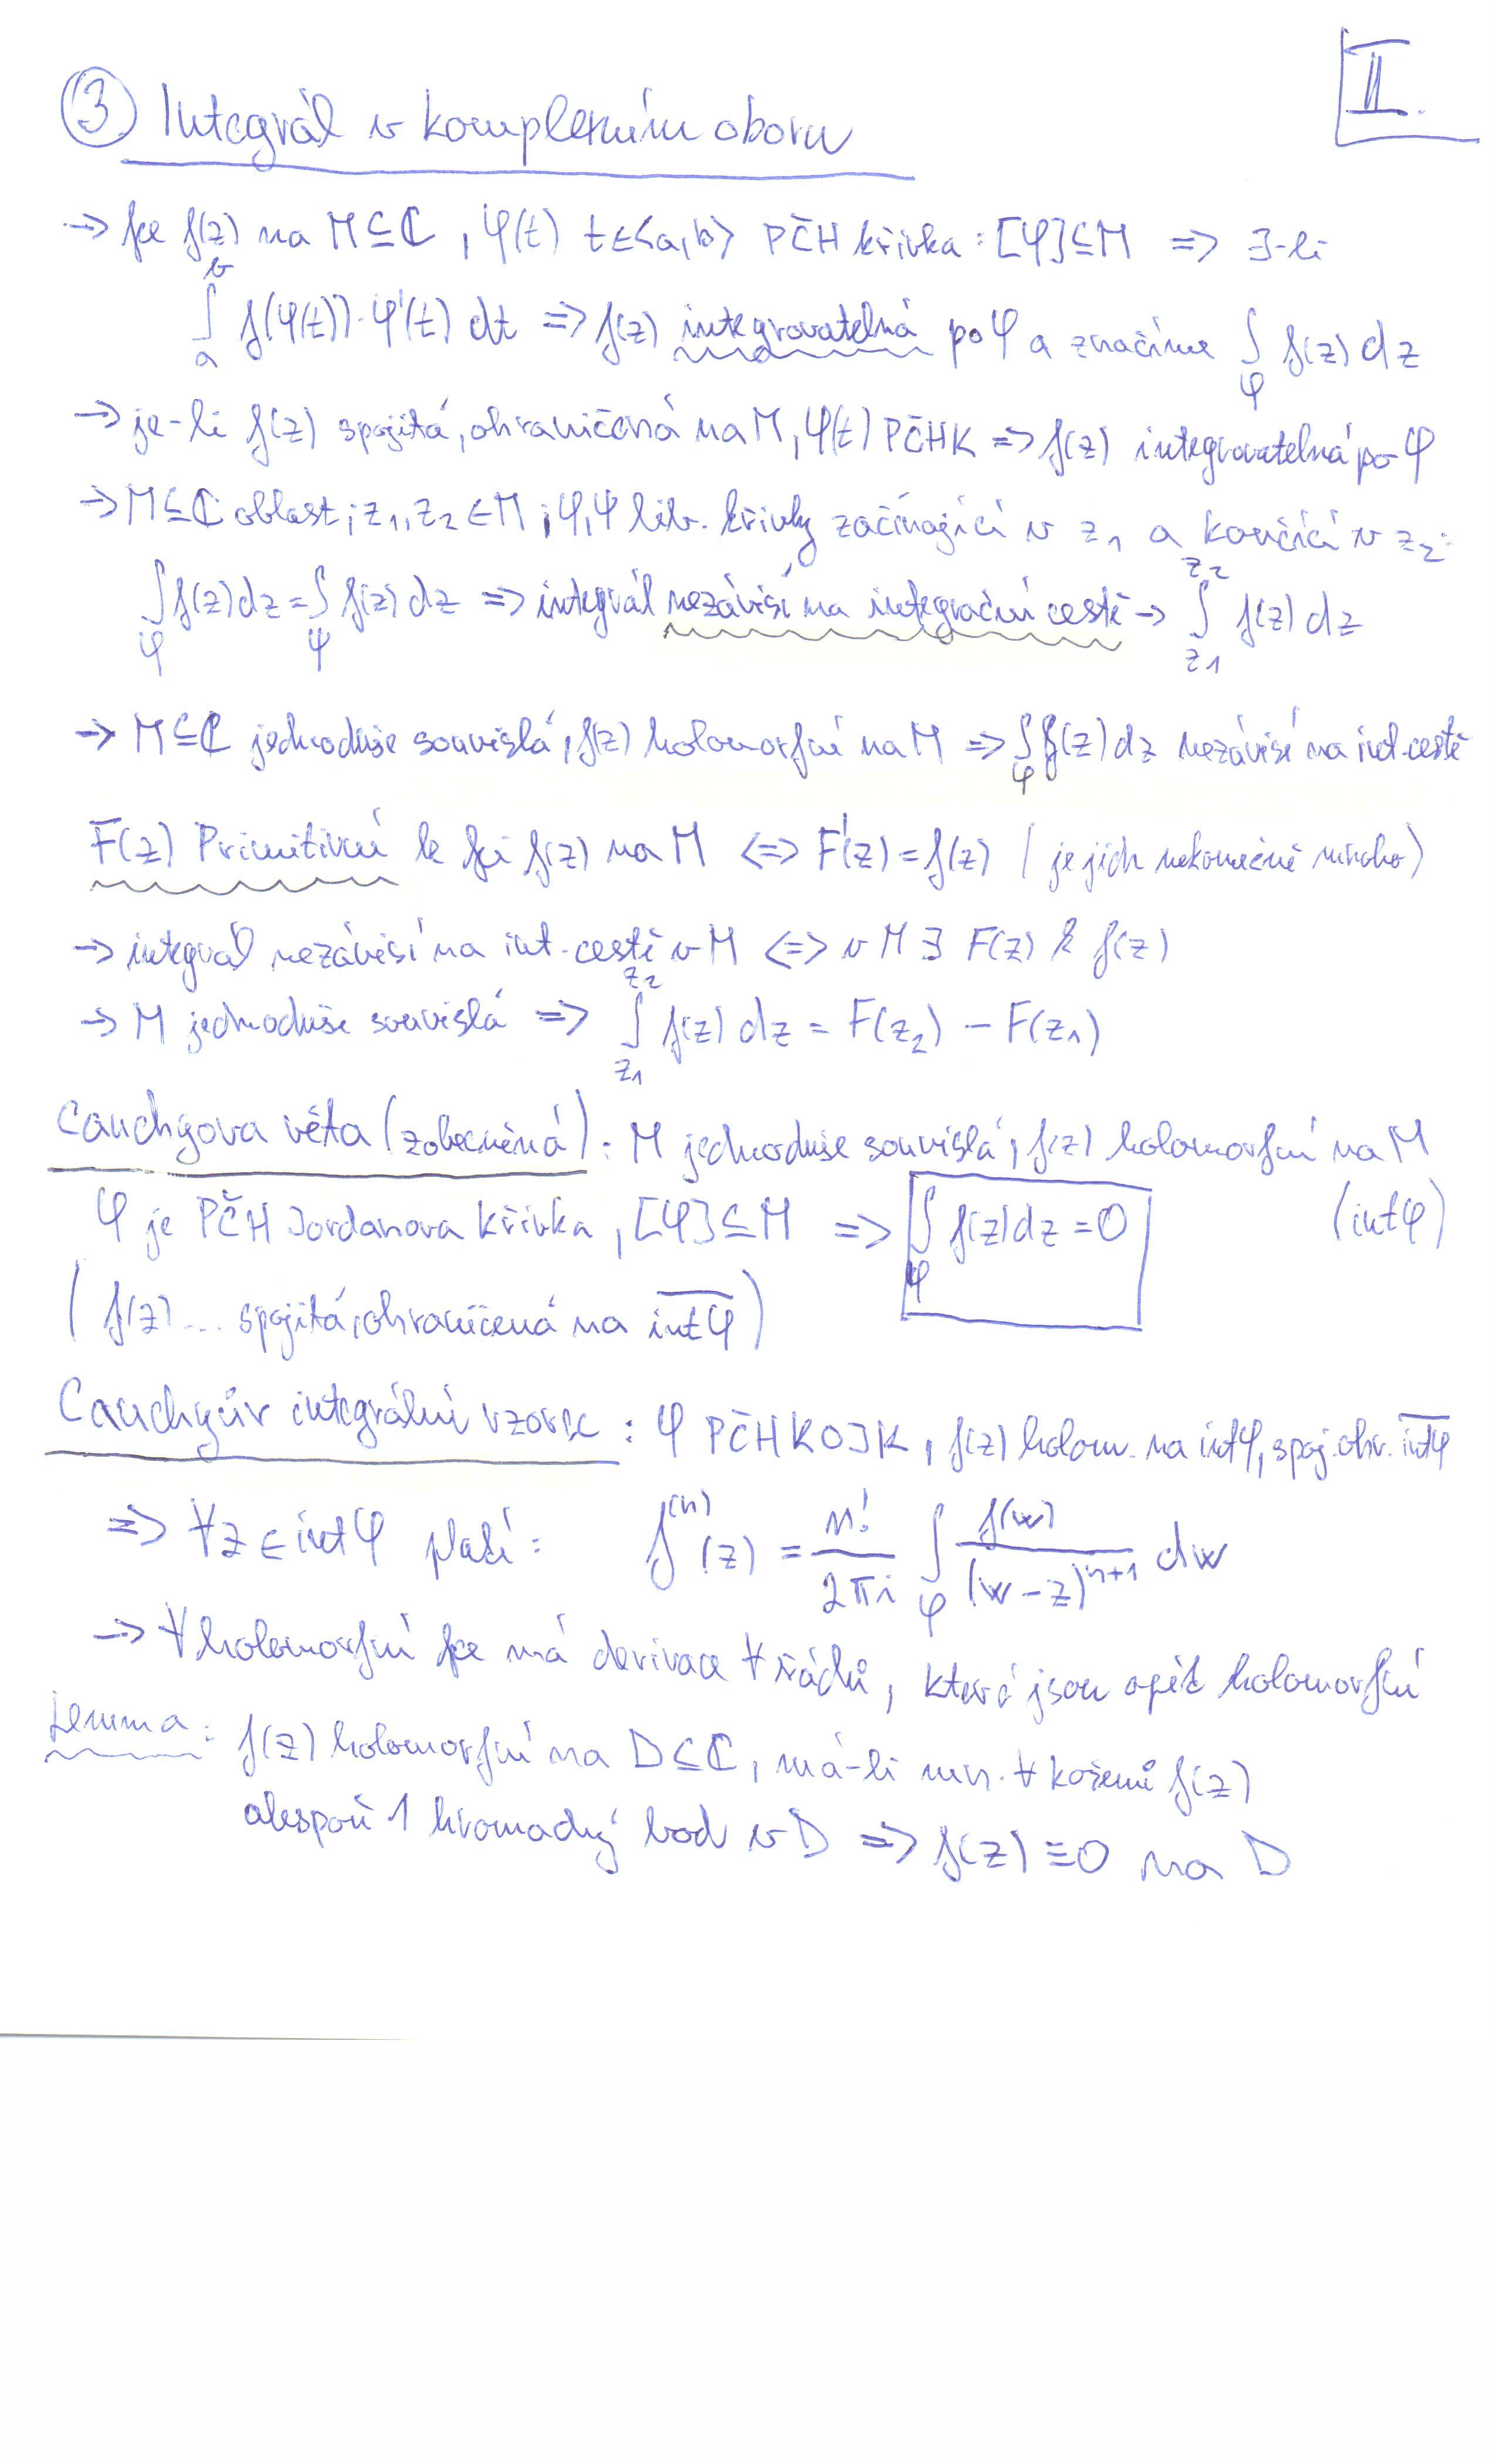
\includegraphics[width=\textwidth]{2-3a.jpg}
%\end{figure}

%\begin{figure}[H]
%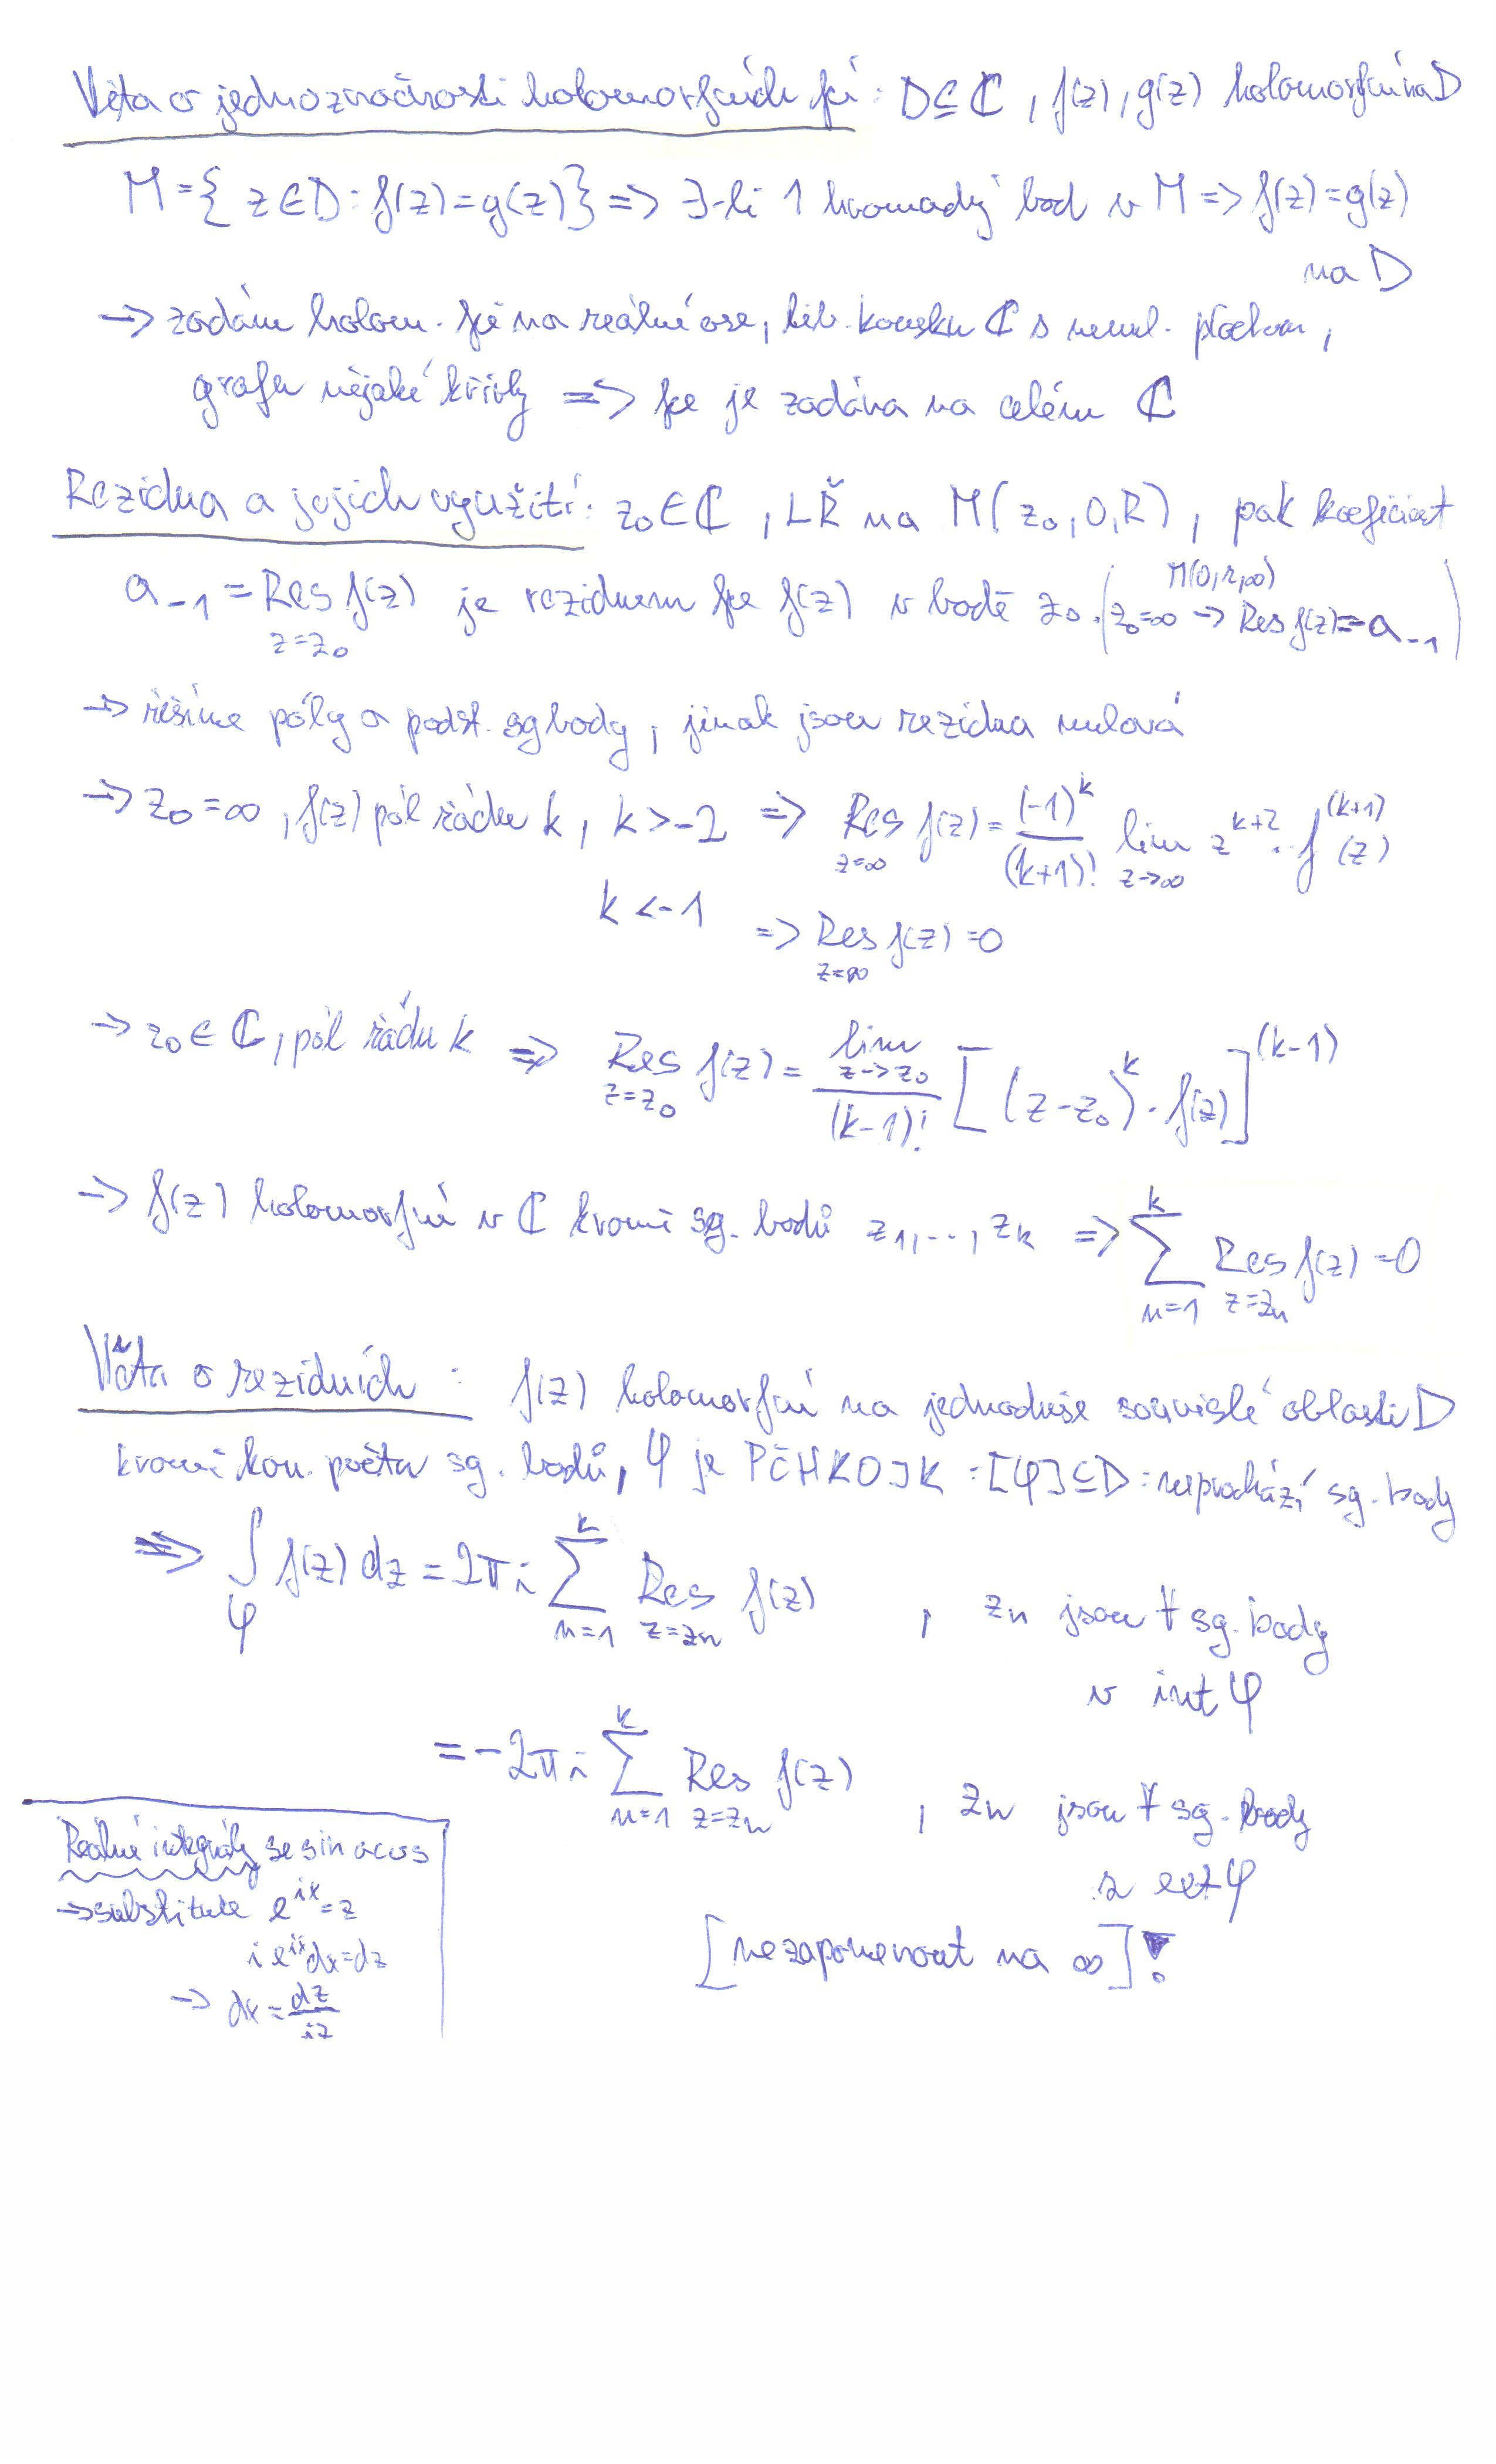
\includegraphics[width=\textwidth]{2-3b.jpg}
%\end{figure}


\section{Konformní zobrazení}
\subsection{Konformní zobrazení: věta o zachování úhlů, konformní ekvivalentnost oblastí, Riemannova věta}
\begin{definition}
	Nechť $M,N$ jsou otevřené množiny. Nechť $f:M\rightarrow N$ má následující vlastnosti:
	\begin{itemize}
		\item \fz je bijekce
		\item \fz je holomorfní
		\item $f'(z)\neq 0$ pro $\forall z \in M$
	\end{itemize}
\end{definition} 
Pak řekneme, že \fz je konformním zobrazením množiny $M$ na množinu $N$.

\begin{theorem}
	Nechť $\varphi$ a $\psi$ jsou dvě hladké křivky takové, že průnik jejich grafů $[\varphi] \cap [\psi]=\{z_0\}, z_0\in \CC $ a $z_0$ není počáteční, ani koncový bod grafů.
	Nechť $p$ je orientovaná tečna ke grafu $[\varphi]$ v bodě $z_0$ a $q$ je orientovaná tečna ke grafu $[\psi]$ v bodě $z_0$. Nechť \fz je holomorfní na okolí $O(z_0)$. Nechť $t$ je orientovaná tečna ke grafu $[f(\varphi)]$ v bodě $f(z_0)$ a s je orientovaná tečna ke grafu $[f(\psi)]$ v bodě $f(z_0).$ Nechť $f'(z_0) \neq 0$. Pak platí, že orientovaný úhel $\sphericalangle (p,q)=\sphericalangle (t,s)$   
\end{theorem}
%%%%%%%%%%%%%%%%%%%%%%%%%%%%%%%%%%%%%%%%%%%%%%%%%%%%%%%%%%%%%%

%%%%%%%%%%%%%%%%%%%%%%%%%%%%%%%%%%%%%%%%%%%%%%%%%%%%%%%%%%%%%%
\begin{definition}
	Řekneme, že dvě otevřené množiny $M,N \subseteq \CC$ jsou konformně ekvivalentní $(M\sim_K N)$, existuje-li mezi nimi konformní zobrazení.
\end{definition}

\begin{theorem}
	Nechť $M,N, K \subseteq \CC$ jsou otevřené množiny potom platí
	\begin{itemize}
		\item $f(z)=z$ je konformní zobrazení $M$ na $M$
		\item Je-li $f:M\rightarrow N$ konformní zobrazení, pak $f^{-1}: N\rightarrow M$ je konformní zobrazení $N$ na $M$.
		\item $f:M\rightarrow N$ je konformní zobrazení a $g:N\rightarrow K$ je konformní zobrazení $N$ na $K$, pak funkce $g \circ f:M\rightarrow K$ je konformní zobrazení $M$ na $K$.
	\end{itemize}
\end{theorem}

\begin{theorem}
	\textbf{Riemannova věta:} Nechť $M,N$ jsou dvě jednoduše souvislé oblasti, které jsou vlastními podmnožinami $\CC, (M,N \subset \CC) $ pak $N\sim_K M$
\end{theorem}

\begin{theorem}
	Neexistuje jiná množina od $\CC$ pro kterou platí $M\sim_K \CC$, tj. $\CC $ není konformně ekvivalentní s~žádnou vlastní podmnožinou.
\end{theorem}

\begin{theorem}
	Nechť $M\subseteq \CC$ je k-násobně souvislá oblast. Nechť $N \subseteq \CC $ je l-násobně souvislá oblast a nechť platí, že $M\sim_K N$. Pak $k=l$.
\end{theorem}


%\begin{figure}[H]
%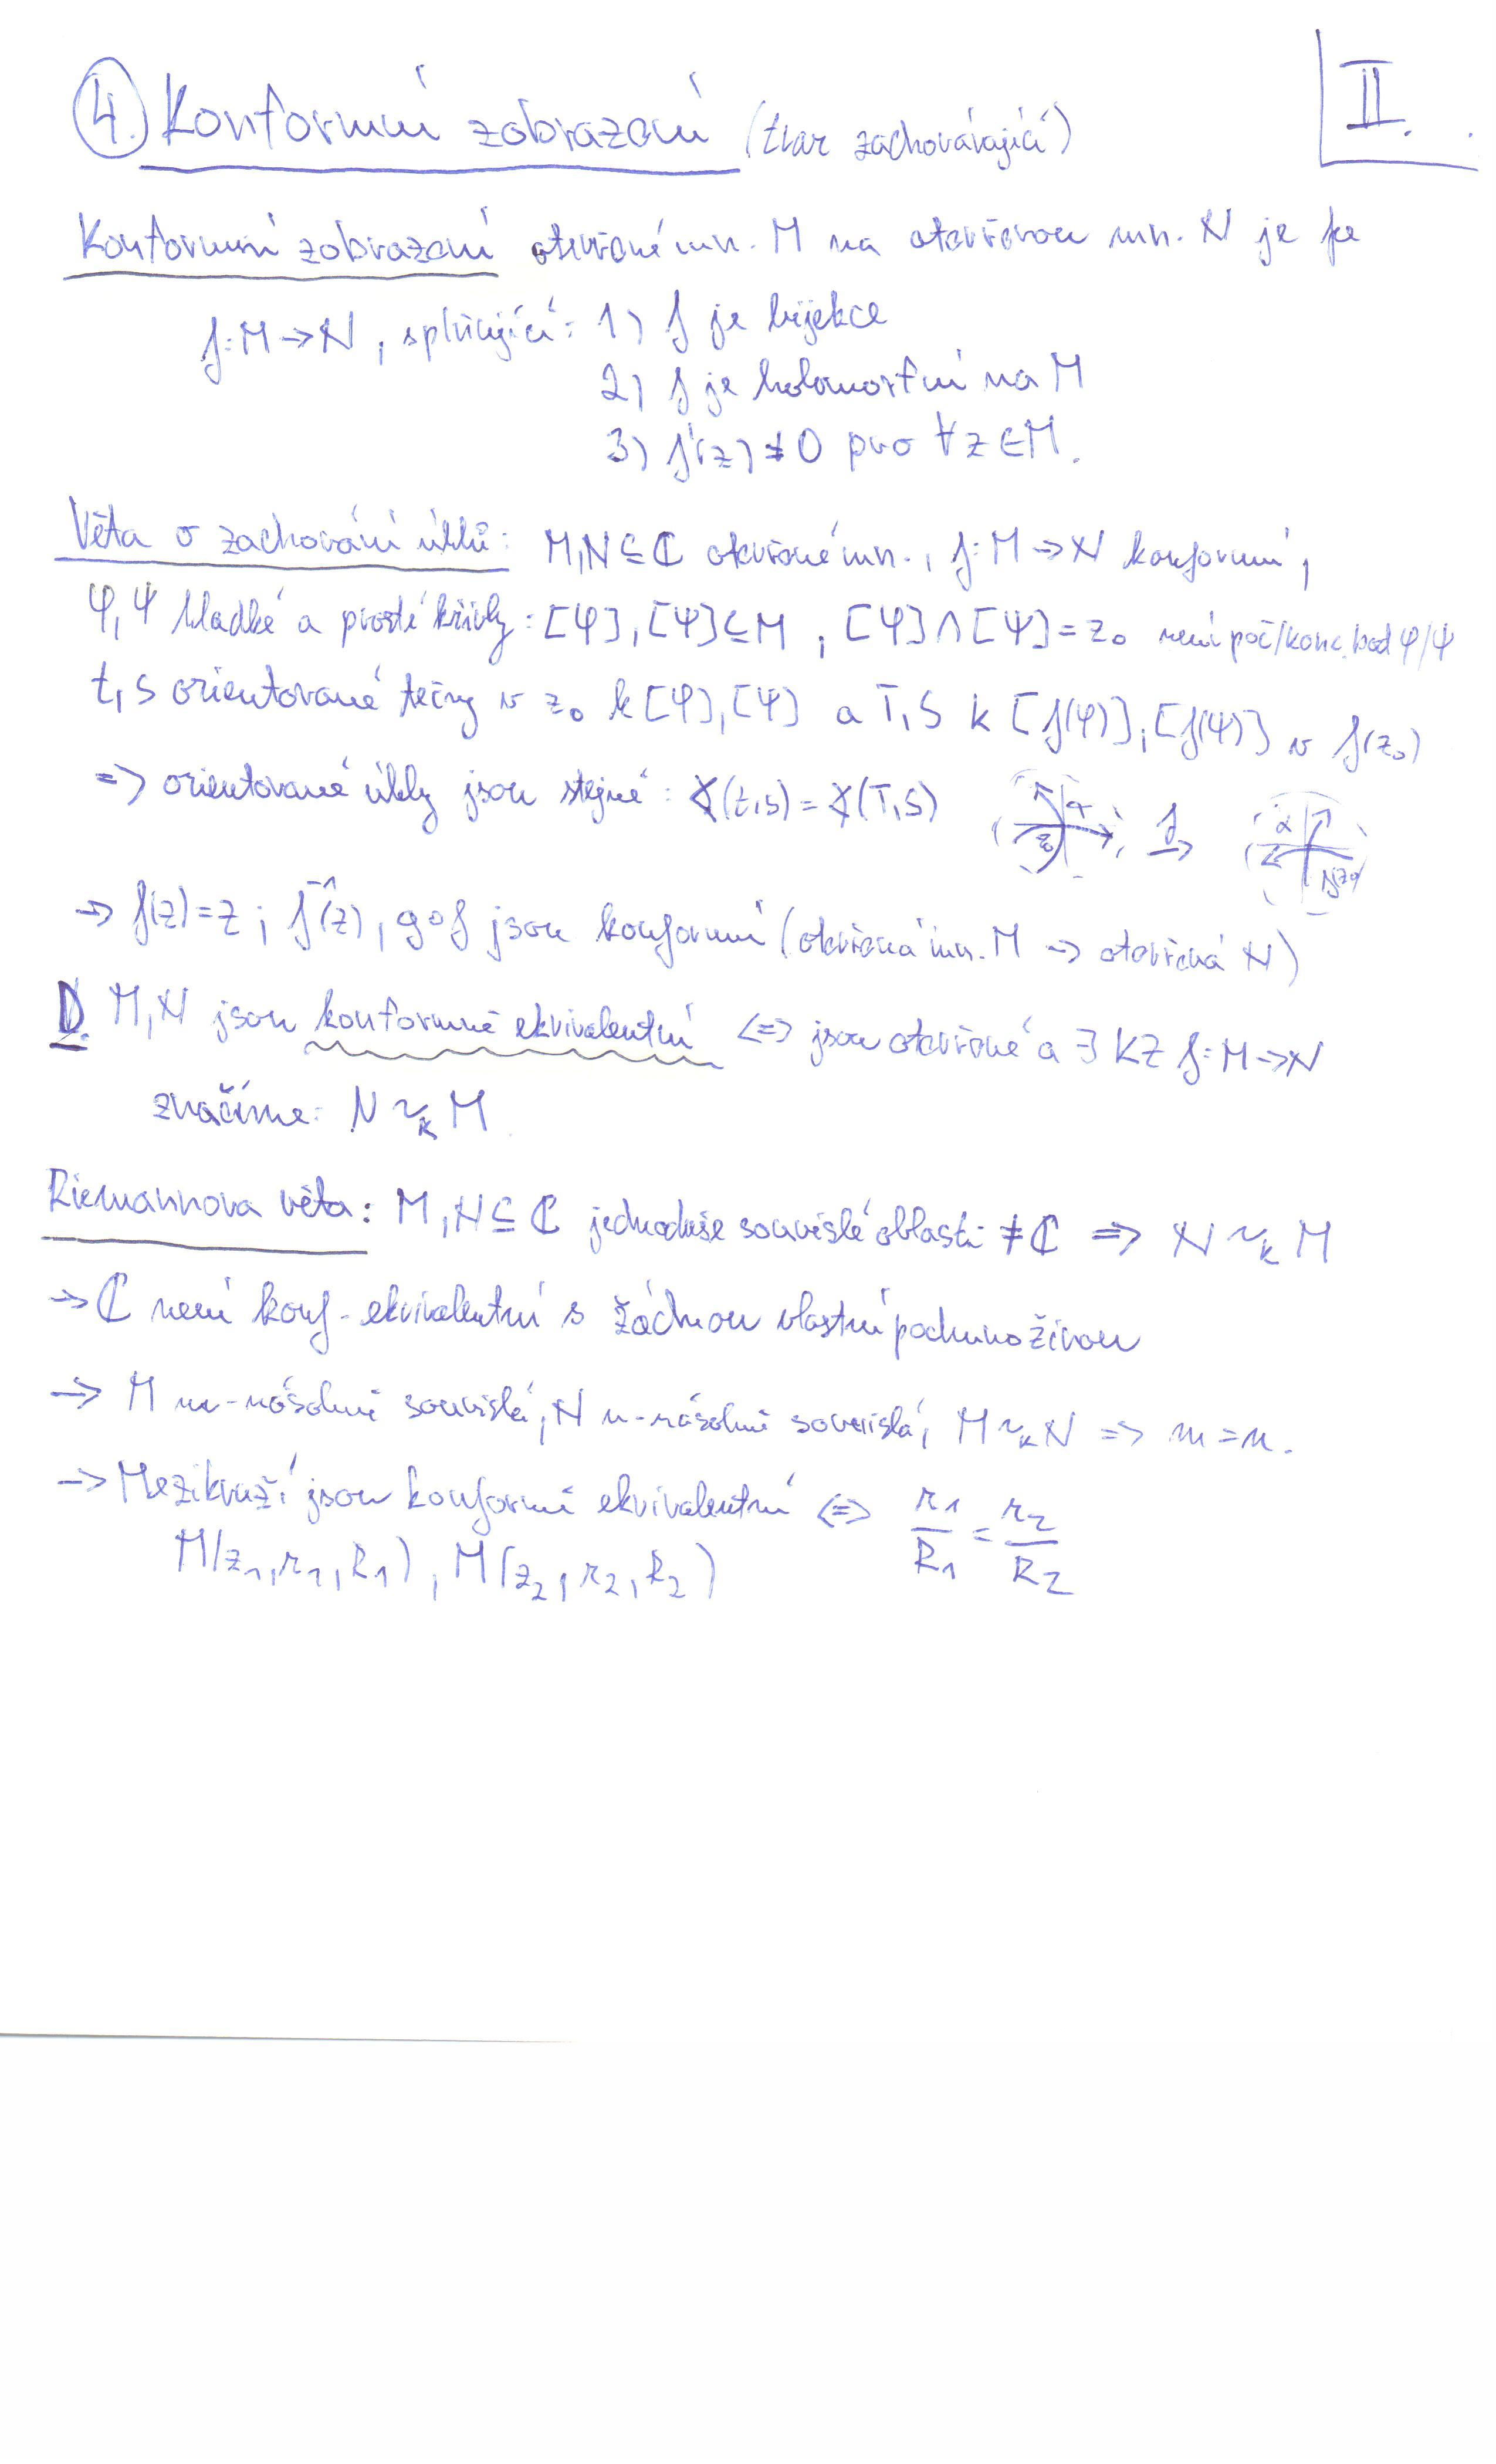
\includegraphics[width=\textwidth]{2-4a.jpg}
%\end{figure}

%\begin{figure}[H]
%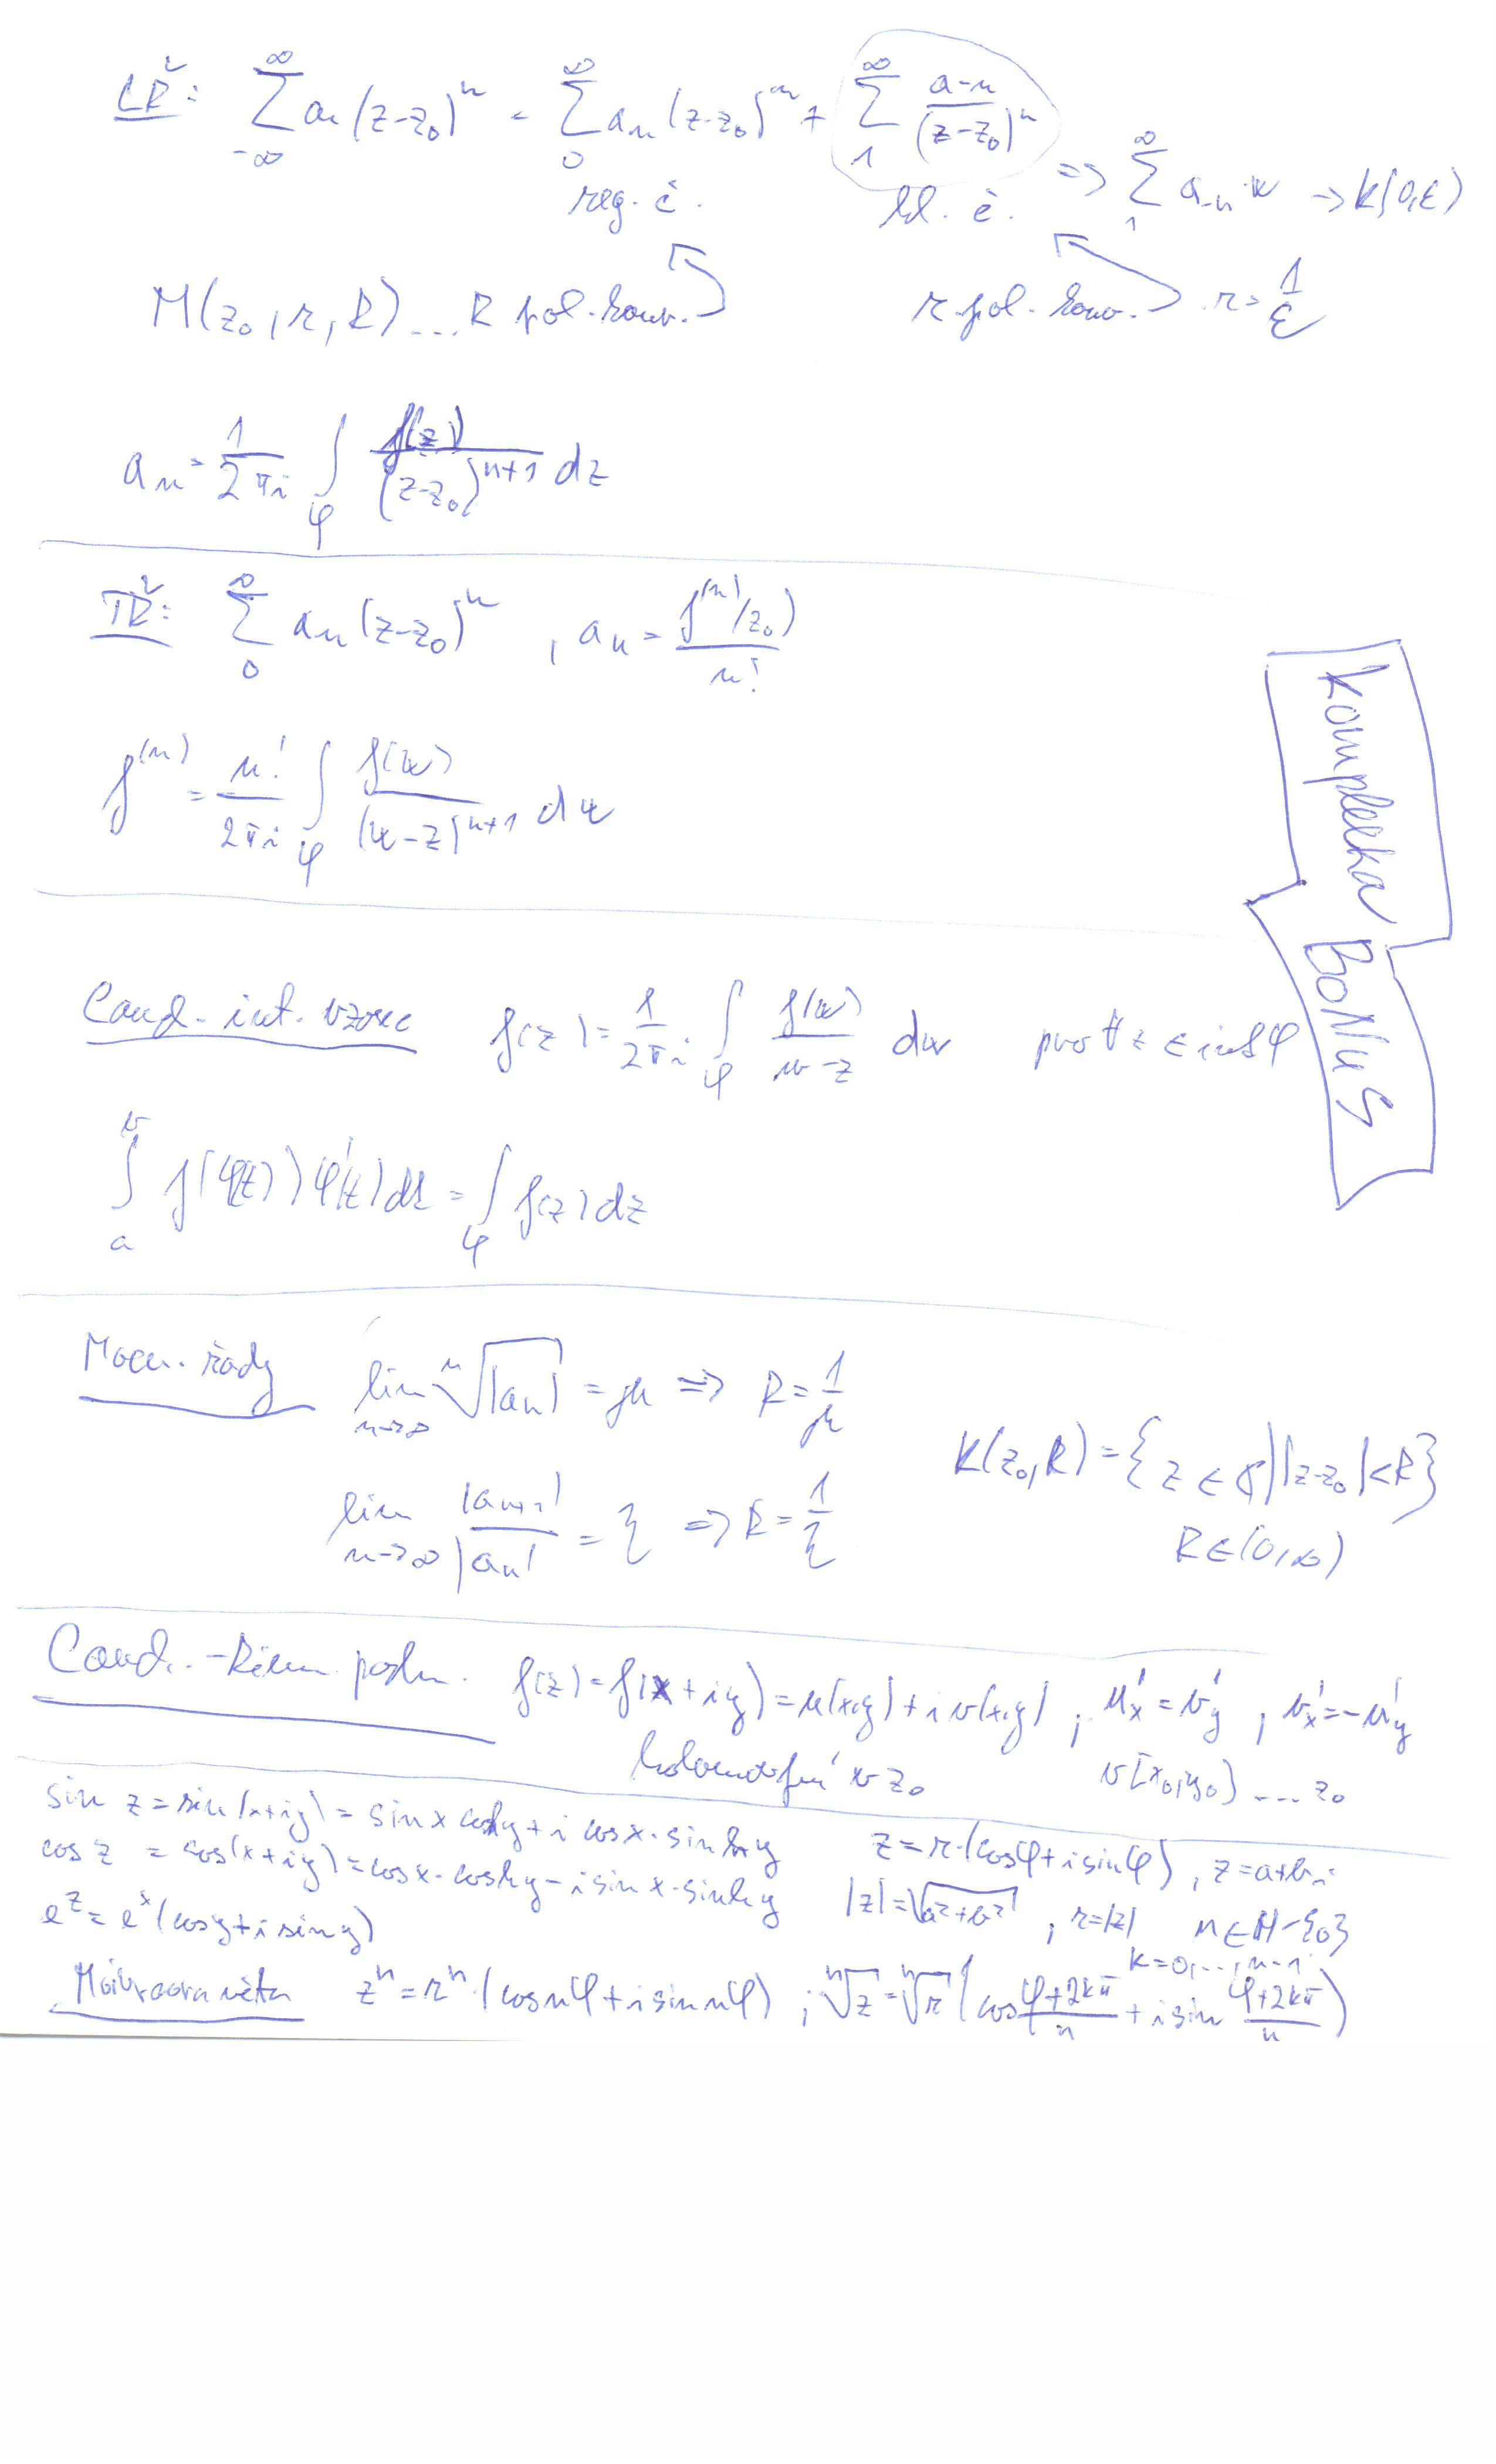
\includegraphics[width=\textwidth]{2-4b.jpg}
%\end{figure}

\begin{figure}[H]
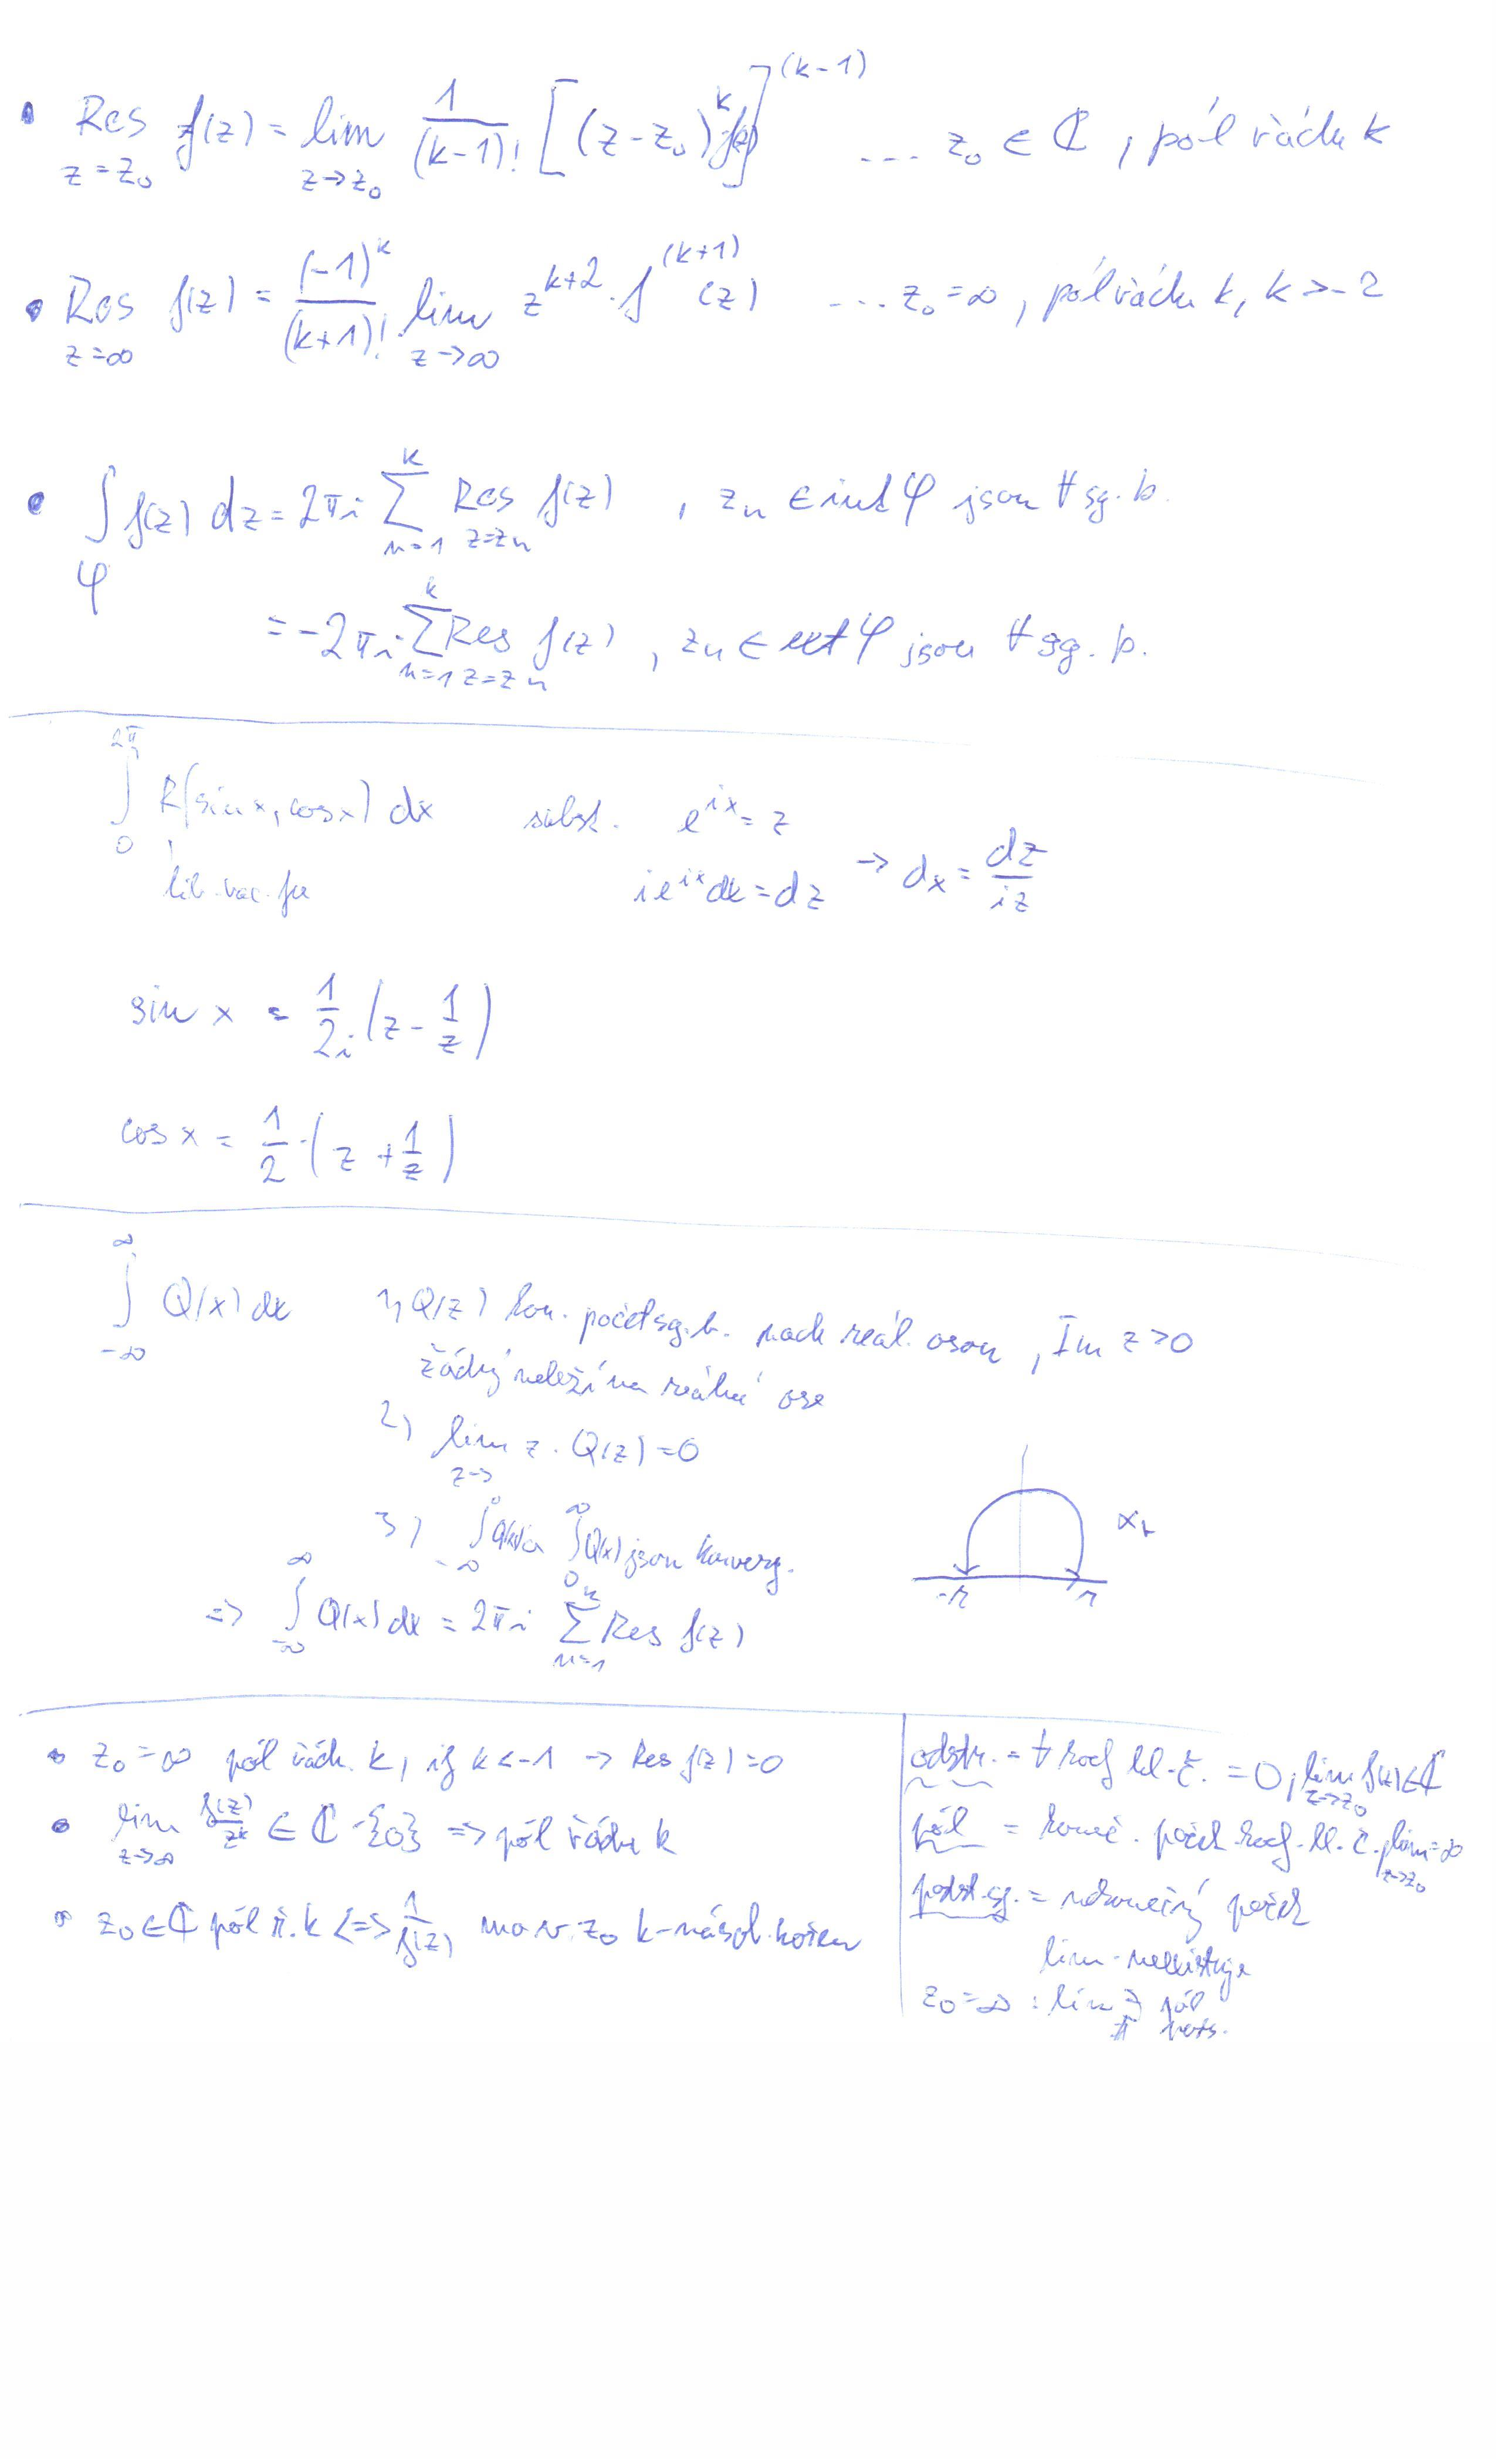
\includegraphics[width=\textwidth]{Obrazky/2-4c.jpg}
\end{figure}

\begin{figure}[H]
\section{Klasická teorie PDR}
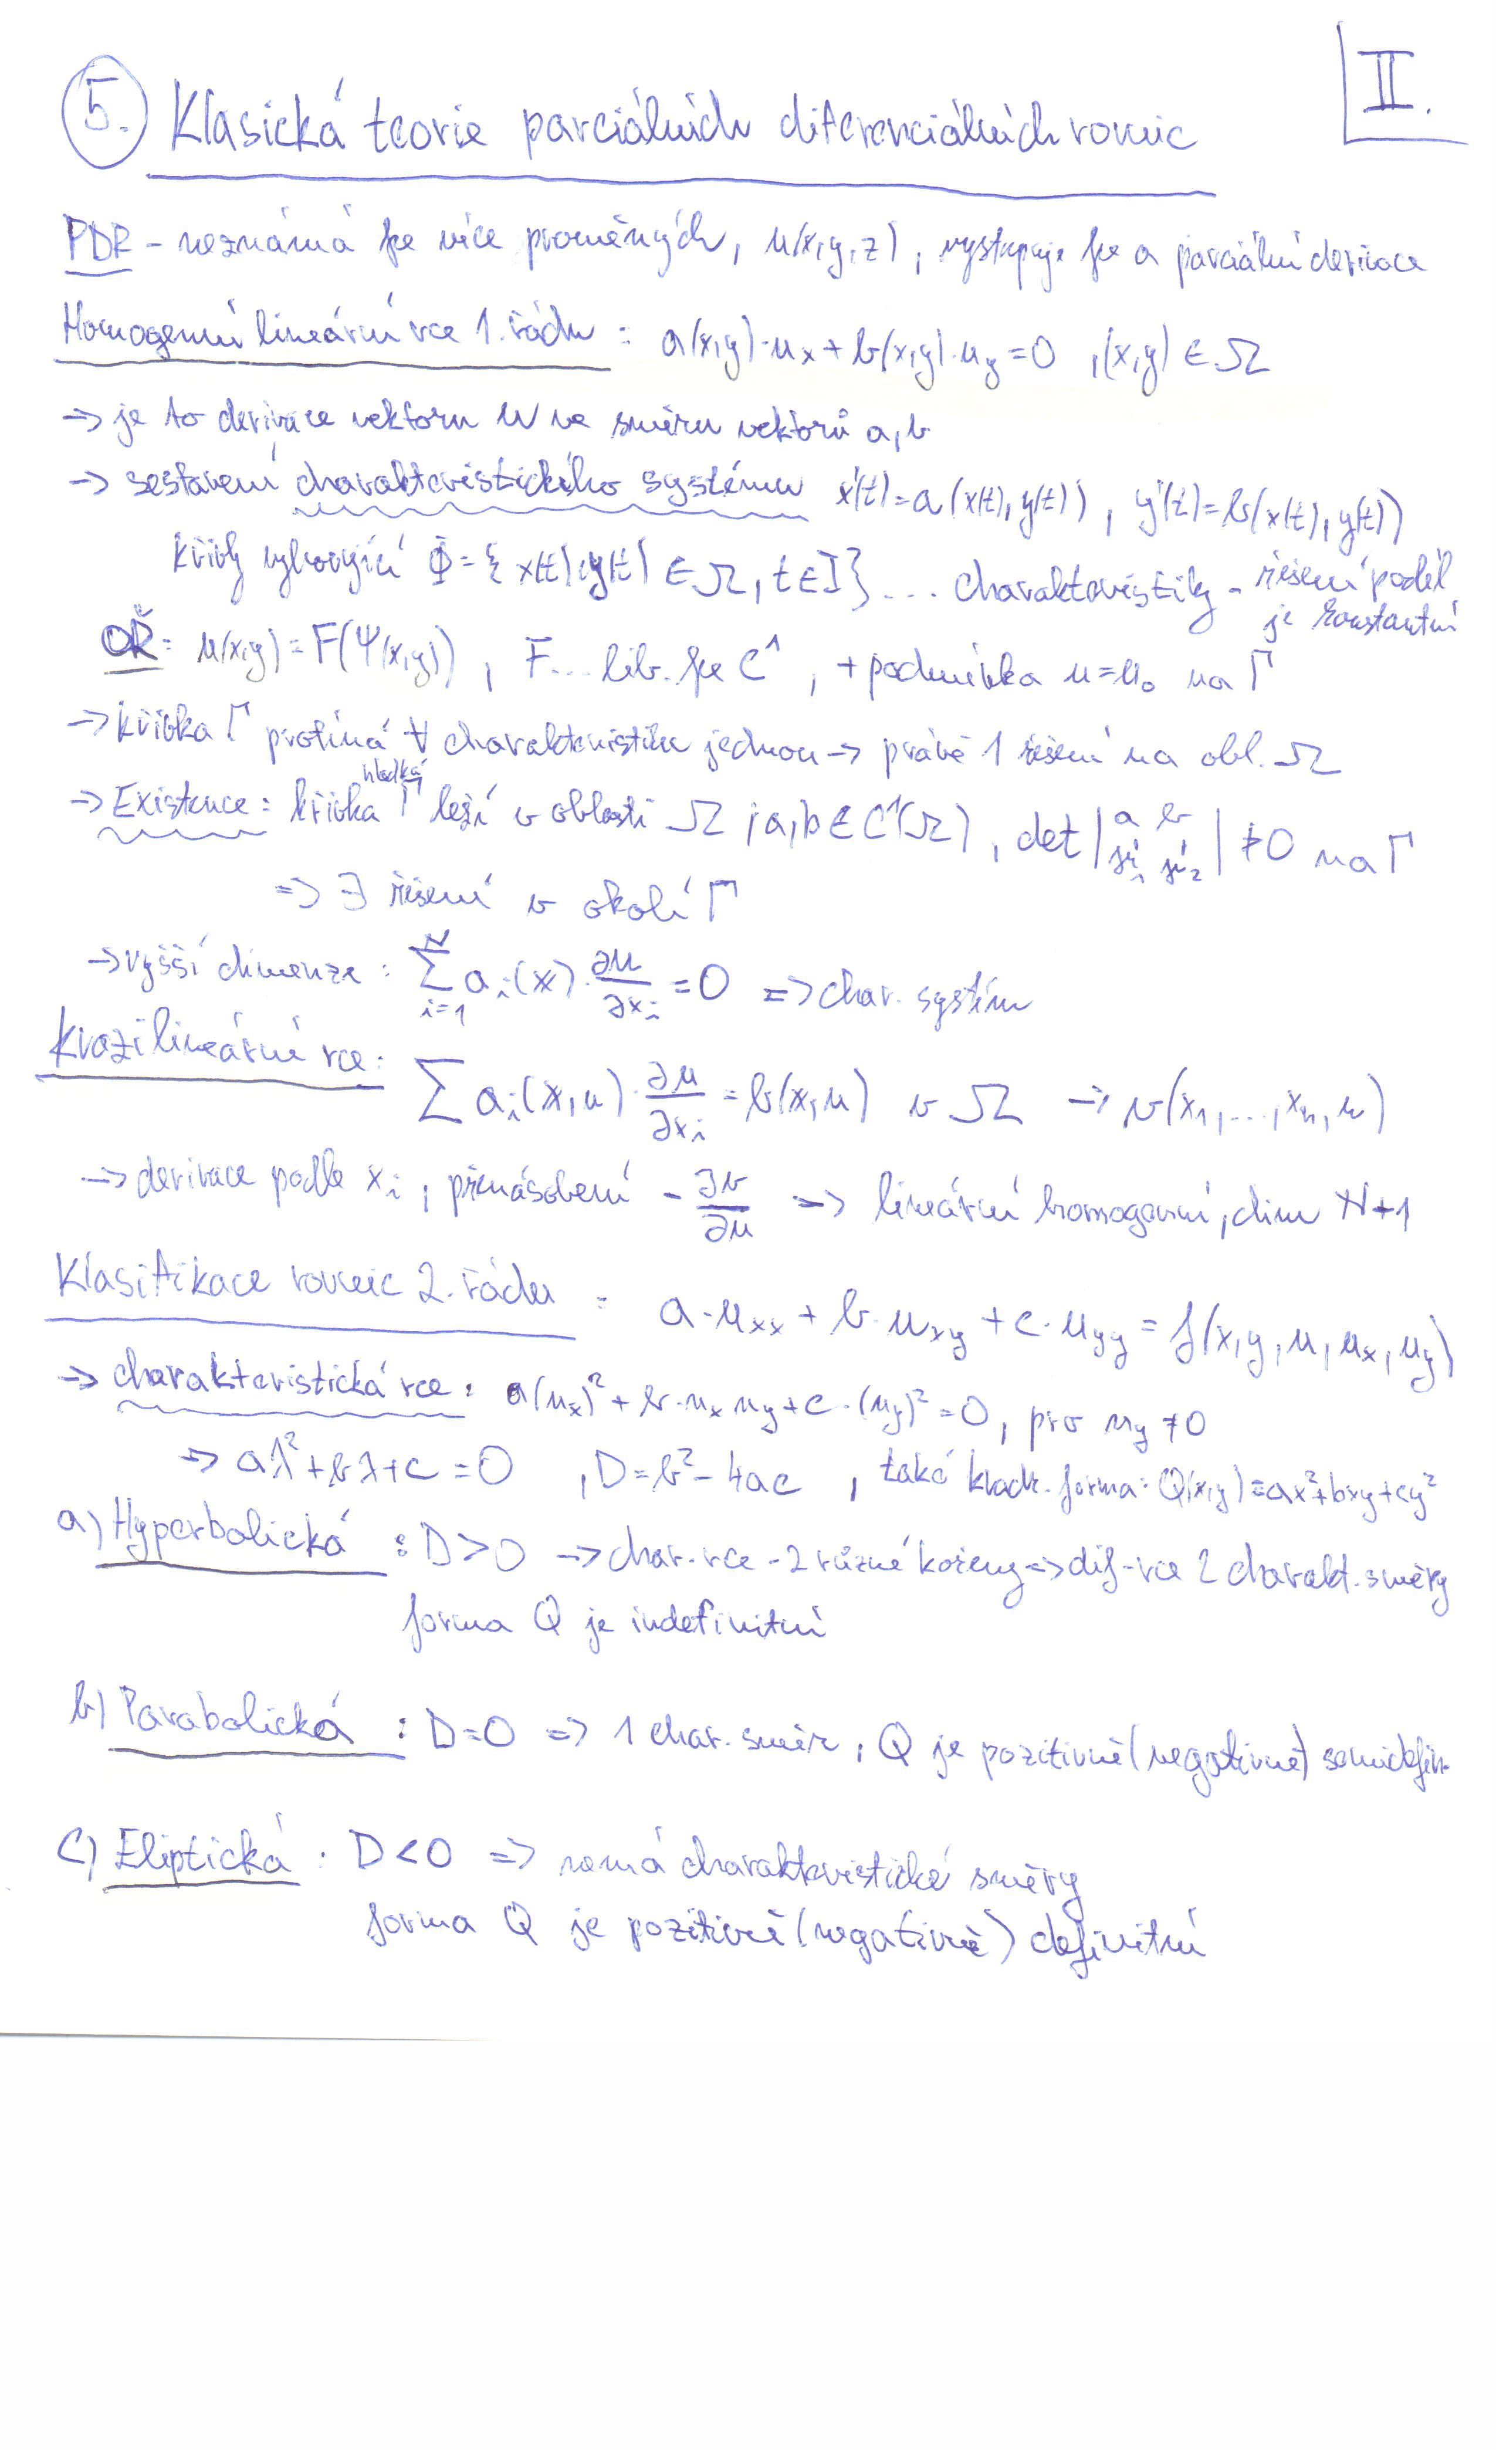
\includegraphics[width=\textwidth]{Obrazky/2-5a.jpg}
\end{figure}

\begin{figure}[H]
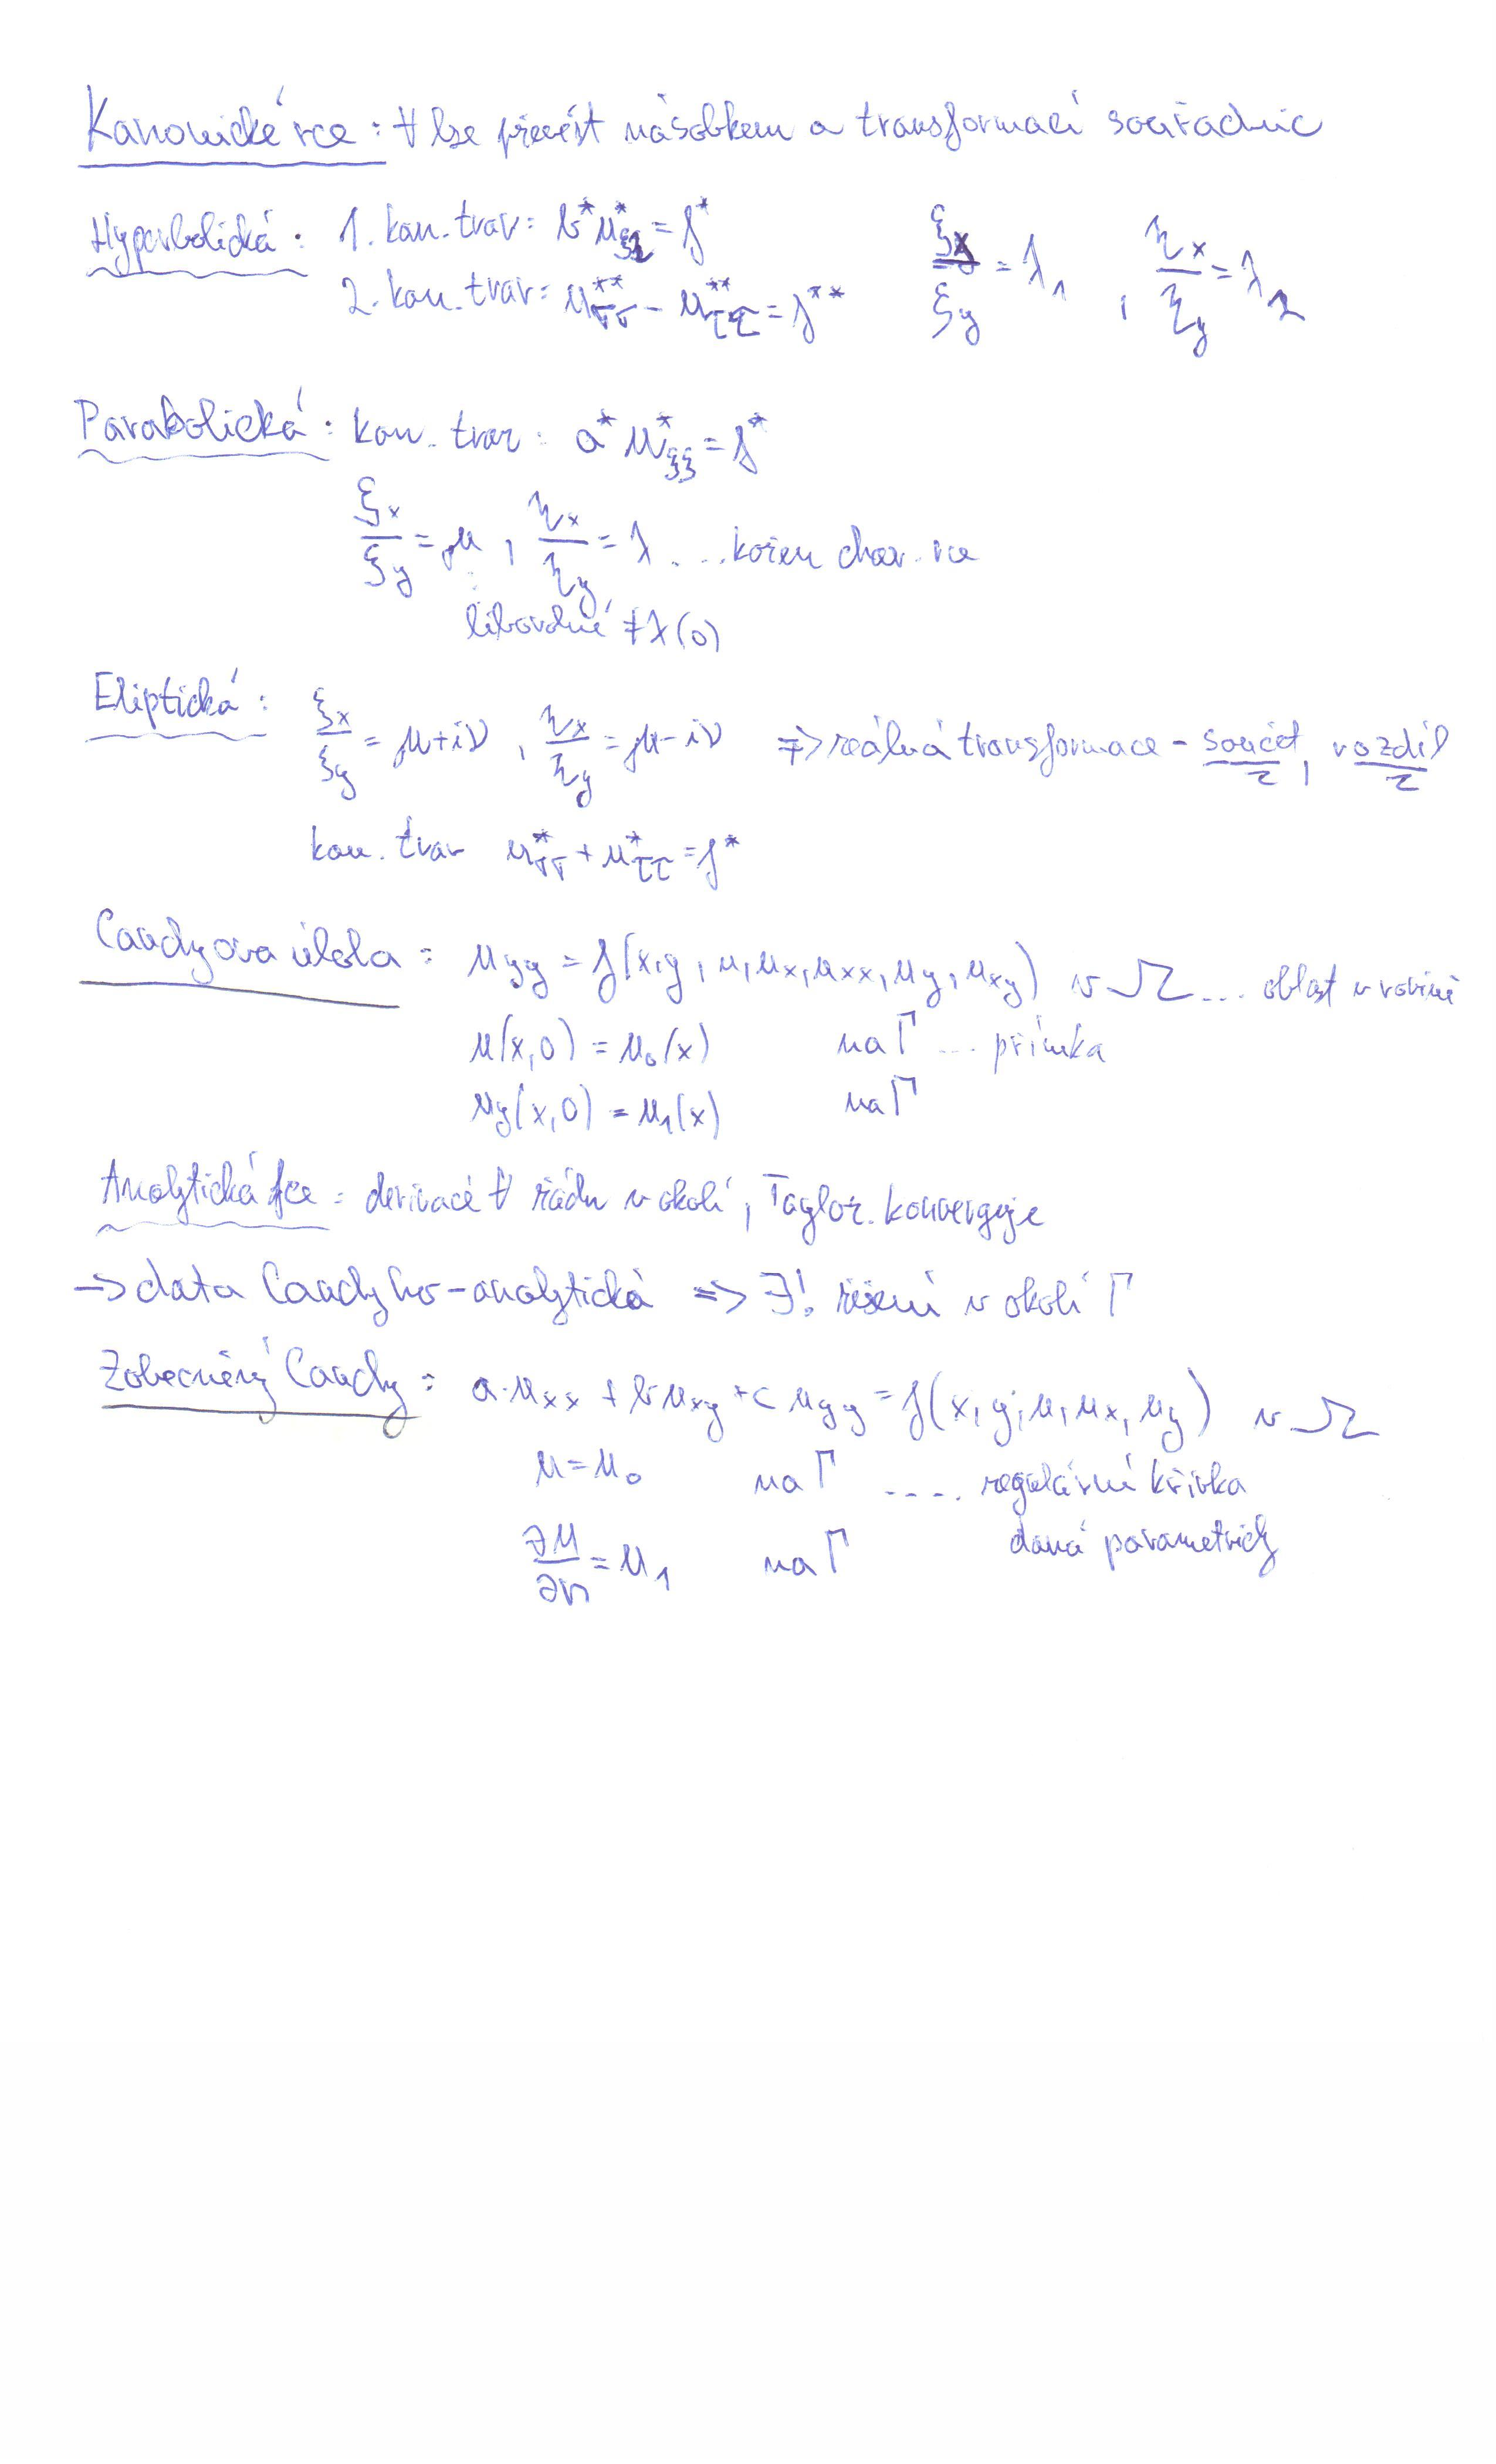
\includegraphics[width=\textwidth]{Obrazky/2-5b.jpg}
\end{figure}

\begin{figure}[H]
\section{Řešení PDR 2}
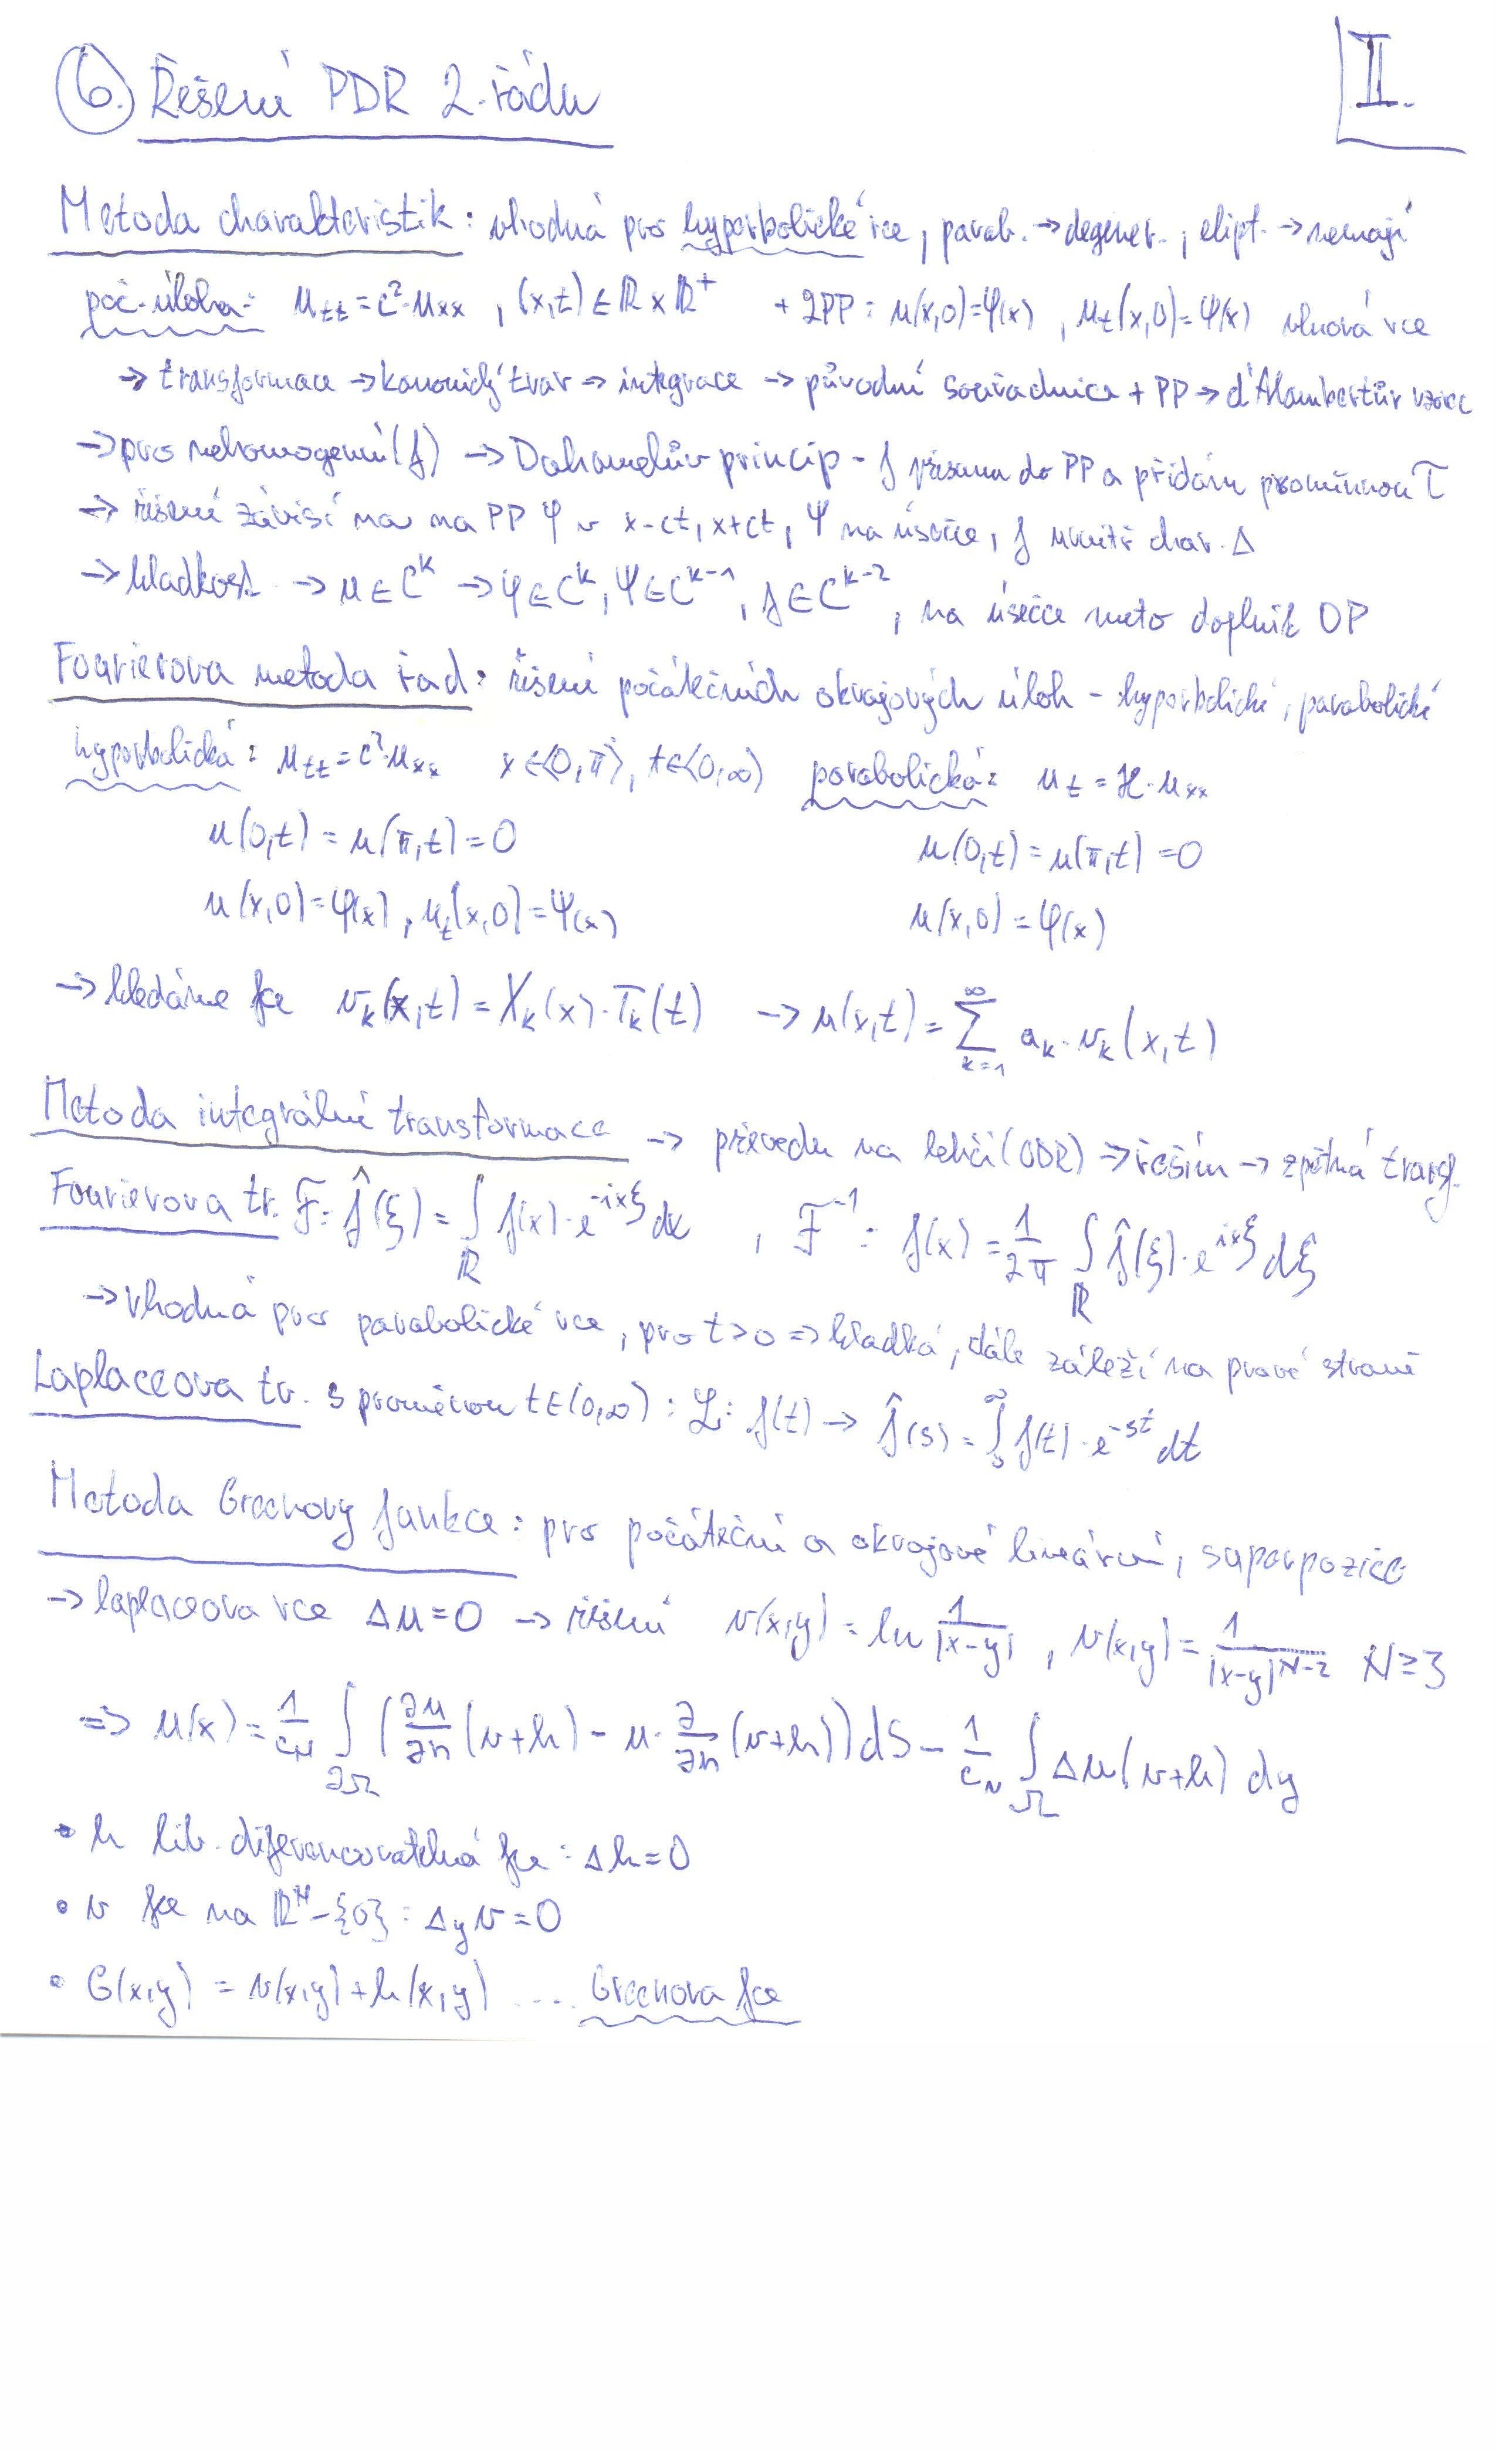
\includegraphics[width=\textwidth]{Obrazky/2-6a.jpg}
\end{figure}

\begin{figure}[H]
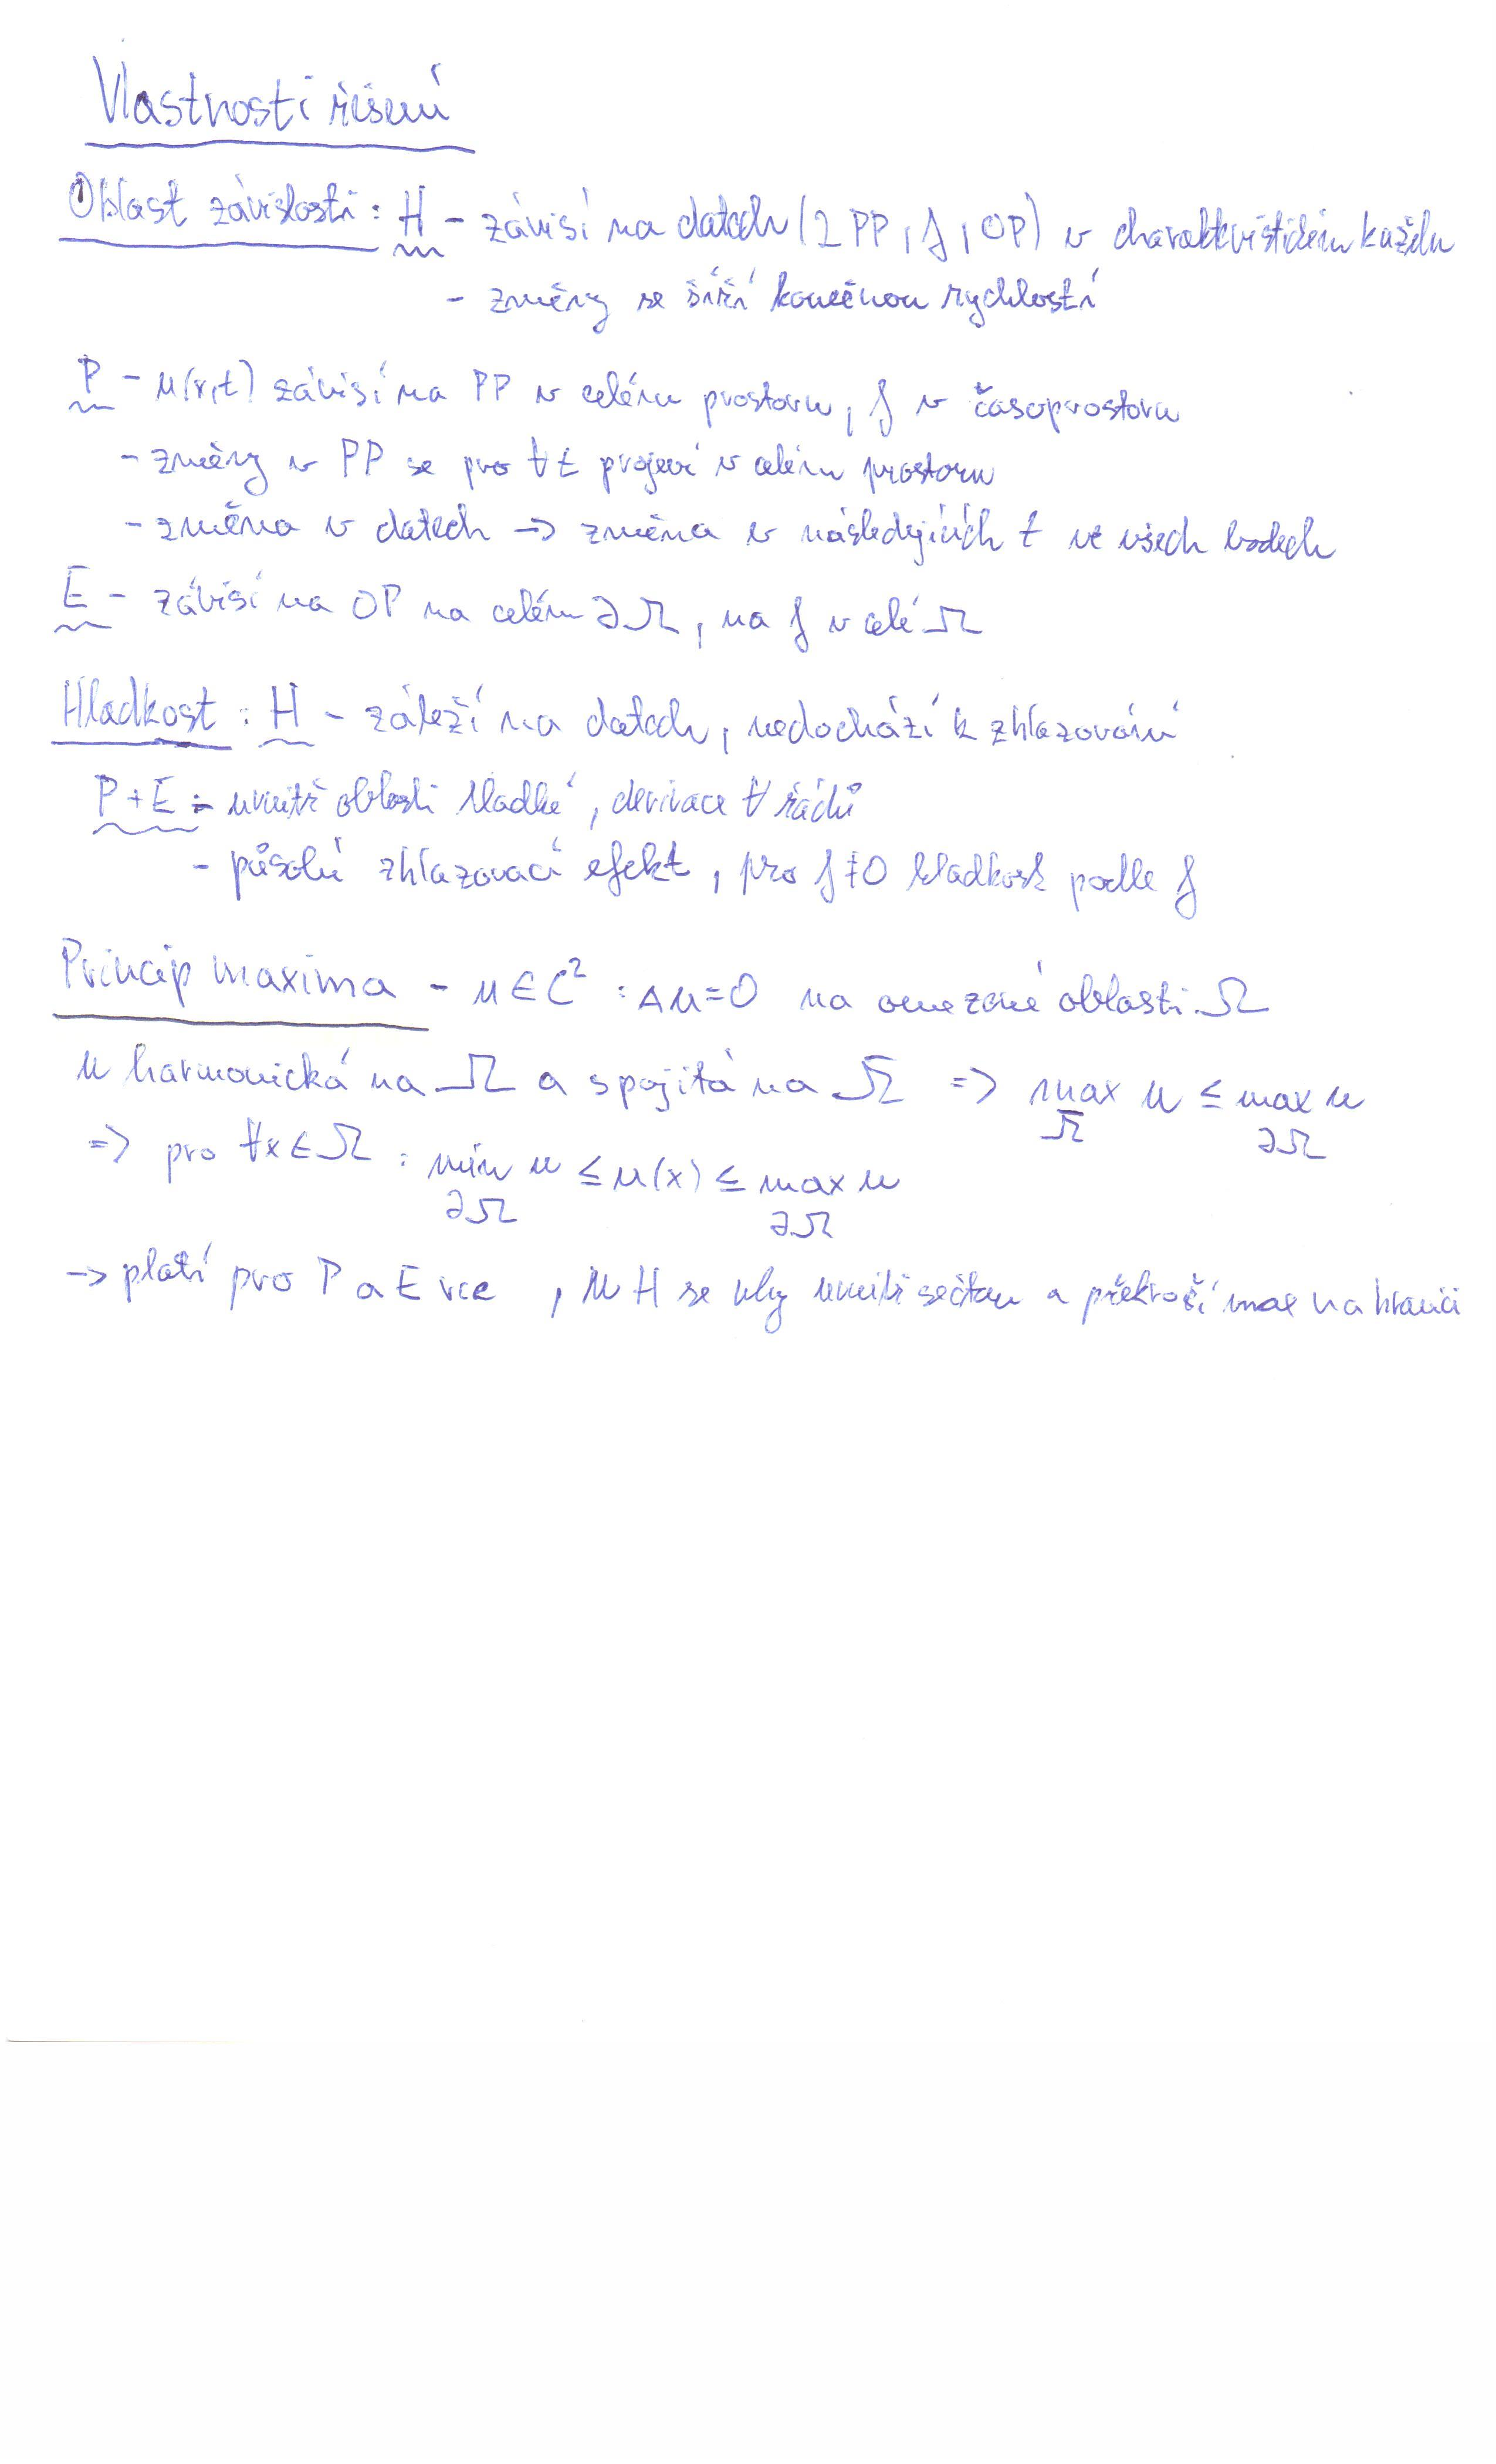
\includegraphics[width=\textwidth]{Obrazky/2-6b.jpg}
\end{figure}


\section{Rovnice matematické fyziky}

\subsection{Přehled}
\begin{itemize}
    \item Parabolická
        \begin{itemize}
            \item $\Omega \subset \mathbb{R}^N$, $I=(t_0,\infty)$
            \item $u_t=\Delta u +f$\ \ \ \ na $\Omega\times I$
            \item (PP) $u(x,t_0)=u_0(x)$\ \ \ \ na $\Omega$
            \item (OP) $\alpha \frac{\partial u}{\partial n} +\beta u=g$\ \ \ \ na $\partial\Omega\times I$
            \item vedení tepla ($u$=teplota, $N=1$ pro tyč, $N=2$ pro desku, $N=3$ pro těleso)
        \end{itemize}
    \item Hyperbolická
        \begin{itemize}
            \item $\Omega \subset \mathbb{R}^N$, $I=(t_0,\infty)$
            \item $u_{tt}=\Delta u +f$\ \ \ \ na $\Omega\times I$
            \item (1.PP) $u(x,t_0)=u_0(x)$\ \ \ \ na $\Omega$
            \item (2.PP) $u_t(x,t_0)=u_1(x)$\ \ \ \ na $\Omega$
            \item (OP) $\alpha \frac{\partial u}{\partial n} +\beta u=g$\ \ \ \ na $\partial\Omega\times I$
            \item kmitání, vlnění ($u$=odchylka, $N=1$ pro příčné, podélné kmity, $N=2$ pro kmitání membrány, bubliny, $N=3$ pro akustické, elektro-magnetické vlny)
        \end{itemize}    
    \item Eliptická
        \begin{itemize}
            \item $\Omega \subset \mathbb{R}^N$
            \item $\Delta u=f$\ \ \ \ na $\Omega$
            \item (PP) $u(x,t_0)=u_0(x)$\ \ \ \ na $\Omega$
            \item (OP) $\alpha \frac{\partial u}{\partial n} +\beta u=g$\ \ \ \ na $\partial\Omega$
            \item ustálený stav předchozích, Poissonova rovnice (při $f=0$ Laplaceova rovnice, vedení elektrického proudu, Airyho funkce napětí,   )
        \end{itemize}  
\end{itemize}

\subsection{Rovnice vedení tepla v tyči}

Nejjednodušším případem vedení tepla je vedení tepla v tenké tyči. Označením tenká tyč myslíme tyč s takovým průřezem, jenž je vzhledem k délce zanedbatelný a v němž jsou všechny uvažované veličiny konstantní.

Zavádíme souřadnici $x$, jenž popisuje tyč podélně a čas $t$. Funkce, která bude v diferenciální rovnici vystupovat jako neznámá, bude $T(x,t)$, což je teplota tyče v okamžiku $t$ a poloze $x$. Předpokládáme, že je tyčka na povrchu izolovaná, abychom mohli zanedbat ztráty teploty do okolí, což ovšem neznamená absolutní oddělení tyčky a okolí (vnější zdroj energie). 

Nyní budeme pracovat s elementem tyčky $(x_a,x_b)$ a elementem času $(t_\alpha, t_\beta)$.

Zavedeme veličinu $Q_a$ (resp. $Q_b$), která říká, jak velké množství tepla vyteče z elementu ven přes konec $x_a$ (resp. $x_b$) během časového intervalu $(t_\alpha,t_\beta)$. Veličina $Q_f$ \mbox{popisuje} množství tepla, které do úseku $(x_a,x_b)$ dodáme během $(t_\alpha,t_\beta)$ zvnějšku (předpo\-kládáme tedy nějaký vnější zdroj tepla působící na tyčku). Dále si rozepíšeme \mbox{jednotlivé} protékající tepla.

\begin{equation}
Q_a =-\int_{t_\alpha}^{t_\beta} q(x_a,t) dt,   
\end{equation}

\begin{equation}
Q_b =\int_{t_\alpha}^{t_\beta} q(x_b,t) dt,   
\end{equation}

\begin{equation}
Q_f =\int_{x_a}^{x_b} \int_{t_\alpha}^{t_\beta} f(x,t) dt dx  ,
\end{equation}

kde funkcí $q(x,t)$ myslíme tepelný tok a funkcí $f(x,t)$ myslíme hustotu výkonu tepelného zdroje.

Uděláme tepelnou bilanci, čimž myslíme souhrn všech tepel, které se v úseku vyskytují. Veličinou $\Delta Q$ myslíme teplo, které po časovém úseku v úseku tyčky zůstalo. Tepelnou bilanci děláme s ohledem na zákon zachování energie. Tuto veličinu si zrovna vyjádříme pomocí funkce $e(x,t)$, která vyjadřuje hustotu vnitřní energie.

\begin{equation}
\Delta Q = Q_f - Q_a -Q_b, 
\end{equation}

\begin{equation}
\Delta Q =\int_{x_a}^{x_b} e(x,t_\beta) dx    -\int_{x_a}^{x_b}  e(x,t_\alpha)dx. 
\end{equation}

Nyní tyto dvě vyjádření $\Delta Q$ dáme do rovnosti a upravíme. Následující úpravy předpokládají potřebné derivace a spojité prostředí.

\begin{equation}
\int_{x_a}^{x_b} e(x,t_\beta)dx-\int_{x_a}^{x_b}  e(x,t_\alpha)dx= \int_{x_a}^{x_b} \int_{t_\alpha}^{t_\beta} f(x,t) dt dx+\int_{t_\alpha}^{t_\beta} q(x_a,t) dt-\int_{t_\alpha}^{t_\beta} q(x_b,t) dt, 
\end{equation}

\begin{equation}
\int_{x_a}^{x_b} \int_{t_\alpha}^{t_\beta} \frac{\partial e}{\partial t} (x,t) dt
dx= \int_{x_a}^{x_b} \int_{t_\alpha}^{t_\beta} f(x,t)-\frac{\partial q}{\partial x} (x,t)dt dx,
\end{equation}

\begin{equation}
\int_{x_a}^{x_b} \int_{t_\alpha}^{t_\beta} \frac{\partial e}{\partial t}(x,t)-f(x,t)+\frac{\partial q}{\partial x} (x,t) dt dx=0 ,
\end{equation}

\begin{equation}
\lim_{x_b\rightarrow x_a} \lim_{t_\beta \rightarrow t_\alpha} \frac{1}{x_b-x_a}\frac{1}{t_\beta-t_\alpha}\int_{x_a}^{x_b} \int_{t_\alpha}^{t_\beta} \frac{\partial e}{\partial t}(x,t)-f(x,t)+\frac{\partial q}{\partial x} (x,t) dt
dx=0 ,
\end{equation}

\begin{equation}    
\frac{\partial e}{\partial t}(x,t)-f(x,t)+\frac{\partial q}{\partial x} (x,t)=0.\label{hxbwkuehbkuwhfcuwkbfwhck} \end{equation}

Doposud bylo odvozování přesné. V dalším přesnost mírně ztratíme z důvodu použití vztahů mezi energií/tepelným tokem a teplotou. 
Dále si funkce výše uvedené upravíme pomocí jiných veličin (konstituční vztahy).
\begin{equation}
e(x,t)=\overline{e}(x,T(x,t))=C(x)T(x,t)+K,
\end{equation}
kde $C(x)$ je množství tepla, které je nutno dodat do jednotkové délky tyče, aby se teplota zvýšila o $1^o C$ (tedy měrná tepelná kapacita neboli měrné teplo), a $K$ je konstanta která při derivování vypadne.
\begin{equation}
\frac{\partial e}{\partial t}=C(x) \frac{\partial T}{\partial t}(x,t)
\end{equation}

Tepelný tok upravíme podle Fourierova zákona vedení tepla (viz podkapitola 2.3) následovně:
\begin{equation}
q(x,t)=-\frac{\partial T}{\partial x}(x,t)\lambda(x),
\end{equation}
kde $\lambda(x)$ je tepelná vodivost a záporné znaménko je tam z důvodu toho, že teplo vždy teče z teplého na studené.

Pokud vše dosadíme do (\ref{hxbwkuehbkuwhfcuwkbfwhck}) dostáváme:

\begin{equation}
C(x) \frac{\partial T}{\partial t}=\frac{\partial }{\partial x} \bigg(\lambda(x)\frac{\partial T}{\partial x}(x,t)\bigg)+f(x,t).
\end{equation}
Dostali jsme tedy parciální diferenciální rovnici druhého řádu.

Měrná tepelná kapacita bývá vztažena většinou na jednotku hmotnosti a nikoli délky. Vztáhneme ji tedy na jednotku hmotnosti úpravou $\rho c(x)=C(x)$, kde $\rho$ je hustota materiálu. Všimněme si, že předpokládáme nezávislost $c(x)$ a $\lambda(x)$ na teplotě. Pokud by hodnoty těchto dvou veličin byly nezávislé i na $x$ a tyčka tedy byla z homogenního materiálu, mohli bychom s nimi zacházet jako s čísly a diferenciální rovnice by vypadala: 

\begin{equation} T^\prime_t=\frac{\lambda}{ c\rho} T^{\prime\prime}_{xx}+\frac{f}{ c\rho}.
\end{equation}

K jednoznačnému řešení úlohy vedení tepla v tyči ovšem ještě potřebujeme počáteční podmínku v čase $t_0$ (v případě tyčky konečné délky následující platí pro $x\in (a,b)$ a v případě tyče nekonečné délky $x\in \mathbb{R}$).
\begin{equation} 
T(x,t_0)=T_0 (x).
\end{equation}

To by stačilo v případě nekonečně dlouhé tyče. V případě tyče konečné délky je ještě potřeba dodat okrajové podmínky, které mohou být vícero druhu. První uvedeme Dirichletovy podmínky, které říkají, jaká teplota je na okrajích tyčky.
\begin{equation}
T(x_a,t)=T_a(t), \ \ \ \ \ 
T(x_b,t)=T_b(t),  \ \ \ \ \   t>t_0.
\end{equation}
Dalším typem okrajových podmínek jsou Neumannovy okrajové podmínky, které předepisují tepelný tok na okrajích.
\begin{equation}
T^\prime_x(x_a,t)=g_a(t),  \ \ \ \ \
T^\prime_x(x_b,t)=g_b(t), \ \ \ \ \      t>t_0.
\end{equation}
Posledním typem jsou Robinovy okrajové podmínky, které jsou kombinací prvních dvou. V následujícím musí být $\alpha$ a $\beta$ větší než nula, protože jinak by se jednalo \mbox{o předchozí} podmínky.
\begin{equation}
-\alpha_a T^\prime_x(x_a,t)+\beta_a T(x_a,t)=g_a(t), \ \ \ \ \
\alpha_b T^\prime_x(x_b,t)+\beta_b T(x_b,t)=g_b(t),\ \ \ \ \   t>t_0.
\end{equation}

Diferenciální rovnice popsaná v předešlém je \textbf{parabolického} typu.

\subsection{Rovnice vedení tepla v tělese}
Tuto rovnici zde uvedeme bez odvození a pouze s popisem okrajových podmínek a jednoho konstitučního vztahu týkajícího se Fourierova zákona. Teplota je značena jako $T(x_1,x_2,t)$. Měrná tepelná kapacita je značena jako $c(x_1,x_2)$. Tepelný tok je značen jako $\mathbf{\dot{q}}(x_1,x_2)$. Hustota materiálu je $\rho (x_1,x_2)$ a hustota vnitřního zdroje je značena $f(x_1,x_2)$.

\begin{equation}
c \rho T_t^\prime+div(\mathbf{\dot{q}})-f=0 .
\end{equation}

Úprava tepelného toku lze rozdělit na více případů zavisejících na druhu materiálu.
\begin{itemize}
\item Izotropní materiál:
$\dot{q}_i=-\lambda\frac{\partial T}{\partial x_i}$, kde $\lambda$ je tepelná vodivost.
\item Anizotropní materiál v hlavních směrech:\\
$\dot{q}_i=-\lambda_i \frac{\partial T}{\partial x_i}$, kde $\lambda_i$ je tepelná vodivost ve směru $i$.
\item Anizotropní materiál obecně:\\
$\dot{q}_i=-\sum_{j=1}^{3} \lambda_{ij}\frac{\partial T}{\partial x_j}$, kde $\lambda_{ij}$ je symetrická matice tepelných vodivostí.
\end{itemize}

Uvedeme zde nyní parciální diferenciální rovnici popisující vedení tepla v izotropním tělese.
\begin{equation}
c \rho T_t^\prime=\lambda\Delta T +f\ .
\label{diferencialnirovnicepopisujicivednitepla}    
\end{equation}
 Opět je nutné uvést počáteční a případně i okrajové podmínky. Pokud se úloha týká celého prostoru, potom $\Omega = \mathbb{R}^3$:
\begin{equation}
T(\mathbf{x},t_0)=T_0(\mathbf{x}),\ \ \ \mathbf{x}\in\Omega,\ t>t_0.
\label{pocatecnipodminkapopisujicivednitepla}   
\end{equation}
Pokud je těleso konečných rozměrů, tak je potřeba dodat okrajové podmínky, \mbox{kterých} je opět vícero druhů:
\begin{itemize}

\item Dirichletovy OP: $T(\mathbf{x},t)=T_0(\mathbf{x},t), \ \ \ \ \mathbf{x}\in \partial\Omega $
\item Neumannovy OP: $ \frac{\partial T}{\partial n}(\mathbf{x},t)=g(\mathbf{x},t),  \ \ \ \ \mathbf{x}\in \partial\Omega      $

\item Robinovy OP: $ \frac{\partial T}{\partial n}(\mathbf{x},t)=-k_0 [T(\mathbf{x},t)-g(\mathbf{x},t) ],\ \ \ \ \mathbf{x}\in\partial\Omega$

\end{itemize}

Počáteční problém pro těleso s konečnými rozměry je tedy dán (\ref{diferencialnirovnicepopisujicivednitepla}), (\ref{pocatecnipodminkapopisujicivednitepla}) a některou z okrajových podmínek.

Diferenciální rovnice popsaná v předešlém je \textbf{parabolického} typu.

\subsection{Rovnice kmitání struny}
 Provedeme silovou bilanci úseku struny $(x_a,x_b)$ v čase $t$. Neznámou funkcí je $u(x,t)$, což značí kolmou výchylku struny v čase $t$ a místě $x$. Síla, kterou je struna napjatá, je $T$. Uvažujeme pohyb ve směru osy $y$. Pohyb ve směru osy $x$ zanedbáme. Předpokládáme tenkou strunu, v čemž se skrývá zanedbání odporu struny vůči ohýbání. Kmity předpokládáme "malé" a proto zanedbáme rozdíl mezi $sin \ \alpha$ a $tg \ \alpha$.
 
 Pro úsek struny $(x_a,x_b)$ v čase $t$ provedeme bilanci průmětů do osy $y$ sil působících na tento úsek.
 $$F_a, F_b=\textrm{průměty sil, kterými působí zbytek struny na úsek v jeho koncích }x_a,x_b $$
 $$F_f=\textrm{průměty známé vnější síly, například gravitace }$$
 
 Hlavní myšlenkou silové bilance bude Newtonův zákon. Výslednice sil působících na strunu je součinem hmotnosti a zrychlení. Jako celkovou sílu působící na úsek budeme označovat $F$. Funkce $f(x,t)$ charakterizuje vliv zdroje v místě $x$ a čase $t$. Úhel, který svírá struna a osa $x$, je značen v bodě $x_a$ jako $\alpha$ a v bodě $x_b$ jako $\beta$.

\begin{equation}
F_f=\int_{x_a}^{x_b} f(x,t)\ dx
\end{equation}
\begin{equation}
F_b=T sin \ \beta \doteq T tg\ \beta=T u_x (x_b,t)
\end{equation}
\begin{equation}
F_a=-T sin \ \alpha \doteq -T tg\ \alpha=-T u_x (x_a,t)
\end{equation}
\begin{equation}
F=\int_{x_a}^{x_b} \rho u_{tt}(x,t)\ dx
\end{equation}
\begin{equation}
F_a+F_b+F_f=\int_{x_a}^{x_b}f(x,t)\ dx+T\bigg(u_x(x_b,t)-u_x(x_a,t)\bigg)
\end{equation}
\begin{equation}
u_x(x_b,t)-u_x(x_a,t)=\int_{x_a}^{x_b} \frac{\partial }{\partial x} u_x \ dx
\end{equation}
\begin{equation}
F=F_f+F_a+F_b
\end{equation}
\begin{equation}
\int_{x_a}^{x_b} \rho u_{tt}(x,t)\ dx=\int_{x_a}^{x_b} \bigg( Tu_{xx}(x,t)+f(x,t)\bigg)\ dx
\end{equation}
\begin{equation}
lim_{x_b \rightarrow x_a} \frac{1}{x_b-x_a} \int_{x_a}^{x_b} \rho u_{tt}(x,t)\ dx=\rho u_{tt}(x,t)
\end{equation}
\begin{equation}
lim_{x_b \rightarrow x_a} \frac{1}{x_b-x_a} \int_{x_a}^{x_b} \bigg( Tu_{xx}(x,t)+f(x,t) \bigg)\  dx=Tu_{xx}(x,t)+f(x,t)
\end{equation}
\begin{equation}
\rho u_{tt}=Tu_{xx}+f
\label{konecnadiferencialnirovukmitanistruny}
\end{equation}
 
 Rovnice \ref{konecnadiferencialnirovukmitanistruny} je tedy diferenciální rovnicí popisující kmitání struny (pro malé $u_x$). Dále si uvedeme možné počáteční úlohy a okrajové podmínky.
 
 Typy okrajových podmínek:
 \begin{itemize}
 \item Dirichletova: $u(b,t)=u_b(t)$, tzn. předepsaná výchylka struny na koncích.
 \item Neumannova: $u_x(b,t)=g_b(t)$ tzn. zadaná síla na koncích.
 \item Robinova (Newtonova): $u_x(b,t)+ku(b,t)=g_b(t)$, tzn. síla závisí od výchylky.
 \end{itemize}

 Počáteční úloha pro nekonečnou strunu:
 \begin{itemize}
 \item $\rho u_{tt}=Tu_{xx}+f, \ \ x\in(-\infty,\infty), \ t\in(0,\infty) \ \ \ \textrm{(R)}$
 \item $u(x,0)=\phi(x)), \ \ x\in(-\infty,\infty) \ \ \ \textrm{(1.PP)}$
 \item $u_t (x,0)=\psi(x), \ \ x\in(-\infty,\infty)  \ \ \ \textrm{(2.PP)}$
 \end{itemize}
 
 Počáteční okrajová úloha pro úsek struny $(0,L)$:
 \begin{itemize}
 \item $ \rho u_{tt}=Tu_{xx}+f, \ \ x\in(0,L),\ t\in(0,\infty)  \ \ \ \textrm{(R)}$
 \item  $ u(x,0)=\phi(x)), \ \ x\in(0,L) \ \ \ \textrm{(1.PP)}$
 \item  $ u_t (x,0)=\psi(x), \ \ x\in(0,L)  \ \ \ \textrm{(2.PP)}$
 \item $\textrm{Dirichlet, Neumann Robin} \ \ \ \textrm{(OP)} $
 \end{itemize}
 
 Diferenciální rovnice popsaná v předešlém je \textbf{hyperbolického} typu.
%\begin{figure}[h!]
%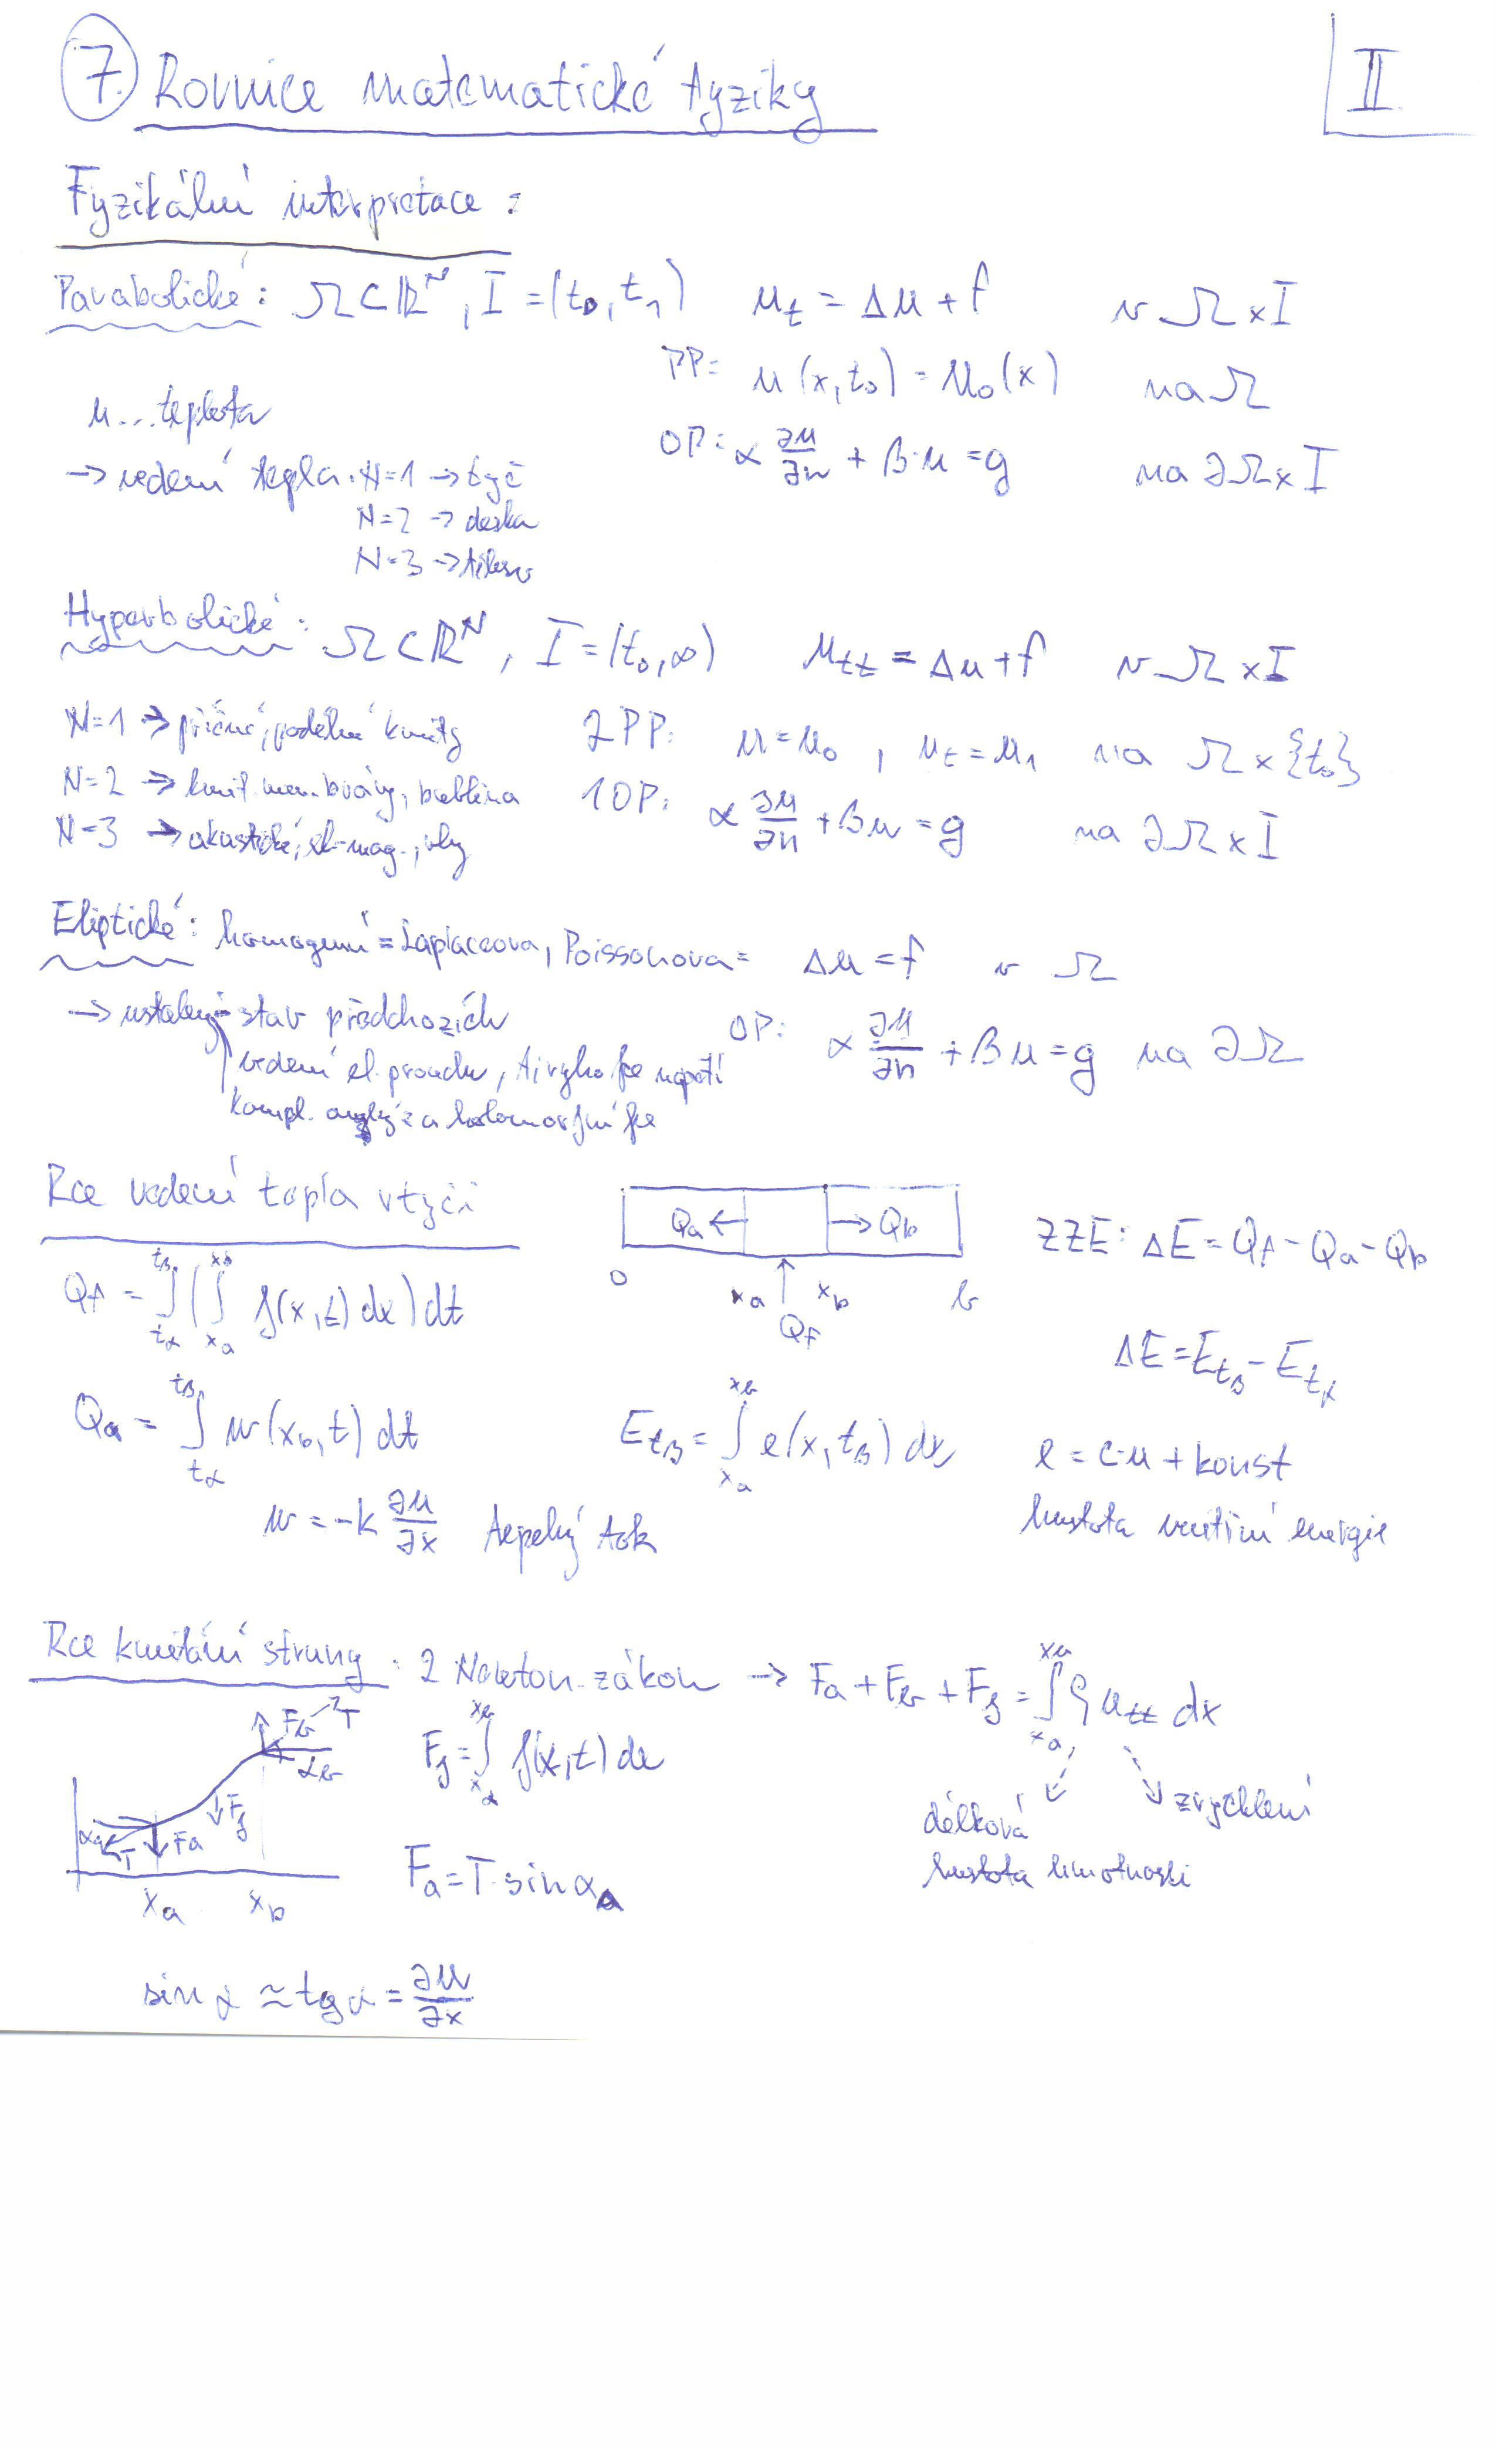
\includegraphics[width=\textwidth]{2-7a.jpg}
%\end{figure}
%\begin{figure}[h!]
%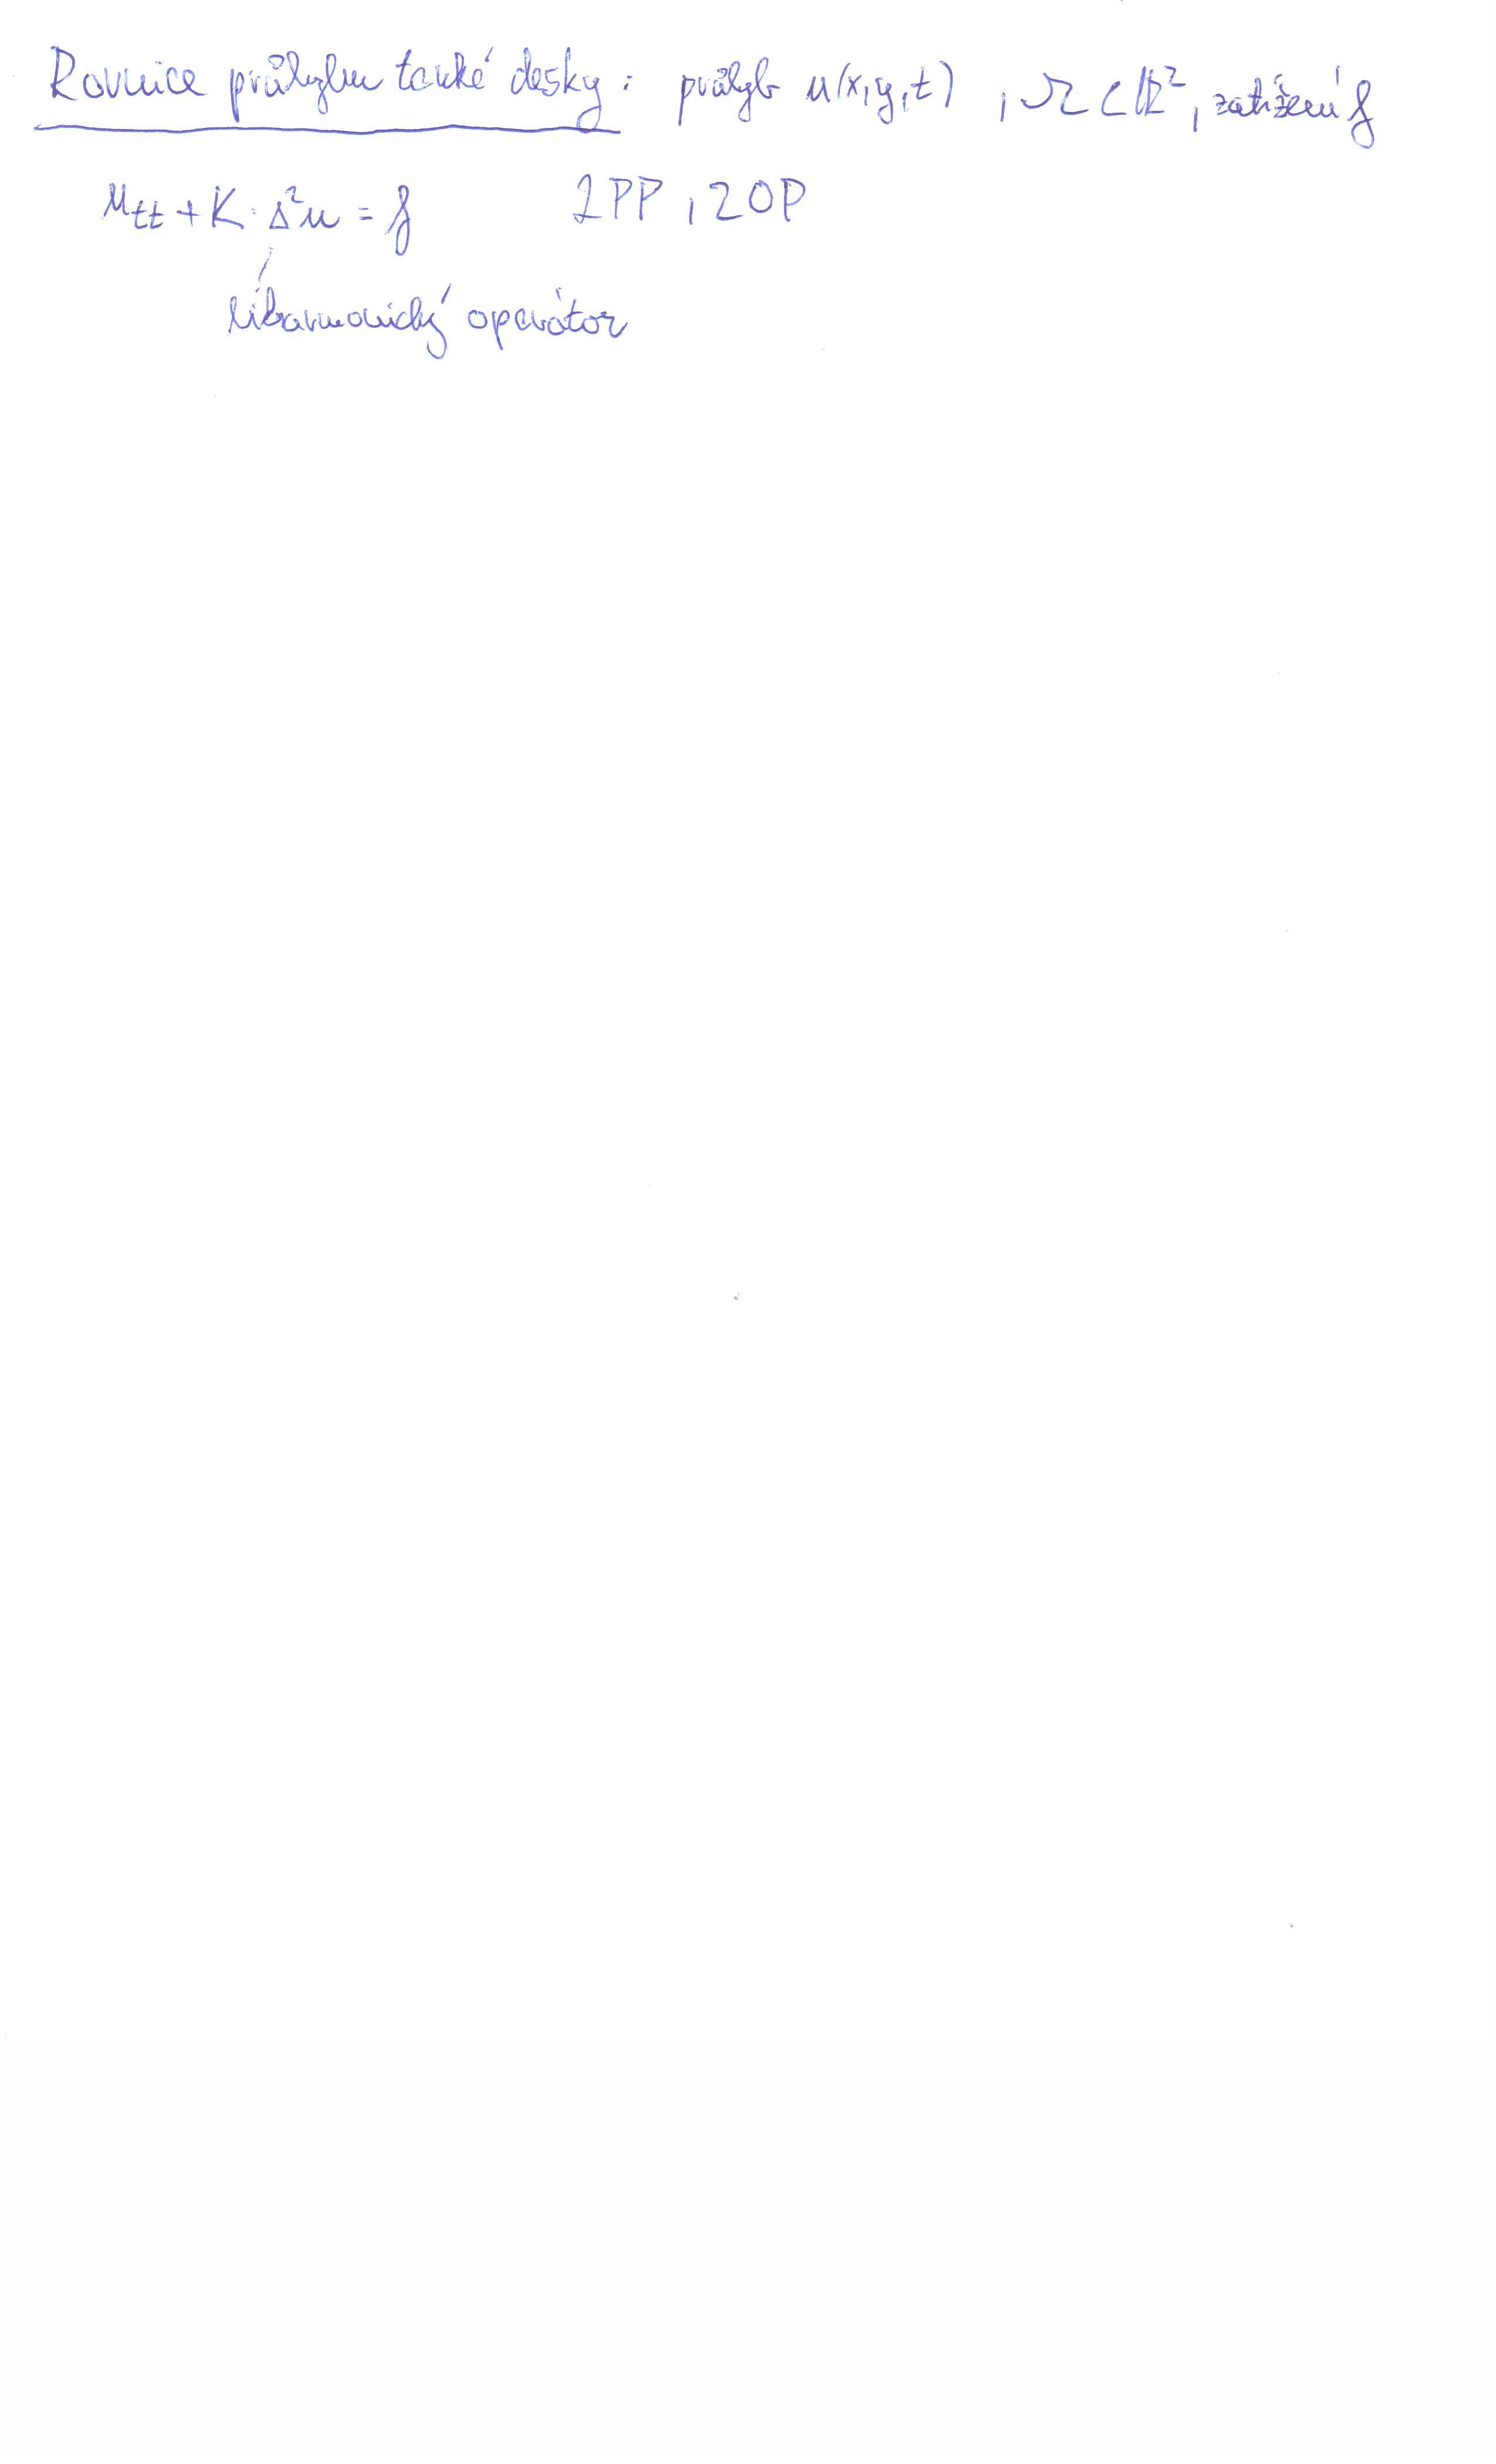
\includegraphics[width=\textwidth]{2-7b.jpg}
%\end{figure}



\section{Moderní řešení PDR}

\section{Konečnorozmérné aproximace PDR}

\section{Diferenciální geometrie}



\chapter{Optimalizace, Variační počet, Fuzzy množiny}

\section{Konečněrozměrná optimalizace lineárních úloh - základní pojmy}

\subsection{Formulace úloh LP}
\textbf{LP-problem}
Minimalizace/ maximalizace lineární funkce při lineárních omezeních typu rovnost/ nerovnost.
\newline $\mathbb{X}=(x_{1},...,x_{n})$... vektor řešení, označuje řešení optimálního problému
\newline $z=f(\mathbb{X})$... účelová funkce, je funkce vektoru řešení. Extrém účelové funkce hledáme za určitých omezujících podmínek, které ovlivňují velikost složek vektoru řešení.
\begin{enumerate}
\item[a)] omezující vlastní podmínky
\item[b)] podmínky nezápornosti (platí pro všechny složky vektoru řešení)
\end{enumerate}

\subsection{Matematická formulace}
Na množině nezáporných řešení soustavy lineárních rovnic 
$$ a_{11}x_{1}+a_{12}x_{2}+...+a_{1n}x_{n}=b_{1}$$
$$a_{m1}x_{1}+a_{m2}x_{2}+...+a_{mn}x_{n}=b_{m}$$
najděte extrém lineární funkce
$$z=c_{1}x_{1}+c_{2}x_{2}+...+c_{n}x_{n}$$
\textbf{Zjednodušený zápis:}
$$Ax=b$$
$$x\geq 0$$
$$min\; c^{T}x$$
Standardní tvar:
minimalizace:
$$min\; \; \sum_{j=1}^{n}c_{j}x_{j}$$
$$ s.t. \; \; \sum_{j=1}^{n}a_{ij}x_{j}\geq b_{i}$$
$$ x_{j}\geq 0 $$
maximalizace
$$max\; \; \sum_{j=1}^{n}c_{j}x_{j}$$
$$ s.t. \; \; \sum_{j=1}^{n}a_{ij}x_{j}\leq b_{i}$$
$$ x_{j}\geq 0 $$

\subsection{Základní pojmy}

\textbf{Konvexní množina}
$X\subset \mathbb{R}^{n}$ je konvexní množina, pokud pro $\forall x_{1},x_{2}\in X$ platí
$$\lambda \, x_{1}+(1-\lambda )\, x_{2}\in X\; \; \; \; \; \forall \lambda \in \left \langle 0,1 \right \rangle$$
Geometricky: množina X spolu s libovolnými 2 různými body musí obsahovat i úsečku, která tyto 2 body spojuje

\textbf{Polyedrická množina}
Polyedrické množiny a kužel reprezentují speciální případ konvexních množin a kuželů.
Polyedrická množina - průnik konečného počtu uzavřených poloprostorů 
$$\left \{ y: Ax\leq b \right \}$$
A...$m\, \texttt{x}\, n$ matice, b... vektor m proměnných
\newline Je možné reprezentovat pomocí konečného počtu lineárních rovnice anebo nerovnic
$$\exists k\in \mathbb{N},\; \exists \alpha _{i }\; ,\; \exists p_{i}\in \mathbb{R}^{n}\; ,\; p_{i}\neq 0$$
$$S=\bigcap_{i=1}^{k}\; \left \{ x\; |\; p_{i}^{T}x\leq \alpha _{i} \right \}$$

\textbf{Konvexní kombinace}
$x_{1},...,x_{n}\; \in \mathbb{R}^{n}\; \; \; a\; \; \; t_{1},...t_{n}$ jsou reálná čísla taková, že
\begin{enumerate}
\item[a)] $t_{i}\geq 0\; \; pro\; \; i=1,...,n$
\item[b)] $t_{1}+...+t_{n}=1$
\end{enumerate}
Potom vektor $ y=t_{1}x_{1}+...+t_{n}x_{n}$ se nazývá konvexní kombinací vektoru $x_{1},...,x_{n}$
Pokud $t_{i}\in \mathbb{R}$... afinní kombinace 
\newline Pokud $t_{i}\in \mathbb{R}\; \; a\; \; t_{1}+...+t_{n}\neq 1$... lineární kombinace

\textbf{Vlastnosti konvexních množin}

$S_{1},S_{2}\in \mathbb{R}^{n} $ konvexní $\rightarrow $ $S_{1}\cap S_{2}$, $S_{1}\oplus S_{2}$,$S_{1}\ominus S_{2}$ jsou také konvexní 

\textbf{Konvexní obal}
$S\in \mathbb{R}^{n},x\in \mathbb{R}^{n}$ patří do konvexního obalu $S\Leftrightarrow \exists k\in \mathbb{N},\; \exists \lambda _{1},...,\lambda _{n}\geq 0,\; \sum_{1}^{k}\lambda _{j}=1,\; \; \; \; \exists x_{1},...,x_{k}\in S:\; x=\sum_{j=1}^{k}\lambda _{j}x_{j}$ 
\newline příklad: Konvexní obal kružnice je kruh, pokud je množina S konvexní, potom je rovná (svému) konvexnímu obalu S.
\newline Konvexní obal je průnikem všech konvexních množin obsahujících S

\textbf{Nadrovina}

$\alpha \in \mathbb{R},\; p\in \mathbb{R}^{n},\; p\neq 0$. Nadrovina v $\mathbb{R}^{n} $: $H=\left \{ x\in \mathbb{R}^{n}|\; p^{T}x=\alpha  \right \} $
\newline -definuje 2 (otevřené/uzavřené) poloprostory:
$$H^{+}=\left \{ x\in \mathbb{R}^{n}|\; p^{T}x> (\geq )\alpha  \right \}$$
$$H^{-}=\left \{ x\in \mathbb{R}^{n}|\; p^{T}x< (\leq )\alpha  \right \}$$

\textbf{Oddělující nadrovina}
$S_{1},S_{2}\in \mathbb{R}^{n}\neq \o ,\; \; \; H=\left \{ x\; |\; p^{T}x=\alpha  \right \}$
\newline $H$ odděluje $S_{1}$ a $S_{2}\Leftrightarrow \exists i\in \left \{ 1,2 \right \}:(\forall x\in S_{i}:p^{T}x\geq \alpha )\wedge (\forall x\in S_{3-i}:p^{T}x\leq \alpha ) $  
\newline Pokud navíc $S_{1} \cup S_{2} = H\Rightarrow $ odděluje řádně.
\newline H striktně odděluje $S_{1}, S_{2}\Leftrightarrow \exists i\in \left \{ 1,2 \right \}:(\forall x\in S_{i}:p^{T}x>  \alpha )\wedge (\forall x\in S_{3-i}:p^{T}x<  \alpha )$
\newline H silně odděluje $S_{1}, S_{2}\Leftrightarrow \exists i\in \left \{ 1,2 \right \}; \exists \epsilon > 0 :(\forall x\in S_{i}:p^{T}x\geq   \alpha +\epsilon )\wedge (\forall x\in S_{3-i}:p^{T}x\leq   \alpha )$
Pozn.: $S\subset \mathbb{R}^{n} $ uzavřená + konvexní $ \Rightarrow S$ je průnik poloprostorů obsahující S



\textbf{Opěrná nadrovina}

$$ S\subset \mathbb{R}^{n}\neq \varnothing \; ,\; \bar{x} \in \partial S,\; \; \; H=\left \{ x\; |\; p^{T}(x-\bar{x})=0 \right \} $$ 
je opěrná nadrovina
$$ S\; \; v\; \; \bar{x} \Leftrightarrow S\subset H^{+}\; \vee \; S\subset H^{-}$$


\textbf{Kužel}

$C\subset \mathbb{R}^{n}$ je kužel s vrcholem 0, pokud $x \in C \Rightarrow \forall \lambda \geq 0: \; \lambda x \in C$ 
\newline S vektorem leží v lineární kombinaci.

\textbf{Polární kužel}
$ S\subset \mathbb{R}^{n}\neq \O $, potom polární kužel S označíme $polS$ nebo $S^{*}$, a $polS=\left \{  p\; |\; \forall x\in S_{i}:p^{T}x\leq  0 \right \}$




\textbf{Extrémní bod}
$ S\subset \mathbb{R}^{n}; S\neq \O $ konvexní, $x\in S$ je krajní bod $S\Leftrightarrow \forall x_{1},x_{2}\in S:\forall \lambda \in (0,1): x=\lambda x_{1}+(1-\lambda )x_{2}\Rightarrow x=x_{1}=x_{2}$
\newline Krajní bod není možné vyjádřit jako konvexní kombinaci 2 různých bodu 

\textbf{Směr}
$ S\subset \mathbb{R}^{n}\neq \O $ uzavřená, konvexní 
\newline $d\in \mathbb{R}^{n}, d\neq \o $ je směr $s\Leftrightarrow \forall x\in S, \forall \lambda \geq 0: x+\lambda d\in S$
\newline Pokud přičítám nezáporný násobek směru k jakémukoliv x, zůstanu v této množině


\textbf{Krajní směr}
Směr $d$ množiny $S$ je krajní $\Leftrightarrow (\forall d_{1},d_{2} $ směry $S$,$ \forall \lambda _{1},\lambda _{2}> 0:d=\lambda _{1}d_{1}+\lambda_{2}d_{2}\Rightarrow \exists \alpha > 0:d_{1}=\alpha d_{2})$
\newline Není možné vyjádřit jakou kladnou lineární kombinaci dvou různých směrů dané množiny


+ příklad na Krajní body a Krajní směry 

\section{Konečnorozměrná optimalizace lineárních úloh - metody řešení}
reprezentace mnoziny pripustnych reseni, podminky optimality, simplexova metoda

\section{Konečnorozměrná optimalizace nelin. úloh - základní pojmy}
\textbf{Definition}: A set $C \in E^{n}$ is said to be \textit{convex} if $\forall x_{1},x_{2} \in C$ and $\forall \alpha \in \mathbf{R}, 0 < \alpha  < 1$, the point $\alpha x_{1} + (1 - \alpha) x_{2} \in C$.

\textbf{Note: Geometrical expression of convex sets} \\
A set is convex if, given two points in the set, every point on the line segment joining these two
points is also a member of the set.

\textbf{Proposition}: Convex sets in $E^{n}$ satisfy the following relations:
\begin{enumerate}
\item If C is a convex set and $\beta$ is a real number, the set
 $\beta C = \{ \textbf{x}: \textbf{x} = \beta \textbf{c}, \textbf{c} \in C\}$
is convex.
\item If C and D are convex sets, then the set
$ C + D = \{ \textbf{x}: \textbf{x} = \textbf{c} + \textbf{d}, \textbf{c} \in C\, \textbf{d} \in D\}$
is convex.
\item The intersection of any collection of convex sets is convex.
\end{enumerate}

\textbf{Theorem: (Equivalence of extreme points and basic solutions)}. Let \textbf{A} be an
$m\times n$ matrix of rank m and \textbf{b} an m-vector. Let \textbf{K} be the convex polytope
consisting of all n-vectors x satisfying

\begin{align*}
\textbf{Ax} = \textbf{b} \\
\textbf{x} \geq \textbf{0}
\end{align*}

A vector \textbf{x} is an extreme point of \textbf{K} if and only if \textbf{x} is a basic feasible solution
to (1).

\textbf{Corollary}:
\begin{itemize}
\item If the convex set \textbf{K} corresponding to (1) is nonempty, it has at
least one extreme point.
\item If there is a finite optimal solution to a linear programming
problem, there is a finite optimal solution which is an extreme point of the
constraint set.
\item The constraint set \textbf{K} corresponding to (1) possesses at most a
finite number of extreme points.
\item If the convex polytope \textbf{K} corresponding to (1) is bounded, then \textbf{K}
is a convex polyhedron, that is, \textbf{K} consists of points that are convex
combinations of a finite number of points.
\end{itemize}




\subsection{formulace úloh NLP}

The \textit{mathematical program} (MP) is formulated as:

\begin{align*}
min \quad&  g_{0}(x) \\
s.t.\quad &  g_{i}(x) \geq 0, i=1,...,m\\
&  x \in X \subset \mathbf{R}^{n}
\end{align*}

where the set X and the functions $g_{i}: \mathbf{R}^n \rightarrow \mathbf{R}, i=1,...,m$ are given by modeling process. Depending on the properties of the problem defining functions $g_{i}$ and the
set X, MP is called
\begin{itemize}
\item \textit{linear}, if the set X is convex polyhedral and the functions $g_{i}, i = 0,...,m$
are linear
\item \textit{nonlinear}, if at least one of the functions $g_{i}, i = 0,...,m$ is nonlinear or
X is not a convex polyhedral set; among nonlinear programs, we denote
a program as
\begin{itemize}
\item \textit{convex}, if $X \cap \{x: g_{i}(x) \geq  0; i = 1, ..., m\}$ g is a convex set and $g_{0}$ is
a convex function (in particular if the functions $g_{i}; i = 0, ..., m$ are
convex and X is a convex set); and
\item \textit{nonconvex}, if either $X \cap \{x: g_{i}(x) \geq  0; i = 1, ..., m\}$ g is not a convex
set or the objective function $g_{0}$ is not convex.
\end{itemize}
\end{itemize}

\textbf{lemma}: If MP is a convex program then any local (i.e. relative)
minimum is a global minimum.

\section{Konečnorozměrná optimalizace lin. úloh - metody řešení}

\subsection{Karush-Kuhn-Tuckerovy podmínky existence extrémů a jejich geometrická interpretace}

KKT optimality conditions were independently derived by Karush in 1939 and by Kuhn{Tucker in 1951.
\newline
KKT conditions are the extension of FJ conditions (Fritz John Conditions for Inequality Constraints) with positive
Lagrange multiplier $u_{0}$ corresponding to the term $\nabla f$. In following, we can suppose that
$u_{0} = 1$ without loss of generality, since other Lagrange multipliers $u_{i}$ are just rescaled.
\bigskip

\textbf{Theorem (Karush-Kuhn-Tucker Necessary Optimality Conditions)}. \newline
Consider the problem: 

\begin{align*}
\mbox{min } \quad  f(x)\\
\mbox{s.t. } \quad g_{i}(x) \leq 0, \quad i = 1, ..., m,\\
x \in X,
\end{align*}

where $X$ is a nonempty open set in $\mathbf{E}^{N}$. Hence the feasible set $S$ is specified by 
$$S = \{x \in X, g_{i}(x) \leq 0, \forall i = 1, ..., m,\} $$

Let $X$ be a nonempty open set in $\mathbf{E}^{N}$, $f$ and $g_{i}$ $\forall i = 1, ..., m$ be
functions $f$, $g_{i}: \mathbf{E}^{N} \rightarrow \mathbf{E}$, the set $I$ be defined by 
\begin{align*}
I = \{i \in \{1,...,m\}:g_i(\overline{x})=0\}
\end{align*}
and $\overline{x}$ be a feasible point. Assume
that the functions $f$ and $g_{i}$ for all $i \in I$ are differentiable at point $\overline{x}$, the functions $g_{i}$ for
all $i \notin I$ are continuous at the point $\overline{x}$ and the gradients $\nabla g_{i}(\overline{x})$ for all $i \in I$ are linearly independent. If the point $\overline{x}$ is a local minimum to the problem (3), then there exist
numbers $u_{i}$ for all $i \in I$ such that

\begin{align*}
\nabla f(\overline{x}) + \sum_{i \in I} u_{i} \nabla g_{i}(\overline{x}) = 0, \\
u_{i} \geq 0 \quad \forall i \in I.
\end{align*}

If $g_{i}$ for all $i \notin I$ are also differentiable at point $\overline{x}$, then (5) can be rewritten to the
equivalent form

\begin{align*}
\nabla f(\overline{x}) + \sum_{i = 1}^{m} u_{i} \nabla g_{i}(\overline{x}) = 0, \\
u_{i}g_{i}(\overline{x}) = 0 \quad \forall i=1,...,m,\\
u_{i} \geq 0 \quad \forall i=1,...,m.
\end{align*}

The scalars $u_{i}$ are called the \textit{Lagrange multipliers}, as in the FJ conditions. Similarly,
the condition of feasibility of $\overline{x}$ is called the \textit{primal feasibility condition}, the conditions
$\nabla f(\overline{x}) + \sum_{i=1}^{m} u_{i} \nabla g_{i}(\overline{x}) = 0$ with $u_{i} \geq 0$ for all $i = 1,...,m$ are called the \textit{dual feasibility conditions} and the requirement $u_{i}g_{i}(\overline{x}) = 0$ for all $i = 1,...,m$ is called the 
\textit{complementary slackness condition}. The primal feasibility, dual feasibility and complementary
slackness conditions together are called the Karush-Kuhn-Tucker optimality conditions.
A point $\overline{x}$ is said to be a \textit{Karush-Kuhn-Tucker (KKT) point} if there exist Lagrange
multipliers $\overline{u}_{1}, ..., \overline{u}_{m}$ such that the point $\overline{x}$ with $\overline{u}_{1}, ..., \overline{u}_{m}$ satisfies the Karush-Kuhn-Tucker optimality conditions.
\bigskip

\textbf{Theorem (Karush-Kuhn-Tucker Suffcient Optimality Conditions)}. 
Consider the problem (3). Let $X \subset \mathbf{E}^{N}$ be a nonempty open set, $f$ and $g_{i}$ for all $i = 1,...,m$ be
functions $f, g_{i}: \mathbf{E}^{N} \rightarrow \mathbf{E}$, the set $I$ be defined by (4) and a point $\overline{x}$ be a KKT point.
Define the set $S$ by
$$S = \{ x \in X: g_{i}(x) \leq 0, i \in I \} $$
If there exists an $\varepsilon $-neighborhood $N_{\varepsilon}(\overline{x}), \varepsilon > 0$ such that $f$ is pseudoconvex over $N_{\varepsilon}(\overline{x}) \cap S$
and $g_{i}$ for $i \in I$ are differentiable at $\overline{x}$ and are quasiconvex$^{1}$ over $N_{\varepsilon}(\overline{x}) \cap S$, 
then the point $\overline{x}$ is a local minimum to the problem (3).

\textbf{footnote$^{1}$}: A function $f: S \subset \mathbf{E}^{N} \mapsto \mathbf{E}$ is said to be \textit{quasiconvex}, if for all 
$x_{1}, x_{2} \in S$ it holds
$$ f(\lambda x_{1} + (1-\lambda )x_{2}) \leq max\{ f(x_{1}),f(x_{2})\} \quad  \forall \lambda \in (0,1) $$

\textbf{Note}: Note that the set $S$ is, as in Fritz John Suffcient Optimality Conditions, the relaxation of the feasible region of (3)
since all non-active constraints $g_{i}$ are taken out. Also note that it can be shown that if $f$
and $g_{i}$ are convex at the point $\overline{x}$, then KKT conditions (6) are suffcient.

\subsection{Základní numerické algoritmy}


\section{Řešení úloh variačního počtu}

\subsection{Minimalizace funkcionálu}
Jde o minimalizaci funkcionálu, který je ve formě integrálu $J=\int_{a}^{b}L(x,y,{y}')dx $. Chceme zjistit, pro jaké $y$ nabývá $J$ minimální hodnoty. 
Řekneme, že funkce $y$ realizuje minimum funkcionálu $J$, pokud pro $\forall y+\epsilon \eta  $, kde $\epsilon $ je reálné kladné nebo záporné číslo (ne 0).
\newline $\eta (x)$ je funkce taková, že $\eta (a)=\eta (b)=0\; \; \; \; ,\eta \not\equiv 0$
\newline $J:C^{1}\left \langle a,b \right \rangle\rightarrow \mathbb{R}$ hladká spojitá funkce s 1. derivací
\newline Platí $J(y+\epsilon \eta )-J(y)> 0$
\newline Dále $J(y+\epsilon \eta )-J(y)=\int_{a}^{b}L(x,y+\epsilon \eta ,{y}'+\epsilon {\eta }')dx-\int_{a}^{b}L(x,y,{y}')dx=...Taylor\; \;  rozvoj...=\epsilon J_{1}+\frac{1}{2}\epsilon ^{2}J_{2}+O(\epsilon ^{3})$
\newline Nutná podmínka extrému: $J_{1}=0$... vyšetření 1. variace
\newline Postačující podmínka minima: $J_{1}=0,\; J_{2}> 0$... vyšetření 2. variace

\subsection{Základní lemma variačního počtu}

Je dána spojitá funkce na $\left \langle a,b \right \rangle$ ozn. $\Phi (x)$. Pokud pro každou funkci $\eta (x)$ spojitou na $\left \langle a,b \right \rangle$ platí $\int_{a}^{b}\Phi (x)\eta (x)dx=0$, potom $\Phi (x)=0$.
 Důkaz sporem.

\subsection{Eulerova rovnice}
$$J_{1}=0,\; \; J_{1}=\int_{a}^{b}(\eta\frac{\partial L}{\partial y} +{\eta }'\frac{\partial L}{\partial {y}'})dx$$
$$J_{1}=\int_{a}^{b}(\eta\frac{\partial L}{\partial y} +{\eta }'\frac{\partial L}{\partial {y}'})dx=0...per\; \; partes...\Rightarrow \int_{a}^{b}\eta (\frac{\partial L}{\partial y}-\frac{\mathrm{d} }{\mathrm{d} x}\frac{\partial L}{\partial {y}'})dx=0$$
má být splněno pro $\forall \eta $, proto podle základního lemmatu můžeme psát:
$$\frac{\partial L}{\partial y}-\frac{\mathrm{d} }{\mathrm{d} x}\frac{\partial L}{\partial {y}'}=0$$
řešení tohoto problému jsou stacionární křivky


\subsection{Druhá variace}

$$J_{2}=\int_{a}^{b}(\eta ^{2}P+2\eta {\eta }'Q+{\eta }'^{2}R)dx$$
, kde $P=\frac{\partial^2 L}{\partial y^2} $, $Q=\frac{\partial^2 L}{\partial y\partial {y}'} $, $R=\frac{\partial^2 L}{\partial {y}'^2} $. 
\newline $J_{2}> 0$ pro minimum 
\newline $J_{2}< 0$ pro maximum
\newline Použitím množství technických lemmat ukážeme, že znaménko u $R=\frac{\partial^2 L}{\partial {y}'^2} $ je pro znaménko $J_{2}$ rozhodující.
Na to, aby se dokázalo, že $y$ realizuje minimum (resp. maximum) se používá Legendrov test: 
  \begin{enumerate}
\item[1)] pro funkci $y$ je splněna Eulerova rovnice
\item[2)] $\left \langle a,b \right \rangle$ je dostatečně malý interval
\item[3)] $\frac{\partial^2 L}{\partial {y}'^2}>0$ nemění znaménko na $(a,b)$

\end{enumerate}
Pozn.: Pokud jsou a, b dostatečně blízko $\rightarrow$ Konjugované body

\subsection{Konjugované body}

První konjugovaný bod $A^{*}$ k bodu $A$.
\newline 2 možnosti:
  \begin{enumerate}
\item[-] $A^{*}$ je před $B \rightarrow$ extrém nenastává
\item[-] $A^{*}$ je za $B \rightarrow$ extrém může nastat \begin{enumerate}
\item[a)] $R$ nemění znaménko na $\left \langle a,b \right \rangle \rightarrow$ jde o extrém
\item[b)] $R$ mění znaménko na $\left \langle a,b \right \rangle \rightarrow$ není to extrém 
\end{enumerate}

\end{enumerate}

Analytický způsob hledání konjugovaných bodů:
$$ \frac{\frac{\partial y}{\partial c_{1}}(a)}{\frac{\partial y}{\partial c_{2}}(a)}=\frac{\frac{\partial y}{\partial c_{1}}(x)}{\frac{\partial y}{\partial c_{2}}(x)}$$
$y$- obecné řešení, $a$- z okrajových podmínek. Řešením je $x\neq a$

\subsection{Aplikace}
\begin{enumerate}
\item[-]Minimální plochy - rotace křivky kolem osy x. Zobecnění - napínání plochy na křivku tak, aby byl obsah minimální
\item[-]Geodetiky - křivky na ploše, spojuji body tak, aby délka křivky na ploše byla minimální
\item[-]Balistická křivka
\item[-]Řetězovka
\item[-]Gaussova funkce
\end{enumerate}

\section{Optimální řízení dynamických systémú}

\textit{Přípustné a optimální regulace, základní úloha optimálního řízení, princip maxima, podmínky transverzality, aplikace}\\

\begin{definition}
Vektorový prostor $X$ je \textit{stavový (fázový) prostor} proměnných $x(t)=(x_1(t),...x_n(t))$, který popisuje pohyb objektu v čase. Předpokladáme regulovatelnost pohybu.
\end{definition}
\begin{definition}
Vektorová proměnná $u(t)=(u_1(t),...u_n(t))$ definována na nejakém intervalu $[t_0,t_1]$ se nazývá \textit{regulace}. Její obor hodnot $U$ se nazývá \textit{obor regulace}. $U$ je uzavřená podmnožina Euklidovského prostoru.
\end{definition}

\section{ Fuzzy množiny}
základní pojmy, inkluze a operace, t-normy a t-konormy, silná negace, alfa řezy, princip rozšíření, reálná fuzzy čísla a operace

\subsection{Základní pojmy, inkluze a operace, alfa řezy}

\begin{definition}
Nechť $X \neq \emptyset$ je množina a $\muA: X \rightarrow \langle 0;1 \rangle$ je zobrazení. \textbf{Fuzzy množinou} $\fA$ na $X$ rozumíme množinu všech uspořádaných dvojic $\lbrace (x, \muA(x)); x \in X, \muA(x) \in \langle 0;1 \rangle \rbrace$ a píšeme $\fA = (X; \muA)$. Množina $X$ je \textbf{univerzum}, zobrazení $\muA$ je \textbf{funkce příslušnosti} fuzzy množiny $\fA$ a $\muA(x)$ je \textbf{stupeň příslušnosti} prvku $x$ k $\fA$ pro $\forall x \in X$.
\end{definition}

\begin{remark}
Zobrazení $\muA$ je definováno pro $\forall x \in X$. Pro $x \notin \fA$ klademe $\muA(x)=0$.
\end{remark}

\begin{definition}
\textbf{Nosičem (základem)} fuzzy množiny $\fA$ rozumíme množinu supp $\fA = \lbrace x \in X; \muA(x) > 0 \rbrace$.
\end{definition}

\begin{definition}
\textbf{Jádrem} fuzzy množiny $\fA$ rozumíme množinu ker $\fA = \lbrace x \in X; \muA(x) = 1 \rbrace$.
\end{definition}

\begin{definition}
\textbf{Výškou} fuzzy množiny $\fA$ rozumíme množinu hgt $\fA = \sup\limits_{x \in X} \muA(x)$.
\end{definition}

\begin{definition}
Fuzzy množina $\fA$ je \textbf{normální}, jestliže $\exists x \in X$ takové, že $\muA(x) = 1$.
\end{definition}

\begin{definition}
Fuzzy množina $\fA$ je \textbf{podmnožinou} fuzzy množiny $\fB$ a píšeme $\fA \subset \fB$, jestliže $\muA(x) \leq \muB(x)$ pro $\forall x \in X$.
\end{definition}

\begin{definition}
Fuzzy množiny $\fA$ a $\fB$ jsou si \textbf{rovny} a píšeme $\fA = \fB$, jestliže $\muA(x) = \muB(x)$ pro $\forall x \in X$.
\end{definition}

\begin{definition}
\textbf{Průnik} fuzzy množin $\fA$ a $\fB$ je fuzzy množina $\fA \cap \fB$, kde
\begin{equation*}
\mu_{\fA \cap \fB}(x) = \min \lbrace \muA(x), \muB(x) \rbrace \text{ pro } \forall x \in X.
\end{equation*}
\end{definition}

\begin{definition}
\textbf{Sjednocení} fuzzy množin $\fA$ a $\fB$ je fuzzy množina $\fA \cup \fB$, kde
\begin{equation*}
\mu_{\fA \cup \fB}(x) = \max \lbrace \muA(x), \muB(x) \rbrace \text{ pro } \forall x \in X.
\end{equation*}
\end{definition}

\begin{definition}
\textbf{Doplňkem} fuzzy množiny $\fA$ rozumíme fuzzy množinu $\overline{\fA}$, kde
\begin{equation*}
\mu_{\overline{\fA}}(x) = 1 - \muA(x) \text{ pro } \forall x \in X.
\end{equation*}
\end{definition}

\begin{theorem}
Pro libovolné fuzzy množiny $\fA, \fB, \fC$ platí
\begin{table}[H]
\centering
\begin{tabular}{ll}
$\fA \cap \fB = \fB \cap \fA$                                 & $\fA \cap \emptyset = \emptyset$                             \\
$\fA \cup \fB = \fB \cup \fA$                                 & $\fA \cup \emptyset = \fA$                                   \\
$\fA \cap (\fB \cap \fC) = (\fA \cap \fB) \cap \fC$           & $\fA \cap X = \fA$                                           \\
$\fA \cup (\fB \cup \fC) = (\fA \cup \fB) \cup \fC$           & $\fA \cup X= X$                                              \\
$\fA \cap \fA = \fA$                                          & $\overline{(\overline{\fA})} = \fA$                          \\
$\fA \cup \fA = \fA$                                          & $\overline{\fA \cap \fB}=\overline{\fA} \cup \overline{\fB}$ \\
$\fA \cap (\fB \cup \fC)= (\fA \cap \fB) \cup (\fA \cap \fC)$ & $\overline{\fA \cup \fB}=\overline{\fA} \cap \overline{\fB}$ \\
$\fA \cup (\fB \cap \fC)= (\fA \cup \fB) \cap (\fA \cup \fC)$ &                                                             
\end{tabular}
\end{table}
\end{theorem}


\begin{remark}
Operace $\cup, \cap$ rozšiřujeme pro libovolnou indexovou množinu $I$ pomocí vztahů
\begin{equation*}
\mu_{\bigcap\limits_{i \in I} \underset{^\sim}{A_i}}(x) = \inf_{\substack{i \in I}} \mu_{\underset{^\sim}{A_i}}(x), \qquad \mu_{\bigcup\limits_{i \in I} \underset{^\sim}{A_i}}(x) = \sup_{\substack{i \in I}} \mu_{\underset{^\sim}{A_i}}(x) \quad \text{ pro } \forall x \in X.
\end{equation*}
\end{remark}

\begin{definition}
\textbf{Součinem} fuzzy množin $\fA$ a $\fB$ rozumíme fuzzy množinu $\fA \cdot \fB$, kde
\begin{equation*}
\mu_{\fA \cdot \fB}(x) =  \muA(x) \cdot \muB(x) \text{ pro } \forall x \in X.
\end{equation*}
\end{definition}

\begin{definition}
\textbf{Součtem} fuzzy množin $\fA$ a $\fB$ rozumíme fuzzy množinu $\fA + \fB$, kde
\begin{equation*}
\mu_{\fA + \fB}(x) =  \muA(x) + \muB(x) - \muA(x) \cdot \muB(x) \text{ pro } \forall x \in X.
\end{equation*}
\end{definition}

\begin{theorem}
Pro libovolné fuzzy množiny $\fA, \fB, \fC$ platí
\begin{table}[H]
\centering
\begin{tabular}{ll}
$\fA \cdot \fB = \fB \cdot \fA$                         & $\fA + \emptyset = \fA$                                    \\
$\fA + \fB = \fB + \fA$                                 & $\fA \cdot X= \fA$                                           \\
$\fA \cdot (\fB \cdot \fC) = (\fA \cdot \fB) \cdot \fC$ & $\fA + X = X$                                              \\
$\fA + (\fB + \fC) = (\fA + \fB) + \fC$                 & $\overline{\fA \cdot \fB}=\overline{\fA} + \overline{\fB}$ \\
$\fA \cdot \emptyset = \emptyset$                       & $\overline{\fA + \fB}=\overline{\fA} \cdot \overline{\fB}$
\end{tabular}
\end{table}
\end{theorem}

\begin{remark}
Neplatí distributivita operací $\cdot, +$ ani idempotence. Operace $\cdot, +$ jsou distributivní vzhledem k $\cup, \cap$, nikoli naopak. Obecně platí
\begin{equation*}
\fA \cdot \fB \subset \fA \cap \fB \subset \fA \cup \fB \subset \fA + \fB.
\end{equation*}
\end{remark}

\begin{definition}
Nechť $m \in (0, \infty)$. \textbf{m-tou mocninou} fuzzy množiny $\fA$ rozumíme fuzzy množinu $\fA^m$, kde $\mu_{\fA^m}(x)=[\muA(x)]^m$ pro $\forall x \in X$.
\end{definition}

\begin{definition}
Nechť $\alpha \in \langle 0, 1 \rangle$. {\boldmath$\alpha$}\textbf{-násobkem} fuzzy množiny $\fA$ rozumíme fuzzy množinu $\alpha\fA$, kde $\mu_{\alpha\fA}(x)=\alpha\muA(x)$ pro $\forall x \in X$.
\end{definition}

\begin{definition}
Nechť $\alpha \in \langle 0, 1 \rangle$. {\boldmath$\alpha$}\textbf{-řezem} fuzzy množiny $\fA$ rozumíme obyčejnou množinu
\begin{equation*}
A_{\alpha} = \lbrace x \in X; \muA(x) \geq \alpha \rbrace.
\end{equation*}
\end{definition}

\begin{theorem}
Pro libovolné fuzzy množiny $\fA$ platí
\begin{eqnarray*}
\muA(x) &=& \sup_{\substack{\alpha \in (0;1\rangle}} \min \big(\alpha, \mu_{A_{\alpha}}(x)\big) \quad \text{ pro } \forall x \in X, \\
\fA &=& \bigcup\limits_{\alpha \in \langle 0;1 \rangle} \alpha A_{\alpha}, \\
\alpha_1 \leq \alpha_2 &\Rightarrow& A_{\alpha_2} \subset A_{\alpha_1}.
\end{eqnarray*}
\end{theorem}

\begin{definition}
Fuzzy množina $\fA$ je \textbf{konvexní}, jestliže jsou konvexní všechny její $\alpha$-řezy.
\end{definition}

\subsection{T-norma (trojúhelníková norma)}

\begin{definition}
Zobrazení $t:\langle 0,1\rangle \times \langle 0,1\rangle \rightarrow \langle 0,1\rangle$ se nazývá t-norma, splňuje-li následující podmínky:

\begin{itemize}
\item  t je neklesající v obou argumentech
\item  $t(x,y)=t(y,x)$  $\forall x,y\in \langle 0,1 \rangle$ (komutativita)
\item  $t(x,t(y,z))=t(t(x,y),z) $  $\forall x,y,z\in \langle 0,1 \rangle$ (asociativita)
\item $t(1,x)=x$  $\forall x\in \langle 0,1 \rangle$ (hraniční podmínka)
\end{itemize}
\end{definition}

Základní t-normy:
\begin{itemize}
\item Minimová: $T_M (x,y)=min\{x,y\}$,
\item Součinová: $T_P (x,y)=xy$,
\item Łukasiewiczova: $T_L (x,y)=max\{0,x+y-1\}$,
\item Drastický součin: $T_D(x,y)=min\{x,y\}$ pokud $max\{x,y\}=1$ jinak $T_D(x,y)=0$.
\end{itemize}



\subsection{T-konorma (trojúhelníková konorma)}

\begin{definition}
Zobrazení $s:\langle 0,1\rangle \times \langle 0,1\rangle \rightarrow \langle 0,1\rangle$ se nazývá t-konorma, splňuje-li následující podmínky:
\begin{itemize}
\item  t je neklesající v obou argumentech
\item  $s(x,y)=s(y,x)$  $\forall x,y\in \langle 0,1 \rangle$ (komutativita)
\item  $s(x,s(y,z))=s(s(x,y),z) $  $\forall x,y,z\in \langle 0,1 \rangle$ (asociativita)
\item $s(0,x)=x$  $\forall x\in \langle 0,1 \rangle$ (hraniční podmínka)
\end{itemize}
\end{definition}

Příklady t-konormy:
\begin{itemize}
\item Maximová: $S_M (x,y)=max\{x,y\}$, 
\item Pravděpodobnostní součet: $S_P(x,y)=x+y-xy$, 
\item Łukasiewiczova: $S_L (x,y)=min\{1,x+y\}$,
\item Drastický součet: $S_D(x,y)=max\{x,y\}$ pokud $min\{x,y\}=0$ jinak $S_D(x,y)=1$.
\end{itemize}






\subsection{Silná negace}
\begin{definition}
\textbf{Fuzzy negace} je libovolná funkce $n:\langle 0,1\rangle \rightarrow \langle 0,1\rangle$ s vlastnostmi:
\begin{enumerate}
\item $n(0) = 1, \quad n(1) = 0,$
\item $\forall x,y \in \langle 0,1\rangle:  x<y \Rightarrow n(x) \geq n(y)$ (nerostoucí funkce). 
\end{enumerate}
\end{definition}

\begin{definition}
Fuzzy negace $n$, která je klesající a spojitá se nazývá \textbf{striktní fuzzy negace}.
\end{definition}

\begin{definition}
Fuzzy negace $n$, která je involutivní, tj. $n(n(x))=x$ pro $\forall x \in \langle 0,1\rangle$, se nazývá \textbf{silná fuzzy negace}.
\end{definition}

\begin{remark}
Funkci $n(x)=1-x, x \in \langle 0,1\rangle$ budeme nazývat \textbf{standardní fuzzy negací}. Je zřejmé, že tato fuzzy negace je striktní i silná.  
\end{remark}

\begin{theorem}
Každá silná fuzzy negace je i striktní.
\end{theorem}



\subsection{Princip rozšíření}

\begin{definition}
Nechť $X_1 \times \ldots \times X_n$ je kartézský součin univerz $X_1, \ldots, X_n$ a $\underset{^\sim}{A_1} = (X_1, \mu_{\underset{^\sim}{A_1}}), \ldots, \underset{^\sim}{A_n} = (X_n, \mu_{\underset{^\sim}{A_n}})$ jsou fuzzy množiny. \textbf{Kartézský součin} fuzzy množin je fuzzy množina $\underset{^\sim}{A_1} \times \ldots \times \underset{^\sim}{A_n} = (X_1 \times \ldots \times X_n; \mu_{\underset{^\sim}{A_1} \times \ldots \times \underset{^\sim}{A_n}})$, kde
\begin{equation*}
\mu_{\underset{^\sim}{A_1} \times \ldots \times \underset{^\sim}{A_n}}(x_1, \ldots, x_n) = \min\lbrace \mu_{\underset{^\sim}{A_1}}(x_1), \ldots, \mu_{\underset{^\sim}{A_n}}(x_n) \rbrace \; \text{ pro } \forall(x_1, \ldots, x_n) \in X_1 \times \ldots \times X_n.
\end{equation*}
\end{definition}

\begin{definition}[\textbf{Zadehův princip rozšíření}]
Nechť $\underset{^\sim}{A_1} = (X_1, \mu_{\underset{^\sim}{A_1}}), \ldots, \underset{^\sim}{A_n} = (X_n, \mu_{\underset{^\sim}{A_n}})$ jsou fuzzy množiny a $f: X_1 \times \ldots \times X_n \rightarrow Y$ je zobrazení. Říkáme, že fuzzy množina $\fB = f(\underset{^\sim}{A_1}, \ldots, \underset{^\sim}{A_n})$ je \textbf{fuzzy hodnotou funkce f podle principu rozšíření}, jestliže
\begin{equation*}
\muB(y)=
 \begin{cases}
\sup\limits_{\substack{(x_1, \ldots, x_n) \\ f(x_1, \ldots, x_n)=y}} \min\lbrace \mu_{\underset{^\sim}{A_1}}(x_1), \ldots, \mu_{\underset{^\sim}{A_n}}(x_n) \rbrace, \\
\bigskip
\\
 0\qquad \text{ když }  f^{-1}(y) = \emptyset, 
  \end{cases}
\end{equation*}
kde $f^{-1}(y)$ je množina všech $n$-tic $(x_1, \ldots, x_n)$ takových, že $y = f(x_1, \ldots, x_n)$.
\end{definition}

\begin{remark}\label{prosty-zadeh}
Nechť $n=1$ a $f$ je prosté zobrazení. Pak pro $\fB = f(\fA)$ platí $\muB(y)=\muA(f^{-1}(y))$.
\end{remark}



\subsection{Reálná fuzzy čísla a operace}

\begin{definition}
Fuzzy množina $\fa = (\mathbb{R}, \mua)$ se nazývá \textbf{fuzzy číslo}, jestliže fuzzy množina $\fa$ je konvexní a normální a $\mua$ je po částech spojitá funkce. Jestliže existuje právě jedno $a \in \mathbb{R}$ takové, že $\mua(a)=1$, pak říkáme, že $a$ je \textbf{hlavní hodnota} fuzzy čísla $\fa$. Je-li funkce příslušnosti $\mua$ spojitá, říkáme, že $\fa$ je \textbf{spojité fuzzy číslo}. Množinu všech fuzzy čísel na $\mathbb{R}$ značíme $\mathcal{A}$. 
\end{definition}

\begin{definition}
Nechť $\varphi$ je unární operace na $\mathbb{R}$. \textbf{Rozšířenou unární operací na} $\mathcal{A}$ rozumíme (podle principu rozšíření) operaci $\varphi(\fa), \fa \in \mathcal{A}$, kde $\mu_{\varphi(\fa)}(y) = \sup\limits_{\substack{x \\ \varphi(x)=y}} \mua(x)$. Pro $\varphi$ prosté viz poznámku \ref{prosty-zadeh}.
\end{definition}

\begin{definition}
Je-li $\varphi(x)=-x$, pak $-\fa$ se nazývá \textbf{opačné fuzzy číslo} k fuzzy číslu $\fa$. Je-li $\varphi(x)=x^{-1}$, pak $\fa^{-1}$ se nazývá \textbf{inverzní fuzzy číslo} k fuzzy číslu $\fa$. Je-li $\varphi(x)=\lambda x, \lambda \in \mathbb{R}$, pak $\lambda \fa$ se nazývá {\boldmath$\lambda$}\textbf{-násobek fuzzy čísla} $\fa$. Je-li $\varphi(x)=e^{x}$, pak $e^{\fa}$ se nazývá \textbf{exponenciála fuzzy čísla} $\fa$. Říkáme, že fuzzy číslo $\fa$ je \textbf{kladné}, resp. \textbf{záporné}, jestliže $\mua(x)=0$ pro $\forall x < 0$, resp. $\forall x > 0$. Píšeme $\fa>0$, resp. $\fa < 0$.
\end{definition}

\begin{theorem}
Nechť $\fa$ je fuzzy číslo. Pak platí:
\begin{enumerate}
\item $-\fa$ je fuzzy číslo a $\mu_{-\fa}(x)=\mua(-x), \forall x \in \mathbb{R}$.
\item $\mu_{\fa^{-1}}(x) =
	\begin{cases}
		\mua(x^{-1}), \forall x \in \mathbb{R} - \lbrace 0 \rbrace, \\
		0, \qquad x=0
    \end{cases}$ \\
    a pro $\fa > 0$ nebo $\fa < 0$ je $\fa^{-1}$ fuzzy číslo.
\item $\lambda\fa$ je fuzzy číslo, přičemž pro $\lambda \neq 0$ je $\mu_{\lambda\fa}(x)=\mua(x/\lambda)$ a pro $\lambda = 0$ je $\mu_{\lambda\fa}(x) = \mu_{\lbrace 0 \rbrace}(x), \forall x \in \mathbb{R}$.
\item $e^{\fa}$ je fuzzy číslo a $\mu_{e^{\fa}}(x) = \begin{cases}
\mua(\ln{x}), x > 0, \\
0, \quad x \leq 0.
\end{cases}$
\end{enumerate}
\end{theorem}

\begin{definition}
Nechť $\ast$ je binární operace na $\mathbb{R}$. \textbf{Rozšířenou binární operací na} $\mathcal{A}$ rozumíme podle principu rozšíření operaci $\circledast$, přičemž
\begin{equation*}
\mu_{\fa \circledast \fb}(z) = \sup\limits_{\substack{x, y \\ x \ast y = z}} \min \lbrace \mua(x), \mub(y) \rbrace.
\end{equation*}
\end{definition}

\begin{definition}
Binární operace $\ast$ na $\mathbb{R}$ se nazývá \textbf{rostoucí}, resp. \textbf{klesající}, jestliže pro libovolné $x_1 > x_2$ a $y_1 > y_2$ platí $x_1 \ast y_1 > x_2 \ast y_2$, resp. $x_1 \ast y_1 < x_2 \ast y_2$.
\end{definition}

\begin{theorem}
Nechť $\ast$ je spojitá rostoucí anebo klesající binární operace na $\mathbb{R}$ a $\fa, \fb$ jsou spojitá fuzzy čísla. Pak $\fa \circledast \fb$ je spojité fuzzy číslo a $\fa \circledast \fb = \bigcup\limits_{\alpha \in \langle 0; 1 \rangle} \alpha (a_{\alpha} \ast b_{\alpha})$, kde $a_{\alpha}, b_{\alpha}$ jsou $\alpha$-řezy fuzzy čísel $\fa, \fb$.
\end{theorem}

\begin{dusledek}
Jsou-li $\fa, \fb$ spojitá fuzzy čísla a $\ast$ je spojitá binární operace na $\mathbb{R}$, pak platí
\begin{equation*}
\fa \circledast \fb =
\begin{cases}
\bigcup\limits_{\alpha \in \langle 0; 1 \rangle} \alpha \langle a_{1\alpha} \ast b_{1\alpha}; a_{2\alpha} \ast b_{2\alpha} \rangle \quad \text{pro $\ast$ rostoucí,}\\
\bigcup\limits_{\alpha \in \langle 0; 1 \rangle} \alpha \langle a_{2\alpha} \ast b_{2\alpha}; a_{1\alpha} \ast b_{1\alpha} \rangle \quad \text{pro $\ast$ klesající.}
\end{cases}
\end{equation*}
\end{dusledek}

\begin{theorem}
Nechť $\ast$ je binární operace na $\mathbb{R}$. Pak platí:
\begin{enumerate}
\item $\ast$ komutativní $\Rightarrow \circledast$ komutativní,
\item $\ast$ asociativní $\Rightarrow \circledast$ asociativní,
\item $\circledast$ je distributivní vzhledem k $\cup$.
\end{enumerate}
\end{theorem}

\begin{dusledek}
Protože $+$ je spojitá rostoucí binární operace na $\mathbb{R}$, je rozšířený součet $\oplus$ spojitých fuzzy čísel spojité fuzzy číslo. Platí $-(\fa \oplus \fb) = (-\fa) \oplus (-\fb)$. $\oplus$ je komutativní a asociativní, avšak obecně neplatí $\fa \oplus (-\fa) = 0$.
\end{dusledek}

\begin{dusledek}
Protože násobení $\cdot$ je spojitá operace, která je rostoucí na $\mathbb{R}^+$ a klesající na $\mathbb{R}^-$, je rozšířený součin $\otimes$ kladných anebo záporných spojitých fuzzy čísel spojité fuzzy číslo. Platí $-(\fa) \otimes \fb = -(\fa \otimes \fb)$. $\otimes$ je komutativní a asociativní, avšak obecně neplatí $\fa \otimes \fa^{-1} = 1$.
\end{dusledek}

\begin{theorem}
Nechť $\fa$ je kladné anebo záporné spojité fuzzy číslo, $\fb, \fc$ spojitá fuzzy čísla. Pak je $\fa \otimes (\fb \otimes \fc) \subset (\fa \otimes \fb) \oplus (\fa \otimes \fc)$. Jsou-li $\fb, \fc$ současně kladná anebo záporná spojitá fuzzy čísla, je $\fa \otimes (\fb \oplus \fc)$ spojité fuzzy číslo a platí $\fa \otimes (\fb \otimes \fc) = (\fa \otimes \fb) \oplus (\fa \otimes \fc)$.
\end{theorem}

\section{Lagrangeovský a Hamiltonovský formalizmus variačného počtu}

\section{Lineární úloha časové optimalizace}

\section{Aplikace fuzzy množin}
T-normy, konormy; unární, bin operace; fuzzy cisla; fuzzy relace; fuzzy regulace
\subsection{T-norma}
Funkce T: $\langle0,1\rangle^2\mapsto\langle0,1\rangle$ se nazývá \textbf{TROJUHELNÍKOVÁ NORMA} (t-norma), když pro každé x,y,z: 

\begin{itemize}
\item[-]{$T(x,y)=T(y,x)$}
\item[-]{$T(x,T(y,z))=T(T(x,y),z)$}
\item[-]{$T(x,y)\leq T(x,z)\quad \text{když} \quad y\leq z$}
\item[-]{$T(x,1)=x$}
\end{itemize}

\subsection{T-konorma}
Funkce S: $\langle0,1\rangle^2\mapsto\langle0,1\rangle$ se nazývá \textbf{TROJUHELNÍKOVÁ KONORMA} (t-norma), když pro každé x,y,z: 

\begin{itemize}
\item $S(x,y)=S(y,x)$
\item $S(x,S(y,z))=S(S(x,y),z)$
\item $S(x,y) \leq S(x,z)\quad \text{když} \quad y\leq z$
\item $S(x,0)=x$
\end{itemize}

\subsubsection{VĚTA}
Funkce S je t-konorma právě když 
$S(x,y)=1-T(1-x,1-y)$, kde T je t-norma.
\subsection{fuzzy relace}
Binární relaci R z množiny $\mathbb{X}$ do množiny $\mathbb{Y}$ je jakákoliv podmnožina R kartézského součinu $\mathbb{X}\times\mathbb{X}$. $R\subseteq\mathbb{X}\times\mathbb{X}$
\subsection{fuzzy čísla}
\subsubsection{aritmetické operace s fuzzy čísly pomocí $\alpha$-řezů}
Pro libovolné fuzzy množiny \textit{A} platí: $A=\bigcup\limits_{\alpha \in <0,1>} \alpha A_{\alpha}$
tento princip využijeme při počítání aritmetických operací $\alpha$-řezů. 
Nechť $\ast$ je libovolná operace +, -, /, $\cdot$. Příslušné operace s intervaly jsou definovány $$\langle a,b \rangle \circledast \langle c,d\rangle= \left \{ u\ast v\,|\, u \in \langle a,b\rangle \wedge v \in \langle c,d\rangle \right \}$$ z čehož definujeme operace:$\langle a,b \rangle \oplus \langle c,d\rangle = \langle a+c,b+d\rangle $, $\langle a,b \rangle \ominus \langle c,d\rangle = \langle a-c,b-d\rangle $, $\langle a,b \rangle \odot \langle c,d\rangle = \langle min(ac, ad, bc, bd),max(ac, ad, bc, bd)\rangle $ a $\langle a,b \rangle \oslash \langle c,d\rangle = \langle a,b \rangle \odot \langle 1/c,1/d\rangle $.
Příklad: Mějme součin fuzzy čísel A=(1,1,1) a B=(3,1,2).(Rozuměj délka ramena vlevo, support, délka ramena vpravo.)
$A^{(\alpha)}=\langle \alpha, 2-\alpha \rangle$, $B^{(\alpha)}=\langle 2 + \alpha, 5-2\alpha \rangle$. Součiny jsou tedy $s_1^{(\alpha)}=\alpha^2 +2\alpha$, $s_2^{(\alpha)}=4-\alpha^2$, $s_3^{(\alpha)}=5\alpha-2\alpha^2$, $s_4^{(\alpha)}=10-9\alpha+2\alpha^2$. Tedy $$\min_{\alpha \in (0,1 \rangle} \{ s_1 (\alpha), s_2 (\alpha), s_3 (\alpha), s_4 (\alpha) \}=s_1 (\alpha)=\alpha^2 +2\alpha$$
$$\max_{\alpha \in (0,1 \rangle} \{ s_1 (\alpha), s_2 (\alpha), s_3 (\alpha), s_4 (\alpha) \}=s_4 (\alpha)=10-9\alpha+2\alpha^2$$ Pro $\alpha \in (0,1 \rangle$platí $\alpha^2 +2\alpha \in (0,3 \rangle$ a $10-9\alpha+2\alpha^2 \in \langle 0,3)$. Jelikož $\mu_D (y)=\max_{z \in D^{(\alpha)}} \alpha$, řešíme roznice $z=\alpha^2 +2\alpha$ (řešení: $\alpha = -1 + \sqrt{1+z}$) a $z=10-9\alpha+2\alpha^2$ (řešení: $\alpha=\frac{9-\sqrt{1+8z}}{4}$).
Získaná funkce příslušnosti je:
$\mu_D (z)= -1 + \sqrt{1+z}; z \in \langle 0,3$ $\mu_D (z)=  \frac{9-\sqrt{1+8z}}{4} z \in zz(3,10)$ a $\mu_D (z)=0;z \in \text{jinde}$



\chapter{Funkcionální analýza a numerické metody}
\section{Míra a integrál}
\textit{objem a míra množiny, měřitelné množiny a funkce, Lebesgueúv integrál, záměna limitného přechodu a integrace}
\subsection{Míra na $\mathbb{R}$ a $\mathbb{R}^n$}
Míra je zobecněný pojem pro velikost množiny. Míra množiny $M$ v $\mathbb{R}^n$ je zobrazení, které každé množině $M$ ze systému měřitelných množin reálných čísel přiřadí číslo $m(M)\in \langle0,\infty\rangle$ udávající její velikost. Pro n=1 je míra zobecněním délky, pro n=2 plošného obsahu, pro n=3 objemu.  

Každou neprázdnou otevřenou podmnožinu $\mathbb{R}$ lze napsat jako sjednocení
konečně nebo spočetně mnoha disjunktních otevřených intervalů, tj. je-li $G\subset \mathbb{R}$ otevřená, potom existuje konečně nebo spočetně mnoho navzájem disjunktních otevřených intervalů $I_k =(a_k, b_k)$, přičemž $-\infty\leq a_k<b_k\leq \infty$, takových, že $G = \cup_kI_k$.
\begin{definition}
Míra otevřené množiny $G=\cup_k I_k$ je součet $m(G)=\sum_k(b_k-a_k)$ délek disjunktních intervalů $I_K=(a_k,b_k)$, které ji vytvářejí. Míra prázdné množiny je $m(\emptyset)=0$.
\end{definition}
\begin{definition}
Buď $F$ uzavřená omezená množina ležící v intervalu $I_K=(-K,K)$. Potom její míra je doplněk míry otevřené množiny $I_K \setminus F$ v $I_K$, tj. položíme
\begin{align*}
m(F) = m(I_K) - m(I_K \setminus F) = 2K - m(I_K\setminus F).
\end{align*}
\end{definition}
\begin{definition}
Buď $A$ podmnožinou intervalu $I_K=(-K,K)$. Potom\\
a) \textit{vnější míra} množiny $A$ je infimum měr otevřených množin obsahujících $A$, tj. 
\begin{align*}
m^*(A) = inf\{ m(G)|\,G \supset A,\,G-\text{otevřená}\}.
\end{align*}
Tímto vztahem definujeme i vnější míru neomezené množiny $A$.\\
b) \textit{vnitřní míra} omezené množiny $A$ je supremum měr uzavřených podmnožin $A$, tj. 
\begin{align*}
m_*(A)=sup\{m(F)|\,F\subset A,\,F-\text{uzavřená} \}.
\end{align*}
\end{definition}
\begin{definition}[Míra omezené množiny]
Buď $A\subset I_K=(-K,K).$\\
a)Množinu $A$ nazveme měřitelnou, jestliže vnitřní a vnější míra dávají stejnou hodnotu, kterou prohlásíme za \textit{míru} množiny $A$ a označíme symbolem $m(A)$:
\begin{align*}
m(A)=m^*(A)=m_*(A)
\end{align*}
b) Množina jejíž míra je nula se nazývá \textit{nulová množina}.
\end{definition}
\begin{definition}[Míra neomezené množiny]
Množina $A\subset\mathbb{R}$ je \textit{měřitelná}, pokud je měřitelný její průnik s každým intervalem $I_k(-k,k)$, tj. $A$ je měřitelná pokud pro každé $k\in\mathbb{N}$ množina $A_k=A\cap I_k$ je měřitelná.
\\Míra množiny $A$ je limita měr $A_k$, tj. 
\begin{align*}
m(A)=\lim_{k\rightarrow\infty}m(A\cap I_k).
\end{align*}
\end{definition}
Symbolem $\mathscr{M}$ označujeme systém měřitelných množin na $\mathbb{R}$.
Pozn. Každá spočetná množina je měřitelná a má míru nula. Příklad nespočetné množiny s mírou nula je například Cantorovo diskontinuum.
\subsection{Prostor s mírou} 
\begin{definition}
Nechť $X$ je základní prostor, tj. libovolná neprázdná množina. $\mathscr{S}$ je $\sigma$-algebra podmnožin $X$, tj. systém podmnožin základního prostoru $X$
splňující následující tři axiomy:
\begin{itemize}
\item systém obsahuje prázdnou množinu, tj. $\emptyset\in\mathscr{S}$,
\item systém je uzavřen na doplňky, tj. $A \in\mathscr{S}\Rightarrow X\setminus A\in\mathscr{S}$,
\item systém je uzavřen na spočetná sjednocení, tj. $A_i\in \mathscr{S}\,,i\in I\subset\mathbb{N}\Rightarrow \cup_{i\in I} A_i \in \mathscr{S}$.
\end{itemize}
Množiny ze systému $\mathscr{S}$ se nazývají měřitelné množiny. Dále nechť množinová funkce $\mu:\mathscr{S}\rightarrow \langle 0,\infty\rangle$ zvaná míra na $X$ je $\sigma$-aditivní, tj. pro spočetný
systém navzájem disjunktních množin $A_i \in \mathscr{S}\,,i\in I$, platí rovnost 
\begin{align*}
\mu(\cup_{i\in I} A_i)=\sum_{i\in I} \mu(A_i).
\end{align*}
Pak trojici $(X, \mathscr{S}, \mu)$ nazýváme prostor s mírou $\mu$.
\end{definition}

\begin{definition}
Buď $(X, \mathscr{S}, \mu)$ prostor s mírou. Potom míru $\mu$ nazveme
\begin{itemize}
\item \textit{konečnou}, jestliže míra celého prostoru je  konečná, tj. $\mu(X)<\infty$.
\item $\sigma$\textit{-konečnou}, pokud celý prostor lze napsat jako sjednocení spočetně mnoha množin s konečnou mírou, tj. existují $M_i\in \mathscr{S}\,,\mu(M_i)<\infty$, a $X=\cup_i M_i.$
\item \textit{úplnou}, jestliže každá podmnožina nulové množiny je měřitelná a nulová, tj. jestliže $B\in\mathscr{S}, \mu(B)=0$, potom $\forall A\subset B$ platí $A\in \mathscr{S}$ a $\mu(A)=0.$
\end{itemize}
\end{definition}
\begin{theorem}
Systém množin $\mathscr{M}$, tj. systém měřitelných množin na $\mathbb{R}$, s mírou $m$ splňují: 
\begin{itemize}
\item $\mathscr{M}$  je $\sigma$-algebra na $\mathbb{R}$.
\item $m$ je míra na $\mathscr{M}$. Navíc $m$ je $\sigma$-aditivní, $\sigma$-konečná, úplná a nezávislá na posunutí. 
\item Míra intervalu se shoduje s jeho délkou, tj. $m((a,b))=b-a$.
\item Aby $m$ zůstala nezávislá na posunutí, nelze ji rozšířit na větší $\sigma$-algebru než $\mathscr{M}$.
\end{itemize} 
\end{theorem}
\subsection{Měřitelné a integrovatelné funkce na $\mathbb{R}$}
\begin{definition}
Buď $\mathscr{M}$systém měřitelných podmnožin $\mathbb{R}$ a $f:\mathbb{R}\rightarrow \mathbb{R}^*$, kde $\mathbb{R}^*=\mathbb{R}\cup\{-\infty,\infty\}$.\\
a) \textit{Hladinová množina} funkce $f$ pro $\alpha\in \mathbb{R}$ je množina všech $x$, ve kterých hodnoty $f(x)$ přesáhnou $\alpha$. Tuto množinu označíme $E(f>\alpha)$, tj.
\begin{align*}
E(f>\alpha)=\{x\in \mathbb{R}|\,f(x)>\alpha\}.
\end{align*} 
Obecně pro interval nebo množinu $I\subset\mathbb{R}$ definujeme \textit{zobecněnou hladinovou množinu}
\begin{align*}
E(f\in I)=\{x\in \mathbb{R}|\,f(x)\in I\}=f^{-1}(I).
\end{align*}
b) Funkci $f$ nazveme \textit{měřitelnou}, jestliže její hladinové množiny jsou měřitelné, tj. $E(f>\alpha)\in \mathscr{M}$ pro všechna $\alpha\in \mathbb{R}$.
\end{definition}
Množinu všech měřitelných funkcí $f:\mathbb{R}\rightarrow\mathbb{R}^*$ značíme $\Lambda(\mathbb{R}).$
\begin{definition}
Řekneme, že nezáporná funkce $f$ na $\mathbb{R}$ je \textit{jednoduchá}, právě když je měřitelná a nabývá konečně mnoha hodnot. 
\end{definition}
Funkce $f$ je jednoduchá, právě když existuje konečně mnoho kladných konstant $c_1,\ldots c_k$ a disjunktních měřitelných množin $A_1,\ldots,A_k$ takových, že 
\begin{align*}
f(x)=\sum_{i=1}^k c_i\cdot \chi_{A_i}(x),
\end{align*}
kde $\chi_{A}(x)$ je charakteristická funkce množiny $A$, tj. $\chi_{A}(x)=1$ pro $x\in A$ a $\chi_{A}(x)=0$ pro $x\notin A$.
\begin{theorem}
Každou nezápornou měřitelnou funkci lze napsat jako bodovou limitu neklesající posloupnosti jednoduchých funkcí, tj. existuje neklesající posloupnost jednoduchých funkcí $\varphi_n(x)$ takových, že po každé $x$ platí:
\begin{align*}
\varphi_n(x)\rightarrow f(x) \text{ pro } n\rightarrow\infty.
\end{align*}
\end{theorem}
\subsection{Lebesgueův integrál}
\begin{definition}[Lebesgueův integrál]Zavedení\\
a) Integrál z jednoduché funkce $\varphi(x)=\sum_{i=1}^k c_i\cdot  \chi_{A_i}$, kde $c_i>0$ a $A_i$ jsou měřitelné disjunktní množiny, je součet (může být i nekonečno)
\begin{align*}
\int_\mathbb{R}\varphi(x)dx=\sum_{i=1}^k c_i \cdot m(A_i).
\end{align*}
b) Integrál z nezáporné měřitelné funkce $f(x)$ je limita
\begin{align*}
\int_\mathbb{R}f(x)dx=\lim_{k\rightarrow\infty}\int_\mathbb{R}\varphi_k(x)dx,
\end{align*}
kde $\{\varphi_k\}$ je neklesající posloupnost jednoduchých funkcí konvergujících k $f(x)$.\\
c) Integrál z měřitelné funkce je rozdíl integrálů z kladné a záporné části funkce:
\begin{align*}
\int_\mathbb{R} f(x)dx=\int_\mathbb{R} f^+(x)dx-\int_\mathbb{R}f^-(x)dx,
\end{align*}
kde $f^+$ a $f^-$ jsou definovány:
\begin{align*}
f^+(x)=\begin{cases}
f(x)\quad &\text{pokud } f(x)>0,\\0 \quad &\text{pokud } f(x)\leq 0,
\end{cases}\qquad
f^-(x)=\begin{cases}
-f(x)\quad &\text{pokud } f(x)<0,\\0 \quad &\text{pokud } f(x)\geq 0.
\end{cases}\\
\end{align*}
d) Funkce, pro které integrál z absolutní hodnoty je konečný
\begin{align*}
\int_\mathbb{R}|f(x)|dx<\infty,
\end{align*}
nazveme \textit{integrovatelné}. Množinu všech integrovatelných funkcí na $\mathbb{R}$ označíme symbolem $\mathscr{L}(\mathbb{R})$. Množinu všech měřitelných funkcí, které mají konečný nebo nekonečný Lebesgueův integrál, označíme $\mathscr{L}^*(\mathbb{R})$.\\
e) Buď $M$ měřitelná podmnožina $\mathbb{R}$. Lebesgueův integrál z funkce $f$ měřitelné na $M$ je integrál přes $\mathbb{R}$ z funkce $\hat{f}$, která je prodloužením funkce $f$ nulou na celé $\mathbb{R}$
\begin{align*}
\int_M f(x) dx=\int_\mathbb{R}\hat{f}(x)dx,\text{ kde } \hat{f}(x)=\begin{cases}
f(x)\quad &\text{pokud } x\in M,\\0 \quad &\text{pokud } x\notin M.
\end{cases}\\
\end{align*}
Analogicky mnořinu funkcí $f$, pro které $\int_M |f(x)|dx<\infty$ označíme $\mathscr{L}(\mathbb{M})$ a funkce, které mají konečný nebo nekonečný integrál na $M$ označíme $\mathscr{L}^*(\mathbb{M})$.
\end{definition}
\subsection{Záměna limitního přechodu a integrace}
Zabýváme se spojitostí integrálu, tedy kdy z konvergence posloupnosti funkcí plyne konvergence odpovídajících integrálů, tj. kdy platí:
\begin{align*}
f_n\rightarrow f\quad \text{s.v. v } M\Rightarrow \int_M f_n(x)dx\rightarrow\int_M f(x)dx.
\end{align*}
Tuto vlastnost lze také charakterizovat jako záměnu limity a integrálu
\begin{align*}
\int_M (\lim_{n\rightarrow\infty} f_n(x))dx=\lim_{n\rightarrow\infty}(\int_M f_n(x)dx).
\end{align*}
\begin{theorem}[Leviho věta o monotónní konvergenci]
Buď $f_n$ neklesající posloupnost nezáporných měřitelných funkcí na množině $M$, tj. $f_n\in \Lambda(M)$ pro $0\leq f_1(x)\leq\ldots\leq f_n(x)\leq\ldots$ a $f$ je jejich limita: $f(x)=\lim_{n\rightarrow\infty}f_n(x)$ pro s.v. $x\in M$. Potom lze zaměnit limitu a integrál:
\begin{align*}
\lim_{n\rightarrow\infty}\int_M f_n(x)dx=\int_M f(x)dx.
\end{align*}
\end{theorem}
\begin{theorem}[Lebesgueova věta o majorizované konvergenci]
Buď $f_n$ posloupnost měřitelných funkcí majorizovná integrovatelnou funkcí $g$, tj. $f_n\in\Lambda(M)$ a eistuje funkce $g\in\mathscr{L}(M)$ ($\int_M g dx<\infty$) taková, že
\begin{align*}
|f_n(x)|\leq g(x)\quad\text{pro s.v. }x\in M.
\end{align*}
Jestliže posloupnost $f_n$ konverguje k funkci $f$ s.v. na $M$, potom lze zaměnit limitu a integrál:
\begin{align*}
\lim_{n\rightarrow\infty}\int_M f_n(x)dx=\int_M f(x)dx.
\end{align*}
\end{theorem}

\section{Metrické prostory}
\textit{metrika, otevřené a uzavřené množiny, konvergentní a cauchyovské posloupnosti, metrický prostor úplný a kompaktní, Banachova věta o pevném bodu a její aplikace, příklady metrických prostorů}
\subsection{Metrický prostor a metrika}
\begin{definition}
Metrický prostor $(P,\rho)$ je libovolná neprázdná množina $P$ prvků $x$, které nazýváme \textit{body}, na které je definované zobrazení $\rho: P\times P\rightarrow \langle 0,\infty)$ zvané \textit{metrika}, které splňuje následující tři axiomy:\\
Pro všechny body $x,\,y,\,z\,\in P:$
\begin{itemize}
\item symetrie: $\rho (x,y)=\rho(y,x)$,
\item trojúhelníková nerovnost: $\rho(x,z)\leq\rho(x,y)+\rho(y,z)$,
\item metrika rozlišuje body: $\rho(x,y)=0 \Rightarrow x=y$. 
\end{itemize}
\end{definition}
\subsection{Otevřené a uzavřené množiny}
\begin{definition}[Koule a okolí]
Pomocí metriky definujeme pojem \textit{otevřené koule} $B(x_0,r)$ a \textit{uzavřené koule} $\bar{B}(x_0,r)$ o středu $x_0$ a poloměru $r$:
\begin{align*}
B(x_0,r)=\{x\in P |\, \rho(x_0,x)<r\}\,,\qquad \bar{B}(x_0,r)=\{x\in P |\, \rho(x_0,x)\leq r\}.
\end{align*}
\textit{Okolí bodu $x_0$} je (neprázdná) otevřená koule $B(x_0,r)$  pro $r>0$ a také libovolná množina obsahující otevřenou kouli $B(x_0,r)$ pro nějaké $r>0$.
\end{definition}
\begin{definition}[Otevřené množiny]
Bod $x\in P$ je \textit{vnitřním bodem} množiny $A\subset P$, jestliže má okolí, které celé leží v $A$, tj. existuje $\varepsilon>0$, že $B(x,\varepsilon)\subset A$. \textit{Vnitřek množiny} je množina všech vnitřních bodů $A$, označujeme ho symbolem $A^o$. Množina $G$ je \textit{otevřená}, pokud všechny její body jsou body vnitřní, tj. $G=G^o$.
\end{definition}
Sjednocení libovolného počtu otevřených množin je otevřená množina, ale průnik pouze konečně mnoha množin je  otevřená množina.
\begin{definition}[Uzavřené množiny]
Vzdálenost bodu $x$ od množiny $A$ je rovno infimu jeho vzdáleností od bodů množiny: $\rho(x,A)=\text{inf}\{\rho(x,a)|\,a\in A\}$. \textit{Uzávěr množiny} $A\subset P$ je množina všech bodů P, které mají od A nulovou vzdálenost, označujeme ji $\overline{A}$:
\begin{align*}
\overline{A}=\{x\in P\,|\,\rho(x,A)=0\}.
\end{align*} 
Množina $F$ je uzavřená, pokud je rovna svému uzávěru $F=\overline{F}$.
\end{definition}
Průnik libovolného počtu uzavřených množin je  množina uzavřená, ale sjednocení pouze konečně mnoha uzavřených množin je množina uzavřená.
\begin{definition}
\textit{Doplněk} otevřené množiny v $P$ je množina uzavřená v $P$ a naopak.
\end{definition}
\begin{definition}
\textit{Hranice} množiny $A$ jsou body uzávěru množiny, které nejsou vnitřní, tj. $\partial A=\overline{A}-A^0$; jsou to body prostoru $P$, které mají nulovou vzdálenost jak od $A$ tak od doplňku $P-A$.
\end{definition}
\begin{definition}\textit{Obojetné množiny}, tj. množiny současně uzavřené i otevřené, jsou v každém neprázdném m. p. alespoň dvě: celý prostor a prázdná množina. Pokud jsou to jediné dvě, pak prostor nazýváme souvislý. 
\end{definition}
\begin{definition}
Bod $x$ množiny $A$ je hromadný, pokud v každém jeho okolí existuje kromě $x$ ještě další bod množiny $A$ (potom už v každém okolí je nekonečně mnoho bodů z $A$). Pokud $x$ má okolí $B(x,\varepsilon)$,ve kterém žádný jiný bod množiny $A$ kromě $x$ není, pak $x$ nazveme \textit{izolovaný bod}.
\end{definition}
\subsection{Konvergentní a cauchyovské posloupnosti}
\begin{definition}
Posloupnost bodů $\{x_n\}$ prostoru $P$ konverguje k bodu $x_0 \in P$ - píšeme $x_n \rightarrow x_0$,
jestliže platí $\lim_{n\rightarrow\infty} \rho(x_n, x_0) = 0$. Pomocí „epsilon-en" definice zní: pro každé $\varepsilon > 0$ existuje $n_0$, že pro každé $n>n_0$ platí $\rho(x_n,x_0)<\varepsilon$. 
\end{definition}
V metrickém prostoru však existují posloupnosti, které vypadají jako konvergentní, ale limitu nemají. Tyto posloupnosti nazýváme cauchyovské: 
\begin{definition}
Posloupnost se nazývá cauchyovská, jestliže pro každé $\varepsilon>0$ existuje $n_0$, že pro každé $n, m > n_0$ platí $\rho(x_n,x_m)<\varepsilon$. 
\end{definition}
Každá konvergentní posloupnost je i posloupností cauchyovskou, obráceně to však neplatí.
Pokud v prostoru jsou všechny cauchyovské posloupnosti konvergentní, prostor nazveme
\textit{úplným prostorem}.

\begin{definition}
Množinu $S\subset P$ nazveme \textit{hustou} v množině $M\subset P$, pokud její uzávěr obsahuje $M$, tj.
$M \subset\overline{S}$. Jinými slovy, pokud pro každý bod $x\in M$ existuje libovolně blízký bod $s\in S$, tj. $\forall \varepsilon>0 \, \exists s\in S$, že $\rho(s,x)\leq\epsilon$.
\end{definition}
\begin{definition}
Množinu $S\subset P$ nazveme $\varepsilon$-sítí množiny $M$, pokud sjednocení $\varepsilon$-okolí bodů množiny $S$ pokryjí množinu $M$, tj. 
\begin{align*}
M\subset \cup \{B(s,\varepsilon)|\,s\in S\}.
\end{align*}
\end{definition}
\begin{definition}
Prostor $P$ (množinu $M\subset P$) nazveme \textit{separabilní}, pokud existuje spočetná podmnožina $S\subset P$ hustá v $P$ (v $M$). Každá podmnožina separabilní množiny je separabilní.
\end{definition}
\begin{definition}
Množina $M\subset P$ je \textit{ohraničená}, pokud se vejde do koule s konečným poloměrem, tj.
pokud existují $x_0\in P \text{ a } r\in \mathbb{R}$, že $M\subset B(x_0, R)$; nebo existuje-li $d > 0$, že $\rho(x, y) < d$ pro každé $x, y\in M$.
\end{definition}
\begin{definition}
Množinu $M\subset P$ nazveme \textit{totálně ohraničenou} (nebo také prekompaktní), pokud
každá její posloupnost obsahuje cauchyovskou podposloupnost.
\end{definition}
\subsection{Kompaktní množiny}
\begin{definition}
Množinu (nebo prostor) nazveme \textit{kompaktní}, pokud z každé její posloupnosti lze vybrat konvergentní podposloupnost. Pomocí předchozích pojmů je množina kompaktní, právě když je úplná a totálně ohraničená. 
\end{definition}
V obecnějších topologických prostorech, ve
kterých nemusí být metrika, se kompaktnost množiny definuje pomocí tzv. otevřeného
pokrytí, tj. systému otevřených množin, jejichž sjednocení obsahuje (pokrývá) danou množinu:
\begin{definition}
Množina je kompaktní, jestliže z každého jejího otevřeného pokrytí lze vybrat podpokrytí konečně mnoha otevřenými množinami.
\end{definition}
Množina v $\mathbb{R}^n$ s obvyklou metrikou je kompaktní, právě když je ohraničená a uzavřená.
\begin{definition}[Spojitá zobrazení]
Zobrazení mezi metrickými prostory $(P,\rho)$ a $(Q, \sigma)$:
\begin{align*}
f: P\rightarrow Q\,, \quad f: x\in P\rightarrow y=f(x)\in Q
\end{align*}
nazveme spojitým, pokud zachovává konvergenci:
$x_n\rightarrow x$ v $P \Rightarrow f(x_n)\rightarrow f(x)$ v $Q$, [ $\rho(x_n, x)\rightarrow 0\Rightarrow \sigma(f(x_n), f(x))\rightarrow 0]$.
Tuto definici lze také zapsat ve tvaru $\varepsilon, \delta$- definice, zajímavá je však ekvivalentní charakteristika: Zobrazení je spojité, pokud vzor každé otevřené množiny je množina otevřená.
\end{definition}
Spojitá reálná funkce $f: M \rightarrow \mathbb{R}$ na kompaktní množině $M$ je ohraničená zdola i shora a nabývá svého minima i maxima v $M$.


Pevný bod zobrazení je bod, který je pevný, zobrazení ním "nepohne"
\begin{definition}
Bod $x^* \in P$ se nazývá pevným bodem zobrazení $T:P\rightarrow P$ , jestliže $T(x^*)=x^*$.
\end{definition}

Zobrazení nazveme \textit{kontraktivní}, pokud zmenšuje vzdálenost bodů:
\begin{align*}
\text{Existuje } c\in (0,1) \text{ takové, že } \rho(T(x), T(y))\leq c\rho(x, y).
\end{align*}

\begin{theorem}[Banachova věta o pevném bodu kontraktivního zobrazení]
Buď $P$ (neprázdný) úplný metrický prostor a $T$ kontraktivní zobrazení z $P \rightarrow P$. Potom $T$ má právě jeden pevný bod, tj. existuje $x^* \in P $, takové, že $T(x^*)=x^*$ 

\end{theorem}
Aplikace Banachovy věty o pevném bodě: Hledání řešení rovnice $f(x) = 0$ lze přeformulovat na hledání pevného bodu zobrazení $T(x) = x - cf(x), \, c \neq 0$.
\begin{example}
Příklady metrických prostorů:
\begin{itemize}
\item $\mathbb{R}$ s absolutní hodnotou.
\item $\mathbb{R}^n$ s euklidovskou metrikou, manhattanskou metrikou nebo maximovou metrikou.
\item $C(\langle a,b \rangle)$ (prostor všech spojitých funkcí na $\langle a,b \rangle$) se suprémovou metrikou.
\item  $L^p$ (prostor spojitých funkcí na intervalu $\langle a,b \rangle$) s integrální metrikou.
\end{itemize}  
\end{example}

\section{Lineární prostory}
\textit{axiomy, lineární nezávislost, báze a dimenze, lineární funkcionály}
\\
\begin{definition}
Neprázdnou množinu $E$ bodů označovaných $x$, na které jsou definovány dvě operace: sčítání a skalární násobek, nazveme lineárním prostorem nad tělesem $\mathbb{T}$ čísel tzv. skalárů označovaných $\alpha, \beta,\ldots$
pokud:
\begin{enumerate}
\item prostor $E$ s operací $+$ tvoří komutativní grupu, tj. binární operace sčítání je zobrazení $+:E \times E\rightarrow E $ splňující axiomy komutativní grupy  $\forall x,y \in E$ : \begin{enumerate}
\item  $x+y = y+x$ (komutativita)
\item $x+(y+z)=(x+y)+z$ (asociativita)
\item $\exists 0 \in E: \forall x \in E$ platí $x+0=x$ (ex. nulového prvku)
\item $\forall x \in E \exists (-x)\in E: x+(-x)=0$ (ex. opačných prvků)
\end{enumerate}
\item Operace skalárního násobku je zobrazení $\mathbb{T}\times E\rightarrow E$ splňující :\begin{enumerate}
\item $\alpha (\beta x) = (\alpha \beta) x \forall  \alpha, \beta \in \mathbb{T}$
\item $1 \cdot x = x$
\end{enumerate}
\item A obě operace jsou svázány distributivními zákony: \begin{enumerate}
\item $(\alpha+\beta) x = \alpha x + \beta x$
\item $\alpha (x+y) = \alpha x + \alpha y$,
\end{enumerate}
\end{enumerate}
kde $\mathbb{T}=\mathbb{R,C}\Rightarrow$ Pak \textit{E} s těmito operacemi nazveme (reálným resp. komplexním) \textit{lineárním prostorem} nebo \textit{vektorovým prostorem}. Prvky \textit{E} nazveme body nebo vektory a čísla $\alpha, \beta, ...$ skaláry. 
\end{definition}

Pozn. ne každá podmnožina lineárního prostoru je lineární podprostor, aby to platilo, musí být lineární podprostor uzavřený vzhledem k oběma operacím (tj. musí platit: $\alpha_1 x_1 + \alpha_2 x_2 \in M$ $\forall x_1,x_2 \in M$ a $\forall \alpha_1,\alpha_2 \in \mathbb{T}$, kde M je podmnožina lineárního prostoru E).

\begin{definition}
Nechť \textit{E} je lineární prostor. Prvky $x_1, x_2, \ldots, x_k \in E$ nazveme lineárně závislé, existují-li skaláry $\lambda_1, \lambda_2,\ldots,\lambda_k: \exists i \in {1, 2, \ldots, k} : \lambda_i \neq 0 $ tak, že platí 

\begin{equation}
\lambda_1 x_1 + \lambda_2 x_2 + \ldots + \lambda_k x_k = 0.
\end{equation} 

V opačném případě prvky nazveme \textit{lineárně nezávislé}, tj. prvky jsou \textit{lineárně nezávislé} $\Leftrightarrow $ (4.1) platí jen pro  $\lambda_i =0, \forall i = 1, 2, \ldots, k.$ Nekonečný systém $\lbrace x_{\alpha}\rbrace _{\alpha\in I}$ nazveme \textit{lineárně nezávislým}, pokud prvky každé konečné podmnožiny jsou lineárně nezávislé. 
\end{definition}

\begin{definition}
Maximální počet nezávislých bodů prostoru $E$ nazýváme dimenzí prostoru $E$. Pokud těchto prvků je konečně mnoho mluvíme o lineárním prostoru konečné dimenze. Pokud v prostoru $E$ je nekonečně mnoho nezávislých prvků, tak mluvíme o prostoru nekonečné dimenze. Dimenze prostoru se značí symbolem $\mathrm{dim}E$
\end{definition}

\begin{definition}
Množinu $B$ bodů prostoru $E$ nazveme bází prostoru $E$ pokud
\begin{itemize}
\item body množiny $B$ jsou nezávislé 
\item každý bod prostoru $E$ lze vyjádřit jako konečnou kombinaci bodů báze $B$
\end{itemize}
Pokud $\mathrm{dim}E=n \Rightarrow |B|=n$.
\end{definition}

\begin{definition}
\textit{Lineární obal } množiny $M\subset E$ je nejmenší lineární podprostor $L$ obsahující množinu $M$, tj. průnik všech lineárních podprostorů $E^{\alpha}$ prostoru $E$ obsahujících $M$. Řekneme též, že podprostor $L$ je generován množinou $M$.
\end{definition}

\begin{definition}
Nechť $E$  je lineární prostor nad tělesem $\mathbb{T}$.
\begin{enumerate}
\item Funkcionál je libovolné zobrazení z $E \rightarrow \mathbb{T}$
\item Funkcionál $F$ na lineárním prostoru $E$ nazveme lineárním, jestliže zachovává operace lineárního prostoru- operace sčítání a násobení, tj.: \begin{enumerate}
\item pro všechna $x,y \in E$ platí $F(x+y)=F(x)+F(y)$
\item pro všechna $\alpha \in \mathbb{T,} x,y \in E$ platí $F(\alpha x)=\alpha F(x)$
\end{enumerate}
\item Lineární funkcionály lze sčítat a skalárně násobit: pro funkcionály $F,G$ a číslo $\alpha \in \mathbb{T}$ je definován \begin{enumerate}
\item součet $F+G$ vztahem $(F+G)(x)=F(x)+G(x) $ pro všechna $x \in E$
\item skalární násobek $\alpha F$ vztahem $(\alpha F)(x)=\alpha F(x) $ pro všechna $x \in E$
\end{enumerate}
\item Množina všech lineárních funkcionálů na $E$ tvoří opět lineární prostor, který se nazývá \textit{algebraický duální prostor} a značí se "podle Francůa"  $E^{\#}$
\end{enumerate}
\end{definition}

Pozn. Nahradíme-li podmínku (ii) podmínkou $f(\alpha x)=\bar{\alpha} f(x) \qquad \forall x \in X,\alpha \in \mathbb{C}$, pak se jedná o \textit{antilineární funkcionál}. 

 

\section{Normované a unitární prostory}
\textit{norma, Banachův prostor, spojité lineární funkcionály, skalární součin, Hilbertův prostor, úplná ortogonální posloupnost, příklady Banachových a Hilbertových prostorů (Rn, prostory posloupností a prostory integrovatelných funkcí)}
\\
\begin{definition}
Normovaný lineární prostor je lineární prostor \textit{X}, na kterém je definován reálný funkcionál $\Vert\cdot\Vert : X \rightarrow \langle 0,\infty )$ zvaný \textit{norma}, splňující:
\begin{enumerate}
\item  $\forall x \in X$ a $ \forall \alpha \in \mathbb{T}$ platí $  \Vert \alpha x \Vert = \vert \alpha \vert \Vert x \Vert$ (" absolutní homogenita")
\item $\forall x,y \in X $ platí $ \Vert x+y \Vert \leq \Vert x \Vert + \Vert y \Vert$ ("trojúhelníková nerovnost") 
\item $\forall x \in X$ platí jestliže $\vert x \vert =0$ potom $x=0$  ("rozlišuje body")
\end{enumerate}
Není-li splněn axiom $(3)$, jedná se o tzv. \textit{seminormu}, značí se jako absolutní hodnota, t. $\vert x \vert$ 
\end{definition}

\begin{theorem}
Každý normovaný prostor $X$ s normou $\Vert \cdot \Vert $ je také metrický prostor s metrikou $\rho(\cdot,\cdot)$ definovanou vztahem $\rho (x,y)= \Vert x-y \Vert$. 
\end{theorem}

\begin{notes}
Protože norma určuje metriku tak máme v normovaném prostoru definovány všechny pojmy metrického prostou, jen metriku nahradíme normou - otevřená/uzavřená množina, kompaktnost, úplnost, konvergence, ... a také z lineárních prostorů (nezávislost, dimenze, báze, lineární funkcionál).  základní konvergence, zvaná \textit{silná konvergence }
\begin{equation*}
	x_n \rightarrow x \text{  právě když } \quad \Vert x_n-x\Vert \rightarrow 0.
\end{equation*}
\end{notes}

\begin{definition}
	Zobrazení $T$ z normovaného prostoru $X$ do normovaného prostoru $Y$ nazveme \textit{spojitým}, jesltiže pro každou posloupnost $\{x_n \}$ v $X$ platí
	\begin{equation*}
		x_n\rightarrow x \Rightarrow T(x_n)\rightarrow T(x), \text{   tj.  } \Vert x_n -x \Vert_X \rightarrow 0 \Rightarrow \Vert T(x_n) - T(x)\Vert_Y \rightarrow 0.
	\end{equation*} 
\end{definition}


\begin{definition}
Úplný normovaný (lineární) prostor se nazývá \textit{Banachův prostor}. 
\end{definition}

\begin{notes}

	V úplném normovaném prostoru nekonečné dimenze je algebraická báze vždy nespočetná. V normovaném prostoru můžeme mohutnost báze snížit tím, že místo vyjádření prvku pomocí konečné kombinace požadujeme vyjádření prvku pomocí spočetné kombinace prvků báze ve tvaru konvergentní řady. Dostáváme tak pojem \textit{Schauderova báze}, což je posloupnost $\Rightarrow$  spočetná uspořádaná množina. Ale ne všechyn Banachovy prostory mají tuto bázi. Banachův prostor se Schauderpvou bází je separabilní. 
\end{notes}

\begin{definition}[Schauderova báze]
Posloupnost $\{b_1,b_2,b_3,\ldots \}$ prostoru $X$ nazveme \textit{Schauderovou bází}, jestliže každý prvek $x$ prostoru $X$ lze jednoznačně vyjádřit ve tvaru konvergentní řady násobků prvků báze $\sum_i \alpha_i\beta_i$, tj.  pro každý prvek $x$ prostoru $X$ existuje právě jedna posloupnost čísel $\{\alpha_1,\alpha_2,\alpha_3,\ldots\}$ taková, že $x=\sum_{i=1} \alpha_i\beta_i$, tj pro $n\rightarrow \infty$ platí $\Vert x-\sum_{i=1}^n  \alpha_i\beta_i \Vert \rightarrow 0.$	
\end{definition}
\begin{definition}[Ekvivalentní normy] 
Dvě normy $\Vert \cdot \Vert_1 $ a $\Vert \cdot \Vert_2$ nazveme ekvivalentní na prostoru $X$, jestliže existují čísla $c_1,c_2>0 $ takové, že pro všechna $x\in X$ platí \begin{equation*}
	\Vert x \Vert_2 \leq c_1 \Vert x\Vert_1 \text{    a    } \Vert x \Vert_1 \leq c_2 \Vert x\Vert_2.
\end{equation*}
	
\begin{theorem}
	V prostorech konečné dimenze jsou všechyn normy ekvivalentní.
\end{theorem}

\end{definition}
\begin{definition}
Funkcionál $F : X \rightarrow \mathbb{R}$ je spojitý, pokud zachovává konvergenci (tj. $x_n \rightarrow x_0 \Rightarrow F(x_n) \rightarrow F(x_0)$). Pro lineární funkcionály je spojitost ve všech bodech ekvivalentní spojitosti v jednom bodě a také ohraničenosti (funkcionál je ohraničený $ \Leftrightarrow $ ohraničenou množinu zobrazí na ohraničenou). Lineární funkcionál je ohraničený, ex.-li \textit{K}: $ \vert F(x) \vert \leq K \Vert x \Vert$, nejmenší \textit{K} pak nazveme \textit{norma} funkcionálu.
\end{definition}

\begin{definition}[Unitární prostory] 


 \begin{enumerate}
	\item Reálný unitární prostor (reálný protor se skalárním součinem) je reálný lineární prostor $X$ se zobrazením $ (\cdot,\cdot): X \times X \rightarrow \mathbb{R}$ zvaným skalární součin, které splňuje axiomy \begin{enumerate}
	\item $\forall x_1,x_2,y \in X$ a $\forall \alpha_1,\alpha_2 \in \mathbb{R}$ platí $(\alpha_1x_1+\alpha_2 x_2,y)=\alpha_1 (x_1,y) + \alpha_2 (x_2,y)$ (linearita v 1. složce)
	\item $\forall x,y \in X$ platí $ (x,y) = (y,x)$ (symetrie)
	\item $\forall x \in X$ platí $(x,x)\geq 0$ a jestliže $(x,x) =0$ potom $x=0$ (příslušná norma $\Vert x \Vert = \sqrt{(x,x)}$ rozlišuje body)
 \end{enumerate} 
\item Komplexní unitární prostor je komplexní lineární prostor $X$ se zobrazením $ (\cdot,\cdot): X \times X \rightarrow \mathbb{C}$ zvaným skalární součin, které splňuje axiomy \begin{enumerate}
 	\item $\forall x_1,x_2,y \in X$ a $\forall \alpha_1,\alpha_2 \in \mathbb{C}$ platí $(\alpha_1x_1+\alpha_2 x_2,y)=\alpha_1 (x_1,y) + \alpha_2 (x_2,y)$ (linearita v 1. složce)
	\item $\forall x,y \in X$ platí $ (x,y) = \overline{(y,x)}$ (" komplexní symetrie")
	\item $\forall x \in X$ platí $(x,x)\geq 0$ a jestliže $(x,) =0$ potom $x=0$ (příslušná norma $\Vert x \Vert = \sqrt{(x,x)}$ rozlišuje body)
 \end{enumerate}
 \item Reálný unitární prostor konečné dimenze se nazývá euklidovský prostor.
 \item Úplný unitární prostor (reálný i komplexní) se nazývá \textit{Hilbertův prostor}. Někdy se navíc předpokládá, že má nekonečnou dimenzi a je separabilní.
\end{enumerate}

\end{definition}

\begin{notes}
	Funkcionál $\Vert \cdot \Vert$ definovaný vztahem $\Vert x \Vert= \sqrt{(x,x)}$ splňuje axiomy normy a je tedy normou
\end{notes}

\begin{notes}
	V reálném unitárním prostoru $X$ můžeme definovat úhel prvků $x,y$. \begin{equation*}
		\varphi = \arccos \frac{(x,y)}{\Vert x\Vert \cdot \Vert y \Vert }
	\end{equation*}
\end{notes}

\begin{theorem}[Cauchyova-Schwsarzova nerovnost]
V unitárním prostoru $X$ (reálném i komplexním) pro všechna $x,y\in X$ platí
\begin{equation*}
	\vert (x,y)\vert \leq \Vert x\Vert \cdot \Vert y \Vert,
\end{equation*}
	kde rovnost nastane pouze v případě lineární závislosti prvků $x,y$
\end{theorem}
\begin{definition}
Nechť $X$ je unitární prostor se skalárním součinem $(x,y)$
\begin{enumerate}
	\item Prvky $x,y \in X$ se nazývají \textit{ortogonální (kolmé)}, jestliže $(x,y)=0$
	\item Množiny $A,B$ v prostoru $X$ nazveme navzájem ortogonální, jestliže pro všechna $a\in A, b\in B$ platí $(a,b)=0$
\end{enumerate} 
\end{definition}

\noindent
\begin{notes}
	Nechť $ \left\lbrace x_{\alpha} \right\rbrace_{\alpha \in I} $ je ortogonální systém v unitárním prostoru E. Pak je tento systém lineárně nezávislý.
\end{notes}

\begin{notes}
	Spojité lineární funkcionály na normovaném prostoru $X$ tvoří duální prostor $X^*$. Ten může být různého tvaru. Je-li prostor $X$ reflexivní, pomocí kanonického vnoření $\mathscr{I}$ lze reprezentovat druhý duální prostor $X^{**}$ pomocí $X$, schématicky lze zapsat $X^{**}\approx X$. V případě Hilbertova prostoru $X$ je snadné ukázat, že každý prvek $f \in X$ vztahem \begin{equation}\label{ciao}
		F(x)=(x,f) \text{       pro všechna     } x\in X
	\end{equation}
	definuje spojitý lineární funkcionál $F$ na $X$. Vztah \eqref{ciao} definuje prosté izometrické zobrazení $\mathscr{J} $ z $X$ do $X^*$. Podle následující věty takto získáme všechny funkcionály $F\in X^*$, tj. $\mathscr{J}(X)=X^*.$
\end{notes}
\begin{theorem}[Rieszova reprezentační věta]
	Buď $X$ Hilbertův prostor. Potom pro každý funkcionál $F\in X^*$ existuje právě jeden prvek $f\in X$ takový, že platí \eqref{ciao}
\end{theorem}
\begin{definition}
\begin{enumerate}
	\item Libovolnou podmnožinu $B$ Hilbertova prostoru $X$ nazveme \textit{ortogonální soustavou}, jestliže každé dva různé prvky jsou na sebe kolmé, tj $(x,y)=0$ pro všechna $x,y\in B, x\neq y$ a všechny prvky jsou nenulové.
	\item Množinu $B \subset X$ nazveme \textit{ortonormální soustavou}, jestliže je ortogonální a navíc je normalizovaná, tj $\Vert x\Vert=1$, pro všechna $x\in B$.
	\item Ortogonální soustavu $B\subset X $ prvků nazveme \textit{úplnou} v $X$, jestliže k ní nelze přidat další nenulový prvek $x\in X$.
\end{enumerate}
\end{definition}

\begin{definition}
	Buď $X$ separabilní Hilbertův prostor. Úplnou ortogonální posloupnost $B$, tj spočetnou ortogonální soustavu, nazveme ortogonální bází, pokud každý bod $x\in X$ lze jednoznačně vyjádřit ve tvaru řady,která konverguje v normě prostoru. Pokud posloupnost je navíc ortonormální, nazveme ji ortonormální bází.
\end{definition}

\begin{theorem}[Gram-Schmidtův ortogonalizační proces]
Buď $\{x_k\}$ (konečná nebo spočetná) posloupnost nezávislých prvků v unitárním prosoru $X$. 

Potom existuje posloupnost $\{b_k\}$, která je ortogonální, tj. $(b_j,b_k)=0$ pro $j\neq k$ a pro každé $k\in \mathbb{N}$ posloupnosti $\{x_1,x_2,\ldots,x_k\}$ a $\{b_1,b_2,\ldots,b_k\}$ generují stejný podprostor.  
	
\end{theorem}

\begin{dusledek}
	Důsledkem předchozí ortogonalizační věty je skutečnost, že v každém separabilním Hilbertově prostoru existuje spočetná ortogonální (i ortonormální) báze-analog Schauderovy báze v normovaných prostorech. Každý prvek $x\in X$ lze napsat ve tvaru konvergentní řady- spočetné kombinace prvků ortogonální báze
	\begin{equation}
	\label{ciaoo}
		x=\sum_{i=1}^{\infty} \alpha_i b_i
	\end{equation}
	Vypočítat koeficienty $a_k$ je jednoduché, stačí vynásobit rovnost \eqref{ciaoo} prvkem $b_k$ báze. Jelikož jsou prvky báze ortogonální, z řady na pravé straně zbude jediný člen:
	\begin{equation}
		(x,b_k)=(\sum_i \alpha_i b_i, b_k)=\sum_i \alpha_i (b_k,b_k)=\alpha_k\Vert b_k\Vert^2
	\end{equation}
	a z toho jednoduše $\alpha_k=(x,b_k)\cdot \Vert b_k\Vert^{-2} $, kde druhá rovnost plyne z konvergence řady.
\end{dusledek}

\begin{definition}
	Buď $X$ Hilbertův prostor a $\{b_n\}$ ortogonální posloupnost nenulových prvků (konečná nebo nekonečná). Potom každému bodu $x\in X$ můžeme přiřadit \textit{Fourierovu řadu bodu x vzhledem k ortogonální posloupnosti }$\{b_n\}$, která má tvar
	\begin{equation}
		\sum_k\alpha_k b_k, \text{  kde      } \alpha_k=\frac{(x,b_k)}{\Vert b_k\Vert^2}.
	\end{equation}
	V případě, že posloupnost $\{b_n\}$ je ortonormální, koeficienty jsou $\alpha_k=(x,b_k).$
\end{definition}

\begin{theorem}
	Buď $X$ Hilbertův prostor a $\{b_k\}$ ortogonální posloupnost v $X, b_k\neq 0$.
	\begin{enumerate}
		\item Nechť $x$ je libovolný prvek v $X$ a $\sum_n \alpha_nb_n$ jeho Fourierova řada vzhledem k $\{b_k \}$. Potom tato řada konverguje a platí \textit{Besselova nerovnost} \begin{equation*}
			\sum_k|\alpha_k|^2\Vert b_k\Vert^2 \leq \Vert x \Vert ^2.
		\end{equation*}
		
		\item V případě, že ortogonální posloupnost $\{b_k\}$ je v $X$ úplná, pro Fourierovu řadu prvku $x$ vzhledem k této  posloupnosti platí \textit{Parsevalova rovnost} \begin{equation*}
			\sum_k|\alpha_k|^2\Vert b_k\Vert^2 = \Vert x \Vert ^2.
		\end{equation*}
		\item Separabilní Hilbertovy prostory jsou navzájem izometricky izomorfní
	\end{enumerate}
\end{theorem}

\begin{definition}
Nechť X je Hilbertův prostor a $ \left\lbrace x_{\alpha} \right\rbrace_{\alpha \in I} $ je systém prvků X. Řekneme, že $ \left\lbrace x_{\alpha} \right\rbrace_{\alpha \in I} $ je \textit{úplný}, pokud je jeho lineární obal hustý v X, tj. $ \overline{\left\lbrace \sum_{\alpha \in I} c_k x_k: c_1,\ldots,c_k \in \mathbb{R} \right\rbrace} =X $
\end{definition}






Příklady prostorů:
\begin{figure}[h!]
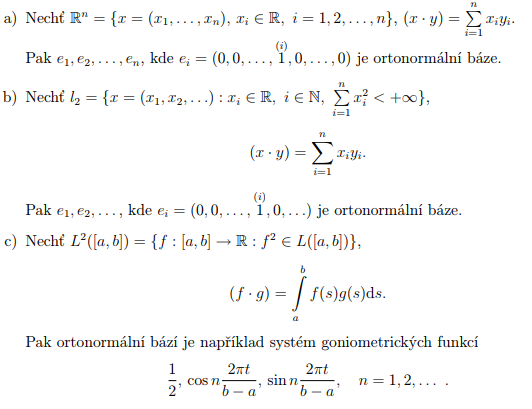
\includegraphics[width=0.8\textwidth]{Obrazky/priklady_prostoru}
\end{figure}


\section{Numerické metody řešení algebraických rovnic}  
\textit{reseni jedne nelinearni rovnice,reseni soustav nelin.rovnic,reseni soustav lin.rovnic(priame a iter.metody)}

\subsection{Riešenie soustav lineárních rovnic}  
\textit{Příme metódy} jsou takové, ktoré dodají v konečném počtu kroku přesné řešení (za predpokladu, že výpočet probíha bez zaokrouhlovacích chyb, teda zcela přesne).
\newline\textit{Iterační metódy} poskytují přibližné řešení, co je dostatoční pokud zachováme dobrou aproximaci řešení přesného. Počet kroku iterační metódy závisí na požadované přesnosti.
 \newline \newline Soustavou lin. rovnic rozumíme
\begin{align*}
a_{11} x_1 + a_{12} x_2 + \ldots + a_{1n} x_n &= b_1 \\
\ldots \\ 
a_{n1} x_1 + a_{n2} x_2 + \ldots + a_{nn} x_n &= b_n
\end{align*}
Danou soustavu je možný prepsat do tvaru $$ \sum_{j=1}^{n} a_{ij}x_j=b_i, \qquad i=1,2,...,n$$
 nebo v maticovém tvaru $$\textbf{Ax}=\textbf{b}.$$
Matici \textbf{A} nazýváme \textit{maticí soustavy}, \textbf{b} je \textit{vektor pravé strany} a  \textbf{x} je  \textit{vektor neznámých}. Budeme predpokládat, že matice soustavy je regulární, takže ťešena soustava má jediné řešení (Frobeniova veta).
 \subsection{Příme metódy}
\textbf{Gaussova eliminační metóda}

Základní příma metóda pro řešení soustav lin. rovnic je Gaussova eliminační metóda (dále GEM). Pozostáva ze dvou části-přímy a zpetný chod.
\newline V \textit{přímem chodu} GEM se soustava lin. rovnic převede na ekvivalentní soustavu $$\textbf{Ux}=\textbf{c},$$ kde \textbf{U} je tzv. \textit{horní trojuhelníková matice}, což je matice, ktorá má pod hlavní diagonálou všechny prvky nulové, tj. $u_{ij}=0$ pro $i\succ j$.
\newline     
$$U=\left( 
\begin{array}{ccc c r}
    u_{11} & u_{12} & u_{13} & ... & u_{1n} \\
    0 & u_{22} & u_{23} & ...  & u_{2n} \\
    0 & 0 & u_{33} & ... & u_{3n} \\
   \vdots & \vdots & \vdots & \vdots & \vdots \\
    0 & 0 & 0 & ... & u_{nn} \\ 
    \end{array} 
\right)$$


V \textit{zpetném chodu} se pak řeší soustava $$\textbf{Ux}=\textbf{c}.$$ Protože \textbf{A} je regulární, \textbf{U} je také regulární,z čeho vyplýva, že diagonální prvky jsou ruzne od nuly. Díky tomu vypočteme z poslední rovnice $x_{n}$, z předposlední $x_{n-1}$, atd.
\textbf{Přímy chod GEM}
Přímy chod má \textit{n-1} kroku (matice \textbf{A} má řád n). Matice \textbf{A} se mění každým krokem a to stejné vektor \textbf{b} co v k-tém kroku značíme $\textbf{A}^{(k)}$. V \textit{k-tém} kroku se snažíme vynulovat poddiagonální koeficienty v \textit{k-tém} sloupci matice $\textbf{A}^{(k)}$. Dosáhneme to tak, že od i-té rovnice odečteme $\textit{m}_{ik}$ násobek k-té rovnice lineární soustavy ($i\succ k$, protože jenom poddiagonální prvky)
$$a_{ik}^{(k)}-m_{ik}a_{kk}^{(k)}=0 \implies m_{ik}=\frac{a_{ik}^{(k)}}{a_{kk}^{(k)}}.$$
$a_{kk}^{(k)}$ se nazýva hlavní prvek nebo pivot-pokud se rovná nule, algoritmus zhavaruje (využitelný pouze když A je ryze diagonálne dominantní nebo pozitivne definitní).
\newline Tento algoritmus nevyužíva výběr hl.prvku (je braný diag.prvek), je však možní použít úplný výběr hlavního prvku nebo částeční výběr (většinou se používá částečný, kt. má menší počet operací a zaokrouhlovací chyby jsou stále dostatočne malý).
\newline 
\textit{Částečný výběr hl.prvku} v k-tém kroku eliminace se jako hl.prvek vybíra prvek s největši abs.hodnotou v zatím nezelimenované částí k-tého sloupca matice $\textbf{A}^{(k-1)}$ (prohodí se k-tý a r-tý řádek, $r\succ k$). Při \textit{Úplném výběru hl.prvku} se prohozují řádky i sloupce matice.
\newline GEM s částečným/úplným výběrem hl.prvku jsou dobře podmínené algoritmy za predpokladu, že matice soustavy je dobře podmíněná (protože velikost multiplikátoru nepřesahuje jedničku, vznikajíci zaokrouhlovací chyby se dalším výpočtem "nezesilují"). (asi by bolo vhodné niečo dodať o normách matíc a číslu podmíneností matic)
\textbf{LU rozklad}
Po ukončení přimého chodu dostaneme soustavu $\textbf{Ux}=\textbf{c}.$ Multiplikátory umístnime do dolní trojuhelníkové matice L.
$$
\bigg{[} l_{ik}= 
\begin{cases}
       0, & \text{pro } i=1,2,...,k-1 \\
       1, & \text{pro } i=k \\
        m_{ik}, & \text{pro } i=k+1,k+2,...,n
\end{cases}
\bigg{]}
$$

Platí: \textbf{A}=\textbf{LU}
\newline \textbf{Nasledujíci kroky:}
\newline 1) vypočteme soustavu $\textbf{Ly}=\textbf{b}$ pro neznámou y 
\newline 2) vypočteme soustavu $\textbf{Ux}=\textbf{y}$ pro neznámou x
\newline 3) soustava $\textbf{Ax}=\textbf{b}$ je ekvivalentní soustavě $\textbf{LUx}=\textbf{b}.$, takže x z 2) je naše řešení
\newline LU rozklad s částečným výběrem hl.prvku je založen na nájdení takových matic U (horní troj.matice),L (dolní troj.matice), P(permutační matice),že platí $\textbf{LU}=\textbf{PA}.$

\textbf{Choleského rozklad}
Platí: $\textbf{A}=\textbf{L}\textbf{L}^{T}$, kde \textbf{L} je dolní troj. matice jejíž prvky jsou ale definovane jinak než v u LU rozkladu. Postup pokračuje 1)-3) pro $\textbf{U}=\textbf{L}^{T}.$
\newline
\subsection{Iterační metódy}
Soustavu $\textbf{Ax}=\textbf{b}$ řešíme zvolením počátečního vektoru $\textbf{x}_{0}$ a generovaním posloupností vektoru $\textbf{x}_{1},\textbf{x}_{2}$,atd které konvergují k hlednanému řešení $\textbf{x}$. 
\newline\textbf{Konvergence}
\newline
řekneme, že iterační metóda konverguje, a píšeme $\textbf{x}_{k} \rightarrow\textbf{x}$, když  $\left\Vert\textbf{x}_{k}-\textbf{x}\right\Vert\rightarrow 0$. Chybu v k-té iteraci značíme $\textbf{e}_{k}=\textbf{x}_{k}-\textbf{x}$. Konvergence iterační metody z libovolného startovacího vektoru nastane, když konvergenční matice $\textbf{T}$ splňuje $\left\Vert\textbf{T}\right\Vert<1$, tahle podmínka se však neověřuje lehce.\newline Iterační metóda se ukončí když $\textbf{x}_{k}$ je dostačujíci aproximace \textbf{x}. Jedním z nejčastejších kritériií pro ukončení iterační metódy je  $\left\Vert\textbf{x}_{k+1}-\textbf{x}_{k}\right\Vert\leq \epsilon\left\Vert\textbf{x}_{k}\right\Vert$ pro dostatečne malé $\epsilon$.

\textbf{Jacobiova metoda}
\newline Matici \textbf{A} rozložíme ako \textbf{A}=\textbf{L+U+D}, kde\textbf{D} je diagonální matice, ktorá má stejnou diagonálu jako \textbf{A}, a kde \textbf{L}/\textbf{U} je ryze dolní/horní trojuholníková část matice \textbf{A}. Posloupnost vektoru $\textbf{x}_{k}$ je dána vztahem $$\textbf{D}\textbf{x}_{k+1}=\textbf{b}-\textbf{(L+U)}\textbf{x}_{k}.$$ Jacobiova metóda konverguje, když \textbf{A} je ryze diagonálně dominantní.

\textbf{Gauss-Seidelova metoda}\newline
Protože v Jacobiovej metode počítáme prvky vektoru  $\textbf{x}_{k+1}$ postupně jeden za druhým, vznikl nápad ihned využít ty složky  $\textbf{x}_{k+1}$, které jsou uz k dispozicií. Tak dostávamé Gauss-Seidlovu metodu. $$\textbf{(D+L)}\textbf{x}_{k+1}=\textbf{b}-\textbf{U}\textbf{x}_{k}.$$ MEtóda konverguje, když \textbf{A} je ryze diagonálně dominantní nebo pozitivne definitní. 
\newline Konvergence Gauss-Seidelovy metody je pro mnohé matice \textbf{A} rychlejší.

\textbf{Relaxační metody}\newline
Bezprostředně po vypočtení i-té složky v k+1 iteraci vektoru  $\textbf{x}_{k+1}$ provedeme její modifikaci $$\textbf{x}^{(k+1)}_i=(1-\omega)\textbf{x}^{(k)}_i+\omega\textbf{x}^{(k+1)}_i.$$
Relaxační parametr $\omega$ je volený tak, abychom vylepšili konvergenci základní metódy. Zvolíme-li $\omega=1$ dostávamé puvodní metodu, pro $\omega<1$ hovoříme o dolní relaxaci, v případě $\omega>1$ o horní relaxaci. Volba $\omega$ závisí na zvolené základní metodě a na matici soustavy $\textbf{A}$.

Inou známou iterační metodou je například metoda sdružených gradientu.
\subsection{Riešenie jednej nelineárnej rovnice}  
\subsection{Riešenie sústavy nelineárnych rovníc}  

\section{Interpolace a aproximace, numerické derivování a integrování}  

Aproximovat funkci $f(x)$ znamená nahradit ji funkcí $\varphi(x)$, která je k $f(x)$ v jistém smyslu blízká. Píšeme $\varphi(x)\approx f(x)$. Dva základní typy aproximace jsou interpolace a metoda nejmenších čtverců.

\textit{Interpolace} je aproximace, při níž $\varphi(x)$ nabývá v zadaných bodech $x_i$ předepsaných hodnot $y_i=f(x_i)$, někdy navíc žádáme, aby funkce $\varphi(x)$ a $f(x)$ měli v bodech $x_i$ také stejné derivace.

\textit{Metoda nejmenších čtverců} je aproximace, při níž $\varphi(x)$ "prokládáme" mezi zadanými body $[x_i,y_i]$ tak, aby "vzdálenost" funkcí $f$ a $\varphi$ byla v jistém smyslu minimální. Je přitom charakteristické, že funkce $\varphi$ neprochází body $[x_i,y_i]$.

\subsection{Interpolace}
Interpolační funkci $\varphi(x)$ vybíráme z vhodné třídy funkcí. Omezíme se na dva případy:
\begin{itemize}
\item  $\varphi(x)$ je polynom 
\item $\varphi(x)$ je po částech polynom, na každém subintervalu obecně jiný.
\end{itemize} 
\textbf{Interpolace polynomem}
Je zadáno $n$ navzájem různých bodů $x_0,x_1,...,x_n$, které nazýváme \textit{uzly interpolace} a v každém z nich je předepsaná hodnota $y_i$. Hledáme interpolační polynom $P_n(x)$ stupně nejvýše $n$, který splňuje interpolační podmínky $$P_n(x_i)=y_i,\quad i=0,1,...,n$$


\textbf{Lagrangeův tvar interpolačního polynomu}
$$P_n(x)=y_0l_0(x)+y_1l_1(x)+\ldots+y_nl_n(x)=\sum_{i=0}^{n}y_il_i(x),$$
kde $l_i(x)$ jsou tzv. fundamentální polynomy definované $$l_i(x)=\frac{(x-x_0)(x-x_1)...(x-x_{i-1})(x-x_{i+1})...(x-x_n)}{(x_i-x_0)(x_i-x_1)...(x_i-x_{i-1})(x_i-x_{i+1})...(x_i-x_n)}$$ z čeho vyplývá
\[
    l_i(x_k)= 
\begin{cases}
        1, & \text{pro } k=i\\
        0, & \text{pro } k\neq i
\end{cases}\quad  i,k=0,1,...,n,\\
\]
takže interpolační podmínky $P_n(x_k)=\sum_{i=0}^n y_il_i(x_k), \, k=0,1,\ldots,n$, jsou splněny. Interpolační polynom je daty $[x_i,y_i],\, i=0,1,\ldots, n$ určen jednoznačně, jelikož jsou-li $P$ a $Q$ interpolační polynomy splňující interpolační podmínky $P(x_i)=Q(x_i)=y_i$, pak polynom $P-Q$ je roven nule v uzlech $x_0,x_1,\ldots,x_n$ což je ve sporu s faktem, že polynom stupně $n$ může mít maximálně $n$ kořenů, pokud se nerovná identicky $0 \Rightarrow P-Q=0 \Rightarrow P=Q$. 
\newline Výhodou je jeho elegantní forma, hlavní nedostatky 
\begin{itemize}
\item Přidáme-li další uzel $x_{n+1}$, musíme přepočítat všechny fundamentální polynomy
\item Počet operací potřebných k výpočtu $P_n(\hat{x}) $ je poměrně značný, vyžaduje $2n^2+2n$ násobících operací a $2n^2+3n$ operací sčítacích.
\end{itemize}


\textbf{Newtonův interpolační polynom}\newline
Odstraňuje oba nedostatky Lagrangeového interpolačního polynomu.$$P_n(x)=a_0+a_1(x-x_0)+a_2(x-x_0)(x-x_1)+...+a_n(x-x_0)(x-x_1)...(x-x_{n-1})$$. Při přidání dalšího uzlu ostáva puvodní tvar interpolačního polynómu stejný a jenom se přičte nový člen. Koeficienty $a_i$ je možné vypočítat přímo z interpolačních podmínek nebo pomocí poměrné diference (lepší zpusob).

Poznámka k oběma interpolačným polynomum:Obecně nelze doporučit používaní interpolačních polynomu vysokých stupňu (jsou funkce, kde chyba interpolace raste s roustoucím počtem uzlu, Rungeova funkce), efektívnejší by bylo vhodne zormístnit uzly, avšak tuto možnost však obvykle nemáme, neboť uzly jsou pevně dané.

\textbf{Hermitova interpolace}\newline
Hlavní rozdíl pozostáva v tem, že interpolační polynom určují navíc také prědepsané derivace v uzlech. 
\newline
Nechť je každém uzlu zadáno $\alpha_i+1$ čísel $y_i^{(0)},y_i^{(1)},...,y_i^{(\alpha_i)}$. Označme $\alpha=n+\sum_{i=0}^n \alpha_i$. Pak Hermitovým interpolačním polynomem $P_alpha(x)$ nazveme polynom stupně nejvýše $\alpha$, který splňuje interpolační podmínky $$\frac{d^j}{dx^j}P_\alpha(x_i)=y_i^{(j)}\qquad j=0,1,...,\alpha_i,\quad i=0,1,...,n$$Je dokázáno, že existuje jediný takový polynom. Stejně jako u předchozích ani tady nelze obecně odporučit použití vysokého stupně polynomu.

\subsection{Interpolační splajny}
Když chceme interpolovat funkci $f(x)$ na poměrně dlhém intervalu $\langle a,b \rangle$, je vhodnejší nepoužívat interpolační polynomy vyšších stupňu ale interval rozdělit na řadu menších subintervalu a na každém z nich sestrojit interpolační polynom nižšího stupně. 
$$a=x_0 < x_1 < ... < x_{i-1} < x_{i} < {i+1} <...< x_{n-1} < x_n=b$$ je dělení intervalu $\langle a,b \rangle$. V každém uzlu $x_i$ je prředepsána hodnota $y_i$ interpolantu. Délka i-tého intervalu je $\langle x_{i-1},x_i \rangle$.
\subsection{Metoda nejmenších čtvercu}
\subsection{Numerické derivování}
\subsection{Numerické integrování}


\section{Numerické metody řešení počátečních problémú pro ODR}
Máme počáteční problém
\begin{align}
y'&=f(t,y(t)), \quad t \in [t_{0}, T], \\
y(t_{0})&=y_{0}
\end{align}
obecně je tento problém vektorový ($f:[t_{0},t_{f}]:\times\R ^{m} \rightarrow \R^{m}, \: y:\R \rightarrow \R ^{n}$, $y_{0}$ je vektor s m složkami) - jedná se tedy o soustavu.  Předpokládáme že problém je "well-defined", tj. řešení existuje a je jednoznačné (funkce $f$ je spojitá a  Lipschitzovská), a že existují derivace až do řádu, který budeme potřebovat. 

Rovnice vyšších řádů lze převést na soustavu rovnic prvního řádu. Proto nám stačí numerické metody pro řešení soustav rovnic prvního řádu.  

Analýza numerické metody je jednodušší pro skalární úlohu (rovnici), proto v následujícím bude vše děláno pro rovnici (stejně jako ve skriptech). 
\subsection{Základní pojmy}
\subsubsection*{Numerické řešení}
Numerické řešení jsou přibližné hodnoty hledaného řešení v bodech $t_{n}$, tj. posloupnost hodnost  $y_{0}, y_{1}, y_{2},...,y_{N}$. 

Interval $[t_{0}, T]$ na  kterém řešíme rovnici rozdělíme na N "dílků"
\begin{align}
t_{0} <  t_{1}< ... < t_{N} \leq T. 
\end{align} 
Hodnoty $t_{n}$ nazyvame \textbf{uzly}. 
Vzdálenost mezi dvěma uzly $t_{n}, t_{n+1}$ nazveme \textbf{délka kroku}: $h_{n}=t_{n+1}-t_{n}, \: n=0,1,...N-1$. Pokud jsou všechny délky kroku stejné $h_{n}=h,\; \forall n$ mluvíme o \textbf{rovnoměrném (ekvidistantním) dělení} a  platí vztahy
\begin{align}
h_{n}=h= \frac{T-t_{0}}{N}, \quad t_{n}=t_{0}+nh, \: n =0,1,...,N,
\end{align}
Pro získání řešení v jiných bodech než v uzlech musíme použít nějaký druh interpolace. 

\textbf{Značení:} \\
$y(t_{n})$ -- hodnota přesného řešení v bodě $t_{n}$ \\
$y_{n}$ -- hodnota aproximovaného (přibližného) řešení v bodě $t_{n}$

\subsubsection*{Numerická metoda}
Numerická metoda je předpis (algoritmus) pro postupný výpočet aproximací řešení   $y_{0}, y_{1}, y_{2},...,y_{N}$.

Krokem metody nazveme "přechod" od hodnoty $y_{n}$ k hodnotě $y_{n+1}$. \textbf{K-krokovou metodou} pak nazýváme metodu pro kterou výpočet $y_{n+1}$ závisí na \textit{k} předchozích aproximacích. Konkrétně pro jedno-krokovou metodu, $y_{n+1}$ závisí pouze na aproximaci $y_{n}$.

\subsection{Eulerovy metody a další pojmy numerické analýzy}
\subsubsection*{Explicitní Eulerova metoda}
  (dopředná eulerova metoda, anglicky: Euler method, explicit Euler method, forward Euler method)

Jedno z možných odvození je z Taylorova rozvoje
\begin{align}
y(t_{n+1}) = y(t_{n}+h)= y(t_{n})+hy'(t_{n}) + \frac{1}{2} h^{2} y''(\xi_{n}), \quad \xi_{n} \in (t_{n}, t_{n+1}).
\end{align}
Derivaci $y'$ nahradíme z rovnice $y'(t_{n})=f(t_{n},y(t_{n}))$ a když zanedbáme clen $\frac{1}{2} h^{2} y''(\xi_{n})$ dostaneme
\begin{align}
y(t_{n+1}) \approx y(t_{n})+h f(t_{n},y(t_{n})).
\end{align}
Přesné hodnoty $y(t_{n}), \, y(t_{n+1})$ nahradíme aproximovanými $y_{n}, y_{n+1}$ a dostaneme předpis Eulerovy metody
\begin{align}
y_{n+1}= y_{n} + hf(t_{n}, y_{n}).
\end{align}
Výpočet $y_{n+1}$ závisí pouze na jedné předchozí hodnotě aproximovaného řešení, tedy je to jednokroková metoda. Hodnota $y_{n+1}$ je určena explicitně, jedná se tedy o explicitní metodu. 

\subsubsection*{Chyby}
\textbf{Lokální diskretizační chyba} - $lte$ (local truncation error) je chyba, které se dopustíme v jednom kroku za předpokladu že $y_{n}$ je přesné řešení počáteční úlohy v čase $t_{n}$, tj. $y_{n}=y(t_{n})$:
\begin{align}
lte_{n}= y(t_{n+1})-y(t_{n})-h f(t_{n},y(t_{n})).
\end{align}
Z Taylorova rozvoje o kousek výš plyne, že $lte_{n}=\frac{h^{2}}{2} y''(\xi_{n})$ tedy $\vert lte_{n} \vert \leq C h^{2}$, kde $C=\frac{1}{2} \mathrm{max}_{t_{n}\leq t \leq t_{n+1}} \vert y''(t) \vert $. To je všechno moc pěkný - hlavní je, že lokální diskretizační chyba je úměrná velikosti kroku na druhou což označujeme pomocí Landauova symbolu jako $\mathcal{O}(h^{2})$.

Reálně tahle chyba nevzniká, protože předpoklad $y_{n}=y(t_{n})$ není obecně splněn (je splněn v prvním kroku a to jen pokud máme k dispozici přesnou počáteční podmínku). Tato chyba se tedy uplatňuje pouze při analýze vlastností metody.  

\textbf{Lokální chyba} - $le$ (local error)  je skutečná chyba které se dopustíme při reálném výpočtu v kroku od $t_{n}$ do $t_{n+1}$. S touto chybou pak pracujeme např. při řízení délky kroku.  $Le$ definovaná předpisem
\begin{align}
le_{n}=u_{n}(t_{n+1})-y_{n+1}
\end{align}
kde $u_{n}(t)$ je tzv. lokalni reseni pocatecniho problemu
\begin{align}
u'(t)=f(t,u_{n}(t)), \quad u_{n}(t_{n})=y_{n}.
\end{align}
Pokud zvolíme dostatečně malou délku kroku je rozdíl mezi $lte$ a $le$ prakticky zanedbatelný. 

\textbf{Globální diskretizační chyba} - $e$ (global truncation error) vzniká hromaděním lokálních chyb. 
\begin{align}
e_{n}= y(t_{n})-y_{n}.
\end{align}
Pro rovnoměrný dělení lze dokázat 
\begin{align}
\vert e_{n} \vert = \vert y(t_{n})-y_{n} \vert \leq C h,
\end{align}
což můžeme zase zapsat pomoci $\mathcal{O}(h)$ a řekneme, že Eulerova metoda je řádu (řádu přesnosti) 1. 

\textbf{Zaokrouhlovací chyby} asi nejsou žádným velkým překvápkem. Pokud tyto chyby nepřesáhnou $\varepsilon$ pak po $N$ krocích délky $h$ velikost nepřesáhne $K \varepsilon h^{-1}$, kde $K$ je konstanta nezávislá na $\eps$ a $ h$. Pak celková chyba $\approx Ch+ \eps K h^{-1}$. Reálně jsou zaokrouhlovací chyby malé takže pokud nepočítáme pro velmi velký počet kroků nemusí nás to nijak obtěžovat. 

\subsubsection*{Stabilita}
Počáteční problém
\subsubsection*{Implicitní Eulerova metoda}
Když opět vyjdeme z Taylorova rozvoje
\begin{align}
y(t_{n+1}-h)= y(t_{n}) = y(t_{n+1}) -hy'(t_{n+1})+ \frac{h^{2}}{2} y'' (\xi_{n}), \quad \xi_{n} \in (t_{n},t_{n+1}),
\end{align}
vypustíme člen $\frac{h^{2}}{2} y'' (\xi_{n})$ a použijeme rovnost $y'(t_{n+1})=f(t_{n+1},y(t_{n+1)}$, zaměníme přesné a aproximované hodnoty, dostaneme \textit{implicitní Eulerovu metodu}:
\begin{align}
y_{n+1}=y_{n}+h f(t_{n+1},y_{n+1}).
\end{align}
Hodnota $y_{n+1}$ je nyní dána implicitně rovnicí výše. Pro její určení musíme řešit obecně nelineární rovnici. 

Lokální diskretizační chyba je z Taylorova rozvoje výše  $\mathcal{O}(h^{2})$ a podobně jako u explicitní Eulerovy metody lze určit globální diskretizační chybu $\mathcal{O}(h)$. Obě Eulerovy metody jsou tedy řádu 1. 

Stabilita: 

vnějšek jednotkového kruhu se středem v bodě $[1,0]$. 

\subsubsection*{Lichoběžníková metoda}
Lichoběžníkovou metodu lze získat jako aritmetický průměr explicitní a implicitní Eulerovy metody:
\begin{align}
y_{n+1}= y_{n}+ \frac{1}{2} \left( f(t_{n},y_{n}) + f(t_{n+1},y_{n+1} \right).
\end{align}
$lte_{n} = \mathcal{O}(h^{3})$, $e_{n}= \mathcal{O}(h^{2})$ tj. metoda řádu 2. Oblast absolutní stability obsahuje celou zápornou polorovinu komplexní roviny. Interval absolutní stabilit je celá záporná reálná poloosa.  

\subsection{Explicitní Runge-Kuttovy metody}
Runge-Kuttovy (RK) metody jsou jednokrokové metody. S-stupňová explicitní RK metoda je určena předpisem
\begin{align}
k_{1}&= f(t_{n}, y_{n}) \\
k_{2}& = f(t_{n}+c_{2} h, y_{n} + a_{21} h k_{1}) \\
k_{3} &= f(t_{n}+c_{3} h, y_{n} + a_{31} hk_{1} + a_{32}h k_{2}) \\
\vdots& \\
k_{s} & = f(t_{n}+c_{s} h, y_{n} + a_{s1}h k_{1} + ... + a_{s, s-1}h k_{s-1})\\
y_{n+1}&= y_{n} + h(b_{1}k_{1}+b_{2}k_{2} + ...+ b_{s}k_{s}).
\end{align}
Koeficienty $k_{i}$ se nazývají  stupně. Koeficienty $a_{ij}, b_{i}, c_{i}$ určují konkrétní metodu. Lze je zapsat do tzv. Butcherovy tabulky:
\begin{center}  
 \begin{tabular}{r|r}
  $\textbf{c} $ & $\textbf{A} $ \\ \hline
  & $\textbf{b}^{T}$
   \end{tabular}
   \end{center}
   která pro explicitní metody vypadá následovně
   \begin{center}
 \begin{tabular}{l|lllll} 
   $0$      &     $0$        \\
  $ c_{2}$    &  $a_{2,1}$      &         \\
    $c_{3}$    &  $a_{3,1}$      &  $a_{3,2}$       & \\

    $\vdots$      & $\vdots $ & $\vdots$        \\
   $c_{s}$     &  $a_{s,1}$     &  $a_{s,2}$    & $\cdots$ &  $a_{s,s-1}$  &   \\\hline
    &$ b_{1}$        &$ b_{2}$  & $\cdots$   & $b_{s-1}$      & $b_{s} $\\      
  \end{tabular}  
\end{center}
První řádek, kde jsou jen nuly se někdy (třeba ve skriptech) vypouští. 

Stupně $k_{i}, i=1...,s,$ jsou směrnicí lokálního řešení procházejícího bodem $[t_{i}^{*},y_{i}^{*}]$, kde
\begin{align}
t_{i}^{*} = t_{n}+h c_{i}, \quad y_{i}^{*} = y_{n} +  a_{i1}h k_{1} + ... + a_{i, i-1}h k_{i-1}, \quad i=1,...,s.
\end{align}
Output $y_{n+1}$ je pak obdržen za pomoci lineární kombinace stupňů. Přesněji řečeno váženého průměru, protože součet všech $b_{i}$ je roven 1.

Pro odvození konkrétní metody si nejprve určíme počet stupňů metody. Poté vybereme koeficienty $a_{ij}, b_{i}, c_{i}$ tak aby metoda měla "dobrou" přesnost. Ta se měří pomocí lokální diskretizační chyby.\textit{ Metoda je řádu \textit{p} pokud pro lokální diskretizační chyba je řádu $\mathcal{O}(h^{p+1})$.} Pomocí toho lze odvodit podmínky řádu:
 \begin{align*}
 \sum _{j=1} ^{s}  b_{j} &= 1 \nonumber \\
 \sum _{j=1} ^{s}  b_{j}c_{j} &= \frac{1}{2}  \nonumber \\
 \sum _{j=1} ^{s} b_{j}c_{j}^{2}  &= \frac{1}{3} \nonumber \\
 \sum_{j=1} ^{s}  \sum _{k=1} ^{j-1} b_{j}a_{jk}c_{k}  &= \frac{1}{6} \nonumber
 \end{align*}
pro řád 1 - první rovnice, pro řád 2 - první a druhá, pro řád 3 - všechny čtyři. Pro vyšší řády počet podmínek roste (docela brutálně):
\begin{center}
\begin{tabular}{l|cccccccccc}
order $p$ & 1 & 2& 3& 4& 5&6&7&8&9&10 \\ \hline
number of conditions & 1 & 2& 4& 8& 17& 37& 85& 200& 486& 1205
\end{tabular}
\end{center}
(ta tabulka je tu spíš for fun, opovažte se to někdo učit).


Navíc se většinou předpokládá podmínka (většinou = vždycky, i když nutně ji splňovat asi nemusí všechny používaný metody ji splňují)
\begin{align}
c_{i}=\sum _{j=1} ^{i-1} a_{ij},\quad i=1,...,s.
\end{align}

Metody, které mají stejný počet stupňů jako je řád metody $s=p$ je možný sestrojit jen do řádu 4. Pro vyšší přesnost už potřebujeme $s > p$. Pro řádů 5 a 6 $s \geq p+1$ a pro vyšší pak $s \geq p+2$. 

\textbf{Metoda řádu 1} - explicitní Eulerova metoda, viz výše. 

\textbf{Metody řádu 2} - z podmínek řádu dostaneme, že koeficienty a,b jsou svázány podmínkou $b= \frac{1}{2a}$ pro $a\neq 0$. 
\begin{center}
\begin{tabular}{c|cc}
a & a \\ \hline
& 1-b & b
\end{tabular}
\end{center}
Těchto metod je kupa (dokonce nekonečně mnoho), takže takový ty proflákláknutý  který by bylo dobrý znát: \\
$a=\frac{1}{2}$ - modifikovaná Eulerova metoda, první modifikace Eulerovy metody (angl. midpoint Euler formula, explicit midpoint formula) \\
$a= 1$ - druha modifikace Eulerovy metody, Heunova metoda (angl. improved Euler method, Heun method) \\
$a=\frac{2}{3}$ - Ralstonova metoda 2. řádu. 

\textbf{Metody řádu 3} - např. Ralstonova metoda 3. řádu (základ metody Bogacki-Shampine o který bude řeč za dva/tři odstavce).

\textbf{Metody řádu 4} - nejznámější je klasická Runge-Kuttova metoda ("the" Runge-Kutta method, odvozená samotným W. Kuttou), super jednoduchá, má krásný koeficienty, proto byla dost populární před počítačové éře. Dneska už se používá spíš z nostalgie. 

\subsubsection*{Řízení délky kroku}

\subsubsection*{Odhad lokální chyby}
- Bogacki-Shampine 3(2), Dormand-Prince 5(4), Runge-Kutta-Fehlberg 4(5) \\
- metody s lokální extrapolací, FSAL property

\subsubsection*{Stabilita Runge--Kuttových metod}
Pokud řešíme testovací rovnici $y'=\lambda y,\; y(0)=1$ (viz u Eulerovy metody) RK metodou na rovnoměrném dělení s krokem $h$ dostaneme
\begin{align}
y_{n+1}=P_{s}(h \lambda) y_{n}
\end{align}
kde $P_{s}$ je polynom stupne s, určený pomocí konstant $b_{i}, a_{ij}$. Podmínka stability platí pouze pokud $h \lambda$ leží v oblasti absolutní stability $R_{A}$:
\begin{align}
h \lambda \in R_{A} = \lbrace z \in \mathbf{C} : \vert P_{s}(z) \vert < 1 \rbrace.
\end{align}
\textit{Explicitní RK metody mají omezenou oblast absolutní stability.} 

\subsection{Lineární mnohokrokové metody}
Tyto metody počítají přibližné řešení $y_{n+1}$ v uzlu $t_{n+1}$ z již spočtených aproximací $y_{n}, y_{n-1}, y_{n-2},...$ a odpovidajicich hodnot prave strany diferencialni rovnice. Tyto hodnoty jiz mame vypocteny, tedy pro ziskani $y_{n+1}$ s vysokou presnosti potrebujeme  jen malo novych vyhodnoceni prave strany. 

Predpis obecne linearni k-krokove metody:
\begin{align}
\alpha_{0} y_{n+1} + \alpha_{1} y_{n} + ... + \alpha_{k} y_{n+1-k} = h \left( \beta_{0} f(t_{n+1},y_{n+1})+ ... + \beta_{k}f(t_{n+1-k},y_{n+1-k}) \right)
\end{align}
Koeficienty $\alpha_{j}, \beta_{j}$ urcuji konkretni metodu. \\
Predpokladame normalizacni podminku $\alpha_{0}=1$ \\
Pokud $\alpha_{k} \neq0$ nebo $\beta_{k} \neq 0$ pak je metoda k-krokova \\
Pro $\beta_{0} \neq 0$ - implicitni metoda \\
Pro $\beta_{0}= 0 $ - explicitni metoda \\
Pro k-krokovou metodu potrebujeme $k-1$ startovacich hodnot $y_{0},y_{1},...y_{k-1}$, $y_{0}$ z pocatecni podminky, $y_{r}, r<k$ pomoci nejvyse r-krokove metody. 

\textbf{D-stabilita}
Řekneme, že metoda je stabilní ve smyslu Dahlquista (D-stabilní) jestliže všechny kořeny prvního charakteristického polynomu $\rho (\xi) = \xi^{k} + \alpha_{1} \xi^{k-1}+...+\alpha_{k-1} \xi+ \alpha_{k}$ leží uvnitř jednotkového kruhu $\vert z \vert < 1$ komplexni roviny $\mathbb{C}$ a pokud nektery koren lezi na hranici pak je jednoduchy. 

\textbf{Konvergence}
Uvažujeme D-stabilní lineárni mnohokrokovou metodu řádu $p \neq 1$ . Jestliže startovací hodnoty zadáme s chybou řádu $\mathcal{O}(h^{p})$ , pak globální diskretizační chyba je rovněž řádu $\mathcal{O}(h^{p}) $.

\textbf{Absolutni stabilita} = A-stabilita \\
Máme testovací úlohu (stejne jako pro RK metody)
\begin{align}
y'&=\lambda y \\
y_{0}&=1
\end{align}
na rovnomernem deleni pak pro linearni mnohokrokovou metodu dostaneme
\begin{align}
\sum_{j=0}^{k} (\alpha_{j} - h \lambda \beta_{j}) y_{n+1-j}=0
\end{align}
řešení pak hledáme ve tvaru $y_{n}=r^{n}$. Dosazenim do rovnice o kousek vys dostaneme
\begin{align}
\sum_{j=0}^{k}(\alpha_{j}-h \lambda \beta_{j})r^{n+1-j} = r^{n+1-k} \sum _{j=0}^{k} (\alpha_{j}-h \lambda \beta_{j}) r^{k-j}=r^{n+1-k} \pi (r,h\lambda) =0
\end{align}
kde 
\begin{align}
\pi(\xi,z) = \sum _{j=0}^{k}(\alpha_{j}-z \beta _{j}) \xi^{k-j}
\end{align}
je polynom stability. Oblast absolutni stability pro linearni mnoho krokove metody pak definujeme jako mnozinu bodu komplexni rovniny pro ktere kazdy koren $\xi$ polynomu stability $\pi(\xi, z)$ lezi uvnitr jednotkoveho kruhu komplexni roviny, $\vert \xi\vert<1$. A podminka stability plati pro $z$ z oblasti absolutni stability. 


\subsubsection*{Adamsovy metody}

Vezmu diferencialni rovnici
\begin{align}
y'(t)= f(t,y(t))
\end{align}
a zintegruju ji od $t_{n}$ do $t_{n+1}$
\begin{align*}
y(t_{n+1})-y(t_{n}) = \int \limits_{t_{n}}^{t_{n+1}} f(t,y(t) \mathrm{d}t
\end{align*}
Funkci $f(t,y(t))$ aproximujeme pomoci interpolacniho polynomu $P_{k-1}(t)$ stupne $k-1$ (Líba nepíše jakýho, lepší zdroje uvádí Langrangeův) tož tedy
\begin{align}
y(t_{n+1}) \approx y(t_{n}) + \int \limits _{t_{n}}^{t_{n+1}} P_{k-1}(t) \mathrm{d}t
\end{align}
kde hodnota iterpolacniho polynomu v uzlu interpolace je rovna funkcni hodnote prave strany diferencialni rovnice tj.:
\begin{align}
P_{k-1}(t_{n+1-j}) = f(t_{n+1-j},y(t_{n+1-j})).
\end{align}
Pak uz jen pribliznou rovnost nahradime rovnosti a presna reseni nahradime pribliznym resenim a voilà:
\begin{align}
y_{n+1}=y_{n}+ \int \limits _{t_{n}}^{t_{n+1}} P_{k-1}(t) \mathrm{d}t.
\end{align}

\textbf{Adams-Bashfothovy metody}
\\ dostanu ze vztahu vyse pro $j=1,2,..,k$. \\
Lze ji tedy zapsat jako \begin{align}
 y_{n+1}=y_{n} + h \sum _{j=1}^{k} \beta^{*}_{k,j} f(t_{n+1-j}, y_{n+1-j}),
\end{align}
kde koeficienty lze najit v tabulce ve skriptech nebo urcit z formule taktez ve skriptech (kdyby to nahodou nekoho zajimalo). 
 \\
D-stabilni \\
k-krokova  řádu k\\
AB1 je eulerova metoda \\

\textbf{Adams-Moultonovy metody}\\
dostanu ze vztahu vyse pro $j=0,1,2,..,k-1$. \\
Lze ji tedy zapsat jako \begin{align}
 y_{n+1}=y_{n} +h \beta_{k,0} f(t_{n+1},y_{n+1})+ h \sum _{j=1}^{k-1} \beta_{k,j} f(t_{n+1-j}, y_{n+1-j}),
\end{align}
zjevně jsou to metody implicitní \\
koeficienty viz skripta (pokud to nekoho zajima) \\
D-stabilní \\
pro $k=1$ jednokroková - prvniho radu \\
pro $k > 1$ (k-1)-krokova a radu k\\
AM1 - implicitni Euler, AM2 - trapezoidal

\textbf{Metody korektor-prediktor} \\
Schema PECE, P(EC)$^{s}$E, PECLE \\
ABk-AMk-PECE
\begin{itemize}
\item \textbf{P} = predikce - spocteme hodnotu $y^{*}_{n+1}$ ABk metodou 
\item \textbf{E} = evaluace - vyhodnotime pravou stranu $f^{*}_{n+1}=f(t_{n+1,y^{*}_{n+1}})$
\item \textbf{C} = korekce - spocteme hodnotu $y^{**}_{n+1}$ AMk metodou, hodnotu $y^{*}_{n+1}$ pouzijeme jako pocitacni aproximaci pro reseni nelinearni rovnice, tim nam staci jen nekolik malo iteraci
\item \textbf{E} = evaluace - vyhodnotime pravou stranu $f^{**}_{n+1}=f(t_{n+1,y^{**}_{n+1}})$
\end{itemize}

Muzeme take pouzit dvojci metod ABk-AM(k+1)

Algoritmus PECLE obsahuje navic krok zvany lokalni extrapolace. Pro dvojice ABk-AM(k) pouzijeme Milneův odhad  chyby 
\begin{align}
est_{n}=\frac{C_{k+1}}{C^{*}_{k+1}-C_{k+1}}(y^{**}_{n+1}-y^{*}_{n+1})
\end{align}
pro dvojice ABk-AM(k+1) pouzijeme
\begin{align}
est_{n}=y_{n+1}-y^{**}_{n+1},
\end{align}
kde $y_{n+1}$ je spocteno metodou AM(k+1)

ABk-AMk-PECLE
\begin{itemize}
\item \textbf{P} = predikce - spocteme hodnotu $y^{*}_{n+1}$ ABk metodou 
\item \textbf{E} = evaluace - vyhodnotime pravou stranu $f^{*}_{n+1}=f(t_{n+1},y^{*}_{n+1}mjj)$
\item \textbf{C} = korekce - spocteme hodnotu $y^{**}_{n+1}$ AMk metodou, 
\item \textbf{L} = lokalni extrapolace - spocteme $est_{n}$,  $y_{n+1}=y^{**}_{n+1}+est_{n}$
\item \textbf{E} = evaluace - vyhodnotime pravou stranu $f_{n+1}=f(t_{n+1},y_{n+1})$
\end{itemize}

\textbf{Metody zpetne diference}
- Metody zpetneho derivovani, BDF=backward differentiation formulas \\

V diferencialni rovnici
\begin{align}
y'(t_{n+1})=f(t_{n+1},y(t_{n+1}))
\end{align}
nahradime derivaci $y(t_{n+1})$ pomoci derivace $P'_{k}(t_{n+1})$ interpolacniho polynomu (Lagrange) stupne k, prochazejiciho body $[t_{n+1},y(t_{n+1})],[t_{n},y(t_{n})], [t_{n-1},y(t_{n-1})],...., [t_{n+1-k},y(t_{n+1-k})]$. 

Pak BDF metodu piseme ve tvaru
\begin{align}
\alpha_{k,0} y_{n+1} + \sum _{j=1}^{k}\alpha_{k,j} y_{n+1-j} = h \beta _{k,0}f(t_{n+1},y_{n+1})
\end{align}
implicitni \\
k-krokova  radu k \\
D-stabilini pro $k \leq 6$ \\
BDF1 = implicitni euler \\
Mají vetší chybové konstanty nez AM metody \\
Mají neomezenou oblast absolutní stability - BDF1 a BDF 2 jsou A-stabilní = jejich oblast absolutní stability obsahuje celou zápornou reálnou polorovinu, ostatní metody jsou $A(\alpha)$-stabilní = jejich oblast absolutní stability obsahuje nekonečný klín $W_{\alpha}=\lbrace re^{i \varphi} \in \mathbb{C} | r>0, \vert \varphi - \pi \vert < \alpha \rbrace$  - obrazky zde: $https://en.wikipedia.org/wiki/Backward\_differentiation\_formula$. \\
BDF metody jsou taky L-stabilni, L$(\alpha)$-stabilni 





\subsection{Tuhe problemy}

%%%%%%%%%%%%%%%%%%%%%%%%%%%%%%%%%%%%%%%%%%%%%%%%%%%%%%%%%%%%%%%%%%%%%%%%%%%%%%%%%%%%%%%%%%%%%%%%%%%%%


\section{Prostory funkcií}

\section{Numerické metody řešení okrajových problémú ODR}
metoda střelby, diferenční metoda, metoda konečných objemů, metoda konečných prvků

\section{Numerické metody řešení PDR}
diferenční metoda, metoda konečných objemů, metoda konečných prvků



\chapter{Pravděpodobnost, statistika a zpracování digitálních obrazú}
\section{Pravděpodobnost}
\subsection{Náhodné jevy, Prostory elementárních jevů, Jevová Pole}
Symbolem $\omega$ budeme značit \textbf{elementární jev}. Elementárním jevem můžeme rozumět např. výsledek pokusu, jenž není jednoznačně určen podmínkami, za kterých se odehrává (Př.: výsledek hodu kostkou). Množinu všech elementáních jevů označujeme $\Omega$ a nazýváme ji \textbf{Prostor elementárních jevů.} (Jevové pole). Většinou se nezajímáme o jednotlivé elementární jevy ale o určité jejich množiny (Př.: Při hodu kostkou padne sudé číslo, atp.). Z matematického hlediska  je výhodné zajímat se o takový systém množin elementárních jevů, který tvoří $\sigma$-algebru.

\begin{definition}
Řekneme, že jev $A$ je elementární jev, jestliže neexistují jevy $B$ a $C$ různé takové, že $A=B\cup C$
\end{definition}

\begin{definition}\label{SihmaAlgebra}(jevová \textbf{$\sigma$-algebra})
Nechť $ \Omega $ je základní prostor přiřazený náhodnímu pokusu a $ 2^{\Omega} $ její potenční množina. Množinu $\mathcal{A} \subseteq 2^{\Omega} $ nazveme jevovou $\sigma$-algebrou, jestliže
\begin{itemize}
\item[\textit{(i)}] $ \Omega \in \mathcal{A} $.
\item[\textit{(ii)}] $\mathcal{A}$ je uzavřená na operaci doplňek, to jest, jestliže $A \in \mathcal{A}$ pak i $ A^{c} \in \mathcal{A} $.
\item[\textit{(iii)}] $\mathcal{A}$ je uzavřená na operaci spočetné sjednocení, to jest, jestliže $ \lbrace A_{n} \rbrace_{n \in \mathbb{N}} \in \mathcal{A}$ potom i $ \bigcup_{n \in \mathbb{N}}A_{n} \in \mathcal{A} $
\end{itemize}
Množina $A\in \mathcal{A} $ se nazývá jev, dvojice $(\Omega,\mathcal{A})$ jevové pole.
\end{definition}

\subsection{Axiomatická pravděpodobnost}

Naším cílem je být schopni jednotlivým množinám patřícím do $\mathcal{A}$ připisovat pravděpodobnost, t.j. chtěli bychom být schopni množiny $\mathcal{A}$ měřit. Pro zadefinování pravěpodobnostní míry budeme potřebovat následující:


\begin{definition}\label{SihmaAditivitaDef}(\textbf{$\sigma$-aditivita})
Nechť $\mathcal{A}\subset 2^{\Omega}$ a nechť $\mu : \mathcal{A} \longrightarrow [0,\infty]$ je množinová funkce. Řekneme že $\mu$ je $\sigma$ aditivní, jestliže pro libovolné $\lbrace A_{n} \rbrace_{n\in \mathbb{N}} \in \mathcal{A} $ vzájemně disjunktní, splňující $\bigcup_{n \in \mathbb{N}}\in \mathcal{A}$ platí 
\begin{equation}\label{SihmaAditivitaRce}\nonumber
\mu \bigg( \bigcup_{n \in \mathbb{N}}A_{n} \bigg) = \sum_{n \in \mathbb{N}} \mu(A_{n})
\end{equation}

\end{definition}

Nyní už můžeme definovat míru a pstní míru.

\begin{definition}\label{MiraPstniMiraDef}(\textbf{ Pravděpodobnostní míra})
Nechť $\mathcal{A} \subset 2^{\Omega}$ je $\sigma$-algebra a nechť $\mu:\mathcal{A} \longrightarrow [0,\infty]$ je množinová funkce splňující $\mu(\emptyset) = 0$. $\mu$ nazveme \textbf{pravděpodobnostní míra}, jestliže $\mu$ je $\sigma$-aditivní, a $\mu(\Omega) = 1$.
V dalším budeme pravděpodobnostní míru označovat $\mathbf{P}$.
\end{definition}

\begin{definition}\label{PstniProstor}\textbf{(Pravděpodobnostní prostor)}
\begin{itemize}
\item[(i)] Dvojice $(\Omega, \mathcal{A})$ tvořený neprázdnou množinou $\Omega$ a $\sigma$-algebrou $\mathcal{A}\subset 2^{\Omega}$ se nazývá měřitelný prostor. Množiny $A \in \mathcal{A}$ se nazývají měřitelné množiny. Jestliže $\Omega$ je nejvýše spočetně nekonečné a jestliže $\mathcal{A} = 2^{\Omega}$, pak nazveme měřitelný prostor $(\Omega, 2^{\Omega})$ diskrétní.
\item[(ii)] Trojice $(\Omega, \mathcal{A}, \mu)$ se nazývá prostor s mírou, jestliže $(\Omega, \mathcal{A})$ měřitelný prostor, a jestliže $\mu$ je $\sigma$-aditivní na $\mathcal{A}$.
\item[(iii)] Jestliže navíc $\mu(\Omega)= 1$ (viz Definici \ref{MiraPstniMiraDef} - Pstní míra), potom $(\Omega, \mathcal{A}, \mu)$ se nazývá pravděpodobnostní prostor. V tomto případě se množiny $A \in \mathcal{A}$ nazývají jevy.
\end{itemize}
\end{definition}

\begin{definition}\textbf{(Konečnost, $\sigma$-konečnost)}
Nechť $\mathcal{A}$ je $\sigma$-algebra. Množinovou funkci $\mu: \mathcal{A} \longrightarrow [0,\infty]$, která je aditivní na $A$ nazveme
\begin{itemize}
\item[(i)] \textbf{konečnou}, jestliže $\mu(A)<\infty$ pro každé $A \in \mathcal{A}$.
\item[(ii)]\textbf{$\sigma$-konečnou}, jestliže existuje posloupnost množin $\Omega_{1},\Omega_{2}, ... \in \mathcal{A}$ takových, že $\Omega = \bigcup_{n=1}^{\infty}\Omega_{n}$ , a  že $\mu(\Omega_{n})<\infty$ pro všechna $n \in \mathbb{N}$.
\end{itemize}
\end{definition}

\subsection{Vlastnosti pravděpodobnosti}\label{SubsVlastnostiPsti}
\begin{theorem} Nechť $(\Omega, \mathcal{A},\textbf{P}$ je pravděpodobnostní prostor. Pak pro libovolné jevy $A,A_1,A_2,\ldots$ má pravděpodobnost následující vlastnosti:
\begin{itemize}
\item[(i)] $\textbf{P}[\emptyset] = 0$.
\item[(ii)] $0 \leq \textbf{P}[A] \leq 1$.
\item[(iii)] Je-li $A_{1} \subseteq A_{2}$, pak $\textbf{P}[A_{1}] \leq \textbf{P}[A_{2}]$.
\item[(iv)] Je-li $A_{1} \subseteq A_{2}$, pak $\textbf{P}[A_{2} - A_{1}] = \textbf{P}[A_{2}] - \textbf{P}[A_{1}]$.
\item[(v)] $\textbf{P}[\overline{A}] = 1 - \textbf{P}[A]$.
\item[(vi)] $\textbf{P}[A_{1} \setminus A_{2}] = \textbf{P}[A_{1}] - \textbf{P}[A_{1} \cap A_{2}].$
\item[(vii)] $\textbf{P}[A_{1} \cup A_{2}] = \textbf{P}[A_{1}] + \textbf{P}[A_{2}] - \textbf{P}[A_{1} \cap A_{2}]$
\item[(viii)] 
\begin{align*}
\textbf{P}\bigg[ \bigcup_{i = 1}^{n} A_{i} \bigg] &= \sum_{i=1}^{n}\textbf{P}[A_{i}] - \sum_{i=1}^{n-1}\sum_{j=i+1}^{n}\textbf{P}[A_{i} \cap A_{j}] \\
&= \sum_{i=1}^{n-2}\sum_{j=i+1}^{n-1}\sum_{k=j+1}^{n}\textbf{P}[A_{i} \cap A_{j} \cap A_{k}]- ... + (-1)^{n-1}\textbf{P}[A_{1} \cap A_{2} \cap ... \cap A_{n}]
\end{align*}
\item[(ix)] $\textbf{P}[\bigcup_{i=1}^{n} A_{i}] \leq \sum_{i=1}^{n} \textbf{P}[A_{i}].$
\end{itemize}
\end{theorem}

\subsection{Podmíněná pravděpodobnost}
\begin{definition}\textbf{(Podmíněná pravděpodobnost)}\label{podm_pst}
Nechť $( \Omega, \mathcal{A}, \textbf{P})$ je pravděpodobnostní prostor a $A \in \mathcal{A}$. Podmíněnou pravděpodobnost  jevu $B$ za podmínky $A$ definujeme pro libovolné $B \in \mathcal{A}$ jako
\begin{equation}
\textbf{P}[B|A] = \frac{\textbf{P}[A \cap B]}{\textbf{P}[A]},
\end{equation}
za předpokladu, že $ \textbf{P}[A] > 0 $.
\end{definition}

Poznámka: \\
Uvažujme pravděpodobnostní prostor $( \Omega, \mathcal{A}, \textbf{P})$. Snadno se vidí, že pro nějaký pevně daný jev $A \in \mathcal{A}$, $\textbf{P}[A] > 0$ podmíněná pravděpodobnost $P[\cdot | A] $ splňuje $\sigma$-aditivitu a je normovaná, t.j. $\textbf{P}[\Omega | A] = 1$ a je tedy také pravděpodobnostní mírou ( = pravděpodobností) ve smyslu Definice \ref{MiraPstniMiraDef}. Důsledkem tohoto má také všechny vlastnosti axiomatické pravděpodobnosti (viz Odstavec \ref{SubsVlastnostiPsti}, nebo Skripta Michálek, str. 30).
\begin{theorem}[Výpočet pravděpodobnosti průniku]
Nechť $(\Omega,\mathcal{A},\textbf{P})$ je pravděpodobnostní prostor, $A_1,A_2,\ldots,A_n \in \mathcal{A}$ jsou takové, že $\textbf{P}(A_1\cup \ldots \cup A_n) > 0$. Pak
\begin{equation*}
\textbf{P}(A_1\cup \ldots \cup A_n) =\textbf{P}(A_1)\textbf{P}(A_2|A_1)\textbf{P}(A_3|A_1\cup A_2)\ldots \textbf{P}(A_n|A_1\cup \ldots \cup A_{n-1})
\end{equation*}
\end{theorem}

\begin{theorem}\label{PodmPSumForm}\textbf{(Sumační formule)/(Vzorec pro výpočet úplné pravděpodobnosti)} Nechť $( \Omega, \mathcal{A}, \textbf{P})$ je pravděpodobnostní prostor a $I$ je spočetná množina a nechť $(B_{i})_{i \in I}$ jsou vzájemně disjunktní množiny s $\textbf{P}[\bigcup_{i \in I}B_{i}] = 1$ (tj. tvoří rozklad množiny $\Omega$). Potom pro libovolné $A \in \mathcal{A}$ máme
\begin{equation}
\textbf{P}[A] = \sum_{i \in I}\textbf{P}[A | B_{i}]\textbf{P}[B_{i}].
\end{equation}
\end{theorem}
\begin{proof}
Díky $\sigma$-aditivitě $\textbf{P}$ máme
\begin{equation}
\textbf{P}[A] = \textbf{P}\bigg[ \bigcup_{i \in I}(A \cap B_{i} \bigg] = \sum_{i\in I} \textbf{P}[A \cap B_{i}] = \sum_{i \in I}\textbf{P}[A|B_{i}]\textbf{P}[B_{i}].
\end{equation}
\end{proof}

\begin{theorem}\label{PodmPBayes}\textbf{(Bayesova formule)}
 Nechť $( \Omega, \mathcal{A}, \textbf{P})$ je pravděpodobnostní prostor a $I$ je spočetná množina a nechť $(B_{i})_{i \in I}$ jsou vzájemně disjunktní množiny s $\textbf{P}[\bigcup_{i \in I}B_{i}] = 1$. Potom pro libovolné $A \in \mathcal{A}$ s $\textbf{P}[A]>0$ a libovolné $k \in I$ máme
\begin{equation}
\textbf{P}[B_{k}|A] = \frac{\textbf{P}[A|B_{k}]\textbf{P}[B_{k}]}{\sum_{i \in I}\textbf{P}[A|B_{i}]\textbf{P}[B_{i}]}.
\end{equation} 
\end{theorem}
\begin{proof}
Máme
\begin{equation}
\textbf{P}[B_{k}|A] = \frac{\textbf{P}[B_{k} \cap A]}{\textbf{P}[A]} = \frac{\textbf{P}[A|B_{k}]\textbf{P}[B_{k}]}{\textbf{P}[A]}.
\end{equation}
Následným využitím výrazu pro $\textbf{P}[A]$ z Věty \ref{PodmPSumForm} je tvrzení dokázáno.
\end{proof}

\subsection{Nezávislost}
\begin{definition}\label{DefJednoduchaNez}\textbf{Nezávislost jevů (Součinové pravidlo)} Nechť $( \Omega, \mathcal{A}, \textbf{P})$ je pravděpodobnostní prostor. Řekneme, že dva jevy $A,B \in \mathcal{A}$ jsou nezávislé, jestliže platí
\begin{equation}
\textbf{P}(A \cap B) = \textbf{P}(A) \cdot \textbf{P}(B).
\end{equation}
Analogicky pro více jevů, nechť $I$ je libovolná indexová množina a $(A_{i})_{i \in I}$ libovolný systém jevů. Tento systém jevů $(A_{i})_{i \in I}$ nazveme nezávislý, jestliže pro libovolnou konečnou podmnožinu $J \subset I$ platí
\begin{equation}
\textbf{P}\bigg[ \bigcap_{j \in J} A_{j} \bigg] = \prod_{j \in J} \textbf{P}[A_{j}].
\end{equation}
\end{definition}

\begin{theorem}
Nechť $( \Omega, \mathcal{A}, \textbf{P})$ je pravděpodobnostní prostor. Pak platí
\begin{enumerate}
\item když $A$ a $B$ jsou nezávislé, pak i $A$ a $\overline{B}$, resp. $\overline{A}$ a $B$, resp. $\overline{A}$ a $\overline{B}$ jsou (ve dvou) nezávislé
\item Jev nemožný a libovolný jev $A$ jsou nezávislé.
\item Jev jistý a libovolný jev $A$ jsou nezávislé
\item Když $0<\textbf{P}(B)<1$ pak platí následující tvrzení: Jevy $A$ a $B$ jsou nezávisé právě tehdy, když $\textbf{P}(A|B)=\textbf{P}(B|A)$
\end{enumerate}
\end{theorem}

\begin{theorem}
Nechť $( \Omega, \mathcal{A}, \textbf{P})$ je pravděpodobnostní prostor a náhodné jevy $A_1,\ldots,A_n \in \mathcal{A}$ jsou skupinově nezávislé. Pak platí
\begin{enumerate}
\item Každá alespoň dvouprvková podmnožina z těchto jevů je skupinově nezávislá.
\item Nahradíme-li $k$ jevů mezi $A_1,A_2,\ldots,A_n$ jejich doplňky, dostáváme $n$-tici skupinově nezávislých jevů
\item $\textbf{P}(\cup_{i-1}^{n} A_i)=1-\prod_{i-1}^{n}(1-P(A_i))$ 
\end{enumerate}
\end{theorem}


\section{Náhodná veličina}
\subsection{Definice}
Pro úplnost (a taky protože to Alčena po mně chtěla) uvedu nejprve konstrukci borelovské $\sigma$-algebry.
\begin{theorem}{(\textbf{O průniku systémů množin})}
Nechť $I$ je libovolná indexová množina, dále předpokládejme, že pro $\forall i \in I$ je $\mathcal{A}_{i}$ $\sigma$-algebra. Potom množina $$\mathcal{A}_{I} = \lbrace A \in 2^{\Omega} : A \in \mathcal{A}_{i} \quad pro \quad \forall i \in I \rbrace = \bigcap_{i \in I} \mathcal{A}_{i}$$ je $\sigma$-algebra. 
\end{theorem}
\begin{proof}
Důkaz spočívá v ukázání, že $\mathcal{A}_{I}$ splňuje vlastnosti $(i) - (iii)$ definice $\sigma$-algebry.
\begin{itemize}
\item[\textbf{(i)}] Zřejmě $\Omega \in \mathcal{A}_{i}$ pro $\forall i \in I$, jelikož $\mathcal{A}_{i}$ je $\sigma$-algebra pro $\forall i \in I$, odtud $\Omega \in \mathcal{A}_{I}$
\item[\textbf{(ii)}] Nechť $A\in \mathcal{A}_{I}$ je libovolná množina, pak $A\in \mathcal{A}_{i}$ pro $\forall i \in I$ , z vlastností $\sigma$-algebry plyne, že $A^{c}\in \mathcal{A}_{i}$ pro $\forall i \in I$, tedy $A^{c}\in \mathcal{A}_{I}$
\item[\textbf{(iii)}] Nechť $A_{1},A_{2}...\in \mathcal{A}_{I}$ jsou libovolné, pak $A_{n}\in \mathcal{A}_{i}$ pro $\forall i \in I$ a pro $\forall n \in \mathbb{N}$ , opět z vlastností $\sigma$-algebry dostáváme, že $ \bigcup_{n \in \mathbb{N}}A_{n} \in \mathcal{A}_{i} $ pro $\forall i \in I$, odtud $\bigcup_{n \in \mathbb{N}}A_{n} \in \mathcal{A}_{I}$.
\end{itemize}
\end{proof}
\begin{theorem}{(\textbf{Generovaná $\sigma$-algebra})}
Nechť $\epsilon \subset 2^{\Omega}$ je libovolné, potom existuje nejmenší $\sigma$-algebra $\sigma(\epsilon)$ obsahující $\epsilon$: $$\sigma(\epsilon) = \bigcap_{\mathcal{A} \quad je \quad \sigma-algebra, \quad \epsilon \subset \mathcal{A}}\mathcal{A}$$ 
$\sigma(\epsilon)$ se nazývá $\sigma$-algebra generovaná $\epsilon$, $\epsilon$ se nazývá generátor.
\end{theorem}
\begin{proof}
Jelikož $\mathcal{A} = 2^{\Omega}$ je $\sigma$-algebra a platí $\epsilon \subset 2^{\Omega}$, $\sigma(\epsilon)$ je neprázdná. Podle předchozí věty $\sigma(\epsilon)$ je $\sigma$-algebra. Je zřejmé, že $\sigma(\epsilon)$ je nejmenší $\sigma$-algebra obsahující $\epsilon$.
\end{proof}


\begin{definition}\textbf{(Topologie)}
Nechť $ \Omega $ je libovolná množina a $ 2^{\Omega} $ její potenční množina. Libovolnou množinu $\tau \subset 2^{\Omega} $ tvořenou pouze otevřenými množinami z $\Omega$ nazveme \textit{topologií}, jestliže splňuje následující vlastnosti:
\begin{itemize}
\item[\textit{(i)}] $ \Omega, \emptyset \in \tau $.
\item[\textit{(ii)}] Jestliže $\lbrace O_{n} \rbrace_{n \in \mathbb{N}} \in \tau$ je posloupnost otevřených množin náležící do $ \tau$, potom $\bigcup_{n \in \mathbb{N}}O_{n} \in \tau$.
\item[\textit{(iii)}] Jestliže $O_{1}, ..., O_{n} \in \tau $ jsou otevřené množiny náležící do $\tau$ potom $O_{1}\cap ...\cap O_{n} \in \tau$.
\end{itemize}
Dvojici $(\Omega, \tau)$ potom nazýváme \textit{topologický prostor}.
\end{definition}


\begin{definition}[\textbf{(Borelovská $\sigma$-algebra)}]
Nechť $(\Omega, \tau)$ je topologický prostor. Potom $\sigma$-algebra $$\mathcal{B}(\Omega)=\mathcal{B}(\Omega,\tau) = \sigma(\tau),$$ nejmenší $\sigma$-algebra generovaná topologií $\tau$, se nazývá \textbf{Borelovská} $\bm{\sigma}$ \textbf{algebra}. Její prvky $A \in \mathcal{B}(\Omega, \tau)$ se nazývají \textbf{Borelovské množiny}, nebo \textbf{Borelovské měřitelné množiny}.
\end{definition}

Představme si, že máme náhodný experiment - hod kostkou. Možné jevy jsou: "padne jednička", "padne dvojka", ... atd. Pro další zkoumání našeho experimentu bychom chtěli jednotlivým jevům přiřadit nějaké číselné ohodnocení, takovýto model by nám například umožnil výpočet číselných charakteristik jako jsou střední hodnota, rozptyl atd. Naším cílem je tedy přiřadit např. jevu "padne dvojka" číslo $2$, tedy "padne dvojka" $\longrightarrow 2$. Definujme náhodnou veličinu.
\begin{definition}{(\textbf{Náhodná veličina})}
Nechť $( \Omega, \mathcal{A}, \textbf{P}) $ je pravděpodobnostní prostor, nechť $(\mathbb{R}, \mathcal{B})$ je reálná osa a systém jejích Borelovských množin, potom měřitelné zobrazení $X: (\Omega, \mathcal{A}, \textbf{P}) \longrightarrow (\mathbb{R}, \mathcal{B}) $ nazveme náhodná veličina.
\end{definition}

Každé Borelovské možine lze přiřadit její vzor $X^{-1}(B) = \lbrace \omega \in \Omega : X(\omega) \in B \rbrace$ s pomocí $X$ (náhodná veličina je měř. zobrazení) a pravděpodobnostní míru $Q(B) = \textbf{P}\lbrace X^{-1}(B) \rbrace$.



\subsection{Distribuční funkce}
\begin{definition}{\textbf{(Rozdělení, distribuční funkce)}}
Nechť $X$ je náhodná veličina
\begin{itemize}
\item[(i)] pravděpodobnostní míru $\textbf{P}_{X} = \textbf{P} \circ X^{-1}$ nazveme zákonem rozdělení (rozdělením) náhodné veličiny $X$. Když $\textbf{P}_{X} = \mathcal{L}$ píšeme $X \sim \mathcal{L}$ a říkáme, že $X$ má rozdělení $\mathcal{L}$.
\item[(ii)] zobrazení $F_{X}: x \mapsto \textbf{P}\lbrace X < x \rbrace$ se nazývá distribuční funkce náhodné veličiny $X$.
\end{itemize}
\end{definition}
\begin{remark}
Distribuční funkce přiřazuje každému $x \in \mathbb{R}$ pomocí $X$ pravděpodobnostní míru Borelovské možiny $B = ( -\infty, x)$. 

Mezi zákonem rozdělení a distribuční funkcí je vzájemně jednoznačný vztah.
\end{remark}
\begin{remark}{\textbf{(Vlastnosti distribuční funkce)}}
Každá distribuční funkce je neklesající, zleva spojitá (zprava pokud do definičního vztahu zaměním $\leq$ za $<$), může mít jen spočetně mnoho bodů nespojitosti a platí pro ni
\begin{itemize}
\item[(i)] $\lim_{x \longrightarrow -\infty}F_{X} = 0$ a $\lim_{x \longrightarrow \infty}F_{X} = 1$.
\item[(ii)]pro libovolná reálná $x_{1}, x_{2}$ taková že $x_{1} < x_{2}$ $\textbf{P}(x_{1} < X \leq x_{2}) = F(x_{2}) - F(x_{1})$
\end{itemize} 
\end{remark}

\subsection{Diskrétní a spojité náhodné veličiny}
V matematické statistice mají největší uplatnění následující dva typy distribučních funkcí:
\begin{itemize}
\item[(a)] Distribuční funkce je funkce skoků. Potom říkáme, že má náhodná veličina $X$ diskrétní rozdělení pravděpodobnosti. Jak již bylo zmíněno, bodů nespojitosti může být jen spočetně mnoho, označme je $x_{1}, x_{2}, ...$. Nechť $p_{k}$ je velikost skoku funkce $F_{X}$ v bodě $x_{k}$. Lze ukázat, že platí $p_{k} = \textbf{P}\lbrace X = x_{k} \rbrace$.
\item[(b)] Existuje taková funkce $f(x), $ že platí
\begin{equation}\label{VyjadreniDistFce}
F(x) = \int_{-\infty}^{x}f(t)dt.
\end{equation}
\end{itemize}
Pak se jedná o spojité rozdělení pravěpodobnosti. Z teorie míry je známo, že $F_{X}$ má vyjádření \eqref{VyjadreniDistFce} právě tehdy, když je absolutně spojitá (viz Radonova-Nikodymova věta). Protože $F_{X}$ je neklesající, musí platit $f(x) \geq 0$ skoro všude. Je-li třeba, hustota se upraví tak, aby byla všude nezáporná. Pod pojmem hustoty budeme rozumět jen její nezápornou verzi.
\subsection{Číselné charakteristiky}
Pro zavedení číselných charakteristik náhodných veličin budeme potřebovat připomenout některé pojmy z funkcionální analýzy. Nechť $f : (\Omega, \mathcal{A}, \textbf{P}) \longrightarrow (\mathbb{R}, \mathcal{B})$ je zobrazení, nechť $p \in \mathbb{N}$, zobrazení $f$ nazveme $p$-integrovatelné, jestliže
\begin{equation}
\bigg(\int_{\Omega}|f|^{p} d\textbf{P}\bigg)^{\frac{1}{p}} < \infty.
\end{equation}
Symbolem $\mathcal{L}^{p}(\textbf{P})$ označíme množinu všech zobrazení, která jsou $p$-integrovatelná vzhledem k míře $\textbf{P}$. Speciálně, pokud $p = 1$ říkáme, že je $f$ integrovatelné.

V následující definici zavedeme pojmy střední hodnota a rozptyl, intuitivně pod pojmem střední hodnota rozumíme "průměrný" výsledek pokusu po nekonečně mnoha opakováních. Rozptylem potom rozumíme střední hodnotu kvadrátu vzdáleností hodnot náhoné veličiny od její střední hodnoty.
\begin{definition}{(\textbf{Střední hodnota, momenty, rozptyl}}
Nechť $X$ je integrovatelná náhodná veličina, potom interál
\begin{equation}
\textbf{E}X = \int_{\Omega}X(\omega) d\textbf{P}(\omega)
\end{equation} 
nazveme střední hodnota $X$.

Nechť navíc $X \in \mathcal{L}^{p}$ potom 
\begin{equation}
\mu'_{k}=\textbf{E}X^{k}=\int_{\Omega}X^{k}(\omega) d\textbf{P}(\omega) 
\end{equation}
nazýváme obecný moment $k$-tého řádu náhodné veličiny $X$ a 
\begin{equation}
\mu_{k} = \mathbf{E}[X - \mathbf{E}X]^{k}
\end{equation}
centrální moment $k$-tého řádu náhodné veličiny $X$.

Pro $k = 2$ značíme $\mathbf{var}X = \mathbf{E}[X - \mathbf{E}X]^{2} = \mathbf{E}X^{2} - (\mathbf{E}X)^{2}$ a nazýváme rozptyl náhodné veličiny $X$.
\end{definition}
\begin{remark}
V případě pravděpodobnostní míry (a konečné míry obecně) jsou prostory $\mathcal{L}^{p}$ uspořádané následujícím způsobem. Pokud $p > q$ potom $\mathcal{L}^{p} \subseteq \mathcal{L}^{q}$. Odtud zřejmě plyne, že pokud pro $X$ existuje moment $k$-tého řádu, potom nutně musí existovat i momenty všech nižších řádů.
\end{remark}
\begin{remark}
Obvykle bývá známa jenom distribuční funkce, většinou se proto konkrétní výpočet provádí podle vzorce (viz Větu o přenosu integrace, třeba v Andělovi) 
\begin{equation}
\mathbf{E}X = \int_{\mathbb{R}}xdF(x),
\end{equation}
což, za předpokladu, že existuje hustota můžeme přepsat na
\begin{equation}
\mathbf{E}X = \int_{\mathbb{R}}tf(t)dt
\end{equation}
a pro náhodnou veličinu s diskrétním rozdělením pravděpodobnosti
\begin{equation}
\sum_{i: x_{i}\in B}x_{i}p_{i}.
\end{equation}
\end{remark}

\begin{theorem}{\textbf{(Vlastnosti střední hodnoty)}}
Nechť $X$ je integrovatelná náhodná veličina a $a, B \in \mathbb{R}$ jsou konstanty, potom platí
\begin{equation}
\mathbf{E}[a + BX] = a + B\mathbf{E}X.
\end{equation}
\end{theorem}
\begin{proof}
Střední hodnota je zřejmě lineární operátor, tvrzení je toho důsledkem.
\end{proof}

\begin{theorem}{\textbf{(Vlastnosti rozptylu)}}
Nechť $X$ je kvadraticky integrovatelná náhodná veličina a $a, B \in \mathbb{R}$ jsou konstanty, potom platí
\begin{equation}
\mathbf{var}[a + BX] = B^{2}\mathbf{var}X
\end{equation}
\end{theorem}
\begin{proof}
V důkazu se využije linearity střední hodnoty:
\begin{align*}
\mathbf{var}[a + BX] &= \mathbf{E}[a + BX]^{2} - (\mathbf{E}[a + BX])^{2} \\
&= \mathbf{E}[a^{2} + 2aBX + B^{2}X^{2}] - a^{2} - 2aB\mathbf{E}X - B^{2}(\mathbf{E}X)^{2} \\
&= B^{2}\mathbf{E}X^{2} - B^{2}(\mathbf{E}X)^{2} \\
&= B^{2}\mathbf{var}X
\end{align*}
\end{proof}

\subsection{Kvantily}
\begin{figure}[h]
\begin{center}
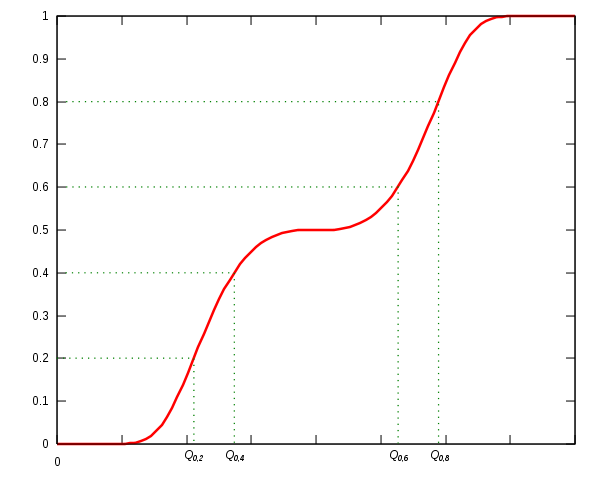
\includegraphics[scale=0.5]{Obrazky/600px-Quantile.png}
\caption{Obrázek z wiki :D, x-ová osa: kvantily, y-ová osa: hodnoty pravděpodobnosti}
\end{center}
\end{figure}
V následujícím zavedeme pojem kvantilu. Kvantil je míra polohy popisující body, ve kterých distribuční funkce náhodné veličiny prochází danou hodnotou, tedy např.: kvantil $F^{-1}(0.5)$ dává hodnotu z definičního oboru distribuční funkce $F$, ve které poprvé nabyde hodnoty $0.5$.
\begin{definition}
Nechť $F$ je distribuční funkce. Zaveďmě funkci $F^{-1}$ předpisem
\begin{equation}
F^{-1}(u) = \inf\lbrace x : F(x) \geq u \rbrace, \enskip 0 < u < 1.
\end{equation}
Pak se funkci $F^{-1}$ nazývá kvantilová funkce odpovídající distribuční funkci $F$, hodnotám $F^{-1}(u)$ se říká kvantily.
\end{definition}

\begin{remark}
Je li $F$ striktně rostoucí, potom je $F^{-1}$ inverzní funkce k $F$.
\end{remark}

\begin{remark}
$Q_{0.5} = F^{-1}(0.5)$ se nazývá medián. Kvantily $Q_{0.25} = F^{-1}(0.25)$, $Q_{0.75} = F^{-1}(0.75)$ se nazývají dolní a horní kvartil.
\end{remark}
\subsection{Charakteristická funkce}
\begin{definition}
Charakteristickou funkci $\psi(t)$ náhodné veličiny $X$ definujeme vzorcem
\begin{equation}
\psi(t) = \mathbf{E}e^{itX} = \mathbf{E}\cos(tX) + i\mathbf{E}\sin(tX), \enskip t \in \mathbb{R}.
\end{equation}
\end{definition}

\begin{remark}
Má-li náhodná veličina $X$ distribuční funkci $F$, pak můžeme psát $\psi(t) = \int e^{itx}dF(x)$ (viz Větu o přenosu integrace v Andělovi). Platí, že $\psi$ je stejnoměrně spojitá, $\psi(0) = 1$ a $|\psi(t)| \leq 1$.
\end{remark}

Charakteristickou funkci lze využít k výpočtu obecných momentů, pokud existují.
\begin{theorem}
Existují-li konečné momenty $\mu_{1}', ..., \mu_{n}',$ pak charakteristická funkce $\psi$ má prvních $n$ derivací a platí
\begin{equation}
\psi^{(k)}(0) = i^{k}\mu_{k}' \enskip k = 1, ..., n, \enskip \psi(t) = \sum_{k = 0}^{n}\mu_{k}' \frac{(it)^{k}}{k!} + O(t^{n}), \enskip t \longrightarrow 0.
\end{equation}
\end{theorem}
\begin{proof}
Viz Rényi (1972).
\end{proof}

Pro zajímavost uveďme následující tvrzení popisující závislost charakteristické funkce a distribuční funkce n. v. $X$.
\begin{theorem}
Nechť $\psi$ je charakteristická finkce odpovídající distribuční funkci $F$ a nechť $a, b (a < b)$ jsou body spojitosti funkce $F$. Pak platí
\begin{equation}
F(b) - F(a)  = \frac{1}{2\pi} \int_{-\infty}^{\infty}\bigg[ \psi(t) \frac{e^{-ita}-e^{-itb}}{2it} - \psi(-t)\frac{e^{ita}-e^{itb}}{2it} \bigg] dt.
\end{equation}
\end{theorem}
\begin{proof}
Viz Renyi (1972).
\end{proof}
Odtud plyne, že distribuční funkce je charakteristickou funkcí jednoznačně určena.

%Uvažujme posloupnost distribučních funkcí $\lbrace F_{n} \rbrace$ a distribuční funkci $F$. Jestliže $F_{n}(x) \longrightarrow F(x)$ v každém bodě $x$, který he bodem spojitosti funkce $F$, pak říkáme, že posloupnost $\lbrace F_{n} \rbrace$ slabě konverguje k $F$. Jestliže distribuční funkce náhodných veličin $\lbrace X_{n} \rbrace$ slabě konvergují k distribuční funkci veličiny $X$, pak píšeme $\mathcal{L}(X_{n}) \longrightarrow \mathcal{X}, nebo také $X_{n} \longrightarrow^{d} X $a říkáme, že veličiny $X_{n}$ konvergují v distribuci k $X$.
\subsection{Základní diskrétní rozdělení pravděpodobnosti}
Uveďme příklady diskrétních rozdělení pravděpodobnosti, v poznámkách bude uveden jejich praktický význam, druh pokusu který modelují, atp.
\begin{definition}{\textbf{(Binomické rozdělení}}
Buď $n$ přirozené číslo a $p \in (0, 1)$. Předpokládejme, že $X$ nabývá pouze hodnot $0, 1, ..., n$ a to s pravděpodobnostmi
\begin{equation}
\textbf{P}(X = k) = \binom{n}{k}p^{k}(1-p)^{n-k}, \enskip k = 0, 1, ..., n.
\end{equation}
Pak říkáme, že $X$ má binomické rozdělení a píšeme $X \sim Bi(n,p)$.
\end{definition}
\begin{proposition}
Nechť  $X \sim Bi(n,p)$. potom $\mathbf{E}X = np$, $\mathbf{var}X = np(1-p)$ a $\psi(t) = (1-p + pe^{it})^{n}$.
\end{proposition}
\begin{proof}
Důkaz se mi nechce dělat, ukáže se to tak, že se nějakými manipulacemi s nekonečnou řadou vyjadřující střední hodnotu získá její součet, rozptyl podobně. Char fce. z definice
\end{proof}

\begin{remark}
Binomické rozdělení je diskrétní rozdělení pravděpodobnosti počtu úspěšných pokusů v posloupnosti $n$ nezávislých pokusů.
Modeluje počet úspěchů ve výběru velikosti $n$ z populace o velikosti $N$ s vracením. Př.: Mám osudí s bílými a černými míčky $n$-krát vytáhnu z osudí míček, poznamenám si barvu a vrátím ho zpět, bin. rozd. udává pravděpodobnost že $k$ míčků bude černých (resp. bílých). Pro $n = 1$ se jedná o tzv alternativní rozdělení.
\end{remark}

\begin{definition}{\textbf{(Hypergeometrické rozdělení)}}
Nechť $N, A$ a $n$ jsou přirozená čísla, přičemž $A < N, n < N$. Nechť $X$ nabývá pouze celočíselných hodnot s pravděpodobnostmi 
\begin{equation}
\textbf{P}(X = x)= \frac{\binom{A}{k}\binom{N-A}{n-k}}{\binom{N}{n}} \enskip pro \enskip \max(0, A + n -N)\leq k \leq \min(A, n).
\end{equation}
Pak říkáme, že $X$ má hypergeometrické rozdělení a píšeme $X \sim Hg(N,A,n)$.
\end{definition}
\begin{proposition}
Nechť $X$ má hypergeometrické rozdělení s parametry $N, A$ a $n$, přičemž $A < N, n < N$.  Je-li $N > 1,$ pak 
\begin{equation}
\mathbf{E}X = \frac{nA}{N}, \enskip \mathbf{var}X = \frac{nA(N-A)}{N^{2}}\bigg( 1 - \frac{n-1}{N-1}\bigg).
\end{equation}
\end{proposition}
\begin{proof}
Důkaz je ponechán pro zvídavého čtenáře, jenž je laskavě odkázán, na literaturu zabývající se pravděpodobností a statistikou.
\end{proof}

\begin{remark}
Poznamenejme, že hypergeometrické rozdělení modeluje pravděpodobnost počtu úspěchů ve výběru velikosti $n$ z populace o velikosti $N$ za předpokladu, že výběr probíhá bez opakování. V případě osudí s míčky z příkladu u binomického rozdělení bychom míčky po vytažení již nevraceli zpět.
\end{remark}

\begin{definition}{\textbf{(Poissonovo rozdělení)}}
Nechť $X$ nabývá pouze hodnot $0, 1, ..., $ a to s pravděpodobnostmi 
\begin{equation}
\textbf{P}(X = k) = \frac{\lambda^{k}}{k!}e^{-\lambda},\enskip k = 0, 1, ...,
\end{equation}
kde $\lambda >0$ je dané číslo. Pak říkáme, že $X$ má Poissonovo rozdělení s parametrem $\lambda$ a píšeme $X \sim Po(\lambda)$.
\end{definition}

\begin{proposition}
Nechť $X \sim Po(\lambda)$. Potom $\mathbf{E}X = \lambda,$ $\mathbf{var}X = \lambda$ a $\psi(t) = e^{\lambda(e^{it}-1)}$.
\end{proposition}
\begin{proof}
Důkaz prvních dvou je z definice manipulací s nekonečnými řadami pro získání jejich součtu, třetí z definice char. fce. Toto mám dokonce naTeXované, ale dávat to sem nebudu, anžto je to delší. Kdyby to někoho hrozně strašně moc zajímalo, nechť se zeptá.
\end{proof}
\begin{remark}
Popisuje pravděpodobnost nastání daného počtu nezávislých jevů v určitém časovém intervalu. Například pravděpodobnost obdržení určitého počtu spamových emailů za týden, za předpokladu, že každý email je na všech ostatních nezávislý.
\end{remark}

\subsection{Spojitá rozdělení pravděpodobnosti}
\begin{definition}{\textbf{(Normální rozdělení)}}
Nechť $ \mu \in \mathbb{R}$ a $\sigma > 0$ jsou dané konstanty (parametry). Normální rozdělení je určeno hustotou
\begin{equation}
f(x) = \frac{1}{\sqrt{2\pi}\sigma}\exp \bigg[ -\frac{(x - \mu)^{2}}{2\sigma^{2}} \bigg]
\end{equation}
a označuje se symbolem $N(\mu, \sigma^{2}).$ V případě, že $\mu = 0$ a $\sigma = 1$ nazýváme $N(0, 1)$ standardní normální rozdělení, jeho hustotu značíme $\phi$ a příslušnou distribuční funkci $\Phi$, máme tedy
\begin{equation}
\phi(x) = \frac{1}{\sqrt{2\pi}}e^{\frac{-x^{2}}{2}}, \enskip \Phi(x) = \int_{-\infty}^{x}\phi(t)dt.
\end{equation}
\end{definition}

\begin{proposition}
Nechť $X \sim N(\mu, \sigma^{2})$ potom $\mathbf{E}X = \mu$, $\mathbf{var}X = \sigma^{2}$, šikmost $\alpha_{3} = 0$ a špičatost $\alpha_{4} = 3$. Charakteristická funkce normálního rozdělení má tvar 
\begin{equation}
\psi(t) = \exp\bigg[ i\mu t - \frac{1}{2}\sigma^{2}t^{2} \bigg].
\end{equation}
\end{proposition}
\begin{proof}
Přímým výpočtem.
\end{proof}

\begin{remark}
Normální rozdělení má v matematické statistice a stochastické analýze veliký význam, mnoho statistických modelů je založeno na předpokladu normálního rozdělení. Příkladem je třeba regrese, kde se předpokládá normální rozdělení závisle proměnných, aby bylo možné odvodit intervaly spolehlivosti, nebo testy vycházející z regresní analýzy, např. analýza rozptylu. V této souvislosti připomeňme také centrální limitní větu, která říká, že průměry z výběrů z nezávislých rozdělení konvergují v distribuci k normálnímu rozdělení.
\end{remark}

\begin{definition}{\textbf{(Weibullovo rozdělení)}}
Nechť $c > 0, \enskip p > 0$. Weibullovi rozdělení $W(c, p)$ má hustotu
\begin{equation}
f(x) = cpx^{p-1}\exp[-cx^{p}], \enskip x > 0.
\end{equation}
Pro volbu $p = 1$ získáme exponenciální rozdělení.
\end{definition}

\begin{proposition}
Nechť $X \sim W(c, p)$, platí
\begin{equation}
\mathbf{E}X = \Gamma\bigg( \frac{p + 1}{p} \bigg) c^{-1/p}, \enskip \mathbf{var}X = \bigg[ \Gamma \bigg( \frac{p+2}{p}\bigg) - \Gamma^{2} \bigg( \frac{p + 1}{p}\bigg) \bigg] c^{-2/p}, 
\end{equation}
kde $\Gamma$ je gamma funkce definovaná pro $a>0$ předpisem $\Gamma(a) = \int_{0}^{\infty} x^{a - 1}e^{-x}dx.$
\end{proposition}

\begin{remark}
Weibullovo rozdělení se využívá ve spolehlivosti při modelování životnosti. Dobře vystihuje dobu do poruchy stárnoucího objektu.
\end{remark}

\section{Náhodný vektor}
\subsection{Definice}
Pro zavedení teorie týkající se náhodných vektorů využijeme poznatků a intuice popsané již při zavádění náhodných veličin.
\begin{definition}{\textbf{(Náhodný vektor)}}
Nechť náhodné veličiny $X_{1}, ..., X_{n}$ jsou definovány na témž pravděpodobnostním prostoru $(\Omega, \mathcal{A}, \textbf{P})$. Pak vektor $\textbf{X} = (X_{1}, ..., X_{n})^{T}$ nazveme náhodným vektorem. 
\end{definition}
\begin{theorem}
Náhodný vektor $\textbf{X}$ je měřitelné zobrazení z pravděpodobnostního prostoru $(\Omega, \mathcal{A}, \textbf{P})$ do $(\mathbb{R}_{n}, \mathcal{B}_{n})$.
\end{theorem}
\begin{proof}
Viz Anděl.
\end{proof}
\subsection{Simultální distribuční funkce, diskrétní a spojitý n. v.}
\begin{definition}{\textbf{(Sdružená (simultální) distribuční funkce)}}
Sdruženou distribučná funkci náhodných veličin $X_{1}, ..., X_{n}$ definovaných na témže pravděpodobnostním prostoru $(\Omega, \mathcal{A}, \textbf{P})$ definujeme vzorcem
\begin{equation}
F(x_{1}, ..., x_{n}) = \textbf{P}(X_{1} < x_{1}, ..., X_{n} < x_{n}).
\end{equation}
\end{definition}

Distribuční funkci odpovídá míra $\textbf{P}_{\textbf{X}}$ indukovaná na $(\mathbb{R}_{n}, \mathcal{B}_{n})$ zobrazením $\textbf{X}$, kterou nazýváme sdružené rozdělení veličin $X_{1}, ..., X_{n}$ (viz definici rozdělení).

Existuje-li taková měřitelná funkce $f$, že platí 
\begin{equation}
F(x_{1}, ..., x_{n}) = \int_{-\infty}^{x_{1}}...\int_{-\infty}^{x_{n}} f(u_{1}, ..., u_{n})du_{1}...du_{n},
\end{equation}
říkáme funkci $f$ sdružená (simultální) hustota. Existuje-li hustota, má $F$ skoro všude derivaci a platí
\begin{equation}
\frac{\partial^{n}F(x_{1}, ..., x_{n})}{\partial x_{1}...\partial x_{n}} = f(x_{1}, ..., x_{n}), \enskip s. v.,
\end{equation}
náhodný vektor $X$ potom nazýváme \textbf{spojitý}.

$\textbf{X}$ nazýváme \textbf{diskrétní} náhodný vektor právě tehdy, když existuje nejvýše spočetná množina $M \subset \mathbb{R}^{n}, \enskip M = M_{1} \times ... \times M_{n}$ taková, že $\textbf{P}(\textbf{X} \in M) = 1$.

Opět můžeme definovat pravděpodobností funkci jako
\begin{equation}
p(\textbf{x}) = \textbf{P}(\textbf{X} = \textbf{x}) = \textbf{P}(X_{1} = x_{1}, ..., X_{n} = x_{n} )
\end{equation}
\subsection{Marginální a podmíněné rozdělení}
\begin{definition}{\textbf{(Marginální rozdělení)}}
Nechť $k_{1}, ..., k_{r}$ jsou různá celá čísla taková, že $1 \leq k_{i} \leq n$ pro $i = 1, ..., r$, přičemž $1 \leq r < n.$ Rozdělení náhodného vektoru $(X_{k_{1}}, ..., X_{k_{r}})^{T}$ se nazývá marginální. 
\end{definition}
\begin{example}{\textbf{(Marginální distribuční funkce)}}
Nechť $\textbf{X} = (X_{1}, ..., X_{n})$ je náhodný vektor. Marginální distribuční funkce $G$ veličin $X_{1}, ... X_{k}$, pro $1 \leq k < n$ je dána vzorcem
\begin{equation}
G(x_{1}, ..., x_{k}) = \lim_{\substack{x_{k+1} \longrightarrow \infty \\ ... \\ x_{n} \longrightarrow \infty}} F(x_{1}, ..., x_{k}, x_{k + 1}, ..., x_{n}).
\end{equation}
\end{example}

\begin{remark}
Existuje-li sdružená hustota, pak existují i marginální hustoty, obrácené tvrzení však neplatí.
\end{remark}

Při popisu podmíněného rozdělení se omezíme jen na uvedení vzorců  pro podmíněnou pravděpodobnostní funkci a hustotu diskrétní nebo spojité náhodné veličiny $X$ za podmínky $Y = y$. Obecně to však není tak jednoduché.


Nechť $p(x,y)$ je simultální pravděpodobnostní funkce diskrétního náhodného vektoru $\textbf{Z} = (X, Y)^{T}$ Pro pravděpodobnostní funkci n.v. $X$ za podmínky $Y = y$ máme 
\begin{equation}
p(x|y) = \frac{p(x,y)}{p(y)}, \enskip pokud \enskip p(y) \neq 0
\end{equation}
kde $p(y)$ je příslušná marginální pravděpodobnstní funkce.

Nechť $f(x,y)$ je sdružená hustota spojitého náhodného vektoru vektoru $\textbf{Z} = (X, Y)^{T}$ Pro hustotu n.v. $X$ za podmínky $Y = y$ máme 
\begin{equation}
f(x|y) = \frac{f(x,y)}{f(y)}, \enskip pokud \enskip f(y) \neq 0
\end{equation}
kde $f(y)$ je příslušná marginální hustota.

\subsection{Nezávislost}
\begin{definition}{\textbf{(Nezávislé náhodné veličiny)}}
Náhodné veličiny $X_{1}, ..., X_{n}$ se nazývají nezávislé, platí-li pro libovolné borelovské množiny vztah
\begin{equation}
\textbf{P}[\cap_{k=1}^{n}\lbrace \omega : X_{k}(\omega) \in B_{k}\rbrace] = \prod_{k = 1}^{n} \textbf{P}\lbrace \omega : X_{k}(\omega) \in B_{k} \rbrace.
\end{equation}
\end{definition}

Z definice je nezávislost náhodných veličin ověřit, uveďme proto formou vět následující kritéria.
\begin{theorem}\label{Kriterium1}
Nechť $\textbf{X}$ má sdruženou distribuční funkci $F$ a nechť $F_{i}$ je marginální distribuční funkce veličiny $X_{i}$, $i = 1, ..., n$. Pak $X_{1}, ..., X_{n}$ jsou nezávislé právě tehdy, když platí $F(x_{1}, ..., x_{n}) = F_{1}(x_{1})\cdot ... \cdot F_{n}(x_{n})$ pro všechna $x_{1}, ..., x_{n}$.
\end{theorem}
\begin{proof}
Viz Renyi (1972).
\end{proof}

Borelovsky měřitelná funkce náhodné veličiny je opět náhodná veličina, funkce nezávislých náhodných veličin jsou také nezávislé. Pro spojité náhodné veličiny máme potom jako důsledek předchozí věty nádlesující tvrzení.
\begin{theorem}
Nechť náhodné veličiny $X_{1}, ..., X_{n}$ mají sdruženou hustotu $f$ a marginální hustoty $f_{1}, ..., f_{n}$. Pak $X_{1}, ..., X_{n}$ jsou nezávislé tehdy a jen tehdy, platí-li
\begin{equation}
f(x_{1}, ..., x_{n}) = f_{1}(x_{1})\cdot ... \cdot f_{n}(x_{n}) \enskip s. \enskip v.
\end{equation}
\end{theorem}
\begin{proof}
Tvrzení je důsledkem Věty \ref{Kriterium1}.
\end{proof}

Pro diskrétní náhodné veličiny máme potom jako důsledek předchozí věty následující tvrzení.
\begin{theorem}
Nechť $X_{1}, ..., X_{n}$ jsou veličiny s diskrétním rozdělením pravděpodobnosti $\mathcal{L}(M_{i}, p_{i})$, mají sdruženou pravděpodobnostní funkci $p$ a marginální pravděpodobnostní funkce $p_{1}, ..., p_{n}$. Pak $X_{1}, ..., X_{n}$ jsou nezávislé tehdy a jen tehdy, platí-li
\begin{equation}
p(x_{1}, ..., x_{n}) = p_{1}(x_{1})\cdot ... \cdot p_{n}(x_{n}) \enskip s. \enskip v.
\end{equation}
\end{theorem}
\begin{proof}
Tvrzení je důsledkem Věty \ref{Kriterium1}.
\end{proof}

\begin{theorem}\label{VetaSeStrHod}
Nechť $X_{1}, ..., X_{n} \in \mathcal{L}^{1}(\Omega)$, pak platí $X_{1}, ..., X_{n}$ jsou nezávislé právě tehdy, když
\begin{equation}
\mathbf{E}(X_{1}, ..., X_{n}) = (\mathbf{E}X_{1}) \cdot ... \cdot (\mathbf{E}X_{n}) 
\end{equation}
\end{theorem}
\begin{proof}
\begin{align*}
\mathbf{E}(X_{1}, ..., X_{n})&= \int ... \int x_{1}...x_{n}dF(x_{1}, ..., x_{n}) \\
&= \int ... \int x_{1}...x_{n}dF(x_{1})...dF(x_{n}) \\
&= \bigg[ \int x_{1}dF(x_{1}) \bigg]...\bigg[ \int x_{n}dF(x_{n}) \bigg]\\ 
&= (\mathbf{E}X_{1})  ... (\mathbf{E}X_{n}),
\end{align*}
kde druhá rovnost je důsledkem Věty \ref{Kriterium1} a třetí je vlastnost L-S integrálu.
\end{proof}

\begin{remark}
Podobná tvrzení lze odovodit pro střední hodnoty a charakteristické funkce.
\end{remark}

\subsection{Číselné charakteristiky}
\begin{definition}{\textbf{(Střední hodnota náhodného vektoru)}}
Nechť $\textbf{X} = (X_{1}, ..., X_{n})^{T}$ je náhodný vektor. Jsou-li náhodné veličiny $X_{i}$, $i = 1, ..., n$ integrovatelné potom definujeme střední hodnotu vektoru $\textbf{X}$ jako
\begin{equation}
\mathbf{E}\textbf{X} = (\mathbf{E}X_{1}, ..., \mathbf{E}X_{n})^{T}.
\end{equation}
\end{definition}

Analogicky se definuje i střední hodnota matice, jejímiž vstupy jsou náhodné veličiny.

\begin{definition}{\textbf{(Kovariance náhodného vektoru)}}
Nechť $\textbf{X} = (X_{1}, ..., X_{n})^{T}$ je náhodný vektor. Jsou-li náhodné veličiny $X_{i}$, $i = 1, ..., n$, kvadraticky integrovatelné, t.j. $\mathbf{E}X_{i} < \infty$ pro $i = 1, ..., n$ pak definujeme kovarianci $\mathbf{cov}(X_{i}, X_{j})$ vztahem
\begin{equation}
\mathbf{cov}(X_{i}, X_{j}) = \mathbf{E}[(X_{i} - \mathbf{E}X_{i})(X_{j} - \mathbf{E}X_{j})] 
\end{equation}
\end{definition}

\begin{proposition}
Nechť $\textbf{X} = (X_{1}, ..., X_{n})^{T}$ je náhodný vektor. Jsou-li náhodné veličiny $X_{i}$, $i = 1, ..., n$, kvadraticky integrovatelné, potom pro kovarianci $X_{i}, X_{j}$ platí
\begin{equation}
\mathbf{cov}(X_{i}, X_{j}) = \mathbf{E}X_{i}X_{j} - \mathbf{E}X_{i}\mathbf{E}X_{j}
\end{equation}
\end{proposition}
\begin{proof}
Zřejmé.
\end{proof}

\begin{proposition}\label{Cauchy-SchwProp}
Nechť $\textbf{X} = (X_{1}, ..., X_{n})^{T}$ je náhodný vektor. Jsou-li náhodné veličiny $X_{i}$, $i = 1, ..., n$, kvadraticky integrovatelné, potom pro kovarianci $X_{i}, X_{j}$ platí
\begin{equation}\label{Cauchy-Schw}
|\mathbf{cov}(X_{i}, X_{j})| \leq \mathbf{var}X_{i} \mathbf{var}X_{j}
\end{equation}
\end{proposition}
\begin{proof}
Nerovnost \eqref{Cauchy-Schw} je přímo Cauchy Schwartzova nerovnost.
\end{proof}

\begin{definition}{\textbf{(Varianční matice)}}
Nechť $\textbf{X} = (X_{1}, ..., X_{n})^{T}$ je náhodný vektor. Jsou-li náhodné veličiny $X_{i}$, $i = 1, ..., n$, kvadraticky integrovatelné, potom matici $\mathbf{var}\textbf{X} = (\mathbf{cov}(X_{i}, X_{j}))_{ij}$ typu $n \times n$ nazýváme varianční maticí vektoru $\textbf{X}$.
\end{definition}

\begin{proposition}\label{Tvrzeni01}
Pro varianční matici $\mathbf{var}\textbf{X} = (\mathbf{cov}(X_{i}, X_{j}))_{ij}$ náhodného vektoru $\textbf{X}$ platí
\begin{equation}
\mathbf{var}\textbf{X} = \mathbf{E}(\textbf{X} - \mathbf{E}\textbf{X})(\textbf{X} - \mathbf{E}\textbf{X})^{T} = \mathbf{E}\textbf{X}\textbf{X}^{T} - (\mathbf{E}\textbf{X})(\mathbf{E}\textbf{X})^{T}.
\end{equation}
\end{proposition}
\begin{proof}
Přímým výpočtem.
\end{proof}

\begin{proposition}{\textbf{(Vlastnosti)}}
Nechť $\textbf{X} = (X_{1}, ..., X_{n})^{T}$ je náhodný vektor, $\textbf{a}$ vektor o $m$ složkách a $\textbf{B}_{m \times n}$ matice typu $m \times n$. Jsou-li náhodné veličiny $X_{i}$, $i = 1, ..., n$ integrovatelné, potom
\begin{equation}
\mathbf{E}(\textbf{a} + \textbf{B}\textbf{X}) = \textbf{a}+ \textbf{B}\mathbf{E}\textbf{X}.
\end{equation}
Jsou-li navíc náhodné veličiny $X_{i}$, $i = 1, ..., n$ kvadraticky integrovatelné, platí
\begin{equation}
\mathbf{var}(\textbf{a} + \textbf{B}\textbf{X}) = \textbf{B}\mathbf{var}\textbf{X}\textbf{B}^{T}.
\end{equation}
\end{proposition}
\begin{proof}
První rovnost plyne z linearity střední hodnoty. V druhé rovnosti se využívá rovnosti první. Máme
\begin{align*}
\mathbf{var}(\textbf{a} + \textbf{B}\textbf{X}) &= \mathbf{E}(\textbf{a} + \textbf{B}\textbf{X})(\textbf{a} + \textbf{B}\textbf{X})^{T} - [\mathbf{E}(\textbf{a} + \textbf{B}\textbf{X})][\mathbf{E}(\textbf{a} + \textbf{B}\textbf{X})]^{T} \\
&=\mathbf{E}[ \textbf{a}\textbf{a}^{T} + \textbf{a}(\textbf{B}\textbf{X})^{T} + \textbf{B}\textbf{X}\textbf{a}^{T} + \textbf{B}\textbf{X}(\textbf{B}\textbf{X})^{T}] \\
&- \textbf{a}\textbf{a}^{T} - \textbf{a}(\mathbf{E}\textbf{X})^{T} \textbf{B}^{T}- \textbf{B}\mathbf{E}\textbf{X}\textbf{a}^{T} - \textbf{B}\mathbf{E}\textbf{X}(\mathbf{E}\textbf{X})^{T}\textbf{B}^{T} \\
&= \textbf{B}\mathbf{E}\textbf{X}\textbf{X}^{T}\textbf{B}^{T} - \textbf{B}\mathbf{E}\textbf{X}(\mathbf{E}\textbf{X})^{T}\textbf{B}^{T} \\
&= \textbf{B}\mathbf{var}\textbf{X}\textbf{B}^{T},
\end{align*}
kde poslední rovnost plyne z Tvrzení \ref{Tvrzeni01}.
\end{proof}

Když uvažujeme dva náhodné vektory $X, Y$ potom můžeme spočítat kovariance složek obou uvažovaných vektorů navzájem a získat tak Kovarianční matici.
\begin{definition}{\textbf{(Kovarianční matice)}}
Nechť vstupy $\textbf{X} = (X_{1}, ..., X_{n})$ a $\textbf{Y} = (Y_{1}, ..., Y_{n})$ jsou kvadraticky integrovatelné, potom definujeme kovarianční matici $\textbf{cov}(\textbf{X}, \textbf{Y})$ vektorů $\textbf{X}$ a $\textbf{Y}$ vzorcem
\begin{equation}
\mathbf{cov}(\textbf{X}, \textbf{Y}) = \mathbf{E}(\textbf{X}- \mathbf{E}\textbf{X})(\textbf{Y}- \mathbf{E}\textbf{Y}).
\end{equation}
\end{definition}

\begin{remark}
Lze ukázat, že 
\begin{equation}
\mathbf{cov}[\textbf{a}_{p \times 1} + \textbf{B}_{p \times n}\textbf{X}, \textbf{c}_{q \times 1} + \textbf{D}_{q \times m}\textbf{Y}] = \textbf{B}[\mathbf{cov}(\textbf{X}, \textbf{Y})]\textbf{D}^{T}.
\end{equation}
Zřejmě pokud $\textbf{Y} = \textbf{X}$ kovarianční matice přechází na varianční matici.
\end{remark}

\begin{proposition}
Jsou-li $X, Y$ nezávislé kvadraticky integrovatelné náhodné veličiny, pak $\mathbf{cov}(X, Y) = 0$. 
\end{proposition}
\begin{proof}
Důkaz je důsledkem Věty \ref{VetaSeStrHod}.
\end{proof}
Veličiny jejichž kovariance je rovna nule se nazývají nekorelované. Náhodné vektory jsou nekorelované, jestliže je jejich kovarianční matice nulová. Nekorelovanost je nutnou, avšak nikoliv postačující podmínkou nezávislosti.

Zaveďme nyní závislost dvou náhodných veličin na sobě.
\begin{definition}
Nechť $X, Y \in \mathcal{L}^{2}(\Omega)$ jsou náhodné veličiny s kladnými rozptyly. Definujeme korelační koeficient pomocí vzorce
\begin{equation}
\rho =  \frac{\mathbf{cov}(X,Y)}{(\sqrt{\mathbf{var}X) (\mathbf{var}Y)}}.
\end{equation}
\end{definition}

\begin{proposition}
Nechť $X, Y \in \mathcal{L}^{2}(\Omega)$ jsou náhodné veličiny s kladnými rozptyly. Pak platí
\begin{itemize}
\item[(i)] $\rho(X, X) = 1$,
\item[(ii)] Nechť $a, b, c, d \in \mathbb{R}$ potom $\rho(a + bX, c + dX) = \textup{sgn}(bd)\rho(X, Y)$,
\item[(iii)] Jestliže jsou $X, Y$ nezávislé, potom $\rho(X, Y) = 0$.
\end{itemize}
\end{proposition}
\begin{proof}
Se mi nechce dělat, všechno plyne z vlastností kovariance.
\end{proof}
\begin{remark}
Z Cauchy Schwartzovy nerovnosti (viz Tvrzení \ref{Cauchy-SchwProp}) plyne, že $-1 \leq \rho \leq 1$.
\end{remark}

\subsection{Transformace náhodného vektoru}
Budeme se nyní zabývat pouze hustotami vzhledem k Lebesgueově míře. Mějme náhodný vektor $\textbf{X}$ s simultální hustotou $\textbf{f}$ a položme $\textbf{Y} = g(\textbf{X})$, kde $g$ je měřitelná funkce. Úlohou je vypočítat sdruženou hustotu vektoru $\textbf{Y}$.

Připomeňme několik pojmů. Zobrazení $\mathbf{f}$ množiny $A$ do množiny $B$ nazveme prostým, platí-li
\begin{equation}
\textbf{x}_{1} \in A, \textbf{x}_{2} \in A, \textbf{x}_{1} \neq \textbf{x}_{2} \Longrightarrow \textbf{f}(\textbf{x}_{1}) \neq \textbf{f}(\textbf{x}_{2}).
\end{equation}

Buď $\textbf{f}: \mathbb{R}^{r} \longrightarrow \mathbb{R}^{r}.$ Je-li $\textbf{y} = \textbf{f}(\textbf{x}),$ kde $\textbf{y} = (y_{1}, ..., y_{r})$ a $\textbf{x} = (x_{1}, ..., x_{r})$, položme $y_{i} = f_{i}(x_{1}, ..., x_{r}),$ $i = 1, ..., r$. Říkáme, že zobrazení $\textbf{f}$ je regulární v množine $M \subset \mathbb{R}^{r}$, jestliže platí:
\begin{itemize}
\item[(i)] Množina $M$ je otevřená.
\item[(ii)] Funkce $f_{1}, ..., f_{r}$ mají parciální derivace prvního řádu spojité v $M$.
\item[(iii)] Pro každé $\textbf{x} \in M$ platí $D_{\mathbf{f}}(\textbf{x}) \neq 0$, kde $D_{\mathbf{f}}$ je Jakobián $\mathbf{f}$.
\end{itemize}

\begin{theorem}{\textbf{(O transformaci náhodného vektoru)}}
Nechť náhodný vektor $\textbf{X} = (X_{1}, ..., X_{n})^{T}$ má hustotu $p$ vzhledem k Lebesgueově míře v $\mathbb{R}^{n}$. Nechť $\textbf{g}$ je zobrazení z $\mathbb{R}^{n}$ do $\mathbb{R}^{n}$, které je regulární a prosté na takové otevřené množině $G$, pro niž platí $\int_{G} p(\textbf{x})d\textbf{x} = 1$. Označme $\bm{\tau}$ inverzní zobrazení k $\textbf{g}: G \longrightarrow \textbf{g}(G).$ Pak náhodný vektor $\textbf{Y} = \textbf{g}(\textbf{X})$ má hustotu vzhledem k Lebesgueově míře a tato hustota je rovna
\[
q(\textbf{y}) = 
\begin{cases}{c}
p[\bm{\tau}(\textbf{y})]|D_{\bm{\tau}}(\textbf{y})| & \enskip pro \enskip \textbf{y} \in \textbf{g}(G), \\
0 & \enskip pro \enskip \textbf{y} \notin \textbf{g}(G).
\end{cases}
\]
\end{theorem}
\begin{proof}
Viz Anděl.
\end{proof}
\subsection{Zákony velkých čísel}
Připomeňme nejprve jaké máme typy konvergencí pro náhodné veličiny.
\begin{definition}
Nechť $\lbrace X_{n} \rbrace_{n \in \mathbb{N}}$ je posloupnost náhodných veličin definovaných na pravděpodobnostním prostoru $(\Omega, \mathcal{A}, \textbf{P})$ s hodnotami v $(\mathbb{R}, \mathcal{B})$ a nechť $X$ je náhodná veličina definovaná na pravděpodobnostním prostoru $(\Omega, \mathcal{A}, \textbf{P})$ s hodnotami v $(\mathbb{R}, \mathcal{B})$. Nechť $\lbrace F_{n} \rbrace_{n \in \mathbb{N}}$ je posloupnost příslušných distribučních funkcí $X_{n}$ a $F$ je distribuční funkce $X$.  Řekneme že,
\begin{itemize}
\item[(i)] $X_{n}$ konverguje k $X$ skoro jistě a značíme $X_{n} \xrightarrow{s.j.} X$ jestliže $X_{n}(\omega) \longrightarrow X(\omega)$ pro $\forall \omega \in A$ taková, že $\textbf{P}(A) > 0$,
\item[(ii)] $X_{n}$ konverguje k $X$ v $L^{p}$ a značíme $X_{n} \xrightarrow{L^{p}} X$, jestliže 
\begin{equation}
\mathbf{E}[|X_{n} - X|^{p}]^{1/p} = \bigg[ \int |X_{n}(\omega) - X(\omega)|^{p}d\textbf{P}(\omega)\bigg]^{1/p} \longrightarrow 0,
\end{equation}
\item[(iii)] $X_{n}$ konverguje k $X$ v pravděpodobnosti a značíme $X_{n} \xrightarrow{\mathbf{P}} X$, jestliže $\textbf{P}(|X_{n} - X| > \epsilon) \longrightarrow 0$ pro všechna $\epsilon > 0$.
\item[(iv)] $X_{n}$ konverguje k $X$ v distribuci a značíme $X_{n} \xrightarrow{d} X$, jestliže $F_{n}(x) \longrightarrow F(x)$ v každém $x$, jenž je bodem spojitosti $F$
\end{itemize}
\end{definition}

\begin{remark}
Konvergence skoro jistě implikuje konvergenci v pravděpodobnosti, konvergence v $L^{p}(\Omega)$ implikuje konvergenci v pravděpodobnosti, konvergence v pravděpodobnosti implikuje konvergenci v distribuci.
\end{remark}

\begin{theorem}\label{Chebychev1}{\textbf{(Čebyševova nerovnost)}}
Nechť náhodná veličina $X \in \mathcal{L}^{2}(\Omega)$ má střední hodnotu $\mu$ a rozptyl $\sigma^{2}$. Pak pro každé $\epsilon > 0$ platí
\begin{equation}
\textbf{P}(|X - \mu | \geq \epsilon) \leq \frac{\sigma^{2}}{\epsilon^{2}}
\end{equation}
\end{theorem}

\begin{proof}
Máme
\begin{align*}
\textbf{P}(|X - \mu | \geq \epsilon) &= \int_{|X - \mu | \geq \epsilon} d\textbf{P} \leq \frac{1}{\epsilon^{2}}\int_{|X - \mu | \geq \epsilon} (X - \mu)^{2}d\textbf{P} \\
&\leq \frac{1}{\epsilon^{2}} \int (X - \mu)^{2}d\textbf{P} = \frac{\sigma^{2}}{\epsilon^{2}}.
\end{align*}
\end{proof}

\begin{theorem}{\textbf{(Čebyševova - Slabý zákon velkých čísel)}}
Nechť $X_{1}, X_{2}, ... \in \mathcal{L}^{2}(\Omega)$ jsou nezávislé náhodné veličiny, které mají stejné střední hodnoty $\mu$ a stejne rozptyly $\sigma^{2}$. Označme
\begin{equation}
\hat{X}_{n} = \frac{1}{n}\sum_{i = 1}^{n} X_{i}.
\end{equation}
Jestliže $n \longrightarrow \infty$, pak $\hat{X}_{n} \xrightarrow{\mathbf{P}} \mu$.
\end{theorem}
\begin{proof}
Důsledek Věty \ref{Chebychev1}.
\end{proof}

\begin{theorem}{\textbf{(Chinčinova - Slabý zákon velkých čísel)}}
Nechť $X_{1}, X_{2}, ... \in \mathcal{L}^{1}(\Omega)$ jsou nezávislé náhodné veličiny, které mají stejné rozdělení s konečnou střední hodnotou $\mu$. Jestliže $n \longrightarrow \infty$, pak $\hat{X}_{n} \xrightarrow{\mathbf{P}} \mu$.
\end{theorem}
\begin{proof}
Viz Rényi (1972).
\end{proof}

\begin{theorem}{\textbf{(Kolmogorova - Silný zákon velkých čísel)}}
Nechť $X_{1}, X_{2}, ... \in \mathcal{L}^{1}(\Omega)$ jsou nezávislé náhodné veličiny, které mají stejné rozdělení s konečnou střední hodnotou $\mu$. Jestliže $n \longrightarrow \infty,$ potom $\hat{X}_{n} \xrightarrow{s.j.} \mu$ skoro jistě.
\end{theorem}
\begin{proof}
Viz Rényi (1972).
\end{proof}
Povšimněme si rozdílu, zatímco slabý zákon velkých čísel dává konvergenci v pravděpodobnosti, silný zákon velkých čísel konvergenci skoro jistě.

\subsection{Centrální limitní věty}
Centrální limitní věty popisují konvergenci v distribuci vhodně normovaného součtu náhodných veličin k normálnímu rozdělení.

\begin{theorem}{\textbf{Lindebergova}}
Nechť $X_{1}, X_{2}, ... \in \mathcal{L}^{2}(\Omega) $ jsou nezávislé stejně rozdělené náhodné veličiny se střední hodnotou $\mu$ a rozptylem $\sigma^{2}$. Pak pro $n \longrightarrow \infty$ platí 
\begin{equation}
\frac{X_{1}+ ... + X_{n} - n\mu}{\sqrt{n}} \xrightarrow{d} N(0, \sigma^{2}).
\end{equation}
\end{theorem}
\begin{proof}
Viz Anděl (1985).
\end{proof}

\begin{remark}
Podobná věta existuje i pro náhodné vektory. Tvrzení se liší pouze tím, že jednorozměrné vstupy jsou nahrazeny vektory (viz Anděl)
\end{remark}

\section{Základy statistiky}
náhodný  výběr,  statistiky,  bodové  a  intervalové  odhady parametrů,  nestrannost,  konzistence  a  vydatnost  odhadu, maximálně  věrohodné odhady, odhady metodou momentů, testování hypotéz.

$\Theta$ - parametrický prostor; $\theta$ - jedno nebo více-rozměrný parametr.

\begin{definition}
Nechť $\left(\Omega, \mathcal{A}, P_{\theta} \right)$ je pravděpodobnostní prostor, $X_1,\ldots,X_n$ jsou nezávislé $k-$rozměrné náhodné vektory na $\left(\Omega, \mathcal{A}, P_{\theta} \right)$ s distribuční funkcí $F_{\theta}$ z třídy distribuční funkce $\{F_{\theta}, \theta \in \Theta \}$. Pak  $X_1,\ldots,X_n$ nazýváme \textit{náhodný výběr rozsahu n z k-rozměrného rozdělení s distribuční funkcí $F_{\theta}$}. 
\end{definition}

\begin{definition}
Nechť $X_1,\ldots,X_n$ je náhodný výběr z rozdělení s distribuční funkcí $F_{\theta}$. Libovolnou transformaci náhodného výběru $T=T \left(X_1,\ldots,X_n \right)$ nazýváme \textit{statistika}. 
\end{definition}

\begin{definition}
\textit{Parametrická funkce} je libovolná reálná funkce $\gamma$ parametru $\theta \in \Theta$.
\end{definition}

\begin{definition}
Nechť $X_1,\ldots,X_n$ je náhodný výběr z rozdělení s distribuční funkce $F_{\theta}$. \textit{Bodový odhad} parametrické funkce $\gamma \left(\theta \right)$ je odhad daný statistikou $T=T \left(X_1,\ldots,X_n \right)$, kterým se snažíme v nějakém smyslu aproximovat hodnotu $\gamma \left(\theta \right)$.
\end{definition}

\begin{definition}
Nechť $X_1,\ldots,X_n$ je náhodný výběr z rozdělení s distribuční funkcí $F_{\theta}, \theta \in \Theta$. Pak nazýváme \begin{itemize}
\item $\bar{X}_n = \bar{X} = \frac{1}{n} \sum_{i=1}^{n} X_i$ výběrový průměr
\item $S_{n}^{2} = \frac{1}{n-1}\sum_{i=1}^{n} \left( X_i - \bar{X}\right)^2$ výběrový rozptyl 
\item $S_{n} = \sqrt{S_{n}^{2}}$ výběrová směrodatná odchylka
\item $F_{n}^{*} = \frac{1}{n} \sum_{i=1}^{n} I_{\left( - \infty , x \rangle \right.} \left(X_i \right)$ výběrová (empirická) distribuční funkce kde $I_A \left( x \right) = 1$ pro $x \in A$ a $I_A \left( x \right) = 0$ pro $x \notin A$
\item $M_r = \frac{1}{n} \sum_{i=1}^{n} \left( X_i - \bar{X}\right)^r$ výběrový r-tý centrální moment
\end{itemize}
\end{definition}

\begin{notes}[Střední hodnota a rozptyl výběrového průměru]
$E \left(X_i \right) = \mu$, $D \left(X_i \right) = \sigma^2 $\\
$E \left(\bar{X} \right) = E \left[\frac{1}{n} \sum_{i=1}^{n} X_i \right] = \frac{1}{n} \sum_{i=1}^{n} E\left[ X_i \right] = \mu$\\
$D \left(\bar{X} \right) = D \left[\frac{1}{n} \sum_{i=1}^{n} X_i \right] = \frac{1}{n^2} \sum_{i=1}^{n} D\left[ X_i \right] = \frac{1}{n^2} n \sigma^2 = \frac{\sigma^2}{n}$
\end{notes}

\begin{definition}
Nechť $X_1,\ldots,X_n$ je náhodný výběr z rozdělení s distribuční funkcí $F_{\theta}$. Statistika $T=T \left(X_1,\ldots,X_n \right)$ je \textit{nestranný odhad} parametrické funkce $\gamma \left(\theta \right)$, jestliže pro každé $\theta \in \Theta$ $E_{\theta} \left(T \right) = \gamma \left(\theta \right)$.
\end{definition}

\begin{definition}
Nechť $X_1,\ldots,X_n$ je náhodný výběr z rozdělení s distribuční funkcí $F_{\theta}$. $T=T \left(X_1,\ldots,X_n \right)$ a $T^{*}=T^{*} \left(X_1,\ldots,X_n \right)$ statistiky jsou různé nestrané odhady $\gamma \left(\theta \right)$. Pak řekneme, že statistika $T$ je \textit{vydatnějším odhadem} parametrické funkce $\gamma \left(\theta \right)$ než $T^{*}$, pokud platí $$D \left( T \right) < D \left( T^{*} \right).$$
\end{definition}

\begin{theorem}
Nechť $X_1,\ldots,X_n$ je náhodný výběr z rozdělení se střední hodnotou $\mu \left(\theta \right)$. Pak $\bar{X}$ je nestranný odhad $\mu \left(\theta \right)$.
\end{theorem}

\begin{theorem}
Nechť $X_1,\ldots,X_n$ je náhodný výběr rozsahu $n$ z rozdělení s konečným rozptylem $\sigma^2 \left(\theta \right)$, $\forall \theta \in \Theta $. Pak $S_{n}^{2}$ je nestranný odhad $\sigma^2 \left(\theta \right)$. 
\end{theorem}

\begin{theorem}
Nechť $X_1,\ldots,X_n$ je náhodný výběr z rozdělení s distribuční funkcí $F_{\theta}$. Označme $\mathbb{X} = \left(X_1,\ldots,X_n \right)^T$. Řekneme, že statistika $T=T \left(X_1,\ldots,X_n \right)$ je \textit{nejlepším nestranným lineárním odhadem} parametrické funkce $\gamma \left(\theta \right)$, jestliže je lineární transformací náhodného výběru tvaru $T = \mathbf{a}^T\mathbb{X}$, $\mathbf{a} \in \mathbf{R}^n$, pro její střední hodnotu platí $E_{\theta} \left(T \right) = \gamma \left(\theta \right)$ a 
$$D \left(T\right) \leq D\left(\mathbf{c}^T \mathbb{X} \right)$$ 
pro libovolné $\mathbf{c}^T \in  \mathbb{R}^n$ takové, že $E_{\theta} \left(\mathbf{c}^T \mathbb{X} \right) = \gamma \left(\theta \right)$, $\forall \theta \in \Theta$. 
\end{theorem}

\begin{theorem}
Nechť $X_1,\ldots,X_n$ je náhodný výběr z rozdělení se střední hodnotou $\mu \left(\theta \right)$. Pak $\bar{X}$ je nejlepší nestranný lineární odhad $\mu \left(\theta \right)$.
\end{theorem}

\begin{definition}
Nechť $X_1,\ldots,X_n$ je náhodný výběr rozsahu $n$ z rozdělení s distribuční funkcí $F_{\theta}$. Řekneme, že statistika $T=T \left(X_1,\ldots,X_n \right)$ je \textit{konzistentním odhadem} parametrické funkce $\gamma \left(\theta \right)$, když $$P\{ \lim_{n \to \infty} T \left(X_1,\ldots,X_n \right) = \gamma \left(\theta \right) \}=1, \, \forall \theta \in \Theta.$$
\end{definition}

\begin{definition}
Nechť $X_1,\ldots,X_n$ je náhodný výběr z rozdělení s distribuční funkcí $F_{\theta}$, $\theta \in \Theta$, $ \gamma \left(\theta \right)$ je daná parametrická funkce, $\alpha \in \left(0,1 \right)$, $D=D \left(X_1,\ldots,X_n \right)$, $H=H \left(X_1,\ldots,X_n \right)$ jsou statistiky. Potom $\langle D,H \rangle$ nazýváme $100(1-\alpha)\%$ \textit{interval spolehlivosti} pro parametrickou funkci $\gamma \left(\theta \right)$, právě když $$P\left(D \leq \gamma \left(\theta \right) \leq H \right) = 1-\alpha.$$ Jestliže  $$P\left(D \leq \gamma \left(\theta \right) \right) = 1-\alpha$$ nazýváme statistikou D \textit{dolním odhadem} parametrické funkce $\gamma \left(\theta \right)$ se spolehlivostí $1-\alpha$. Jestliže  $$P\left( \gamma \left(\theta \right) \leq H \right) = 1-\alpha$$ nazýváme statistikou H \textit{horním odhadem} parametrické funkce $\gamma \left(\theta \right)$ se spolehlivostí $1-\alpha$. 
\end{definition}

Náhodné výběry z normálního rozdělení:
\begin{theorem}
Nechť $X_1,\ldots,X_n$ je náhodný výběr rozsahu $n$ z normálního rozdělení $N\left(\mu,\sigma^2 \right)$. Pak \begin{enumerate}
\item $\bar{X} \sim N\left(\mu,\frac{\sigma^2}{n} \right)$
\item Statistika $U = \sqrt{n}\frac{\bar{X}-\mu}{\sigma} \sim N\left(0,1 \right)$
\item Statistika $K = \frac{n-1}{\sigma^2} S_{n}^{2} \sim \chi^2 \left(n-1 \right)$
\item Statistiky $\bar{X}$ a $S_{n}^{2}$ jsou nezávislé
\item Statistika $T = \sqrt{n}\frac{\bar{X}-\mu}{S_n} \sim t\left(n-1 \right)$
\end{enumerate}
\end{theorem}

\begin{dusledek}
Nechť $X_1,\ldots,X_n$ je náhodný výběr rozsahu $n$ z normálního rozdělení $N\left(\mu,\sigma^2 \right)$, kde $\mu$, $\sigma^2$ jsou neznámé parametry, $\alpha \in \left(0,1 \right)$. Pak \begin{enumerate}
\item $\langle \bar{X} - t_{1-\frac{\alpha}{2}} \left(n-1 \right)\frac{S_n}{\sqrt{n}}, \bar{X} + t_{1-\frac{\alpha}{2}} \left(n-1 \right)\frac{S_n}{\sqrt{n}} \rangle$ je $100\left(1-\alpha \right)\%$ interval spolehlivosti pro střední hodnotu $\mu$
\item $\langle \frac{\left(n-1 \right) S_{n}^{2}}{\chi_{1-\frac{\alpha}{2}}^{2} \left(n-1 \right)}, \frac{\left(n-1 \right) S_{n}^{2}}{\chi_{\frac{\alpha}{2}}^{2} \left(n-1 \right)} \rangle$ je $100\left(1-\alpha \right)\%$ interval spolehlivosti pro rozptyl $\sigma^2$
\end{enumerate} 
\end{dusledek}

\begin{theorem}
Nechť $X_1,\ldots,X_n$ je náhodný výběr rozsahu $n_1$ z normálního rozdělení $N\left(\mu_1,\sigma_{1}^{2} \right)$ a $Y_1,\ldots,Y_n$ je náhodný výběr rozsahu $n_2$ z normálního rozdělení $N\left(\mu_2,\sigma_{2}^{2} \right)$. Dále nechť náhodné výběry $X_1,\ldots,X_{n_1}$ a $Y_1,\ldots,Y_{n_2}$ jsou nezávislé. Pak \begin{enumerate}
\item Statistika $U = \frac{\bar{X}-\bar{Y}-\left(\mu_1 - \mu_2 \right)}{\sqrt{ \frac{\sigma_{1}^{2}}{n_1} +  \frac{\sigma_{2}^{2}}{n_2} }} \sim N\left(0,1 \right)$
\item Je-li $\sigma_{1}^{2} = \sigma_{2}^{2}$, pak statistika $T = \frac{\bar{X}-\bar{Y}-\left(\mu_1 - \mu_2 \right)}{S}\sqrt{\frac{n_1 n_2}{n_1 + n_2}} \sim t \left(n_1 + n_2 -2 \right)$,

kde $S^2 = \frac{1}{n_1 +n_2 -2} \left( \left( n_1 - 1 \right) S_{X}^{2} + \left( n_2 - 1 \right) S_{Y}^{2} \right)$
\item Statistika $F = \frac{S_{X}^{2}}{ S_{Y}^{2}} \frac{\sigma_{2}^{2}}{\sigma_{1}^{2}} \sim F\left(n_1 - 1, n_2 -1 \right)$
\end{enumerate}
\end{theorem}

\begin{dusledek}
Nechť $X_1,\ldots,X_n$ je náhodný výběr rozsahu $n_1$ z normálního rozdělení $N\left(\mu_1,\sigma_{1}^{2} \right)$ a $Y_1,\ldots,Y_n$ je náhodný výběr rozsahu $n_2$ z normálního rozdělení $N\left(\mu_2,\sigma_{2}^{2} \right)$. Dále nechť náhodné výběry $X_1,\ldots,X_{n_1}$ a $Y_1,\ldots,Y_{n_2}$ jsou nezávislé. Předpokládejme, že $\mu_1$, $\mu_2$, $\sigma_{1}^{2}$, $\sigma_{2}^{2}$ jsou neznámé parametry, $\alpha \in \left(0,1\right)$. Pak \begin{enumerate}
\item $\langle \bar{X} - \bar{Y} -  t_{1-\frac{\alpha}{2}} \left(n_1 + n_2 -2 \right) S \sqrt{\frac{n_1 + n_2}{n_1 n_2}}, \bar{X} - \bar{Y} +  t_{1-\frac{\alpha}{2}} \left(n_1 + n_2 -2 \right) S \sqrt{\frac{n_1 + n_2}{n_1 n_2}} \rangle$ je $100\left(1-\alpha \right)\%$ interval spolehlivosti pro rozdíl středních hodnot $\mu_1 - \mu_2$ za předpokladu, že $\sigma_{1}^{2} = \sigma_{2}^{2}$
\item $\langle \frac{ S_{X}^{2}/ S_{Y}^{2}}{F_{1-\frac{\alpha}{2}} \left(n_1 -1, n_2 -1 \right)}, \frac{ S_{X}^{2}/ S_{Y}^{2}}{F_{\frac{\alpha}{2}} \left(n_1 -1, n_2 -1 \right)}   \rangle$ je $100\left(1-\alpha \right)\%$ interval spolehlivosti pro podíl rozptylů $\sigma_{1}^{2} / \sigma_{2}^{2}$
\end{enumerate} 
\end{dusledek}

\subsection{Metoda maximální věrohodnosti (Maximum likelihood estimation)} 
Nechť $\mathbf{X}=\left(X_1,\ldots,X_n\right)^T$ je náhodný výběr z rozdělení s hustotou $f\left( x,\pmb{\theta}\right)$, $\pmb{\theta}=\left(\theta_1,\ldots,\theta_r\right)^T \in \pmb{\Theta}$ a $\pmb{\Theta} = \left(a_1, b_1\right)\times \ldots \times \left(a_r, b_r\right)$.

Pro pevnou hodnotu $\mathbf{x}$ nazýváme $$L \left(\pmb{\theta}, \mathbf{x} \right) = f\left(\pmb{\theta}, \mathbf{x} \right) = \prod_{i=1}^{n} f\left(\pmb{\theta},x_i \right) $$ \textit{věrohodnostní funkcí}.

\subsubsection{Maximální věrohodnostní odhad pro 1 parametr}
\begin{itemize}
\item $r=1$
\item $\hat{\theta}$ nazveme \textit{maximálně věrohodnostný odhad parametru $\theta$}, jestliže $$L \left(\hat{\theta}, \mathbf{x} \right) \geq L \left(\theta, \mathbf{x} \right), \forall \theta \in \Theta.$$
\item \textit{Věrohodnostní rovnice} $\frac{\partial L \left(\theta, \mathbf{x} \right)}{\partial \theta} = 0.$
\item \textit{Podmínka maxima} $\frac{\partial^2 L \left(\theta, \mathbf{x} \right)}{\partial \theta^2} < 0.$
\item \textit{Logaritmická věrohodnostní funkce} $$\mathcal{L} = \mathcal{L} \left(\theta, \mathbf{x} \right) = \ln \prod_{i=1}^{n} f\left(\theta,x_i \right) = \sum_{i=1}^{n} \ln f\left(\theta,x_i \right).$$
\end{itemize}

\subsubsection{Maximální věrohodnostní odhad pro vícerozměrný parametr}
\begin{itemize}
\item $r>1$, $\pmb{\theta}=\left(\theta_1,\ldots,\theta_r\right)^T$
\item $\hat{\pmb{\theta}}$ nazveme \textit{maximálně věrohodnostný odhad parametru $\pmb{\theta}$}, jestliže $$L \left(\hat{\pmb{\theta}}, \mathbf{x} \right) \geq L \left(\pmb{\theta}, \mathbf{x} \right), \forall \pmb{\theta} \in \pmb{\Theta}.$$
\item \textit{Věrohodnostní rovnice} $\frac{\partial L \left(\pmb{\theta}, \mathbf{x} \right)}{\partial \theta_j} = 0,\, \forall j=1,\ldots\ r.$
\item \textit{Podmínka maxima} $\frac{\partial^2 L \left(\pmb{\theta}, \mathbf{x} \right)}{\partial \theta_j \partial \theta_k} < 0,\, \forall j,k=1,\ldots\ r.$
\item \textit{Logaritmická věrohodnostní funkce} $$\mathcal{L} = \mathcal{L} \left(\pmb{\theta}, \mathbf{x} \right) = \ln \prod_{i=1}^{n} f\left(\pmb{\theta},x_i \right) = \sum_{i=1}^{n} \ln f\left(\pmb{\theta},x_i \right).$$
\end{itemize}

\subsection{Momentová metoda}
Nechť $\mathbf{X}=\left(X_1,\ldots,X_n\right)^T$ je náhodný výběr z rozdělení s hustotou $f\left( x,\pmb{\theta}\right)$, $\pmb{\theta}=\left(\theta_1,\ldots,\theta_r\right)^T \in \pmb{\Theta}$.
\begin{itemize}
\item Předpokládejme, že pro každé $\pmb{\theta}$ existuje \textit{obecný moment} $$\mu'_k\left(\pmb{\theta}\right) = EX_{i}^{k}, \, k=1,\ldots,r.$$
\item \text{Výběrový moment} $$M'_k = \frac{1}{n} \sum_{i=1}^{n} X_{i}^{k}, \, k=1,2,\ldots$$
\item \text{Momentová metoda} $$\mu'_k\left(\pmb{\theta}\right)  = M'_k , k=1,\ldots,r$$
\item Snadno se vypočítá, ale nebýva vydatná. Používá se především jako počáteční hodnoty do numerických výpočtů metody maximální věrohodnorti a dalších metod.
\end{itemize}

\subsection{Testování hypotéz}
\begin{definition}
Nechť $X_1,\ldots,X_n$ je náhodný výběr z rozdělení s distribuční funkcí $F_{\theta}$, $\theta \in \Theta$ a $ \gamma \left(\theta \right)$ je parametrická funkce. Pak definujeme pojmy \begin{itemize}
\item nulová hypotéza - tvrzení o vlastnostech rozdělení, např. $H_0 : \gamma \left(\theta \right) = \gamma_0$
\item alternativa, např.  $H_1 : \gamma \left(\theta \right) \neq \gamma_0$ (oboustranná),  $H_1 : \gamma \left(\theta \right) > \gamma_0$ (jednostranná)
\item statistický test - pravidlo, které každé realizaci náhodného výběru přiřadí právě jedno ze dvou rozhodnutí: buď "zamítneme $H_0$" nebo "nezamítáme $H_0$"
\item chyba I. druhu - nastává pokud zamítáme $H_0$, když $H_0$ platí
\item chyba II. druhu - nastává pokud nezamítáme $H_0$, když $H_0$ neplatí (tj. platí $H_1$)
\item hladina významnosti testu $\alpha \in \left( 0,1 \right)$ - nejvyšší povolená chyba I. druhu
\item síla testu = $1 -$ pravděpodobnost chyby II. druhu = $1 - \beta$
\item p-hodnota - nejmenší hladina významnosti při které bychom $H_0$ ještě zamítli 
\end{itemize}
\end{definition}

\begin{notes}[Test pomocí intervalu spolehlivosti]
Uvažujeme test $H_0 : \gamma \left(\theta \right) = \gamma_0$ proti $H_1 : \gamma \left(\theta \right) \neq \gamma_0$. Stanovme si hladinu významnosti $\alpha$ (většinou 0,05). Využijeme $\langle D, H \rangle$ $100\left(1-\alpha \right)\%$ interval spolehlivosti pro parametrickou funkci $\gamma \left(\theta \right)$. Při $H_0$ tedy platí $P \left(D \leq \gamma_0 \leq H \right) = 1 - \alpha$. Proto test stanovíme následovně:\begin{itemize}
\item Při $\gamma \left(\theta \right) \in \langle D, H \rangle$ nezamítáme $H_0$ na hladině významnosti $\alpha$
\item Při $\gamma \left(\theta \right) \notin \langle D, H \rangle$ zamítáme $H_0$ na hladině významnosti $\alpha$
\end{itemize}
Pro test $H_0 : \gamma \left(\theta \right) = \gamma_0$ proti $H_1 : \gamma \left(\theta \right) > \gamma_0$ využijeme dolní odhad $D$ a $H_0$ zamítáme pokud $D > \gamma_0$ na hladině významnosti $\alpha$.\\
Pro test $H_0 : \gamma \left(\theta \right) = \gamma_0$ proti $H_1 : \gamma \left(\theta \right) < \gamma_0$ využijeme horní odhad $H$ a $H_0$ zamítáme pokud $\gamma_0 > H$ na hladině významnosti $\alpha$.
\end{notes}

\begin{notes}[Test pomocí testovacího kritéria]
Testové kritérium pro test $H_0 : \gamma \left(\theta \right) = \gamma_0$ je vhodná statistika $T=T \left(X_1,\ldots,X_n \right)$. Obor hodnot je rozdělen na dvě disjunktní množiny: kritický obor $W_{\alpha}$ a jeho doplněk $\bar{W}_{\alpha}$. Pro kritický obor musí platit $P \left(T \in W_{\alpha} \right) \leq \alpha$. Test stanovíme následovně: \begin{itemize}
\item Při $t \in W_{\alpha}$ zamítáme $H_0$ na hladině významnosti $\alpha$
\item Při $t \notin W_{\alpha}$ nezamítáme $H_0$ na hladině významnosti $\alpha$
\end{itemize}
\end{notes}
%\itemize{\textbf{Zdroje:}}
%    \item Anděl, J., Základy matematické statistiky, Praha 2013
%    \item Hübnerová, Z., Studijní materiály pro SP1 a SP3, Brno 2016

\begin{figure}[H]
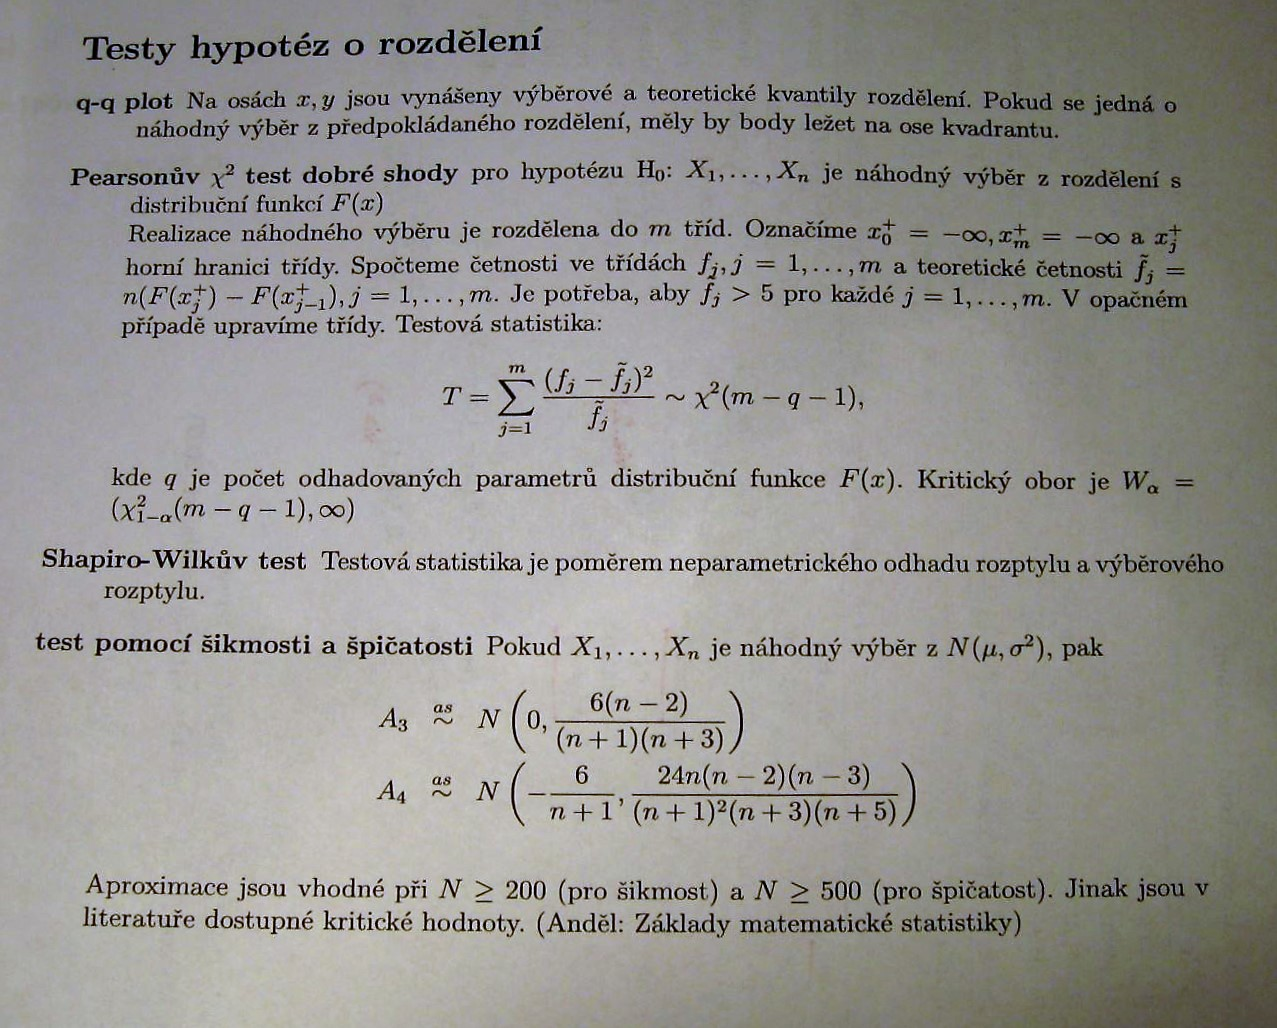
\includegraphics[scale=1]{Obrazky/stat4.png}
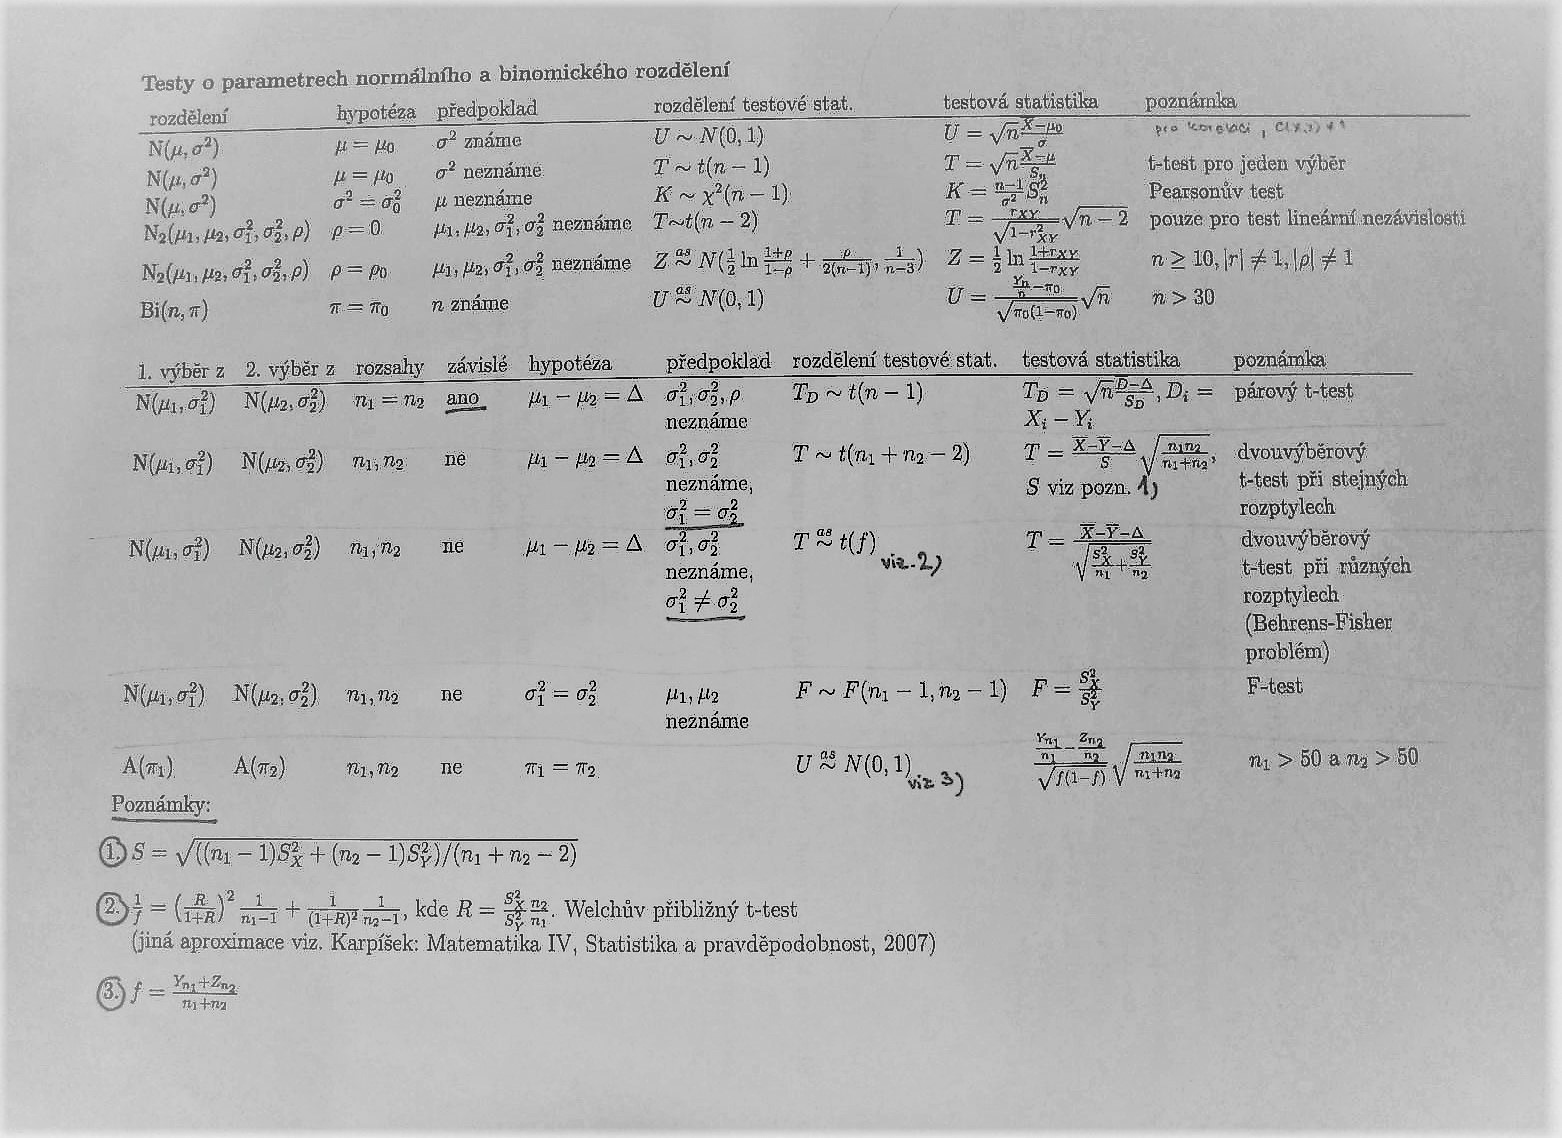
\includegraphics[scale=1]{Obrazky/stat2.png}
\end{figure}

\newpage
\section{Regresní analýza}



lineární regresní model, metoda nejmenších čtverců, bodové a intervalové odhady parametrů, testy hypotéz o regresních koeficientech, regresní diagnostika, nelineární model, korelační analýza.

Toto téma je zpracované na MATEMATIKA Online pro strojaře. Odkaz na stránky s PDF (musí se okopírovat odkaz do nového okna) mathonline.fme.vutbr.cz/Regresni-analyza/sc-1159-sr-1-a-185/default.aspx

\subsection{Lineární regresní model}
Hledání a zkoumání závislosti proměnných, které získáme jako reálná data z experimentu.

\begin{itemize}
    \item $Y, X_1,..., X_k$ náhodné veličiny na $(\Omega, \pmb{\mathcal{A}}, P)$
    \item $X_1,..., X_k$ jsou nezávislé proměnné
    \item $Y$ je závislá proměnná
    \item $\hat{Y} = \beta_1 X_1 + ... + \beta_k X_k$, kde $\beta_1, ..., \beta_k$ jsou neznámé parametry
    \item $E (Y - \hat{Y})^{2}$ je střední kvadratická chyba predikce
    \item Hledáme parametry $\beta_0$ a $\pmb{\beta}$ tak, aby $E (Y - \hat{Y})^{2}$ byla minimální 
    \item vezmeme-li $X_1 = x_1, ..., X_k = x_k$ pak    DOPLNIT, kde $e$ je náhodná chyba
    \item $Y, x_1,..., x_k$ pozorujeme (měříme) $n$ krát
    \item $Y_i, x_{i1},..., x_{ik}$ $i$-té pozorování $Y, x_1,..., x_k$ pro $i=1,2,...,n$
    \item Můžeme tedy napsat soustavu rovnic \begin{align*}
Y_1 &= \beta_1 x_{11} + ... + \beta_k x_{1k} + e_1 \\
    Y_2 &= \beta_1 x_{21} + ... + \beta_k x_{2k} + e_2 \\
    \vdots \\
    Y_n &= \beta_1 x_{n1} + ... + \beta_k x_{nk} + e_n    
\end{align*} 
    Pak $$\mathbf{Y} = \mathbf{X} \pmb{\beta} + \mathbf{e}$$ 
\end{itemize}

\begin{predpoklady}
\itemize
    \item $E\mathbf{e}=\mathbf{0}$
    \item var$\mathbf{e}=\sigma^2 \mathbf{I},$ kde $\sigma^2 > 0$ je neznámý parametr 
\end{predpoklady}

\begin{definition}
Model 
\begin{align*}
\mathbf{Y} &= \mathbf{X} \pmb{\beta} + \mathbf{e} \\
E \mathbf{Y} &= \mathbf{X} \pmb{\beta} \\
\mathrm{var} \, \mathbf{Y} = \mathrm{var} \, \mathbf{e} &= \sigma^{2} \mathbf{I} 
\end{align*}
nazýváme \textit{lineární regresní model} a značíme LRM($\mathbf{Y}$, $\mathbf{X} \pmb{\beta}$, $\sigma^2 \mathbf{I}$). Matici $\mathbf{X}$ nazýváme \textit{matice plánu}. Při h$(\mathbf{X})=k$ mluvíme o modelu plné hodnosti a při h$(\mathbf{X})<k$ mluvíme o modelu neúplné hodnosti.
\end{definition}

\begin{definition}
Řekneme, že náhodný vektor $\mathbf{T}$ je lineárním odhadem vektorové parametrické funkce $\pmb{\gamma} = \mathbf{C} \pmb{\beta}$, kde $\mathbf{C}$ je matice reálných čísel typu $m \times k$, jestliže $\mathbf{T} = \mathbf{BY}$, kde $\mathbf{B}$ je matice reálných čísel typu $m \times n$.
\end{definition}

Parametry $\beta_1, ..., \beta_k$ se odhadují \textit{metodou nejmenších čtverců}.

%%%%%%%%%%%%%%%%%%%%%%%%%%%%%%%%%%%%%%%%%%%%%%%%%%%%%%%%%%%%%%%%%%%%%%%%%%%%%%%%%%%%%%%%%%%%%%%%%%%%%%%%%%%%%%%%%%%%%%%%%%%%%%%%%%%%%%%%%%%%%%%%%%%%%%%%%%%%%%%%%%%%%%%%%%%%%%%%%%%%%%%%%%%%%%%%%%%%%%%
\subsection{Metoda nejmenších čtverců} 
\begin{definition}
Řekneme, že $\pmb{\hat{\beta}}$ je odhadem $\pmb{\beta}$ metodou nejmenších čtverců v LRM($\mathbf{Y}$, $\mathbf{X} \pmb{\beta}$, $\sigma^2 \mathbf{I}$), jestliže 
$$ S_{e}^{2} \left( \pmb{\hat{\beta}} \right) \leq S_{e}^{2} \left( \pmb{\beta} \right), \pmb{\beta} \in R ^ n ,$$ kde $ S_{e}^{2} \left( \pmb{\beta} \right) = \sum^{n}_{i=1} e_{i}^{2} = \sum^{n}_{i=1} \left( Y_i - \sum^{k}_{j=1} x_{ij} \beta_j \right) ^2 = \mathbf{e}^T \mathbf{e} = \left( \mathbf{Y} - \mathbf{X} \pmb{\beta} \right) ^T \left( \mathbf{Y} - \mathbf{X} \pmb{\beta} \right) $ 
\end{definition}

\begin{theorem}
Odhadem parametru $\pmb{\beta}$ metodou nejmenších čtverců v LRM($\mathbf{Y}$, $\mathbf{X} \pmb{\beta}$, $\sigma^2 \mathbf{I}$) je dán vztahem $$\pmb{\hat{\beta}} = \left( \mathbf{X}^T \mathbf{X} \right) ^{-1} \mathbf{X}^T \mathbf{Y}.$$
\end{theorem}

\begin{notes}$$
\hat{Y} = \mathbf{\beta_0} + \pmb{\beta}^T \mathbf{X} = E Y - \pmb{\beta}^T E \mathbf{X} + \pmb{\beta}^T \mathbf{X} = E Y - C\left( Y, \mathbf{X} \right) \left( D \mathbf{X} \right) ^ {-1} \left( \mathbf{X} - E \mathbf{X} \right)$$
je \textit{lineární regresní funkce}. 

$$min E (Y - \hat{Y})^{2} = DY - C\left( Y, \mathbf{X} \right) \left( D \mathbf{X} \right) ^ {-1} C \left( \mathbf{X}, Y \right) = \sigma^{2}_{Y \cdot \mathbf{X} }$$ je reziduální rozptyl.
\\ ($D \mathbf{X}$ je jiné značení variační matici var$\mathbf{X}$)
\end{notes}

%%%%%%%%%%%%%%%%%%%%%%%%%%%%%%%%%%%%%%%%%%%%%%%%%%%%%%%%%%%%%%%%%%%%%%%%%%%%%%%%%%%%%%%%%%%%%%%%%%%%%%%%%%%%%%%%%%%%%%%%%%%%%%%%%%%%%%%%%%%%%%%%%%%%%%%%%%%%%%%%%%%%%%%%%%%%%%%%%%%%%%%%%%%%%%%%%%%%%%%%%
\subsection{Bodové a intervalové odhady parametrů}
\begin{theorem}
Nechť vektor \pmb{Y} v LRM má $N_n\left(\pmb{X} \pmb{\beta}, \sigma^2 \pmb{I} \right).$ Pak statistika $$T = \frac{\pmb{c}^T \hat{\pmb{\beta}} - \pmb{c}^T \pmb{\beta}}{s \sqrt{\pmb{c}^T \left(\pmb{X}^T \pmb{X} \right)^{-1} \pmb{c}} } \sim t \left(n-k \right),$$ pro libovolné $0 \neq \pmb{c} \in \pmb{R}^k.$ 
\end{theorem}

\begin{notes}
Interval spolehlivosti $\beta_j, j \in \{1, \ldots , k \}$ $$P\left(-t_{1-\frac{\alpha}{2}} \left(n-k \right) \leq T_j \leq t_{1-\frac{\alpha}{2}} \left(n-k \right) \right) = 1- \alpha.$$ 
\end{notes}
%%%%%%%%%%%%%%%%%%%%%%%%%%%%%%%%%%%%%%%%%%%%%%%%%%%%%%%%%%%%%%%%%%%%%%%%%%%%%%%%%%%%%%%%%%%%%%%%%%%%%%%%%%%%%%%%%%%%%%%%%%%%%%%%%%%%%%%%%%%%%%%%%%%%%%%%%%%%%%%%%%%%%%%%%%%%%%%%%%%%%%%%%%%%%%%%%%%%%%%%%
\subsection{Testy hypotéz o regresních koeficientech}
Test hypotézy $H_0 : \gamma = \pmb{c}^T \pmb{\beta} = \gamma_0$ proti $H_1: \gamma \neq \gamma_0$. $H_0$ zamítáme na hladině významnosti $\alpha$ pokud $\gamma_0$ neleží v intervalu spolehlivosti. 
$$\left(\pmb{c}^T \hat{\pmb{\beta}} - t_{1-\frac{\alpha}{2}} \left(n-k \right)  s \sqrt{\pmb{c}^T \left(\pmb{X}^T \pmb{X} \right)^{-1} \pmb{c}},\pmb{c}^T \hat{\pmb{\beta}} + t_{1-\frac{\alpha}{2}} \left(n-k \right) s \sqrt{\pmb{c}^T \left(\pmb{X}^T \pmb{X} \right)^{-1} \pmb{c}} \right) $$

%%%%%%%%%%%%%%%%%%%%%%%%%%%%%%%%%%%%%%%%%%%%%%%%%%%%%%%%%%%%%%%%%%%%%%%%%%%%%%%%%%%%%%%%%%%%%%%%%%%%%%%%%%%%%%%%%%%%%%%%%%%%%%%%%%%%%%%%%%%%%%%%%%%%%%%%%%%%%%%%%%%%%%%%%%%%%%%%%%%%%%%%%%%%%%%%%%%%%%%%%
\subsection{Regresní diagnostika}
%%%%%%%%%%%%%%%%%%%%%%%%%%%%%%%%%
\subsubsection{Ověření stability}
$\hat{\mathbf{e}} \sim N(\mathbf{0}, \sigma^{2} \mathbf{M})$

\begin{itemize}
    \item složky $\mathbf{e}$ nemusí mít stejný rozptyl $\Rightarrow$ standardizované $v_i = \frac{\hat{e}_t}{s \sqrt{m_{ii}}}$
    \item v grafu $(i, v_i)$ hledáme trend
    \item v grafu $(x_i, v_i)$ hledáme \begin{itemize}
    \item velké hodnoty
    \item trend
    \item oblasti s různým rozptylem - Barlettův test
    \end{itemize}
\end{itemize}
%%%%%%%%%%%%%%%%%%%%%%%%%%%%%%%%%%%%%%
\subsubsection{Ověření nezávislosti}
Složky $\hat{e}_i$ mohou být závislé. 
\textit{Durbin-Watson test} nezávislosti (u posloupnosti) 
$$d = \frac{\sum_{i=1}^{n-1} \left( e_{i+1}+e_i\right) ^ 2}{\sum_{i=1}^{n} e_i ^ 2} \in \langle 0, \, 4 \rangle $$ Kritické hodnoty $d_L (\alpha)$, $d_U (\alpha)$ lze nalézt v tabulkách (pokud matice plánu má sloupec jedniček): \\
$d < d_L (\alpha)$ zamítáme nazávislost \\
$d_L (\alpha) < d < d_U (\alpha)$ test je neprůkazný \\
$d_U (\alpha) < d$ nezamítáme nezávislost \\
Jinak jsou hodnoty $\hat{e}$ závislé na $\mathbf{X}$. 

%%%%%%%%%%%%%%%%%%%%%%%%%%%%%%%%%
\subsubsection{Ověření normality}
\begin{itemize}
    \item Q-Q plot: empirický vs. teoretický kvantil 
    \item P-P plot
    \item test normality: Pearson $\chi ^2$, Shapiro-Wilks, Anderson-Darling (citlivý na zaokrouhlování) 
\end{itemize}

%%%%%%%%%%%%%%%%%%%%%%%%%%%%%%%%%%%%%%
\subsubsection{Koeficient determinace}
\begin{itemize}
    \item porovnávání $S_{e}^{2}$ v minimálním modelu (označení $SS_T$) s $S_{e}^{2}$ ve odhadovaném modelu 
    \item $S_{e}^{2} = \sum_{i=1}^{n} \left( Y_i - \hat{Y} \right)^2$
    \item $SS_{T} = \sum_{i=1}^{n} \left( Y_i - \bar{Y} \right)^2$
    \item Koeficient determinace: $R^2 = 1 -\frac{S_{e}^{2}}{SS_{T}}$ určuje procento variabylity $\mathbf{Y}$ vysvětlené modelem (čím blíže k 1, tak je model "lepší" na popsání dat, $R^2$ leží od 0 po 1 včetně)
    \item Korigovaný koeficient determinace:  $R_{adj}^{2} = 1 -\frac{n-1}{n-k} \frac{S_{e}^{2}}{SS_{T}}$
\end{itemize}

%%%%%%%%%%%%%%%%%%%%%%%%%%%%%%%%%%%%%
\subsubsection{Leverage = vlivný bod}
\begin{itemize}
    \item změna (vynechání) hodnoty $y_i$, která způsobý značnou změnu $\hat{y}_i$
    \item $\hat{\mathbf{Y}} = \mathbf{X} \left( \mathbf{X}^T \mathbf{X} \right) \mathbf{X} ^T \mathbf{Y}$
    \item pokud je složka vektoru $m_i$, kde $\mathbf{M} = \mathbf{X} \left( \mathbf{X}^T \mathbf{X} \right) \mathbf{X} ^T$, malá $\implies$ $y_i$ není vlivný bod 
\end{itemize}

%%%%%%%%%%%%%%%%%%%%%%%%%%%%%%%%%%%%%%%%%%%%%%%%%%%%%%%%%%%%%%%%%%%%%%%%%%%%%%%%%%%%%%%%%%%%%%%%%%%%%%%%%%%%%%%%%%%%%%%%%%%%%%%%%%%%%%%%%%%%%%%%%%%%%%%%%%%%%%%%%%%%%%%%%%%%%%%%%%%%%%%%%%%%%%%%%%%%%%%%%%%%%%%%%%%%%%%%%%%%
\subsection{Nelineární regresní modely}
\begin{itemize}
\item Linearizovatelná regrese $$Y_i = \beta_0 \exp \{\beta_i x_i + e_i \},\, i=1,\ldots, n$$ $\beta_0, \beta_1$ jsou neznámé parametry a $e_i$ jsou chyby.
\item Bilineární regrese $$Y_i = \beta_1 \exp \{\beta_2 x_i \} + \beta_3 \exp \{\beta_4 z_i \}+ e_i,\,i=1,\ldots, n,$$ $\beta_1, \ldots, \beta_4$ jsou neznámé parametry a $e_i$ jsou chyby. Předpokládáme, že známe počáteční odhady parametrů $\hat{\beta_{10}}$ a $\hat{\beta_{20}}$. Parametry $\beta_i$ určujeme iteračně.
\item Obecný případ $$Y_i = f\left(x_i,\pmb{\beta} \right) + e_i,\,i=1,\ldots, n, $$ $E e_i = 0, D e_i = \sigma^2, \pmb{\beta} \in \mathtt{R}^k.$ Odhad $\pmb{\beta}$ určíme minimalizací metodou nejmenších čtverců $ s^2 \left(\pmb{\beta} \right) = \sum_{i=1}^{n} \left( Y_i - f \left(x_i,\pmb{\beta} \right) \right)^2.$
\end{itemize}

%%%%%%%%%%%%%%%%%%%%%%%%%%%%%%%%%%%%%%%%%%%%%%%%%%%%%%%%%%%%%%%%%%%%%%%%%%%%%%%%%%%%%%%%%%%%%%%%%%%%%%%%%%%%%%%%%%%%%%%%%%%%%%%%%%%%%%%%%%%%%%%%%%%%%%%%%%%%%%%%%%%%%%%%%%%%%%%%%%%%%%%%%%%%%%%%%%%%%%%%%%%%%%%%%%%%%%%%%%%%
\subsection{Korelační analýza}
\begin{definition}
\textit{Koeficientem mnohonásobné korelace} mezi náhodnou veličinou $Y$ a náhodným vektorem $\pmb{X} = \left(X_1,\ldots, X_k \right)^T$ rozumíme číslo $\rho_{Y,\pmb{X}} = R \left( Y, \hat{Y} \right),$ kde $\hat{Y} = E Y + C \left(Y, \pmb{X} \right) \left(\pmb{X}\right)^{-1}\left(\pmb{X}- E \pmb{X} \right)$. Definuje míru lineární stochastické závislosti mezi náhodnou veličinou $Y$ a vhodnou lineární kombinací složek $X_1$, $X_2$, \ldots, $X_n$ náhodného vektoru $\mathbf{X}$.
\end{definition}

\begin{theorem}
Pro koeficient mnohonásobné korelace platí
\begin{itemize}
\item $\rho_{Y, \mathbf{X}} \geq 0$
\item $\rho_{Y, \mathbf{X}}^2 = \frac{\bm{\hat{\beta}}^T D \mathbf{X} \bm{\hat{\beta}}}{D Y}$
\item $\rho_{Y, \mathbf{X}}^2 = R(Y, \mathbf{X}) \cdot R(\mathbf{X})^{-1} \cdot R(\mathbf{X}, Y)$
\item $\rho_{Y, \mathbf{X}}^2 = 1 - \frac{\sigma_{Y, \mathbf{X}}^2}{D Y}$
\end{itemize}
\end{theorem}

\begin{definition}
Mejme predikce
\begin{align*}
\hat{Y} &= \hat{\beta_0} + \bm{\hat{\beta}}^T \mathbf{X}, & \text{ kde } \bm{\hat{\beta}} =  C(Y, \mathbf{X}) D \mathbf{X}^{-1}\\
\hat{Z} &= \hat{\gamma_0} + \bm{\hat{\gamma}}^T \mathbf{X} & \text{ kde } \bm{\hat{\gamma}} =  C(Z, \mathbf{X}) D \mathbf{X}^{-1}.
\end{align*}
Korelaci $R(Y - \hat{Y}, Z - \hat{Z})$ nazyvame parialni korelacni koeficient nahodnych velicin $Y$ a $Z$ pri danem vektoru $\mathbf{X}$ a znacime ji $\rho_{Y, Z \cdot \mathbf{X}}$. Definuje míru lineární závislosti mezi náhodnými veličinami Y a Z při zkonstantnění složek vektoru X (při zrušení vlivu změny složek vektoru X ).
\end{definition} 

\begin{theorem}
Pro parcialni korelacni koeficient plati
\begin{equation*}
\rho_{Y, Z \cdot \mathbf{X}} = \frac{R(Y, Z) - R(Y, \mathbf{X}) (R(\mathbf{X}))^{-1} R(\mathbf{X}, Z)}{\sqrt{(1 - \rho_{Y, \mathbf{X}}^2)(1 - \rho_{Z, \mathbf{X}}^2)}}
\end{equation*}
\end{theorem}

\begin{definition}
Výběrový korelační koeficient je dan vzrocem
$$r _{\pmb{X} \pmb{Y}} = \frac{S_{\pmb{X} \pmb{Y}}}{S_{\mathbf{X}} S_{\mathbf{Y}}},$$ kde $S_{\mathbf{X}}, S_{\mathbf{Y}} \neq 0$, $s_{\pmb{X}}^2 = \frac{1}{n-1} \sum_{i=1}^{n} \left(x_i - \bar{X} \right)^2,$ $\bar{X} = \frac{1}{n} \sum_{i=1}^{n} x_i$ a $s_{\pmb{X},\pmb{Y}} = \frac{1}{n-1} \sum_{i=1}^{n} \left(x_i - \bar{X} \right)\left(y_i - \bar{Y} \right)$.
\end{definition}

\begin{theorem}
Necht $(X_1, Y_1)^T$, $\ldots$, $(X_N, Y_N)^T$ je nahodny vyber z dvojrozmerneho normalniho rozdeleni $N_2 (\mu_1, \mu_2, \sigma_1, \sigma_2, \rho)$, $n >2$. Potom za predpokladu $\rho = 0$ 
\begin{equation*}
T = \frac{r_{X Y}}{\sqrt{1 - r_{XY}^2}} \sqrt{n - 2} \sim t(n - 2).
\end{equation*}
\end{theorem}

\begin{definition}
Vyberovy koeficient mnohonasobne korelace je
\begin{align*}
r_{Y, \mathbf{X}} &= \sqrt{R_{Y \mathbf{X}} \cdot R_{\mathbf{X} \mathbf{X}}^{-1} \cdot R_{\mathbf{X} Y}},\\
\text{specialne pro } \mathbf{X}=(X,Z): r_{Y, XZ} &= \sqrt{\frac{r_{XY}^2 - 2 r_{XZ} r_{XY} r_{YZ} + r_{YZ}^2}{1 - r_{XZ}}} \\
\text{a pro } H_0: \rho_{Y, \mathbf{X}} = 0: Z &= \frac{n - p - 1}{p} \frac{r_{Y, \mathbf{X}}^2}{1 - r_{Y, \mathbf{X}}^2} \sim F(p, n - p - 1).
\end{align*}

Vyberovy koeficient parcialni korelace je
\begin{align*}
r_{Y,Z \cdot \mathbf{X}} &= \frac{r_{Y,Z} - R_{Y, \mathbf{X}} R_{\mathbf{X}, \mathbf{X}}^{-1} R_{\mathbf{X}, Z}}{\sqrt{(1 - R_{Y, \mathbf{X}} R_{\mathbf{X}, \mathbf{X}}^{-1} R_{\mathbf{X}, Y}) (1 - R_{YZ, \mathbf{X}} R_{\mathbf{X}, \mathbf{X}}^{-1} R_{\mathbf{X}, Z})}}\\
\text{specialne pro } \mathbf{X} = X: r_{Y, Z \cdot \mathbf{X}} &= \frac{r_{YZ} - r_{YX} r_{ZX}}{\sqrt{(1 - r_{YX}^2) (1 - r_{ZX}^2)}} \\
\text{a pro } H_0: \rho_{Y,Z \cdot \mathbf{X}} = 0: T &= \frac{r_{Y,Z \cdot \mathbf{X}}}{\sqrt{1 - r_{Y,Z \cdot \mathbf{X}}^2}} \sqrt{n - p -2} \sim t(n - p - 2).
\end{align*}
\end{definition}

%%%%%%%%%%%%%%%%%%%%%%%%%%%%%%%%%%%%%%%%%%%%%%%%%%%%%%%%%%%%%%%%%%%%%%%%%%%%%%%%%%%%%%%%%%%%%%%%%%%%%%%%%%%%%%%%%%%%%%%%%%%%%%%%%%%%%%%%%%%%%%%%%%%%%%%%%%%%%%%%%%%%%%%%%%%%%%%%%%%%%%%%%%%%%%%%%%%%%%%%%%%%%%%%%%%%%%%%%%%%
%\itemize{Zdroje:}
%    \item Anděl, J., Základy matematické statistiky, Praha 2013
%    \item Hübnerová, Z., Studijní materiály pro SP2, Brno 2016


\section{Statistická analýza}
testy hypotéz o parametrech normálního rozdělení (t-test a F-test), analýza rozptylu, neparametrické testy, testy dobré shody, analýza 
kategoriálních dat.

\subsection{Testy hypotéz o parametrech normálního rozdělení (t-test a F-test)}
2. kapitola 
\url{http://mathonline.fme.vutbr.cz/Testovani-statistickych-hypotez/sc-1158-sr-1-a-154/default.aspx}

\subsection{Analýza rozptylu}

Analysis of variance = ANOVA

Dělali jsme pouze jednoduché třídění/jednoduchá ANOVA

Máme nezávislé výběry z rozdělení $N\left(\mu_1,\sigma^2\right),\ldots,\,N\left(\mu_I,\sigma^2\right)$ a testujeme hypotézu $H_0:\mu_1=\ldots=\mu_I$ přičemž parametr $\sigma^2$ není znám. U ANOVA je předpoklad rovnosti rozptylů náhodných výběrů, které jsou navzájem nezávislé a testujeme s2hodnost středních hodnot. 

Str. 47 a 48
\url{https://www.dropbox.com/home/SP2\%20-\%20Pravd\%C4\%9Bpodobnost\%20a\%20statistika\%20II?preview=reg.pdf}

Anděl od strany 210 do 215. 

\subsection{Neparametrické testy}
\url{https://www.dropbox.com/home/SP3\%20-\%20Pravd\%C4\%9Bpodobnost\%20a\%20statistika\%20III/Zuz\%C4\%8Diny\%20origin\%C3\%A1ln\%C3\%AD\%20pdf?preview=08_Neparametricketesty.pdf}
\url{https://www.dropbox.com/home/SP2\%20-\%20Pravd\%C4\%9Bpodobnost\%20a\%20statistika\%20II?preview=u15.pdf}

Na základě hodnot náhodného výběru činíme rozhodnutí o platnosti hypotézy o hodnotách parametrů rozdělení nebo o jeho vlastnostech. Rozeznáváme dva základní typy testů:

\textbf{Parametrické testy} jsou testy o hodnotách parametrů rozdělení, ze kterého je proveden náhodný výběr.

\textbf{Neparametrické testy} jsou testy o typu rozdělení, shodě rozdělení, symetrii rozdělení.

Testování provádíme na základě funkce náhodného výběru, statistiky, jejíž rozdělení je známé a rozhodnutí činíme na základě hodnot této statistiky.

\textbf{Příklady neparametrických testů:} \begin{itemize}
\item Znaménkový test: $X_1,\ldots,X_n$ je náhodný výběr ze spojitého rozdělení s jediným mediánem $\tilde{x}$. $$P\left(X_i < \tilde{x} \right) = P\left(X_i > \tilde{x} \right) = 0,5,\, i=1,\ldots, n$$ $H_0: \tilde{x} = x_0$ proti $H_1: \tilde{x} \neq x_0$. Má malou sílu, ale je vhodný pro sešikmená data. 
\item Jednovýběrový Wilcoxonův test: $X_1,\ldots,X_n$ je náhodný výběr ze spojitého rozdělení s hustotou $f$, která je symetrická kolem $a$ a kladná v jeho okolí $f\left(a-x\right)=f\left(a+x\right)$. Proto $\tilde{x}=a$, existuje $EX_i = a$. $H_0: \tilde{x} = x_0$ proti $H_1: \tilde{x} \neq x_0$. 
\item Dvouvýběrový Wilcoxonův test: $X_1,\ldots,X_m$ je náhodný výběr ze spojitého rozdělení s distribuční funkcí $F$ a $Y_1,\ldots,Y_n$ je náhodný výběr ze spojitého rozdělení s distribuční funkcí $G$. $H_0: F = G$ proti $H_1: F \neq G$. Test je citlivý zvláště na posunutí.
\item Kolmogorovův-Smirnovův test: využívá empirická distribuční funkce. 
\item Kruskalův-Walisův test: zobecnění 2 výběrového Wilcoxna - jednoduchá ANOVA. Citlivý na posunutí.
\item Spearmanův korelační koeficient
\end{itemize}
\subsection{Testy dobré shody}
\url{https://www.dropbox.com/home/SP2\%20-\%20Pravd\%C4\%9Bpodobnost\%20a\%20statistika\%20II?preview=materialyS2P.pdf}
8. kapitola

\subsection{Analýza kategoriálních dat}
\textbf{Pearsonův test nezávislosti a homogenity}

Nechť $(X,Y)$ je náhodný vektor s konečným sdruženým rozdělením pravděpodobnosti. Vektor $X$ nabývá hodnot $i = 1, \ldots, r, r \geq 2$ a $Y$ nabývá hodnot $j = 1, \ldots, c, c \geq 2$. Předpokládejme, že rozsah výběru $n \geq 4$, $n_{ij}$ je počet případů, kdy se vyskytla dvojice $(i, j)$, matice absolutních četností $[n_{ij}]_{i,j}$ má multinomické rozdělení s parametrem $n$ a pravděpodobnostmi $p_{ij}$. Pozorované hodnoty zapíšeme do kontingenční tabulky, kde
\begin{align*}
& \text{marginální četnosti }
\begin{cases}
n_{i \boldsymbol{\cdot}} = \sum_j n_{ij}\\
n_{\boldsymbol{\cdot} j} = \sum_i n_{ij}
\end{cases} \\
n =& \sum_i n_{i \boldsymbol{\cdot}} = \sum_j n_{\boldsymbol{\cdot} j} = \sum_i \sum_j n_{ij}.
\end{align*}

\begin{figure}[H]
\centering
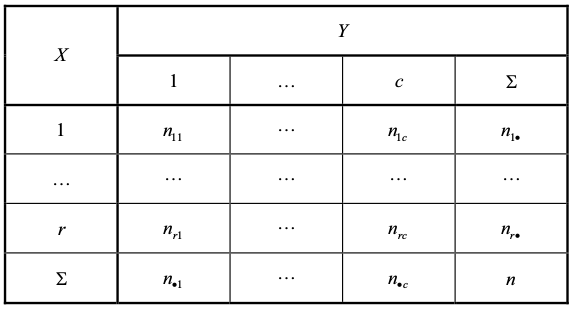
\includegraphics[width=0.8\textwidth]{Obrazky/kontingencni_tabulka.png}
\caption{Kontingenční tabulka}
\end{figure}

\textbf{Test nezávislosti $X$ a $Y$}

Je ekvivalentní testu $H_0: p_{ij} = p_{i \boldsymbol{\cdot}} p_{\boldsymbol{\cdot} j}, \forall (i,j)$, kde $p_{i \boldsymbol{\cdot}} = \sum_j p_{ij}, p_{\boldsymbol{\cdot} j} = \sum_i p_{ij}$ jsou marginální pravděpodobnosti složek $X$ a $Y$ náhodného vektoru $(X,Y)$. Hypotézu $H_0$ testujeme pomocí Pearsonova testového kritéria
\begin{equation*}
\chi^2 = \sum_{i = 1}^r \sum_{ j = 1}^c \frac{(n_{ij} - \frac{n_{i \boldsymbol{\cdot}} n_{\boldsymbol{\cdot} j}}{n})^2}{\frac{n_{i \boldsymbol{\cdot}} n_{\boldsymbol{\cdot} j}}{n}} = n \sum_{i = 1}^r \sum_{ j = 1}^c \frac{n_{ij}^2}{n_{i \boldsymbol{\cdot}} n_{\boldsymbol{\cdot} j}} - n.
\end{equation*}

Hypotézu $H_0$ nezamítáme na hladině významnosti $\alpha$, jestliže $\chi^2 \in \bar{W}_{\alpha} = \langle 0; \chi^2_{1 - \alpha} ((r - 1)(c - 1)) \rangle$. Tento test je asymptotický, obvykle požadujeme, aby pro dvojici $(i,j)$ bylo $\frac{n_{i \boldsymbol{\cdot}} n_{\boldsymbol{\cdot} j}}{n} > 5$.

%\itemize{\textbf{Zdroje:}}
%    \item Anděl, J., Základy matematické statistiky, Praha 2013
%    \item Hübnerová, Z., Studijní materiály pro SP3, Brno 2016

\textbf{Test homogenity}

Testujeme hypotézu, ze pozorované četnosti ve všech řádcích kontingenční tabulky mají multinomické rozdělení s parametry $n_{i \boldsymbol{\cdot}}$ a stejnými pravděpodobnostmi $q_j = p_{1j} = \ldots = p_{rj}$ pro $j = 1, \ldots, c$.

Jestliže $r = c = 2$, jde o tzv. čtyřpolní tabulku pro alternativní (dichotomické) statistické znaky $X$ a $Y$, např. odpovědi respondentů, "ano" nebo "ne".

%%%%%%%%%%%%%%%%%%%%%%%%%%%%%%%%%%%%%
\section{Digitální obraz}

\section{Stochastické procesy}

\section{Filtrace obrazu}

\section{Segmentace a rozpoznávání objektu}



\section{Statistika pro loosery 5.2}
\begin{notes}
Alternativní definice podle Zuzany
\end{notes}
\begin{definition}{(\textbf{Náhodná veličina})}
Nechť $( \Omega, \mathcal{A}) $ je jevové pole a $(\mathbb{R}, \mathcal{B})$ je měřitelný prostor ( tj. $\mathcal{B}$ je borelovská $\sigma$-algebra). Zobrazení $X:\Omega \rightarrow \mathbb{R}$ se nazývá \textit{náhodná veličina} vzhledem k $\mathcal{A}$ právě, když úplný vzor každé borelovské množiny je jev vzhledem k $\mathcal{A}$, tj.
\begin{equation*}
\forall B \in \mathcal{B}: X^{inv }(B):=\{\omega\in \Omega : X(\omega)\in B \}\in \mathcal{A}
\end{equation*}
\end{definition}

\begin{theorem}
Nechť $( \Omega, \mathcal{A}) $ je jevové pole a $(\mathbb{R}, \mathcal{B})$ je měřitelný prostor ( tj. $\mathcal{B}$ je borelovská $\sigma$-algebra). Zobrazení $X:\Omega \rightarrow \mathbb{R}$ se nazývá \textit{náhodná veličina} vzhledem k $\mathcal{A}$ právě, když 
\begin{equation}
\forall x \in \mathbb{R} : \{ \omega \in \Omega: X(\omega)< x\}\in \mathcal{A}
\end{equation}
\end{theorem}


\begin{table}[h]
\centering
\caption{My caption}
\label{my-label}
\begin{tabular}{lll}
jev &zkrácený zápis jevu  & pravděpodobnost  \\
\hline
$\omega:X(\omega)\in B$ &$X\in B$  &$\textbf{P}(X\in B)$  \\
$\omega:X(\omega)< x$ &$X < x$  &$\textbf{P}(X<x)$  \\
$\omega:X(\omega)=x $ &$X=x$  &$\textbf{P}(X=x)$  
\end{tabular}
\end{table}



\begin{definition}
Nechť $(\Omega,\mathcal{A},\textbf{P})$ je pravděpodobnostní prostor a nechť $X$ je náhodná veličina vzhledem k $\mathcal{A}$. Pravděpodobnost $\textbf{P}_x:\mathcal{B}\rightarrow \mathbb{R}, \textbf{P}_x(B)=\textbf{P}(X\in B), \forall B\in \mathcal{B}$ se nazývá rozdělení pravděpodobnosti náhodné veličiny $X$
\end{definition}



\begin{definition}
Nechť $(\Omega,\mathcal{A},\textbf{P})$ je pravděpodobnostní prostor a nechť $X$ je náhodná veličina vzhledem k $\mathcal{A}$. Pak funkci $F_X(x)=\textbf{P}(X<x)$ definovanou pro každé $x\in \mathbb{R}  $ nazýváme distribuční funkcí náhodné veličiny $X$.
\end{definition}

\begin{theorem}
Nechť $(\Omega,\mathcal{A},\textbf{P})$ je pravděpodobnostní prostor a nechť $F(x)$ je její distribuční funkce. pak platí
\begin{enumerate}
\item $0\leq F(x)\leq 1\forall x \in \mathbb{R}$
\item F(x) je neklesající funkce
\item F(x) je zleva spojitá
\item $\lim_{x\rightarrow \infty}F(x)=1$ a  $\lim_{x\rightarrow -\infty}F(x)=0$
\item Pro libovolné $x_1,x_2 \in \mathbb{R}, x_1<x_2$ platí $\textbf{P}(x_1\leq X<x_2)=F(x_2)-F(x_1)$
\item $\forall a \in \mathbb{R}$ platí $\textbf{P}(X=a)=\lim_{x\rightarrow a^+} F(x)-F(x)$
\item $F(x)$ má nejvýše spočetně mnoho bodů nespojitosti
\item $\textbf{P}(a\leq X)=1-F(a) \forall a \in \mathbb{R}$
\item $P(X\leq a) = \lim_{x\rightarrow a^+} F(x) , \forall a \in \mathbb{R}$
\end{enumerate}
\end{theorem}

\begin{notes}
Z $(6)$ plyne, že distribuční funkce je v bodě $x$ spojitá $\Leftrightarrow \textbf{P}(X=x)=0$ 
\end{notes}


\begin{notes}
Mezi $\textbf{P}_X$ a $F$ je vzájemně jednoznačný vztah. řekneme, že distribuční funkce určuje rozdělení pravděpodobnosti náhodné veličiny $X$. Lebesgue-Stieltjes integrál: $\textbf{P}_X(B)=\int_B \mathrm{d}F(x)$
\end{notes}

\begin{theorem}
Má-li funkce $F(x):\mathbb{R}\rightarrow \mathbb{R} vlastnosti (2),(3) $ a $(4)$, pak existuje pravděpodobnostní prostor $\Omega,\mathcal{A},\textbf{P})$ a na něm definovaná náhodná veličina $X$ tak, že $F(x)$ je její distribuční funkcí.
\end{theorem}



\subsection{Diskrétní a spojité náhodné veličiny}
\begin{definition}
Nechť $(\Omega,\mathcal{A},\textbf{P})$ je pravděpodobnostní prostor.  Řekneme, že náhodná veličina $X$ je diskrétní (vzhledem k $P$) právě tehdy, když existuje neprázdná nejvýše spočetná množina $M \subset \mathbb{R}$ taková, že $\textbf{P}_X(M)=1$. Množina $M$ se nazývá obor hodnot a funkce \begin{equation}
p(x)=\textbf{P}(X=x),x\in \mathbb{R}
\end{equation}
se nazývá pravděpodobnostní funkcí diskrétní náhodné veličiny $X$.
\end{definition}

\begin{theorem}
Nechť $X$ je diskrétní náhodná veličina, která má obor hodnot $M$, pravděpodobnostní funkci $p$ a distribuční funkci $F(x)$. pak
\begin{enumerate}
\item $\forall x \in \mathbb{R}: p(x)\geq 0$ (nezápornost)
\item $\sum_{x\in M} p(x) =1$ (normovanost)
\item $F(x)=\sum_{y\in M \cap (-\infty,x\rangle } p(y) $ pro každé $x \in \mathbb{R}$
\item $P(X\in B)=\sum_{y\in M \cap B } p(y) $ pro každé $B \in \mathcal{B}$
\item $p(x) \leq 1$
\item $p(x)= \lim_{t\rightarrow x^+ }F(t)-F(x)$

\end{enumerate}
\end{theorem}

\begin{notes}
Distribuční funkce diskrétní náhodné veličiny má schodovitý průběh a určuje pravděpodobnostní funkci jednoznačně (viz $(6)$).
\end{notes}

\begin{theorem}
Nechť reálná funkce $p(x)$ má vlastnosti $(1),(2)$, pak existuje pravděpodobnostní prostor a na něm definovaná diskrétní náhodná veličina $X$ taková, že $p(x)$ je její pravděpodobnostní funkce.
\end{theorem}


\begin{definition}
Nechť $(\Omega,\mathcal{A},\textbf{P})$ je pravděpodobnostní prostor. Řekneme, že náhodná veličina $X$ s distribuční funkcí $F(x)$ je \textit{je spojitá} (vzhledem k $\textbf{P}$) právě tehdy, když existuje nezáporná po částech spojitá funkce $f(x)$, že pro $\forall x \in \mathbb{R}$ platí 
\begin{equation}
F(x)=\int_{-\infty}^x f(t)\, \mathrm{d} t.
\end{equation}
Funkce $f(x)$ se nazývá hustota náhodné veličiny $X$.
\end{definition}

\begin{notes}
Distribuční funkce spojité náhodné veličiny $X$ je všude spojitá, protože je funkcí horní meze integrálu.
\end{notes}

\begin{theorem}
Nechť $f(x)$ je hustota spojité náhodné veličiny $X$. Pak 
\begin{enumerate}
\item $f(x)\geq 0, \forall x \in \mathbb{R}$
\item $\int_{-\infty}^{\infty} f(x)\, \mathrm{d} x=1$
\item Pro libovolné ale pevně zvolené $x_0\in \mathbb{R}$ a $h>0 $ platí $P(x_0<X<x_0+h)=\int_{x_0}^{x_0+h}f(x)\, \mathrm{d}x$
\item Pro libovolné ale pevně dané $x_0\in \mathbb{R}$ platí $P(X=x_0)=0$
\item Ve všech bodech spojitosti funkce $f(x)$ platí$ \mathrm{d}F(x)/\mathrm{d}x$
\end{enumerate}
\end{theorem}

\begin{theorem}
Jestliže reálná funkce $f(x)$ má vlastnosti $(1),(2)$, pak existuje pravděpodobnostní prostor $(\Omega,\mathcal{A},\textbf{P})$ a na něm definovaná spojitá náhodná veličina $X$ tak, že $f(x)$ je její hustota.
\end{theorem}

\subsection{Rozdělení transformovaných náhodných veličin}
\begin{theorem}
Nechť $(\Omega, \mathcal{A})$ je jevová $\sigma$-algebra a $(\mathbb{R},\mathcal{B})$ je měřitelný prostor, $X:\Omega\rightarrow \mathbb{R}$ je náhodná veličina a $g:\mathbb{R}\rightarrow\mathbb{R}$ je borelovská funkce (tj. úplný vzor $\forall B \in \mathcal{B}$ je z $\mathbb{B}$). Pak složené zobrazení $Y:\Omega\rightarrow \mathbb{R}$ dané vzorcem $\forall \omega \in \Omega: Y(\omega)=g(X(\omega))$ je náhodná veličina (vzhledem k $\mathcal{A}$). zobrazení $Y$ nazýváme transformovaná náhodná veličina.
 \end{theorem}
 
 \begin{theorem}
 Nechť náhodná veličina $X$ má distribuční funkci $F_X$ a nechť $g$ je borelovská funkce. Pak transformovaná náhodná veličina $Y=g(X)$ má distribuční funkci $F_Y(y)=\int_{B_y}\mathrm{d}F(x)$, kde $B_y=\{x:h(x)<y) \}$
 \end{theorem}

\begin{notes}
Pro diskrétní veličinu $X$ s pravděpodobnostní funkcí $p$ lze $F_Y$ stanovit jako $F_Y(y)=\sum_{x\in M\cap B_y}p(x)$
\end{notes}

\begin{notes}
Pro spojitou náhodnou veličinu $X$ s hustotou $f$ lze $F_y$ stanovit jako $F_Y(y)=\int_{xB_y} f(x)\mathrm{d}x.$
\end{notes}

\begin{theorem}
Nechť náhodná veličina $X$ je diskrétní, má pravděpodobnostní  funkci $p_X$ a nechť $g$ je borelovská funkce. Pak transformovaná náhodná veličina $Y=g(X)$ má pravděpodobnostní funkci $p_Y(y)=\sum_{x\in M \cap C_y}p_X(x)$, kde $C_y=\{x:h(x)=y\}$
\end{theorem}

\begin{theorem}
Nechť náhodná veličina $X$ je spojitá a má hustotu $f_X$. Dále nechť $g$ je vzájemně jednoznačná borelovská funkce a existuje spojitá derivace její inverze $\mathrm{d}g^{-1}(y)/\mathrm{d}y$. Pak transformovaná náhodná veličina $Y=g(X)$ má hustotu $f_Y(y)=f_X(g^{-1}(y))|\mathrm{d}g^{-1}(y)/\mathrm{d}y|$. 
\end{theorem}

\subsection{Číselné charakteristiky}
\begin{definition}
Nechť $X$ je náhodná veličina na $(\Omega,\mathcal{A},\textbf{P})$ s distribuční funkcí $F_X$. Pak střední hodnotou náhodné veličiny $X$ je
\begin{equation}
\mathrm{E}(x)=\int_{-\infty}^{\infty} x\mathrm{d}F(x)
\end{equation}
pokud tento integrál existuje a je konečný. Není-li integrál konečný nebo neexistuje, říkáme, že střední hodnota $EX$ neexistuje. ($EX$ charakterizuje polohu náhodné veličiny $X$ na číselné ose, těžiště)
\end{definition}

\begin{enumerate}
\item Je-li $X$ diskrétní s pravděpodobnostní funkcí $p(x)$, pak $\mathrm{E}(X)=\sum_{x\in M}xp(x).$
\item Je-li $X$ spojitá s hustotou $f(x)$, pak $\mathrm{E}(X)=\int_{-\infty}^{\infty} x f(x)\mathrm{d}x .$
\end{enumerate}

\begin{theorem}[Výpočet střední hodnoty transformované náhodné veličiny]
Nechť $X$ je náhodná veličina, $g:\mathbb{R}\rightarrow \mathbb{R}$ borelovská, $Y=g(X)$ je transformovaná náhodná veličina. Pak
\begin{equation}
\mathrm{E}Y=\int_{-\infty}^{\infty}g(x)\mathrm{d}F_X(x),
\end{equation}
pokud integrál existuje.
\begin{enumerate}
\item Je-li $X$ diskrétní s pravděpodobnostní funkcí$p(x)$, pak $\mathrm{E}(Y)=\sum_{x\in M} g(x)p(x)$
\item Je-li $X$ spojitá s hustotou $f(x)$, pak $\mathrm{E}(Y)=\int_{-\infty}^{\infty} g(x)f(x)\mathrm{d}x.$
\end{enumerate}
\end{theorem}

\begin{theorem}
Nechť $a,b \in \mathbb{R},X$ je náhodná veličina. Pak
\begin{enumerate}
\item $\mathrm{E}(a)=a$
\item Existuje-li $\mathrm{E}(X)$, pak $\mathrm{E}(a+bX)=a+b\mathrm{E}(X)$
\item Existuje-li $\mathrm{E}(X)$, pak $\mathrm{E}(X-\mathrm{E}X)=0$
\item Nechť $\textbf{P}(X=a)=1$, pak $\mathrm{E}X=a$
\item Nechť $\textbf{P}(X\geq 0)=1$, pak $\mathrm{E}X\geq 0.$
\end{enumerate}
\end{theorem}

\begin{definition}
Nechť $X$ je náhodná veličina na $(\Omega,\mathcal{A},\textbf{P})$. Rozptylem náhodné veličiny $X$ rozumíme číslo 
\begin{equation}
\mathrm{D}(X)=\mathrm{E}[X-\mathrm{E} X]^2
\end{equation}
za předpokladu, že střední hodnota vpravo existuje. Číslo $\sqrt{\mathrm{D}(X)}$ se nazývá směrodatná odchylka. Náhodná veličina $X-\mathrm{E} X$ se nazývá centrovaná náhodná veličina. Náhodná veličina $\frac{X-\mathrm{E}X}{\sqrt{\mathrm{D}X}}$ se nazývá standardizovaná náhodná veličina. (Rozptyl charakterizuje variabilitu číselných realizací náhodné veličiny $X$ kolem její střední hodnoty $\mathrm{E}X$ s přihlédnutím k pravděpodobnostem)
\end{definition}

\begin{dusledek}
$\mathrm{D}(X)=\int_{-\infty}^{\infty}(x-\mathrm{E}X)^2\mathrm{d}F(x)$
\begin{enumerate}
\item Je-li $X$ diskrétní náhodná veličina s pravděpodobnostní funkcí $p(x)$, pak $\mathrm{D}(X)=\sum_{x\in M}(x-\mathrm{E}X)^2p(x)$ za předpokladu, že $\mathrm{E}X$ existuje a suma absolutně konverguje.
\item 
Je-li $X$ spojitá náhodná veličina s hustotou $f(x)$, pak $\mathrm{D}(X)=\int_{-\infty}^{\infty}(x-\mathrm{E}X)^2f(x)\mathrm{d}x$ za předpokladu, že $\mathrm{E}X$ existuje a integrál absolutně konverguje.
\end{enumerate}
\end{dusledek}

\begin{theorem}
Nechť $a,b \in \mathbb{R}, X$ je náhodná veličina. Pak
\begin{enumerate}
\item $\mathrm{D}(a)=0$
\item Existuje-li $\mathrm{E}(X)^2< \infty$, pak $\mathrm{D}(a+bX)=b^2\mathrm{D}(X)$
\item $\mathrm{D}(X)=\mathrm{E}(X^2)-(\mathrm{E}X)^2$
\item $\mathrm{D}(X)\geq 0$ a rovnosti je dosaženo právě tehdy, když $\textbf{P}(X=\mathrm{E}X)=1$
\item $\mathrm{E}(X-a)^2 \geq \mathrm{D}X$ a rovnosti je dosaženo právě tehdy, když $\mathrm{E}X=a$ 
\end{enumerate}
\end{theorem}

\begin{definition}
Nechť $X$ je náhodná veličina na $(\Omega,\mathcal{A},\textbf{P})$. Číslo $\mathrm{E}[(X-k)^r]$ se nazývá $r$-tý moment náhodné veličiny $X$.
\end{definition}
\begin{enumerate}
\item Je-li $k=0$ mluvíme o obecném momentu (označíme $\mu_k'$). Je-li $k=\mathrm{E}X$ mluvíme o centrálním momentu (označíme $\mu_k$)
\item Číslo $A_3=\frac{\mathrm{E}(X-\mathrm{E}X)^3}{\sqrt{\mathrm{D}X}^3}$ se nazývá šikmost. (Charakteristika symetrie náhodné veličiny $X$ okolo $\mathrm{E}X$. Při $A_3=0$ mluvíme o symetrickém rozdělení
\item Číslo $A_4=\frac{\mathrm{E}(X-\mathrm{E}X)^4}{\sqrt{\mathrm{D}X}^4}-3$ se nazývá špičatost. (Charakteristika špičatosti náhodné veličiny $X$ ve srovnání se standardním normálním rozdělením). Náhodná veličina se standardním normálním rozdělením má $A_4=0$.
\end{enumerate}

\begin{theorem}[Markovova nerovnost] Nechť $\textbf{P}(X \geq 0) = 1$   a $\mathrm{E}(X)$ existuje. Pak pro $\forall \varepsilon > 0: \textbf{P}(X>\varepsilon\mathrm{E}X) \leq \frac{1}{\varepsilon}$
Využívá se k odhadu $\mathbb{P}(X>\varepsilon\mathrm{E}X)$, když neznáme $\textbf{P}_X$, ale jen $\mathrm{E}X$
\end{theorem}

\begin{theorem}[Čebyševova nerovnost] Nechť $X$ je náhodná veličina, $\mathrm{E}X$ a $\mathrm{D}X$ existují. Pak pro $\forall t > 0 : \textbf{P}(|X-\mathrm{E}X|>t\sqrt{\mathrm{D}X})\geq \frac{1}{t^2}$.
Využívá se k odhadu $\textbf{P}(|X-\mathrm{E}X|>c$, když neznáme $P_X$, ale jen $\mathrm{E}X, \mathrm{D}X$ 
\end{theorem}


\begin{notes}
$\mathrm{E}X$, medián a modus jsou tzv. \textit{číselné charakteristiky polohy} a $\mathrm{D}X$, šikmost a špičatost jsou tzv. \textit{číselné charakteristiky variability}
\end{notes}


\begin{theorem}
Nechť $F(x)$ je distribuční funkce náhodné veličiny $X: \Omega \rightarrow \mathbb{R}$ na  $(\Omega,\mathcal{A},\textbf{P})$. Pak funkci $F^{-1}(u)= \min \{x:F(x)\geq u\}, 0 <u<1$ nazýváme kvantilovou funkci a její hodnoty kvantily:
\begin{table}[h]
\centering
\caption{Kvantily}
\begin{tabular}{ll}
$x_{0.5}=F^{-1}(0.5)$ & medián  \\
$x_{0.25}=F^{-1}(0.25),F^{-1}(0.75)$ & dolní, horní kvantil  \\
$F^{-1}(0.1),F^{-1}(0.9)$ & decily  \\
$F^{-1}(0.01),F^{-1}(0.99)$ & percentily  \\
$F^{-1}(0.75)-F^{-1}(0.25)$ & kvantilová odchylka
\end{tabular}
\end{table}
\end{theorem}


\begin{notes}
Nechť $X$ je spojitá náhodná veličina s distribuční funkcí $F(x)$ a hustotou $f(x)$, pak pro kvantilovou funkci platí\begin{equation}
F(F^{-1}(\alpha))=\alpha=\int_{-\infty}^{F^{-1}(\alpha)}f(x)\mathrm{d}x
\end{equation}
\end{notes}

\subsection{Vybraná rozdělení diskrétní náhodné veličiny}
\begin{definition}{\textbf{(Binomické rozdělení}}
Buď $n$ přirozené číslo a $p \in (0, 1)$. Předpokládejme, že $X$ nabývá pouze hodnot $0, 1, ..., n$ a to s pravděpodobnostmi
\begin{equation}
\textbf{P}(X = k) = \binom{n}{k}p^{k}(1-p)^{n-k}, \enskip k = 0, 1, ..., n.
\end{equation}
Pak říkáme, že $X$ má binomické rozdělení a píšeme $X \sim Bi(n,p)$.
\end{definition}
\begin{proposition}
Nechť  $X \sim Bi(n,p)$. potom $\mathbf{E}X = np$, $\mathbf{var}X = np(1-p)$ a $\psi(t) = (1-p + pe^{it})^{n}$.
\end{proposition}
\begin{proof}
Důkaz se mi nechce dělat, ukáže se to tak, že se nějakými manipulacemi s nekonečnou řadou vyjadřující střední hodnotu získá její součet, rozptyl podobně. Char fce. z definice
\end{proof}

\begin{remark}
Binomické rozdělení je diskrétní rozdělení pravděpodobnosti počtu úspěšných pokusů v posloupnosti $n$ nezávislých pokusů.
Modeluje počet úspěchů ve výběru velikosti $n$ z populace o velikosti $N$ s vracením. Př.: Mám osudí s bílými a černými míčky $n$-krát vytáhnu z osudí míček, poznamenám si barvu a vrátím ho zpět, bin. rozd. udává pravděpodobnost že $k$ míčků bude černých (resp. bílých). Pro $n = 1$ se jedná o tzv alternativní rozdělení.
\end{remark}
\begin{definition}[Alternativní rozdělení]
$X \sim A(p)$ odpovídá $X\sim \mathrm{Bi}(1,p)$. Náhodná veličina $X$ udává počet úspěchů při jednom pokusu, přičemž pravděpodobnost úspěchu je $p, p\in (0,1)$
\end{definition}

\begin{definition}{\textbf{(Hypergeometrické rozdělení)}}
Nechť $N, A$ a $n$ jsou přirozená čísla, přičemž $A < N, n < N$. Nechť $X$ nabývá pouze celočíselných hodnot s pravděpodobnostmi 
\begin{equation}
\textbf{P}(X = x)= \frac{\binom{A}{k}\binom{N-A}{n-k}}{\binom{N}{n}} \enskip pro \enskip \max(0, A + n -N)\leq k \leq \min(A, n).
\end{equation}
Pak říkáme, že $X$ má hypergeometrické rozdělení a píšeme $X \sim Hg(N,A,n)$.
\end{definition}
\begin{proposition}
Nechť $X$ má hypergeometrické rozdělení s parametry $N, A$ a $n$, přičemž $A < N, n < N$.  Je-li $N > 1,$ pak 
\begin{equation}
\mathbf{E}X = \frac{nA}{N}, \enskip \mathbf{var}X = \frac{nA(N-A)}{N^{2}}\bigg( 1 - \frac{n-1}{N-1}\bigg).
\end{equation}
\end{proposition}
\begin{proof}
Důkaz je ponechán pro zvídavého čtenáře, jenž je laskavě odkázán, na literaturu zabývající se pravděpodobností a statistikou.
\end{proof}

\begin{remark}
Poznamenejme, že hypergeometrické rozdělení modeluje pravděpodobnost počtu úspěchů ve výběru velikosti $n$ z populace o velikosti $N$ za předpokladu, že výběr probíhá bez opakování. V případě osudí s míčky z příkladu u binomického rozdělení bychom míčky po vytažení již nevraceli zpět.
\end{remark}

\begin{definition}{\textbf{(Poissonovo rozdělení)}}
Nechť $X$ nabývá pouze hodnot $0, 1, ..., $ a to s pravděpodobnostmi 
\begin{equation}
\textbf{P}(X = k) = \frac{\lambda^{k}}{k!}e^{-\lambda},\enskip k = 0, 1, ...,
\end{equation}
kde $\lambda >0$ je dané číslo. Pak říkáme, že $X$ má Poissonovo rozdělení s parametrem $\lambda$ a píšeme $X \sim Po(\lambda)$.
\end{definition}

\begin{proposition}
Nechť $X \sim Po(\lambda)$. Potom $\mathbf{E}X = \lambda,$ $\mathbf{var}X = \lambda$ a $\psi(t) = e^{\lambda(e^{it}-1)}$.
\end{proposition}
\begin{proof}
Důkaz prvních dvou je z definice manipulací s nekonečnými řadami pro získání jejich součtu, třetí z definice char. fce. Toto mám dokonce naTeXované, ale dávat to sem nebudu, anžto je to delší. Kdyby to někoho hrozně strašně moc zajímalo, nechť se zeptá.
\end{proof}
\begin{remark}
Popisuje pravděpodobnost nastání daného počtu nezávislých jevů v určitém časovém intervalu. Například pravděpodobnost obdržení určitého počtu spamových emailů za týden, za předpokladu, že každý email je na všech ostatních nezávislý.
\end{remark}



\begin{definition}{\textbf{(Geometrické rozdělení)}}
$X\sim \mathrm{Ge}(p)$. Náhodná veličina $X$ počet neúspěchů předcházejících prvnímu úspěchu v posloupnosti opakovaných nezávislých pokusů, přičemž pravděpodobnost úspěchu je v každém pokusu $p, p\in (0,1)$
\begin{equation}
p(x)=(1-p)^xp \text{,    pro x=0,1,2,\ldots}
\end{equation}
 a $0$ jinak.
\end{definition}

\begin{proposition}
Nechť $X \sim \mathrm{Ge}(p)$. Potom $\mathbf{E}X =(1-p)/p,$ $\mathbf{D}X = (1-p)/p^2$ 
\end{proposition}




\subsection{Spojitá rozdělení pravděpodobnosti}
\begin{definition}{\textbf{(Normální rozdělení)}}
Nechť $ \mu \in \mathbb{R}$ a $\sigma > 0$ jsou dané konstanty (parametry). Normální rozdělení je určeno hustotou
\begin{equation}
f(x) = \frac{1}{\sqrt{2\pi}\sigma}\exp \bigg[ -\frac{(x - \mu)^{2}}{2\sigma^{2}} \bigg]
\end{equation}
a označuje se symbolem $N(\mu, \sigma^{2}).$ V případě, že $\mu = 0$ a $\sigma = 1$ nazýváme $N(0, 1)$ standardní normální rozdělení, jeho hustotu značíme $\phi$ a příslušnou distribuční funkci $\Phi$, máme tedy
\begin{equation}
\phi(x) = \frac{1}{\sqrt{2\pi}}e^{\frac{-x^{2}}{2}}, \enskip \Phi(x) = \int_{-\infty}^{x}\phi(t)dt.
\end{equation}
\end{definition}

\begin{proposition}
Nechť $X \sim N(\mu, \sigma^{2})$ potom $\mathbf{E}X = \mu$, $\mathbf{var}X = \sigma^{2}$, šikmost $\alpha_{3} = 0$ a špičatost $\alpha_{4} = 3$. Charakteristická funkce normálního rozdělení má tvar 
\begin{equation}
\psi(t) = \exp\bigg[ i\mu t - \frac{1}{2}\sigma^{2}t^{2} \bigg].
\end{equation}
\end{proposition}
\begin{proof}
Přímým výpočtem.
\end{proof}

\begin{remark}
Normální rozdělení má v matematické statistice a stochastické analýze veliký význam, mnoho statistických modelů je založeno na předpokladu normálního rozdělení. Příkladem je třeba regrese, kde se předpokládá normální rozdělení závisle proměnných, aby bylo možné odvodit intervaly spolehlivosti, nebo testy vycházející z regresní analýzy, např. analýza rozptylu. V této souvislosti připomeňme také centrální limitní větu, která říká, že průměry z výběrů z nezávislých rozdělení konvergují v distribuci k normálnímu rozdělení.
\end{remark}

\begin{definition}{\textbf{(Weibullovo rozdělení)}}
Nechť $c > 0, \enskip p > 0$. Weibullovi rozdělení $W(c, p)$ má hustotu
\begin{equation}
f(x) = cpx^{p-1}\exp[-cx^{p}], \enskip x > 0.
\end{equation}
Pro volbu $p = 1$ získáme exponenciální rozdělení.
\end{definition}

\begin{proposition}
Nechť $X \sim W(c, p)$, platí
\begin{equation}
\mathbf{E}X = \Gamma\bigg( \frac{p + 1}{p} \bigg) c^{-1/p}, \enskip \mathbf{var}X = \bigg[ \Gamma \bigg( \frac{p+2}{p}\bigg) - \Gamma^{2} \bigg( \frac{p + 1}{p}\bigg) \bigg] c^{-2/p}, 
\end{equation}
kde $\Gamma$ je gamma funkce definovaná pro $a>0$ předpisem $\Gamma(a) = \int_{0}^{\infty} x^{a - 1}e^{-x}dx.$
\end{proposition}

\begin{remark}
Weibullovo rozdělení se využívá ve spolehlivosti při modelování životnosti. Dobře vystihuje dobu do poruchy stárnoucího objektu.
\end{remark}







\subsection{Charakteristická funkce}
\begin{definition}
Nechť $X,Y$ jsou náhodné veličiny definované na $(\Omega,\mathcal{A},\textbf{P})$.\begin{equation}
Z=X+iY, Z:\Omega\rightarrow\mathbb{C}
\end{equation}
Pak $Z=X+iY$ nazýváme komplexní náhodná veličina- Navíc, pokud existují $\mathrm{E}X$ a $\mathrm{E}Y$, zavedeme $\mathrm{E}Z=\mathrm{E}X+i\mathrm{E}Y$ střední hodnotu komplexní náhodné veličiny.
\end{definition}


\begin{definition}
Funkci \begin{equation}
\psi =\mathrm{E}(\mathrm{e}^{itX}=\mathrm{E}(\cos(tX)+i\sin(tX))=\mathrm{E}(\cos(tX))+i\mathrm{E}(\sin(tX)), t\in \mathbb{R},
\end{equation}
nazveme charakteristickou funkcí náhodné veličiny $X,\psi:\mathbb{R}\rightarrow\mathbb{C}$
\end{definition}

\begin{notes}
Má-li $X$ distribuční funkci $F(x)$
\begin{equation}
\psi(t)=\int_{-\infty}^{\infty}\mathrm{e}^{itX} \mathrm{d}F(x)
\end{equation}
Pro diskrétní veličinu $X$ s pravděpodobnostní funkcí $p(x)$:
\begin{equation}
\psi(t)=\sum_M \mathrm{e}^{itX}p(x)=\sum_M\cos(tX)p(x)+i\sum_M\sin(tX)p(x)
\end{equation}
Pro spojitou veličinu $X$ s hustotou $f(x)$\begin{equation}
\psi(t)=\int_{-\infty}^{\infty}\mathrm{e}^{itX}f(x) \mathrm{d}x =\int_{-\infty}^{\infty}\cos(tX) f(x) \mathrm{d}x+i\int_{-\infty}^{\infty}\sin(tX) f(x) \mathrm{d}x
\end{equation}
\end{notes}


\begin{theorem}
Vlastnosti charakteristické funkce
\begin{enumerate}
\item charakteristická funkce náhodné veličiny je VŽDY definována
\item $\psi(0)=\mathrm{E}(1)=1$
\item $|\psi(t)| \leq 1$
\item $\psi(-t)=\overline{\psi(t)}$
\item $\psi(t)$ je stejnoměrně spojitá na $\mathbb{R}$
\item $a,b \in \mathbb{R}$, pak $Y=a+bX$ má charakteristickou funkci $\psi_Y(t)=\mathrm{e}^{iat}\psi(bt)$
\end{enumerate}
\end{theorem}

\begin{theorem}
Jestliže $X_1,X_2$ jsou nezávislé, pak charakteristická funkce $S=X_1+X_2$ je rovna $\psi_S(t)=\psi_{X_1}(t)\psi_{X_2}(t)$, kde $\psi_{X_j}(t)$ značí charakteristickou funkci náhodné veličiny $X_j, j=1,2.$
\end{theorem}

\begin{theorem}
Existuje-li $k$-tý obecný moment $\mu_k$, pak existuje $\psi^{(k)}(t)$ ($k$-tá derivace) a platí \begin{equation}
\psi^{(k)}(0)=i^k\mu_k
\end{equation}
\end{theorem}

\begin{dusledek}
Existují-li $k$-tý moment obecný moment $\mu_k$ až do řádu $n$, pak
\begin{equation}
\psi(t)=\sum_{k=0}^{n}\frac{(it)^k}{k!} \mu_k+o(t^n),
\end{equation}
kde $\mu_0=1$ a o je funkce malé o, tj. $o(t):\lim_{t\rightarrow 0}\frac{o(t)}{t}=0$
\end{dusledek}


\end{document}